\documentclass[11pt,a4paper,twoside]{book}
\usepackage{setspace}
\usepackage{ccicons}
\usepackage{amsmath}
\usepackage{apacite}
\usepackage{dirtytalk}
\usepackage{titlepic}
\usepackage{graphicx}
\usepackage[sort&compress,round]{natbib}
\usepackage[labelfont=bf, labelsep=period, skip=2pt]{caption}
\usepackage[margin=3cm]{geometry}
\usepackage[english]{babel}
\usepackage{amssymb}
\usepackage{textcomp}
\usepackage{siunitx}
\usepackage{relsize}
\newcommand{\norm}[1]{\left\lVert#1\right\rVert}
\usepackage[toc,page]{appendix}
%\setcounter{secnumdepth}{0}
\usepackage{array}

% use Unicode characters - try changing the option if you run into troubles with special characters (e.g., umlauts)
\usepackage{mathtools}
\usepackage{isomath}
\usepackage{amssymb}
\usepackage{amsmath}
\usepackage{todonotes}
\usepackage{graphicx}
\usepackage{gensymb}

% hyperref makes references clicky. use \url{www.example.com} or \href{www.example.com}{description} to add a clicky url
\usepackage{nameref,hyperref}
\usepackage{url}  % This makes \url work
\PassOptionsToPackage{hyphens}{url}\usepackage{hyperref}
%\usepackage{nohyperref}  % This makes hyperref commands do nothing without errors
\usepackage[utf8]{inputenc}
\hypersetup{draft}


%\usepackage[superscript, compress]{cite}


%embed youtube videos
\usepackage{media9}

% improves typesetting in LaTeX
\usepackage{microtype}
\DisableLigatures[f]{encoding = *, family = * }


% adjust caption style
\usepackage[aboveskip=1pt,labelfont=bf,labelsep=period,singlelinecheck=off]{caption}
% this is required to include graphics
\usepackage{graphicx}

\usepackage{amsmath}
\DeclareMathOperator*{\argmax}{arg\,max}
\DeclareMathOperator*{\argmin}{arg\,min}

\newcommand\blfootnote[1]{%
  \begingroup
  \renewcommand\thefootnote{}\footnote{#1}%
  \addtocounter{footnote}{-1}%
  \endgroup
}

\title{
	\HUGE \textbf{Computer Vision and Deep Learning Methods for Measuring and Modeling Animal Behavior} \\
	\vspace{4cm}
	\Large Dissertation submitted \\
	\Large for the academic degree of \\
	\vspace{0.5cm}
	\Large \textit{Doctor of Natural Sciences} \\

	\vspace{2cm}
    \Large Presented by \\
    \vspace{0.5cm}
    \LARGE Jacob M. Graving \\
    \vspace{0.5cm}
    \Large at the \\
    \vspace{0.1cm}
	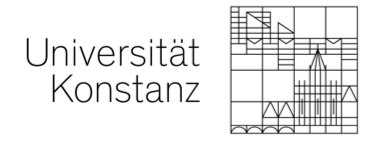
\includegraphics[width=6cm]{Graving_IMPRS_Thesis/graphics/uni_logo.png}\\
	\vspace{2cm}
	\Large Faculty of Science \\
	\Large Department of Biology \\
	\vspace{2cm}
	\Large Konstanz, 2020
	\date{}
}

\begin{document}
	\maketitle
	\pagenumbering{gobble}
    \newpage
    Page intentionally left blank
    \newpage
	\tableofcontents
	\setcounter{page}{1}
	\pagenumbering{roman}
\begin{doublespace}
	\chapter*{Summary}
	\markboth{SUMMARY}{SUMMARY}
	\addcontentsline{toc}{chapter}{Summary}
  The study of animal behavior is a fundamental pursuit for answering scientific questions across a variety of fields --- including neuroscience, psychology, ecology, genetics, and evolution. While the task of collecting accurate and complete behavioral data has typically always been difficult, laborious, and subjective, in recent years there has been rapid progress in methods for automatically quantifying behavior objectively and at scale. This progress has been primarily driven by the emergence of new computational hardware for imaging and sensing body movement in conjunction with new computational software and algorithms for measuring behavior. With the increased quality and resolution of these data comes the need for new methods for data-driven modeling that can reveal core insights into the behavior of animals. The focus of this thesis is on tools— the development of new computational algorithms and software— for measuring and modelling behavior using methods from computer vision, deep learning, Bayesian inference, and probabilistic programming, while also synthesizing these approaches with ideas from areas such as information theory, nonlinear dynamics, and statistical physics. The three chapters describe computer vision and deep learning methods for measuring behavior in the laboratory and field (Chapters 1 and 2) as well as methods for using these data to model behavior with modern techniques from machine learning and Bayesian statistical inference (Chapter 3). Together these methods allow researchers to answer scientific questions that were previously intractable.

	\chapter*{Zussamenfassung}
	\markboth{ZUSSAMENFASSUNG}{ZUSSAMENFASSUNG}
    \addcontentsline{toc}{chapter}{Zussamenfassung}
  Das Studium des Verhaltens von Tieren ist ein grundlegendes Bestreben zur Beantwortung wissenschaftlicher Fragen in einer Vielzahl von Bereichen --- einschließlich Neurowissenschaften, Psychologie, Ökologie, Genetik und Evolution. Während die Aufgabe, genaue und vollständige Verhaltensdaten zu sammeln, in der Regel immer schwierig, mühsam und subjektiv war, gab es in den letzten Jahren rasche Fortschritte bei den Methoden zur automatischen objektiven und maßstabsgetreuen Quantifizierung von Verhalten. Dieser Fortschritt wurde in erster Linie durch das Aufkommen neuer rechnergestützter Hardware, Software und Algorithmen zur Verhaltensmessung vorangetrieben. Mit der zunehmenden Qualität und Auflösung dieser Daten steigt auch der Bedarf an neuen Methoden zur datengesteuerten Modellierung, die zentrale Erkenntnisse darüber liefern können, wie Tiere ihr Verhalten organisieren. In dieser Arbeit konzentriere ich mich auf die Entwicklung neuer Algorithmen und Software zur Messung und Modellierung von Verhalten mit Methoden des Tiefenlernens, der Bayes'schen Inferenz und der probabilistischen Programmierung, wobei ich diese Ansätze auch mit Ideen aus anderen relevanten Bereichen wie Informationstheorie, nichtlineare Dynamik und statistische Physik zusammenführe. Zunächst entwickelte ich in Zusammenarbeit mit Kollegen ein Strichcode-Verfolgungssystem für automatisierte Verhaltensstudien, bei dem der Aufenthaltsort und die Identität von Individuen über längere Zeiträume mit herkömmlicher Computer-Sicht zuverlässig verfolgt werden kann (Kapitel 1). Als nächstes entwickelte ich Mehrzweck-Tiefenlernmethoden für die Messung der Haltung von Tieren --- jede Menge vom Benutzer ausgewählter Körperteile --- im Labor und vor Ort (Kapitel 2). Schließlich stelle ich Methoden zur Verwendung dieser Haltungsdaten zur Verhaltensmodellierung mit Techniken des maschinellen Lernens und der statistischen Bayes'schen Inferenz vor (Kapitel 3). Zusammen verringern diese Methoden die Barrieren bei der Messung und Modellierung des Verhaltens von Tieren und ermöglichen es den Forschern, wissenschaftliche Fragen zu beantworten, die zuvor unlösbar waren.

	\newpage
	\pagenumbering{arabic}
	\chapter*{Introduction}
	\markboth{INTRODUCTION}{INTRODUCTION}
Measuring and modeling behavior are fundamental problems for the study of behavioral ecology and neuroscience. In general, these methodological areas seek to develop techniques capable of answering a straightforward set of questions: where? who? and what? More concretely, where are individuals located in space? Who are those individuals? And what are they doing? Perhaps unsurprisingly, these three fundamental questions overlap with similar unsolved problems in computer vision: namely, object detection and tracking, facial recognition and object classification, as well as pose estimation and action recognition. Despite the concrete, real-world nature of these problems, only very recently have the computational algorithms for solving these tasks reached the same level of quality as that of manual human annotation. This increase in quality is largely due to the democratization and wide-spread adoption of deep learning algorithms, a class of maximum likelihood linear models that are capable of scaling to arbitrarily large and complex datasets. Consequently, a large body of computer science literature with general-purpose algorithms for solving these previously-unsolved tasks now exists, and this progress is only just beginning to be adapted to study animal behavior --- which brings with it many additional unsolved problems.

Just 30 years ago, the use of computer vision for the study of animal behavior was rare. However, as computational hardware and software have matured and became more accessible, so have the methods used to quantify movement and extract insights from behavioral data. Studying behavior with computer vision methods has become increasingly common, and the field of animal behavior has evolved rapidly in response. For example, many of the conventional approaches developed only a few years ago are now almost completely obsolete. The most prevalent approaches now focus on the use of deep learning for the measurement and modelling of animal locomotion --- including automated motion capture and tracking of animal movements in the laboratory and in the wild. This is an extremely exciting and active research area, with researchers continuously advancing a wide range of methods to effectively measure behavior in almost any scenario where a human is capable of solving the task. The overarching goal of this thesis was to contribute to this growing body of work by developing general-purpose, open-source software and algorithms that allow researchers to apply computational tools to measure and model behavior. Over the course of my PhD, I built on the existing deep learning and computer vision literature to develop new software and algorithms for solving these problems. I then collaborated with other researchers to apply these methods to detect, track, and estimate the body posture of animals both in the laboratory and the field. Additionally, I developed methods for summarizing and interpreting these data using probabilistic deep learning models, which draw on fundamental ideas from Bayesian statistics and information theory. Together these methods have allowed researchers to measure behavior in experimental scenarios that were previously intractable and have helped to make meaningful biological inferences using large, complex, high-dimensional data sets.

Deep learning has begun to revolutionize science as we know it. Rapid advances in hardware and software have democratized this class of machine learning algorithms, which, consequently, has made the use of deep learning tools commonplace across the natural sciences. These general-purpose algorithms have been applied to a wide array of problems in computer vision, natural language processing, and audio recognition. With the right data, these methods have the potential to solve nearly any computational task with relatively minimal effort---even those once thought to always require human-level intelligence. The field of animal behavior is no different, and deep learning has dramatically impacted this field in a short period of time. Deep learning has already revolutionized the study of animal behavior as a tool for both quantifying behavior as well as understanding behavior through data-driven modelling and will continue to advance the study of behavior for the foreseeable future. 

In this thesis, I provide an update on the status of computer vision-based methods in the behavioral sciences. I focus on a few of the most prominent methods in this area of research, highlight some of the most promising applications for these technologies, and introduce several advances in the use of computer vision and deep learning-based methods to automatically measure animal locomotion and body posture. First, I discuss methods for tracking the behavior of animals using marker-based spatial localization and individual identification with conventional computer vision techniques, which allowed for the development of an automated barcode tracking system for long-term behavioral studies in captive bird populations. Second, I discuss image-based approaches using deep learning to measure detailed information about animal body posture and introduce a deep learning-based software toolkit, called DeepPoseKit, with general-purpose methods for the automated measurement of animal body posture. Third, I discuss methods for decomposing these detailed behavioral data into underlying constituent components by identifying stereotyped behavioral motifs directly from data. To accomplish this, I introduce a new deep learning model, called VAE-SNE, for general-purpose analysis of high-dimensional data and demonstrate its utility across multiple domains. In particular, I use VAE-SNE to perform unsupervised action recognition by automatically segmenting high-dimensional behavioral data into known stereotyped motifs, such as locomotion, grooming etc. Finally, I also discuss how modern vision-based methods, together with other computational technologies, such as virtual reality, allow for systems for real-time, automated, and efficient measurement and modelling of complex behavioral patterns, such as collective and social behavior. I provide a broad overview of current methods that utilize deep learning for studying behavior, and discuss the future of deep learning as a set of tools for measuring and modelling the behavior of animals across multiple scales of biological complexity. I conclude by looking forward to the future of tracking animal movement using computer vision, and discussing how we might evolve, and improve upon, existing methods. The techniques presented here are only scratching the surface of the full set of techniques that are available for studying animal behavior. A recent development, for example, is the development of high-precision global positioning (GPS) systems that can estimate animal position with high precision and resolution. In the future, it is likely that a large number of different computational approaches will be developed to study animal behavior, as this field of research is still in its infancy. Considering the different use cases and applications that are highlighted in this thesis, deep learning and computational modelling will almost certainly become (and arguably already is) an important and powerful tool for the understanding of animal behavior as well as the sensory and nervous systems that produce it


    \addcontentsline{toc}{chapter}{Introduction}
    \newpage
\newpage 
	\chapter[An automated barcode tracking system]{An automated barcode tracking system for behavioural studies in birds \blfootnote{\textbf{Adapted from:} Alarcón‐Nieto, G.*, Graving, J. M.*, Klarevas-Irby, J. A.*, Maldonado-Chaparro, A. A., Mueller, I., & Farine, D. R. (2017). An automated barcode tracking system for behavioural studies in birds. bioR$\chi$iv, 201590 under a CC-BY-4.0-NC-ND International License \ccbyncnd}
 \blfootnote{\textbf{Published as:} Alarcón‐Nieto, G.*, Graving, J. M.*, Klarevas‐Irby, J. A.*, Maldonado‐Chaparro, A. A., Mueller, I., & Farine, D. R. (2018). An automated barcode tracking system for behavioural studies in birds. Methods in Ecology and Evolution, 9(6), 1536-1547. \textcopyright \, 2018 Methods in Ecology and Evolution \textcopyright \, 2018 British Ecological Society} \\ \vspace{10mm} \Large Gustavo Alarcón‐Nieto*, Jacob M. Graving*, James A. Klarevas‐Irby*, Adriana A. Maldonado‐Chaparro, Inge Mueller, Damien R. Farine \\ \vspace{3mm} \smaller{\textrm{*equal contribution}}}
    
    
    \normalsize
	\section{Abstract}
	\begin{enumerate}
	    \item 	Recent advances in technology allow researchers to automate the measurement of animal behaviour. These methods have multiple advantages over direct observations and manual data input as they reduce bias related to human perception and fatigue, and deliver more extensive and complete datasets that enhance statistical power. One major challenge that automation can overcome is the observation of many individuals at once, enabling whole‐group or whole‐population tracking.
        \item We provide a detailed description of an automated system for tracking birds. Our system uses printed, machine‐readable codes mounted on backpacks. This simple, yet robust, tagging system can be used simultaneously on multiple individuals to provide data on bird identity, position and directionality. Furthermore, because the backpacks are printed on paper, they are very lightweight. We show that our method is reliable, relatively easy to implement and monitor, and with proper handling, has proved to be safe for the birds over long periods of time.
        \item     We describe the deployment procedure of this system for a captive population of songbirds. We test different camera options, and discuss their advantages and disadvantages. In particular, we highlight how using single‐board computers to control the frequency and duration of image capture makes this system affordable and adaptable to a range of study systems and research questions.
        \item     The ability to automate the measurement of individual positions has the potential to significantly increase the power of both observational and experimental studies. The system can capture both detailed interactions (using video recordings) and repeated observations (e.g. once per second for the entire day) of individuals over long timescales (months or potentially years). This approach opens the door to tracking life‐long relationships among individuals, while also capturing fine‐scale differences in behaviour.
	\end{enumerate}

\normalsize
\section{Introduction}
    Studying behaviour is central to addressing a broad range of research questions in the fields of neurobiology, ecology and evolutionary biology. Nevertheless, collecting accurate and complete behavioural data remains a challenging task (Crall, Gravish, Mountcastle, \& Combes, 2015). Although direct observation is still an important method for gathering data, a variety of automated methods are now frequently used to accelerate data collection and reduce the effects of human intervention. Video recording has become common practice for studying both captive (Ihle, Kempenaers, \& Forstmeier, 2015; Nagy et al., 2013; Perez‐Escudero, Vicente‐Page, Hinz, Arganda, \& de Polavieja, 2014; Rojas Mora, Forstmeier, \& Fusani, 2014; Togasaki et al., 2005) and wild organisms (Scheibe, Eichhorn, Wiesmayr, Schonert, \& Krone, 2008; Togasaki et al., 2005). However, manually measuring behaviour from photos or videos is extremely time consuming and may still have the same limitations as direct observations, such as cognitive bias and fatigue. Manually identifying individuals is also challenging, which limits the use of this approach to species with individually distinct features (Perez‐Escudero et al., 2014). Recent advances in automated, image‐based tracking methods have solved these issues in a variety of ways. Unfortunately, many of these solutions rely on complex, computationally intense algorithms, often require keeping animals in simplistic, unnatural environments, and may not reliably preserve identities over long periods of time or across contexts (Perez‐Escudero et al., 2014). One alternative, which has been explored in a few recent studies (e.g. Mersch, Crespi, \& Kelle, 2013; Nagy et al., 2013) is to fit machine‐readable tags to individuals, allowing for faster, more reliable tracking. This method offers exciting new opportunities, such as studying social behaviour in complex, naturalistic environments, over long timescales, and across multiple behavioural contexts. Here, we provide details of how to implement such a system for songbirds.

    The development of methods for tracking individuals plays an important role in our ability to study animals. In addition to the limitations of human observers to process multiple streams of information simultaneously (such as the actions of several individuals in a group), many studies still rely on using relatively small datasets to estimate broad patterns. One example is the use of focal follows, where a single individual is tracked for a period and all of its interactions with others are recorded. While doing so, all the interactions among others are not recorded. This means that even with very intensive monitoring, the maximum number of dyadic observations that can be made is $N - 1$, where $N$ is the number of individuals present. Sparseness in the resulting datasets can impact the ability to successfully test hypotheses (Farine & Strandburg‐Peshkin, 2015). Furthermore, these studies can suffer from temporal autocorrelation (most data on a focal is collected within a short period of time; Whitehead, 2008). Studies that cannot extract data with sufficient resolution also lead to concerns about the use of animals in research if they cannot robustly test the hypothesis, as sparse data collection can heighten the rates of true and false positives.
    
    Multiple technologies enable more detailed tracking of individuals than what is possible by manual observation. For example, modern studies of migration and habitat‐use commonly rely on satellite and radio tags to estimate individual position over time (e.g. Abedi‐Lartey, Dechmann, Wikelski, Scharf, \& Fahr, 2016; Klaassen et al., 2014; Rotics et al., 2017). When combined with accelerometers and other sensors, these tags can also measure fine‐scale behaviour and physiology (Wang, Smith, \& Wilmers, 2017). Recent developments even allow for collecting high‐resolution trajectory data over large areas (Kays, Crofoot, Jetz, \& Wikelski, 2015), which can be used to infer social interactions in mobile, group‐living species (Strandburg‐Peshkin, Farine, Couzin, \& Crofoot, 2015). Despite their advantages, such systems are generally very costly and the tags are often too heavy for many species to carry, which limits the number of individuals that can be tracked and the size of the animals that can be studied.
    
    An increasingly common method for tracking smaller animals is Passive Integrated Transponder (PIT) tags (Boarman, Beigel, Goodlett, \& Sazaki, 1998). These tags provide a unique identity when in range of a radio frequency identification antenna. PIT tags are lightweight, inexpensive and require no battery power, enabling large‐scale deployment over long periods of time, and they can be used in both laboratory (Boogert, Farine, \& Spencer, 2014; Farine, Spencer, \& Boogert, 2015; Griffith, Holleley, Mariette, Pryke, \& Svedin, 2010; Weissbrod et al., 2013) and field conditions (Adelman, Moyers, Farine, \& Hawley, 2015; Aplin et al., 2015; Bonter & Bridge, 2011; Broderick & Godley, 1999; Farine, Aplin, Garroway, Mann, \& Sheldon, 2014; König et al., 2015; Mariette et al., 2011; Steinmeyer, Mueller, \& Kempenaers, 2013). Although many individuals can be tagged, the antennas can only detect one individual at a time and only at fixed focal locations, such as nest boxes (Santema, Schlicht, Schlicht, \& Kempenaers, 2017; Schlicht, Valcu, \& Kempenaers, 2015), feeders (Firth, Sheldon, \& Farine, 2016), or puzzle‐boxes (Aplin et al., 2015), which limits resolution for assessing interactions among individuals.
    
    Machine vision hardware and software allow for automated, image‐based tracking of animals (Dell et al., 2014; Jolles, Boogert, Sridhar, Couzin, \& Manica, 2017; Perez‐Escudero et al., 2014; Rosenthal, Twomey, Hartnett, Wub, \& Couzin, 2015). However, when tracking groups of animals, maintaining individual identities can be difficult (Perez‐Escudero et al., 2014). Some algorithms can identify unmarked individuals (e.g. Berger‐Wolf et al., 2015), even using subtle differences in coloration (e.g. Perez‐Escudero et al., 2014), although these methods are less effective if such features change over time (e.g. bird feathers move). Several studies on social insects have used machine‐recognizable 2D barcodes (hereafter barcodes; Crall et al., 2015; Greenwald, Segre, \& Feinerman, 2015; Mersch et al., 2013) with a unique pattern of black and white squares that can be identified and matched to a dictionary of known codes. Insects are good models for using such markers because these barcodes can be directly glued onto their bodies, and they can be applied to hundreds of individuals simultaneously because the tags are inexpensive to make (using only waterproof paper). Similar approaches have been used on birds (Nagy et al., 2013), but few details are available on their implementation and long‐term impact on individuals.
    
    Barcodes represent a major advance in data quality at a comparatively low cost, enabling researchers to simultaneously collect data from multiple individuals, assess interactions and associations in different contexts, and conduct experiments in complex, naturalistic environments. Here, we describe how to implement such a tracking system for songbirds in a captive experimental setup, which allows for tracking of individuals’ positions and orientations over time. We particularly focus on the design and deployment procedures for backpack‐mounted barcodes to ensure bird safety and reliable data collection, as well as the required monitoring and maintenance of the system over long periods of time. We discuss the materials used, different camera systems for capturing image data, and other considerations associated with data collection, with a particular focus on how to implement this system cheaply and effectively. We then provide details on the process of extracting data from the images, and what software is available for this purpose, highlighting opportunities for automation of the entire processing pipeline. Finally, we discuss potential behaviours that can be measured, using such a system and possible applications in further studies.

\section{Methods}
\subsection{Study population}
We tested our barcode tracking system on domesticated zebra finches Taeniopygia guttata. The zebra finch is a model species widely used in behavioural studies (Boogert et al., 2014; David, Auclair, \& Cezilly, 2011; Farine et al., 2015; Kriengwatana, Spierings, \& ten Cate, 2016; Mariette & Griffith, 2012; Ruploh, Bischof, \& von Engelhardt, 2014; Schuett, Dall, \& Royle, 2011; Wuerz & Kruger, 2015). They are social birds, living in colonies of 50–100 individuals (Zann, 1994), and in captivity can be kept in large groups, which makes them a suitable organism to test our tracking system.

We tested our system on two flocks of domesticated zebra finches, held in separate indoor aviaries in the Max Planck Institute for Ornithology in Radolfzell, Germany, with indoor aviary lighting turned on from 8.00 until 18.00 hr. Each flock was held in a 2 $\times$ 2 $\times$ 2‐m metal‐mesh cage and provided with a complex arrangement of branches, feeders, drinking water, a bathing tray and wood chips as floor cover. We supplied both millet seeds and water ad libitum, except during food‐based assays (see below). No nesting material or nest boxes were available during the length of our trials to prevent the birds from breeding. Each flock consisted of 28 adult individuals in 1:1 sex ratio. We tested several prototype backpacks between September and November 2016. From December 2016 through to the end of March 2017, we fit the backpacks described in this paper to all members of the flocks (except those that could not take a backpack, see below). Birds therefore carried backpacks for up to 4 months, with some individuals carrying backpacks continuously over a period of up to 7 months. Each bird was also fitted with leg bands for identification, consisting of a numbered closed metal band and two plastic bands in a colour combination that was unique in each aviary. This study was conducted under Ethics Permit 35‐9185.81/G16/73 issued by the state of Baden‐Württemberg, Germany.

\subsection{Barcode tracking system}
The barcode tracking system consists of three components: (1) a backpack fitted with a barcode; (2) recording device(s), and (3) processing software and hardware. In this section, we describe the design of the backpack (i.e. structure carrying the barcode), its fitting procedure (i.e. deployment) and the monitoring and maintenance of the codes.

\subsubsection{Backpack design}
Backpacks consist of three main parts: the backpack structure and tag mount, the tray, and the straps (Figure \ref{fig:bird_figure_1}). We constructed the structure using 70 10‐mm strips of waterproof and tearproof paper (Xerox®‐Premium Never Tear‐95 $\mu m$). We built this structure by laser printing templates on an A4 sheet of paper (Figure \ref{fig:bird_figure_1}a, template provided in Supporting Information 1). Each template was cut out, folded and glued into a loop to form the tag mount (Figure \ref{fig:bird_figure_1}b,f), which provided a raised surface to keep the barcode above the feathers. We then 3D‐printed black plastic trays (Figure \ref{fig:bird_figure_1}c, Supporting Information 2) into which we glued the barcodes (printed on the same type of paper as the backpacks, Figure \ref{fig:bird_figure_1}d). The black plastic is an important feature as it reinforces the border that frames the barcode and prevents the birds from damaging the edges, which makes the code unreadable by the software. We glued this tray with the code onto the backpack mount (Figure \ref{fig:bird_figure_1}f). Although a well‐deployed backpack should keep this tray behind the wing joints, we rounded the external corners of the tray (Figure \ref{fig:bird_figure_1}c) to prevent injuries and wing rubbing.

\begin{figure}[!htb]
    \centering
    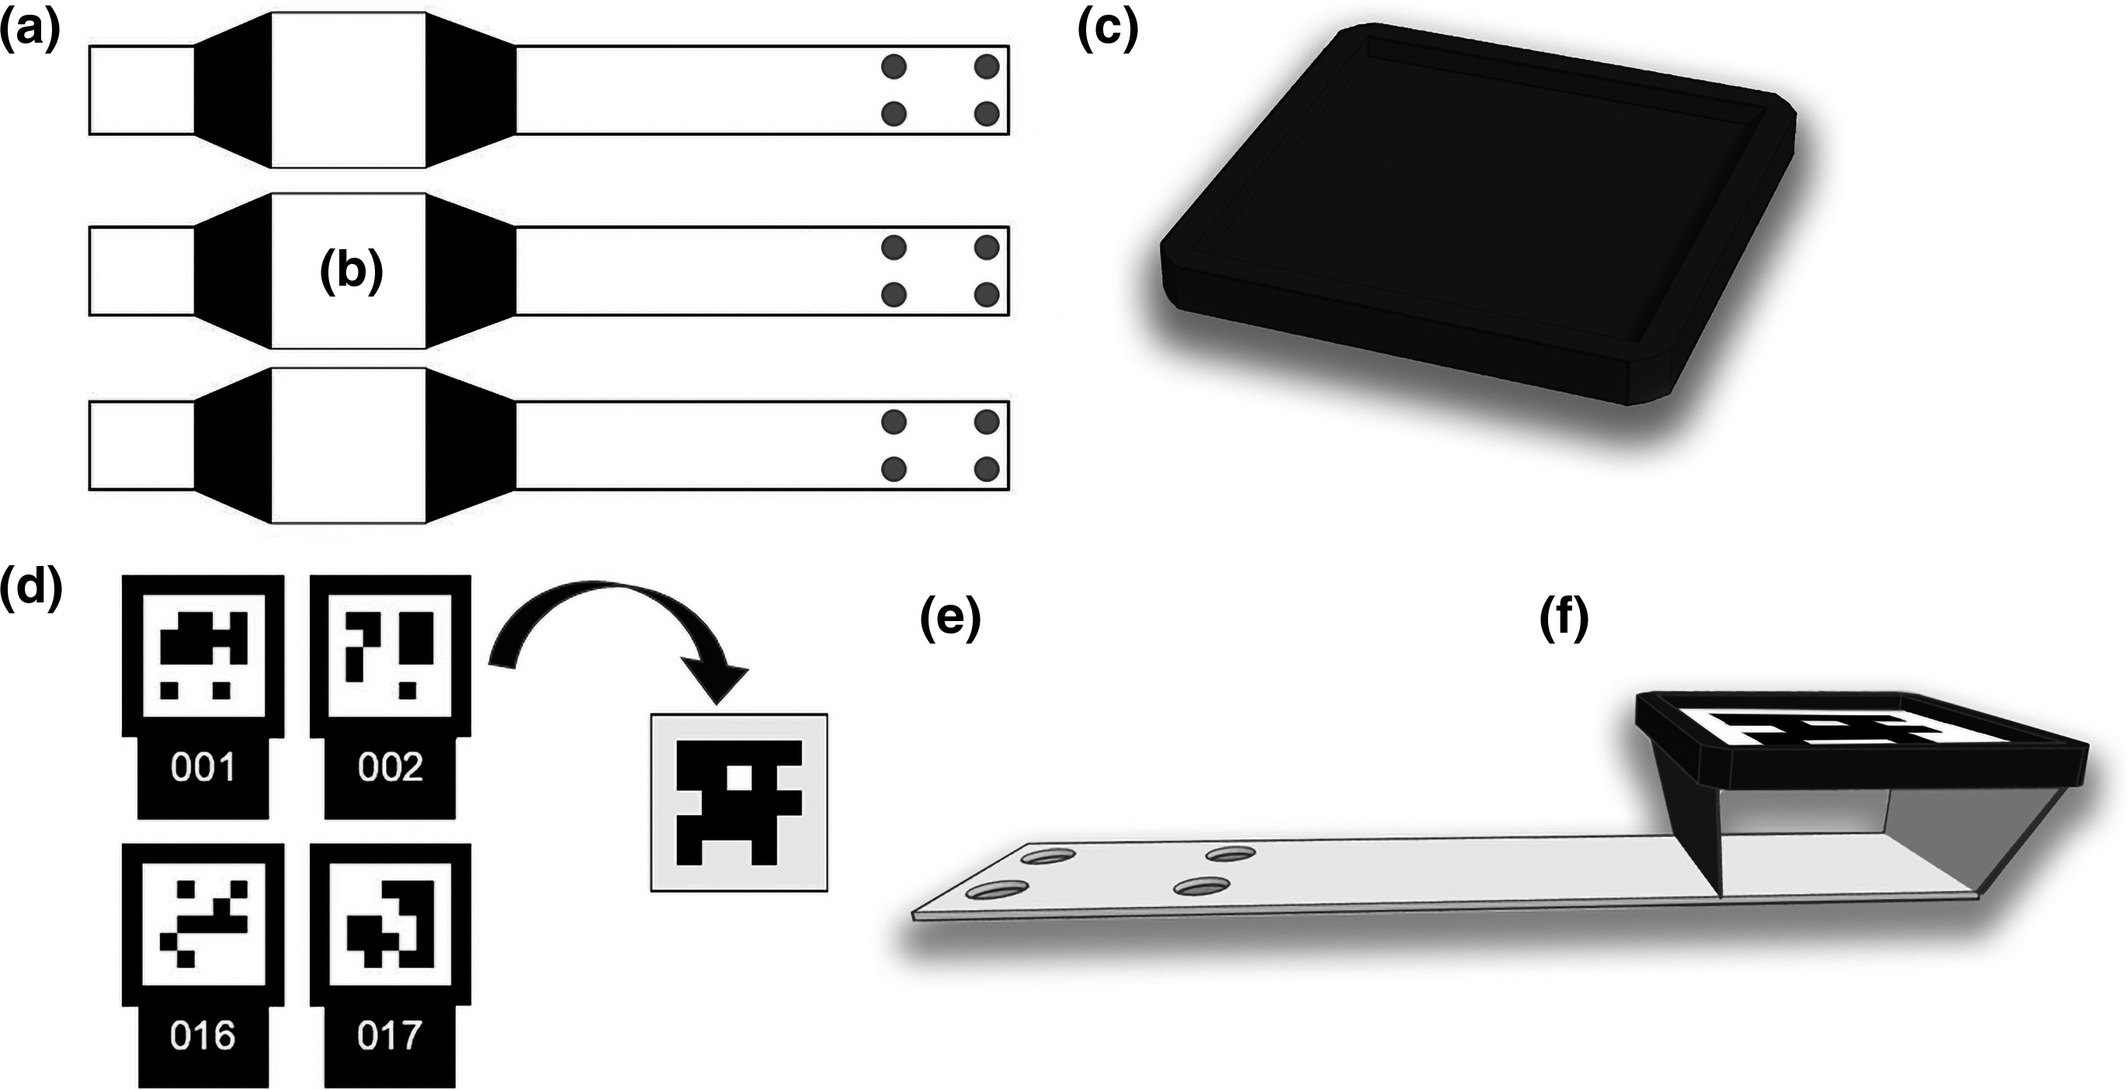
\includegraphics{Graving_IMPRS_Thesis/figures/bird_figure_1.jpg}
    \caption{Components and assembly of the backpack‐mounted barcodes. (a) Template layout. (b) Mount area where plastic trays (c) are glued. (d) Barcode layout and cutout to be glued on the tray. (e) Assembled backpack with tray and code raised on the mount (f)}
    \label{fig:bird_figure_1}
\end{figure}


Backpacks include a front strip of paper that fits between the scapulae of the bird, into which we punched four round holes (c. 1‐mm diameter, Figure \ref{fig:bird_figure_1}e) to attach the elastic string that formed the straps of the backpack around the bird (Figure \ref{fig:bird_figure_2}). For each backpack, we used a single piece of string 25‐cm long which we looped through the rear holes on the paper, crossed under the backpack, tied on the front holes, and kept the leads loose to allow for individual adjustment during deployment. For zebra finches, we used a 28 $\times$ 6‐mm front strip, a 10 $\times$ 10 mm mount raised 6 mm, and 10‐mm square tray. Backpacks weighed c. 0.27 g when fully assembled, including the straps.

\begin{figure}[!htb]
    \centering
    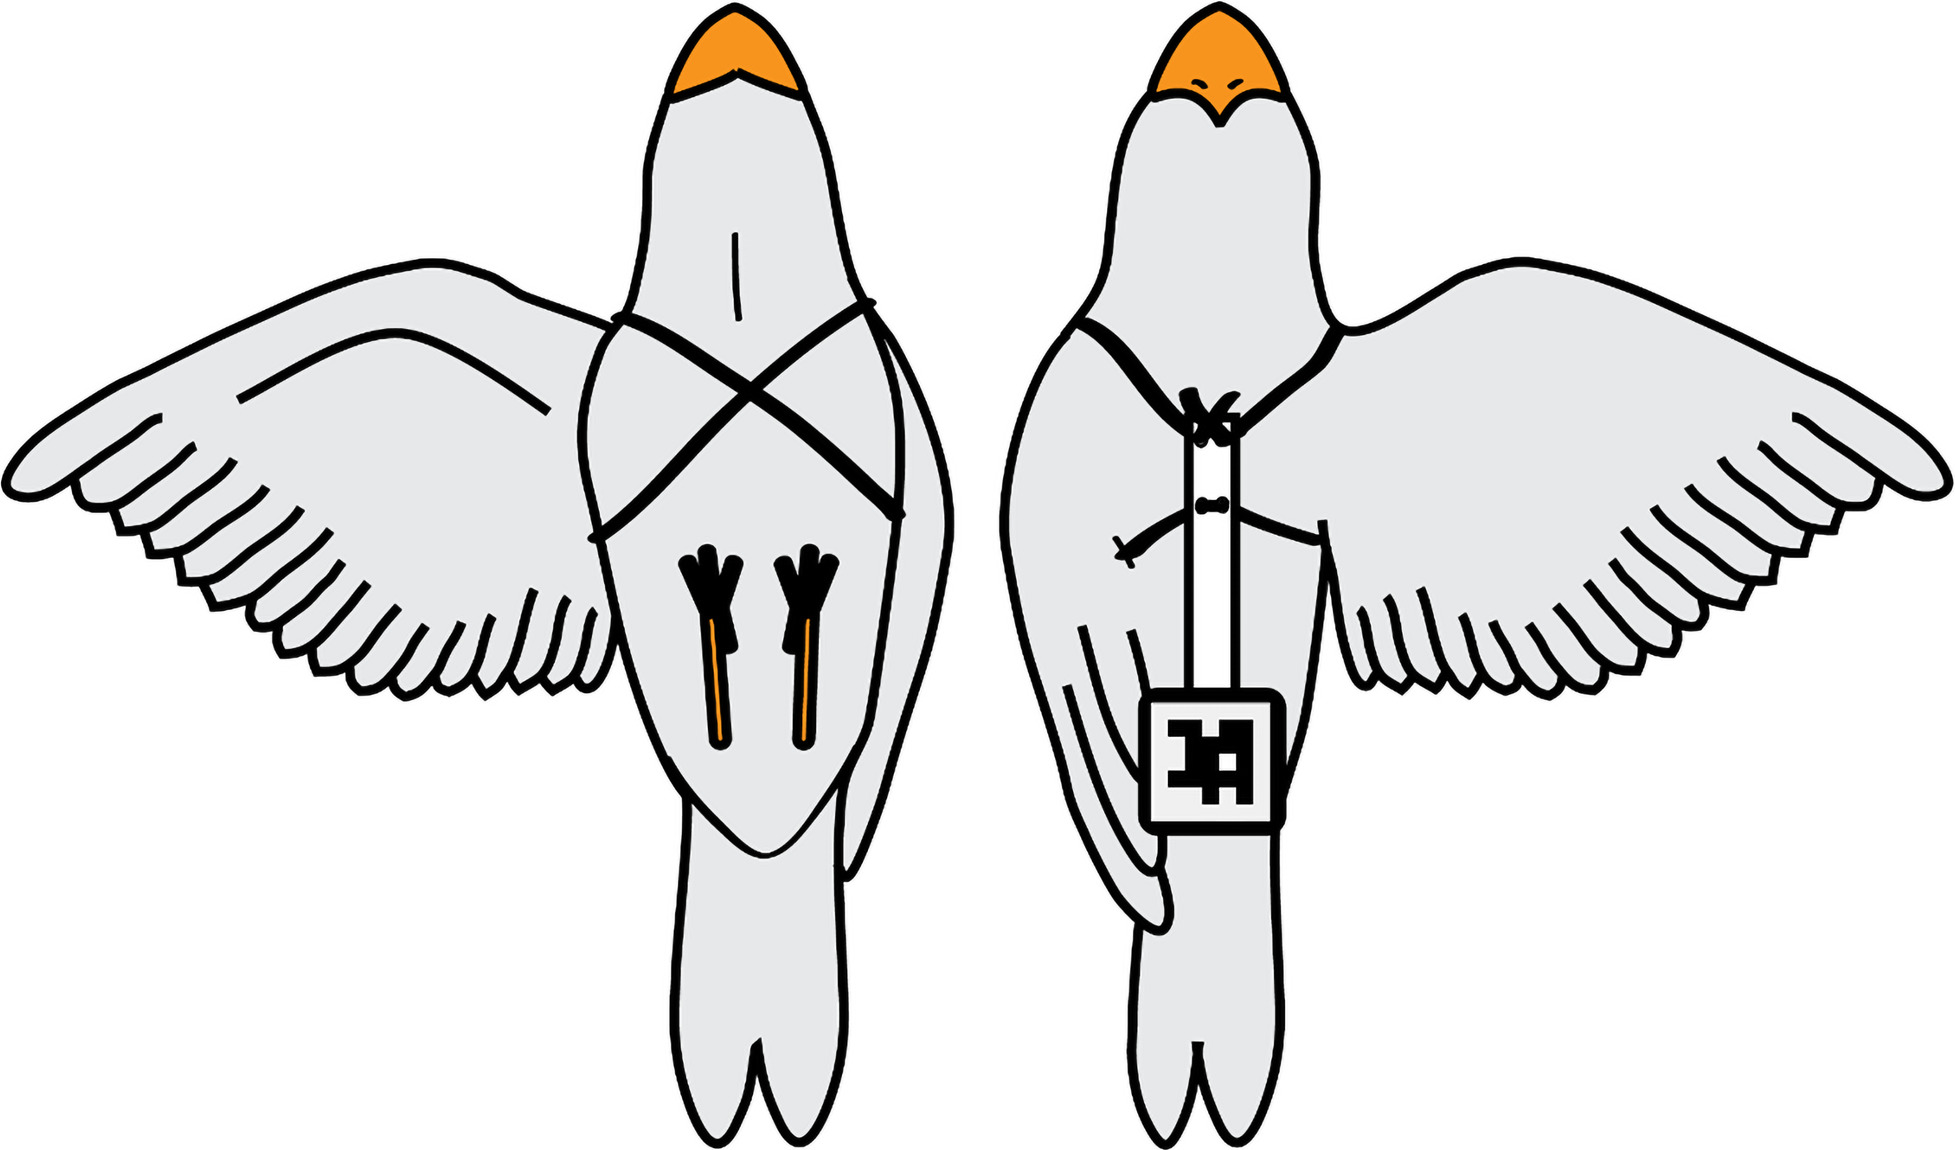
\includegraphics{Graving_IMPRS_Thesis/figures/bird_figure_2.jpg}
    \caption{Left: bottom view of bird with backpack. The string sits in front and behind the wings and crosses on the chest of the bird. Right: Top view. The string is tied at the anterior end of the backpack which goes between the scapulae, and the mount with the barcode sits on the rump, behind the wing joints}
    \label{fig:bird_figure_2}
\end{figure}
\subsubsection{Backpack deployment}
The general procedure for fitting backpacks includes the following steps: (1) Catching, measuring and recording health status of each bird; (2) Backpack fitting; (3) Observation during acclimation; (4) Releasing and monitoring birds in their permanent housing; and (5) Periodic health checks.

Once we confirmed the birds were in good health (step 1), we fit a completely assembled backpack to each bird (step 2). We pre‐tied the string on the backpack with a simple slipknot and then pulled the straps over the bird's head until the front strip sat on the interscapular area, carefully pulling each wing through the looped straps. We found that the best fit was achieved when the leading edge of the raised section was below the elbow joint of the wing, and the trailing edge was above the rump (Figure \ref{fig:bird_figure_2}). Once the backpack was in its final position, we tightened the string around the body, adjusting according to the size of each bird. The tightness must be firm enough to hold the backpack in position while preventing the bird to put its feet or toes inside of the loop, but also loose enough to allow the birds to fly and move freely, and to avoid blocking the crop. In their final position, the straps should sit midway between the body and the surface of the feathers. The front strip and the string loops eventually become covered by the feathers, while only the mount with the plastic tray and the barcode are visible. The mount must be positioned behind all the wing bones and joints, where only feathers can be in contact with it.

After fitting the backpacks, we placed subjects in a small observation cage (step 3) to monitor their behaviour. This step is critical for animal safety. We monitored birds for up to 1 hr until we were sure that they behaved normally, that is, with no observable hindering of movement. A well‐fitted backpack allows the animal to move freely, with no interference for flying, walking, landing or perching. Most birds tried to pull the backpacks or the straps off during this period. In our experience, the intensity and duration of this behaviour was not necessarily a signal of an ill‐fitting backpack and, on the contrary, preening helped to accommodate all the new elements. We found that the acclimation process worked better when subjects were kept in small groups (2–5) and in a separate room with no people present, as it reduced stress and allowed for allopreening, feeding and undisturbed movement. Once we considered the deployment procedure was successful, we made a final check of the adjustments, secured the knot near the neck of the bird a second small knot and cyanoacrylate glue, and cut any excess string from the leads. When necessary, we also trimmed some covert feathers around the mount to prevent any obstructions on the codes that might hinder detection.

Every time we observed a bird with hindered movement or unusual behaviour that could be related to the backpack (i.e. foot or toes trapped in a loose strap, incapable of flight, or unbalanced perching), we checked and readjusted the straps using blunt‐tip tweezers. In some cases, if a bird's movement did not improve after the adjustment, we completely removed the backpack, let the bird rest to reduce stress, and observed it without the backpack before trying another deployment. After a second attempt, a few birds (4 of 58) still showed suboptimal performance despite having a well‐fitted backpack and appearing to be in good health. Our testing suggests that fewer than 5\% of subjects will never acclimate to the backpacks.

\subsubsection{Backpack monitoring}
We monitored the birds regularly, either during our experiments or during care‐taking activities, and constantly looked for unusual behaviour. This monitoring is important to prevent injuries or detect early symptoms of health issues, either related to the backpacks or otherwise. In our experience, most of the signs that could suggest ill‐fitted tags occurred within the first 2 days of observation after deployment and were addressed promptly. Importantly, some issues were only detectable when birds were settled in their permanent housing environment where they could fly much more extensively. We also monitored the birds by assessing the tracking data to identify individuals that were outliers in the number of detections (suggesting they behaved differently to others). The main issue we found arose after release into large aviaries was the backpack rubbing on the body or wings of the bird. Symptoms of this included bald spots on wings or neck, reduced movement or difficulty flying. These were addressed immediately by ensuring the backpack mount (and tray) were correctly fitted (i.e. not crooked and positioned away from the wings). However, in some cases, when the problem persisted, we completely removed the backpack, let the bird rest, and observed its behaviour without the backpack.

\subsection{Camera systems}
Barcodes can be detected using either photos or video. The choice largely depends on the research question to be addressed, as well as the scale of data collection and its associated processing and storage requirements. In this section, we provide details on the necessary considerations for implementing a camera system, and details of our experience using several implementations, including high‐resolution photos and video from action cameras, computer‐controlled DSLR cameras and the programmable camera module for the Raspberry Pi. We also discuss the pros and cons of each system for different types of research questions.

\subsubsection{Code size and capture}
For adequate detection and recognition of individual birds in photos or videos, the size of the barcodes should be at least 20 pixels per side in the captured image data (Crall et al., 2015), but this can vary depending on tag design and camera hardware. Detectability of tags can be improved, using high‐resolution cameras, reducing the distances between the codes and the camera (either physically or by using zoom lenses), or increasing the physical size of the deployed tags (which is limited by the study organism). Other considerations such as lens distortion, sharpness, and depth of field must be considered depending on the setup and area being captured. Lens distortion can be partially corrected via software, but this correction reduces the effective resolution of the images, especially for wide‐angle lenses (Figure \ref{fig:bird_figure_3}). Depth of field is an important consideration if the birds can perch at different heights, although issues can be avoided by having all perches on the same plane. Finally, the camera shutter speed needs to be chosen carefully. Slow shutter speeds result in blurred or overexposed codes and, thus, failed detections. To prevent these problems, exposure time should be set as short as possible while ensuring that contrast and noise levels are adequate for the software to successfully read the codes. We found that darker images had greater detectability as they increased the clarity of the edges within the barcodes by reducing bleeding of the white areas of the barcode into the black areas.

\begin{figure}[!htb]
    \centering
    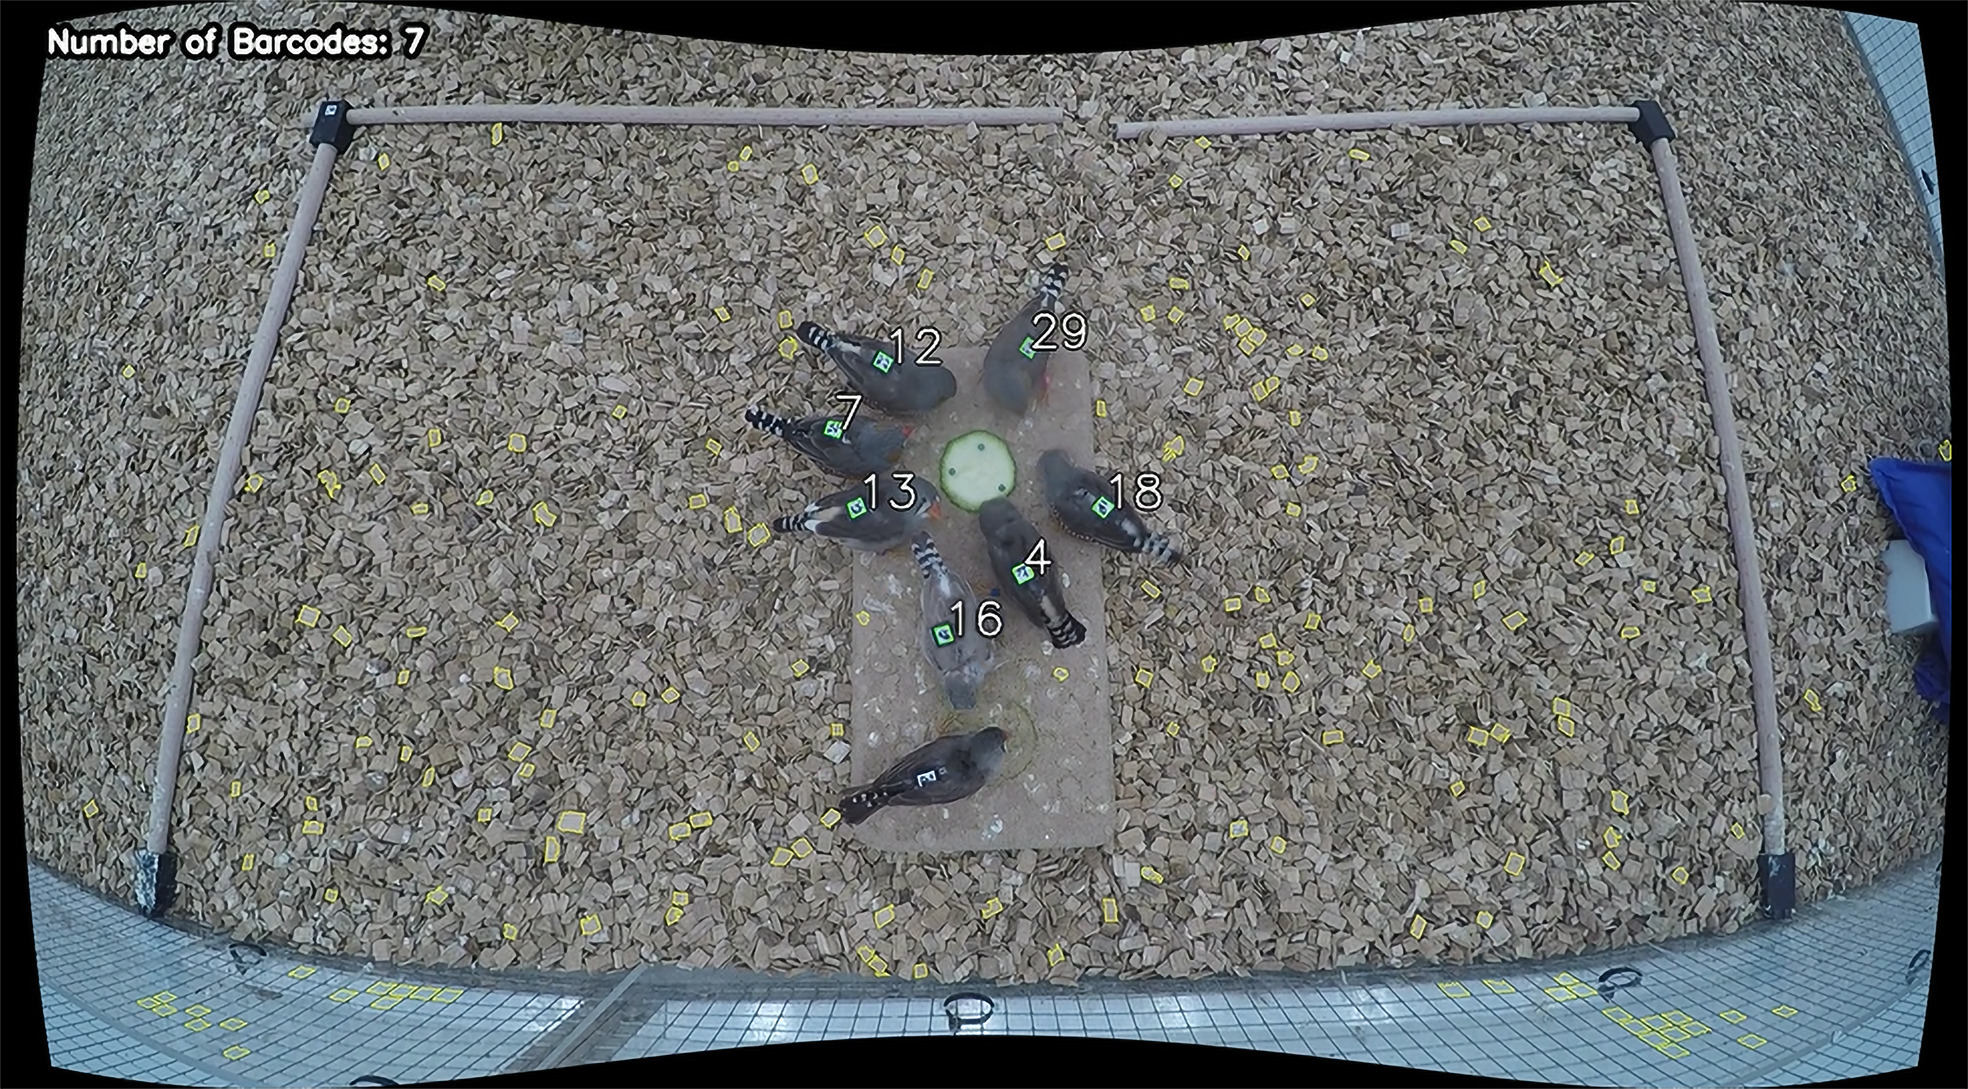
\includegraphics{Graving_IMPRS_Thesis/figures/bird_figure_3.jpg}
    \caption{Barcode detections in a feeding context in one video frame (from a GoPro camera). The food source in the centre of the arena was pinned to a wooden board to prevent birds from moving it out of the frame. The tracking algorithm detected barcodes on the back of each individual despite being on a complex background (wood chips). The yellow polygons are objects that were detected as candidate barcodes but did not match any known identities. The bird near the bottom of the image was not detected because its wings covered the barcode in this frame. Individual 16 was oriented away from the food. The black edges around image illustrate the software correction we used to partially compensate for wide‐angle lens distortion
}
    \label{fig:bird_figure_3}
\end{figure}

\subsubsection{Photos or video?}
Imaging technology requires a trade‐off between spatial and temporal resolution as hardware is always limited in its capacity to transmit and process signals. The choice between using photos or videos when capturing image data depends on the spatial or temporal resolution required to answer the research question. Video offers higher temporal resolution (typically ≥24 Hz) at the expense of spatial resolution (most hardware is limited to 3,840 $\times$ 2,160‐pixels), making it more suitable for studying behaviours that occur over short periods of time and in confined areas (e.g. allopreening, aggressive interactions, mating displays or copulation). Photos offer increased spatial resolution ($>$50 megapixels for some DSLR models) at the cost of temporal resolution (most cameras are limited to $<$15 Hz at full resolution), making them ideal for assessing behaviours in larger, open areas that do not require high‐frequency measurements (e.g. feeding, bathing, co‐perching, co‐feeding, etc.) and for quantifying associations over longer timescales (i.e. social networks, pair formation, etc.). Current imaging technologies vary widely in frame rate, image resolution, and file sizes, and different camera setups can be adapted for data collection depending on the research question and project budget. We implemented and tested three types of recording devices.

\subsubsection{Action cameras}
We used GoPro Hero 4 action cameras to record video of the birds in a feeding arena 90 $\times$ 50 cm on the floor of the aviaries (Figure \ref{fig:bird_figure_3}). We set the cameras to run continuously until the battery was depleted (c. 45 min) and chose a resolution of 1,920 $\times$ 1,080 pixels (1,080p) at 24 Hz to limit file size, reduce processing time, maximize battery life, and prevent the camera from overheating. We created a 3D‐printed arm to attach the camera to the side of the cage, 50 cm above the feeding arena and manually started recordings immediately after providing birds with a high‐value food patch (to attract them to this focal area of the camera).

These cameras produced adequate image quality but had noticeable distortion due to the wide‐angle fixed lenses. We manipulated the resulting images to reduce distortion before running the detection code (see “extracting data from images”). At 1,080p, we observed that the codes were sharp enough for detection, although at 24 Hz some frames suffer from image blurriness when birds moved. At 1,080p resolution, we generated a 4‐GB file every 15–17 min of video, which is the maximum file size supported by the cameras. This means that in a 45‐min recording session, we had to process three videos and store at least 12 GB. Limitations of this setup include the need to manually operate the cameras, restricted recording time due to battery life or large file size, and limited options for automating the entire system. Some of these problems, such as limited storage, lens distortion, and lack of automation, have been mitigated in newer models of the GoPro Hero series, as well as other brands of action cameras.

\subsubsection{Digital SLR cameras}
We briefly tested data collection using four Canon EOS1200 DSLR Cameras with 18–55 mm lenses for recording video or still images. We connected these cameras to Raspberry Pi 3 single‐board computers to control the image capture frequency. We placed the cameras at the top of the aviaries facing directly down. The cameras were set to capture one image at 1/200‐s every 10 min to measure the position of birds sitting on perches made from natural branches. These cameras can deliver high quality images up to 5,184 $\times$ 3,456 pixels (18 megapixels) and the zoom lenses allow for easy accommodation to different distances and to cover either small or large areas. However, this model had a loud mechanical shutter, which visibly disturbed the birds in the enclosed aviary space. Rather than modifying or removing the shutters, we abandoned this setup in favour of cameras with electronic shutters and no moving parts. In video mode, DSLR cameras can record high‐resolution video (1,080p) which is sufficient for collecting detailed movement data. Unfortunately, the recording time for many models is limited to 30 min.

\subsubsection{Single-board computers with camera}
We used Raspberry Pi 3 Model Bs (Raspberry Pi Foundation), each fitted with an 8‐megapixel Camera Module V2 (RS Components Ltd and Allied Electronics Inc.), to record photos of birds on perches (Figure \ref{fig:bird_figure_4}). We installed two of these on top of each aviary, covering most of the perch system without overlap. To record the birds present, we set the system to capture one image every 10 s, from dawn to dusk. In our experience, one of the most important advantages of this system is the possibility of programming automation scripts via the picamera software package (Jones, 2013) for Python (Python Software Foundation, available at http://www.python.org). This approach gives the user fine‐scale control over the quantity, sampling frequency, and spatial resolution of photos and videos. In combination with standard networking protocols like Secure Shell, these features allow for a fully automated pipeline that includes image capture, with file transfer, processing, and data storage when networked to a more powerful host computer. Another important advantage of these computers is their low cost, especially if the system requires multiple cameras per aviary or across multiple replicas in an experimental setup. Among the disadvantages of this system is the inconsistent quality of the camera modules (a small proportion of our cameras were unable to produce sharp images). To deal with this, we tested the cameras on the experimental setup and avoided using those that seemed to be defective. Although these camera modules provide a large depth of field, they require manual focusing, which can be difficult and is often inconvenient (Table 1).

\begin{figure}[!htb]
    \centering
    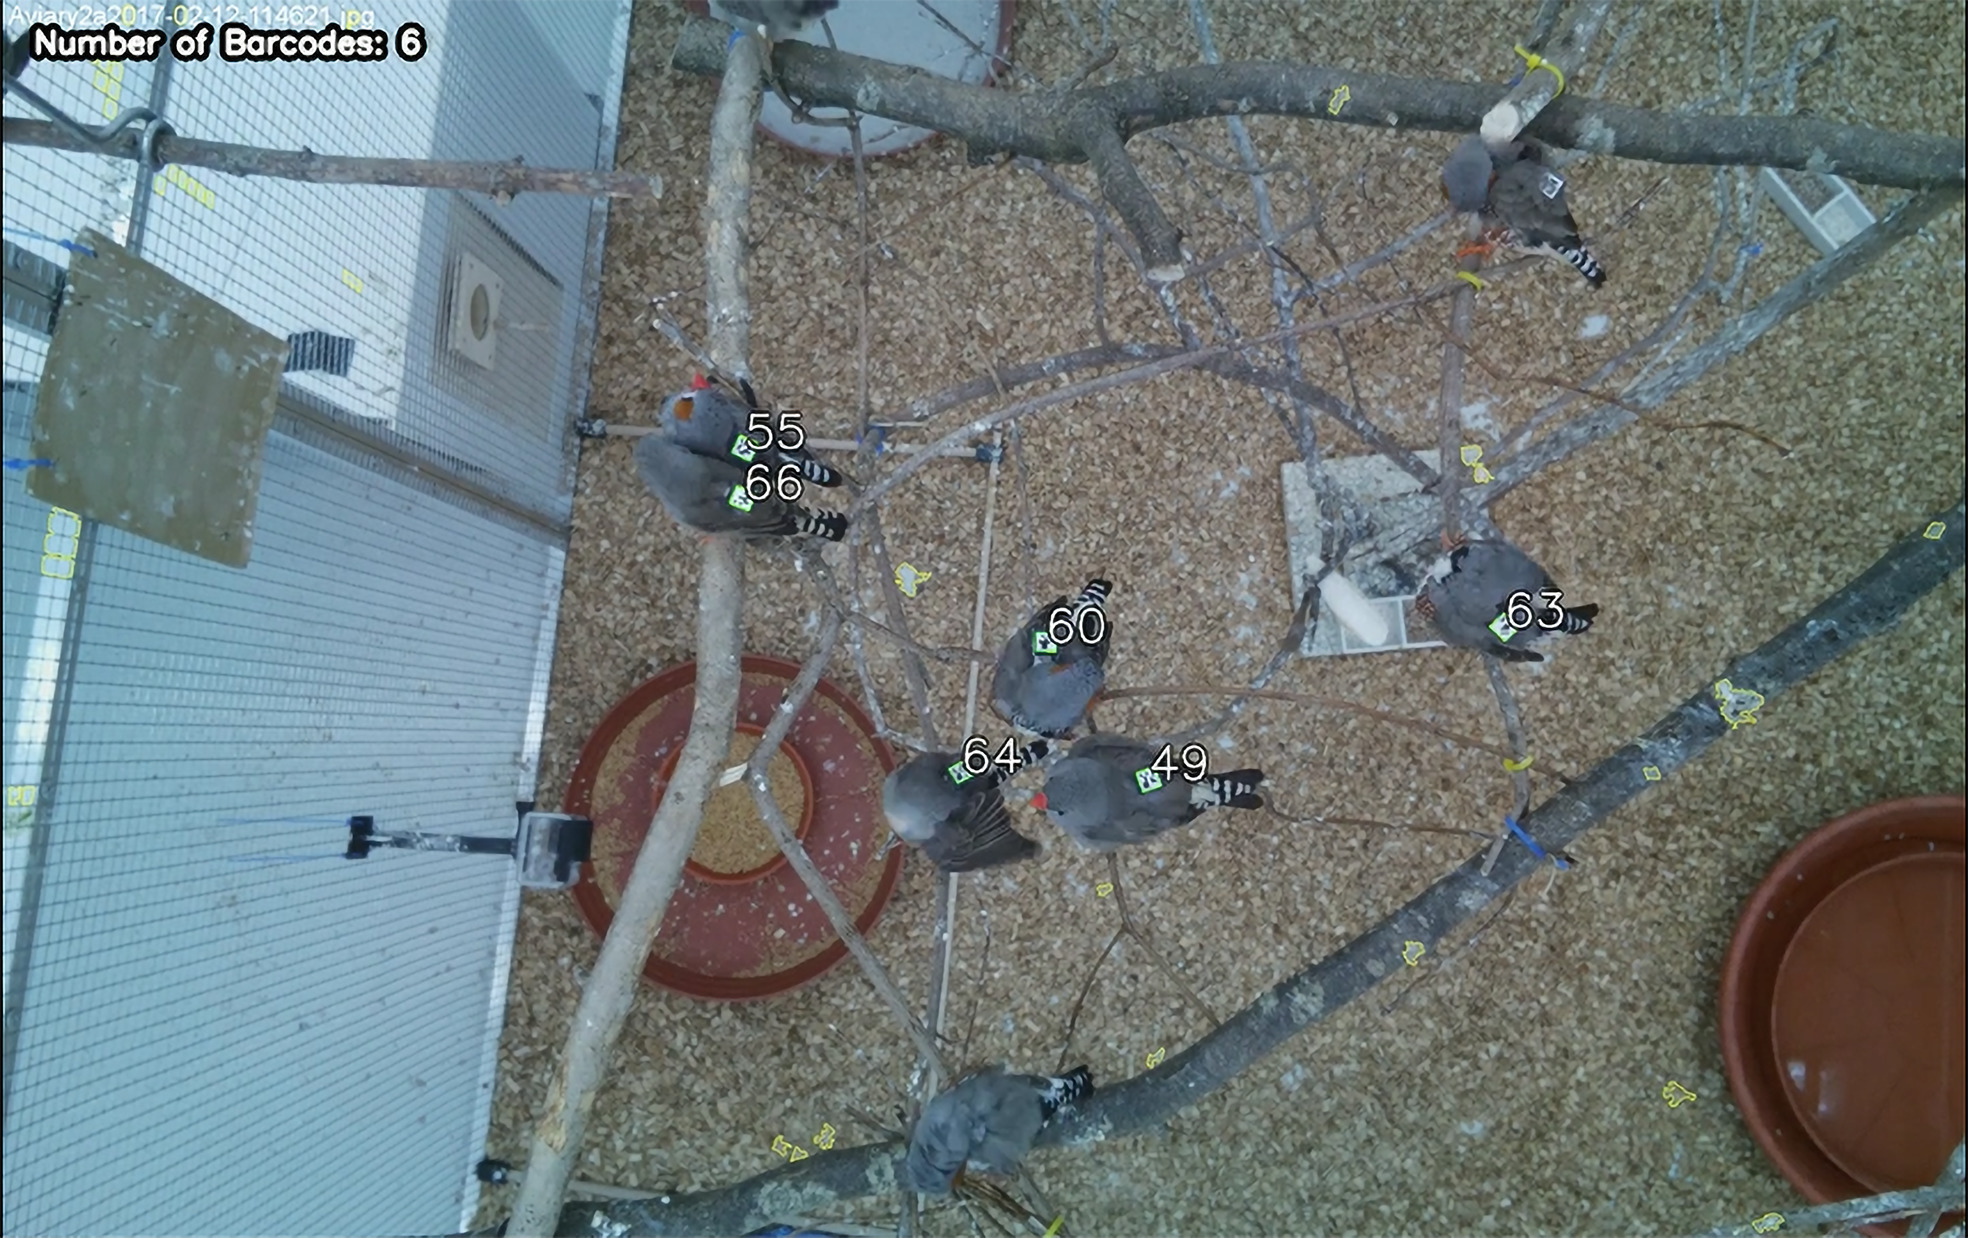
\includegraphics{Graving_IMPRS_Thesis/figures/bird_figure_4.jpg}
    \caption{Barcode detections in a social perching context (photographed with the Raspberry Pi camera module). The software can easily detect visible codes in complex aviary environments and extract information about important interactions, such as direct body contact (individuals 55 and 66), that many tracking algorithms would fail to detect
}
    \label{fig:bird_figure_4}
\end{figure}
\begin{table}[!htb]
\caption{Summary of the pros and cons of different camera implementations tested}
    \begin{tabular}{| m{0.2\textwidth} | m{0.4\textwidth} | m{0.4\textwidth} |}
    \hline
         \textbf{Camera system} & \textbf{Advantages} & \textbf{Disadvantages} \\ \hline
         DSLR (Canon EOS 1200)	& Image quality. Availability of lenses and accessories. Suitable for video or photo. Low‐light performance.	& Noisy mechanical shutter (this model). Video limited to 30 min. Bulky. Costly. \\ \hline
         Action Cameras (GoPro Hero 4)	& Compact size. Image resolution and quality. Suitable for video or photo. Wide angle lens suitable for small spaces.	& Lens distortion. Limited battery life. No display (this model). Manual operation (this model). \\ \hline
         Single‐board computers/Camera module (Raspberry Pi 3 Model B with Camera V2)	&
         Inexpensive. Compact size. Suitable for video or photo. Programmable. Network access. Expected improvements and software updates. No battery life limitation.	& Lower image quality. Fixed recording area. Difficult manual focusing. \\
         \hline
    \end{tabular}
\label{table:bird_table}
\end{table}

\subsection{Extracting data from videos and images}
Once videos or images are recorded, the next step is to extract location data from the barcodes contained in the image data. Several software libraries are available to accomplish this (Crall et al., 2015; Garrido‐Jurado, Muñoz‐Salinas, Madrid‐Cuevas, \& Marín‐Jiménez, 2016; Graving 2017; Wang & Olson, 2016), and each provides its own set of barcodes. These software libraries all extract the identity, location, and orientation of each tag from image data. In our study, we used the software library pinpoint by (Graving 2017), which is a based on the work of Garrido‐Jurado et al. (2016).

\subsubsection{Code detection}
The detection algorithm finds the identity matrix of the barcode using the contrasting white and black edges between the barcode and the black frame of the plastic tray on the backpack. Images are binarized using an adaptive (spatially localized) thresholding algorithm, which allows for uneven lighting, and candidate barcodes are detected based on their geometry, which allows for complex backgrounds. Once a candidate barcode is detected, the identity matrix is extracted from the pixel data and compared to known identities stored in a tag dictionary. The tracking algorithm can reliably detect the codes at arbitrary angles, even when they are not completely perpendicular to the central‐axis of the camera lens. The software provides the identity and Cartesian coordinates for the corners of each detected barcode with sub‐pixel resolution, which can be used to calculate the orientation of the code (note the importance of fitting the code in the right direction on the birds).

\subsection{Example data analyses}
To briefly demonstrate the use of this automated approach to data collection and analysis, we studied the foraging behaviour of individual zebra finches at a high‐quality food source and constructed foraging networks based on high‐resolution movement data measured using our system. Social networks are particularly challenging to study using manual observation because they require measuring the behaviour of most or all individuals simultaneously. To achieve this, we created an arena 90 $\times$ 50 cm on the floor of each of the two aviaries and provided birds with an ephemeral high‐quality food resource (a slice of zucchini/courgette) twice per day (around 9.00 and 16.00 hr). We used a barcode to record the centroid of the resource, which was subsequently removed to allow birds unobstructed access to food. Birds were fasted for an hour before the experiment to ensure they were motivated to feed, and their access to the food resource was captured on video using the GoPro Hero 4 camera fitted 50 cm above the food (see above). We collected data on the two aviaries for 58 days, between December 15, 2016 and March 29, 2017.

We extracted feeding association data, representing the propensity for individuals to synchronize their feeding and tolerate one another at the food source. We recorded the identity of individuals detected at the food for every video frame by defining a feeding zone with respect to the centroid of the food resource. A feeding event was recorded when a barcode was detected within a 154‐pixel (or c. 8‐cm) radius of the resource centroid, and the bird was facing the food (i.e. the centroid was within the 180$\degree$ zone in front of the bird) (Figure \ref{fig:bird_figure_3}). Once we identified the individuals in every frame and classified feeding events, we constructed a weighted, undirected social network representing the co‐feeding relationships among individuals (represented as nodes) in each flock. We accomplished this by transforming our data into a matrix of pairwise associations using a simple ratio index ($\mathrm{SRI}$) for every pair of individuals in each flock (see Farine & Whitehead, 2015). Here, the edge weight between two individuals ($\mathrm{SRI}_{ij}$) is the probability of observing individuals $i$ and $j$ feeding together given that either $i$ or $j$ has been detected. This calculation is simply given by the following:
\begin{equation}
    \mathrm{SRI}_{ij} = \frac{x_{ij}}{n},
\end{equation}

for $i, j = 1, \dots, N$ and $i \neq j$, where $N$ is the total number of individuals in the flock, $x_{ij}$ is the number of frames in which individuals $i$ and $j$ were feeding together, and $n$ is the total number of frames where either $i$ or $j$ was detected (alone or together).

\section{Results}
\subsection{Barcode deployment and maintenance}
We deployed backpacks on 58 zebra finches (Figure \ref{fig:bird_figure_5}), which required about 3 min of handling per individual, plus observation and monitoring time. All the deployed backpacks lasted throughout the experimental period (4 months or more) without causing any injuries to the birds. However, minor maintenance was required as backpacks and codes showed some wearing due to grooming and allopreening (see backpack‐mount in Figure \ref{fig:bird_figure_5}). Common issues included loss of ink on and around the barcodes, weakened paper around the front holes, and unglued mounts. We also noticed that, in a few cases, the straps lost elasticity after 4 months and appeared loose. More commonly, we observed that debris (i.e. food remains or excrement) on the barcode obstructed its detection. Every time we detected one of these issues, we addressed it immediately to guarantee both safety of the birds and quality and continuity of the data collection. For any minor issues, we carefully cleaned the codes to remove debris, or covered the ink‐less spots with black ink permanent markers. For extensive damage on the mount or the surface of the barcode, we removed and replaced the mount keeping the strip and the elastic string on the bird, thus reducing manipulation and acclimation time. In cases that required a whole new backpack, we repeated the process of the first deployment.

\begin{figure}[!htb]
    \centering
    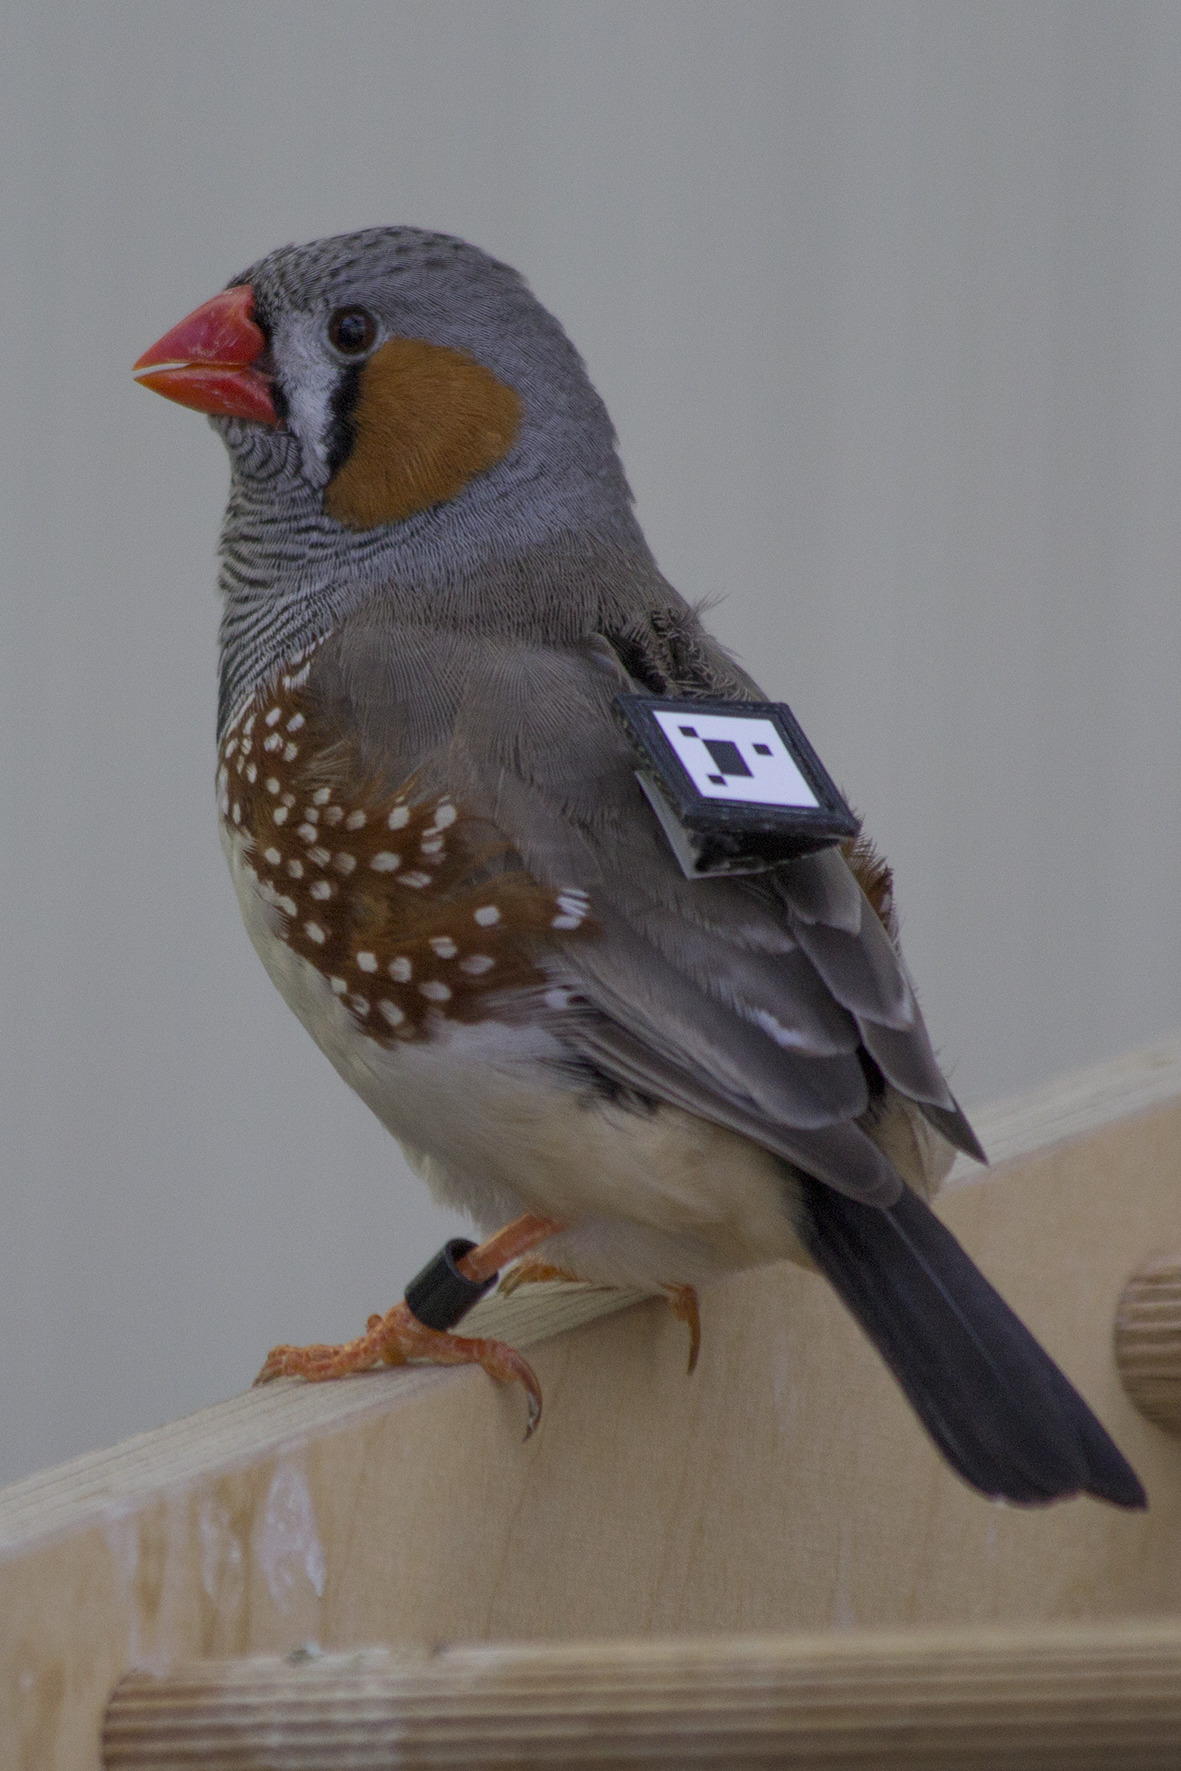
\includegraphics{Graving_IMPRS_Thesis/figures/bird_figure_5.jpg}
    \caption{Male zebra finch with a barcode backpack c. 4 months after fitting. Note the wearing on the backpack structure caused by grooming behaviours
}
    \label{fig:bird_figure_5}
\end{figure}

\subsection{Detection}
We recorded 48 hr of video at the feeding arenas using GoPro Cameras and recorded photos using Raspberry Pi cameras. The detection software identified 52.05\% of the barcodes (i.e. birds) present in 100 randomly selected frames from the GoPro footage. This percentage was improved to 64.58\% after simple linear interpolation of positions across short gaps of missing data (e.g. 1–24 frames of video). From the photos of birds perched on the aviary branch system, the software detected 60.4\% of the individuals present in 100 randomly sampled images captured, using the Raspberry Pi cameras. The most common reasons for failed‐detections were motion blur and feathers temporarily obscuring parts of the code (e.g. Figure \ref{fig:bird_figure_3}). Motion blur was most prominent in GoPro videos but is easily prevented in photos using shutter speeds of 1/1000‐s or faster (which can even identify birds in flight, Figure \ref{fig:bird_figure_6}). Trimming some feathers around the code during backpack deployment can increase the number of detections, although we expect the current rate of data collection to be sufficient for most applications and research questions.

\begin{figure}[!htb]
    \centering
    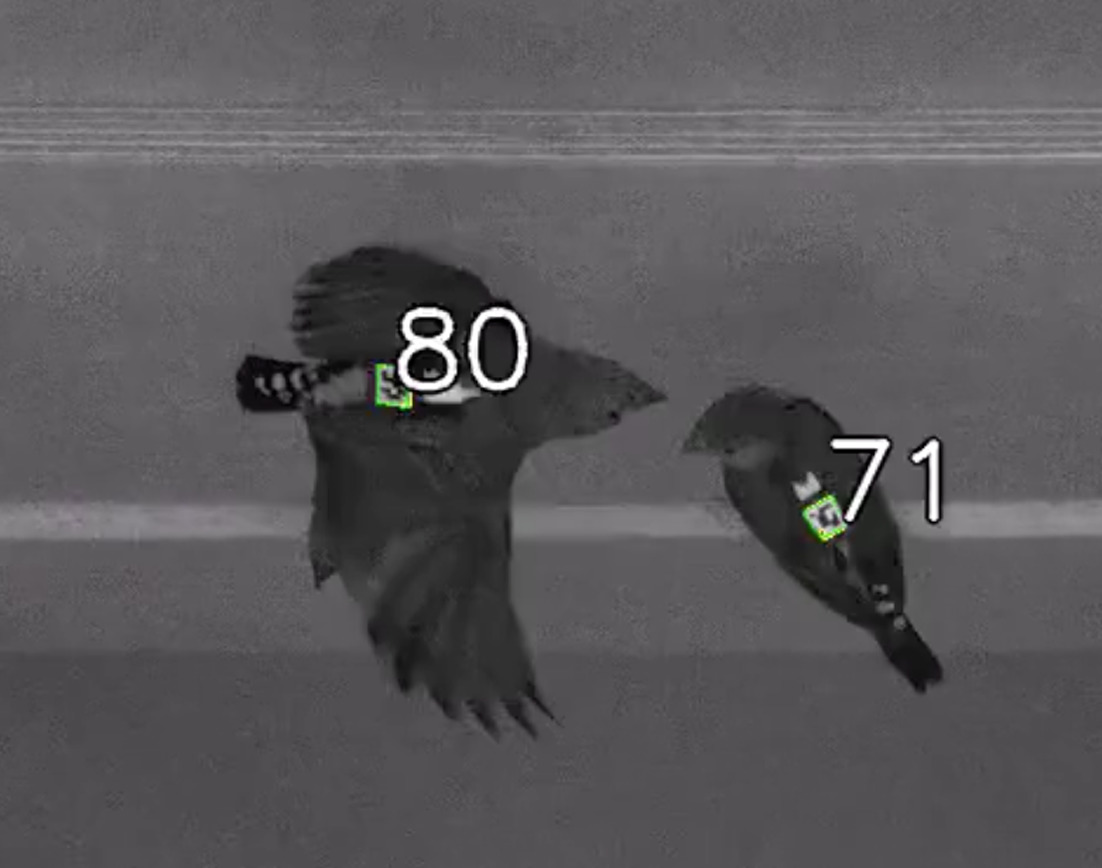
\includegraphics{Graving_IMPRS_Thesis/figures/bird_figure_6.jpg}
    \caption{Example of a zebra finch (individual 80) being detected in flight (with 1/2000‐s shutter speed)
}
    \label{fig:bird_figure_6}
\end{figure}
\subsection{Example data analyses}
Using image data collected with a GoPro mounted over the food arena, we were able to distinguish birds consuming the resource from those present in the frame but not feeding (Figure \ref{fig:bird_figure_7}). For example, from a single 45‐min observation period, as shown in Figure \ref{fig:bird_figure_7}, we recorded 74,960 records of individual positions. These records also contain many potential interactions. We demonstrate that the data on the co‐presence of individuals at a food source can be used to generate social networks (Figure \ref{fig:bird_figure_8}), a powerful approach used in many studies of animal behaviour for which extensive observation data are required.

\begin{figure}[!htb]
    \centering
    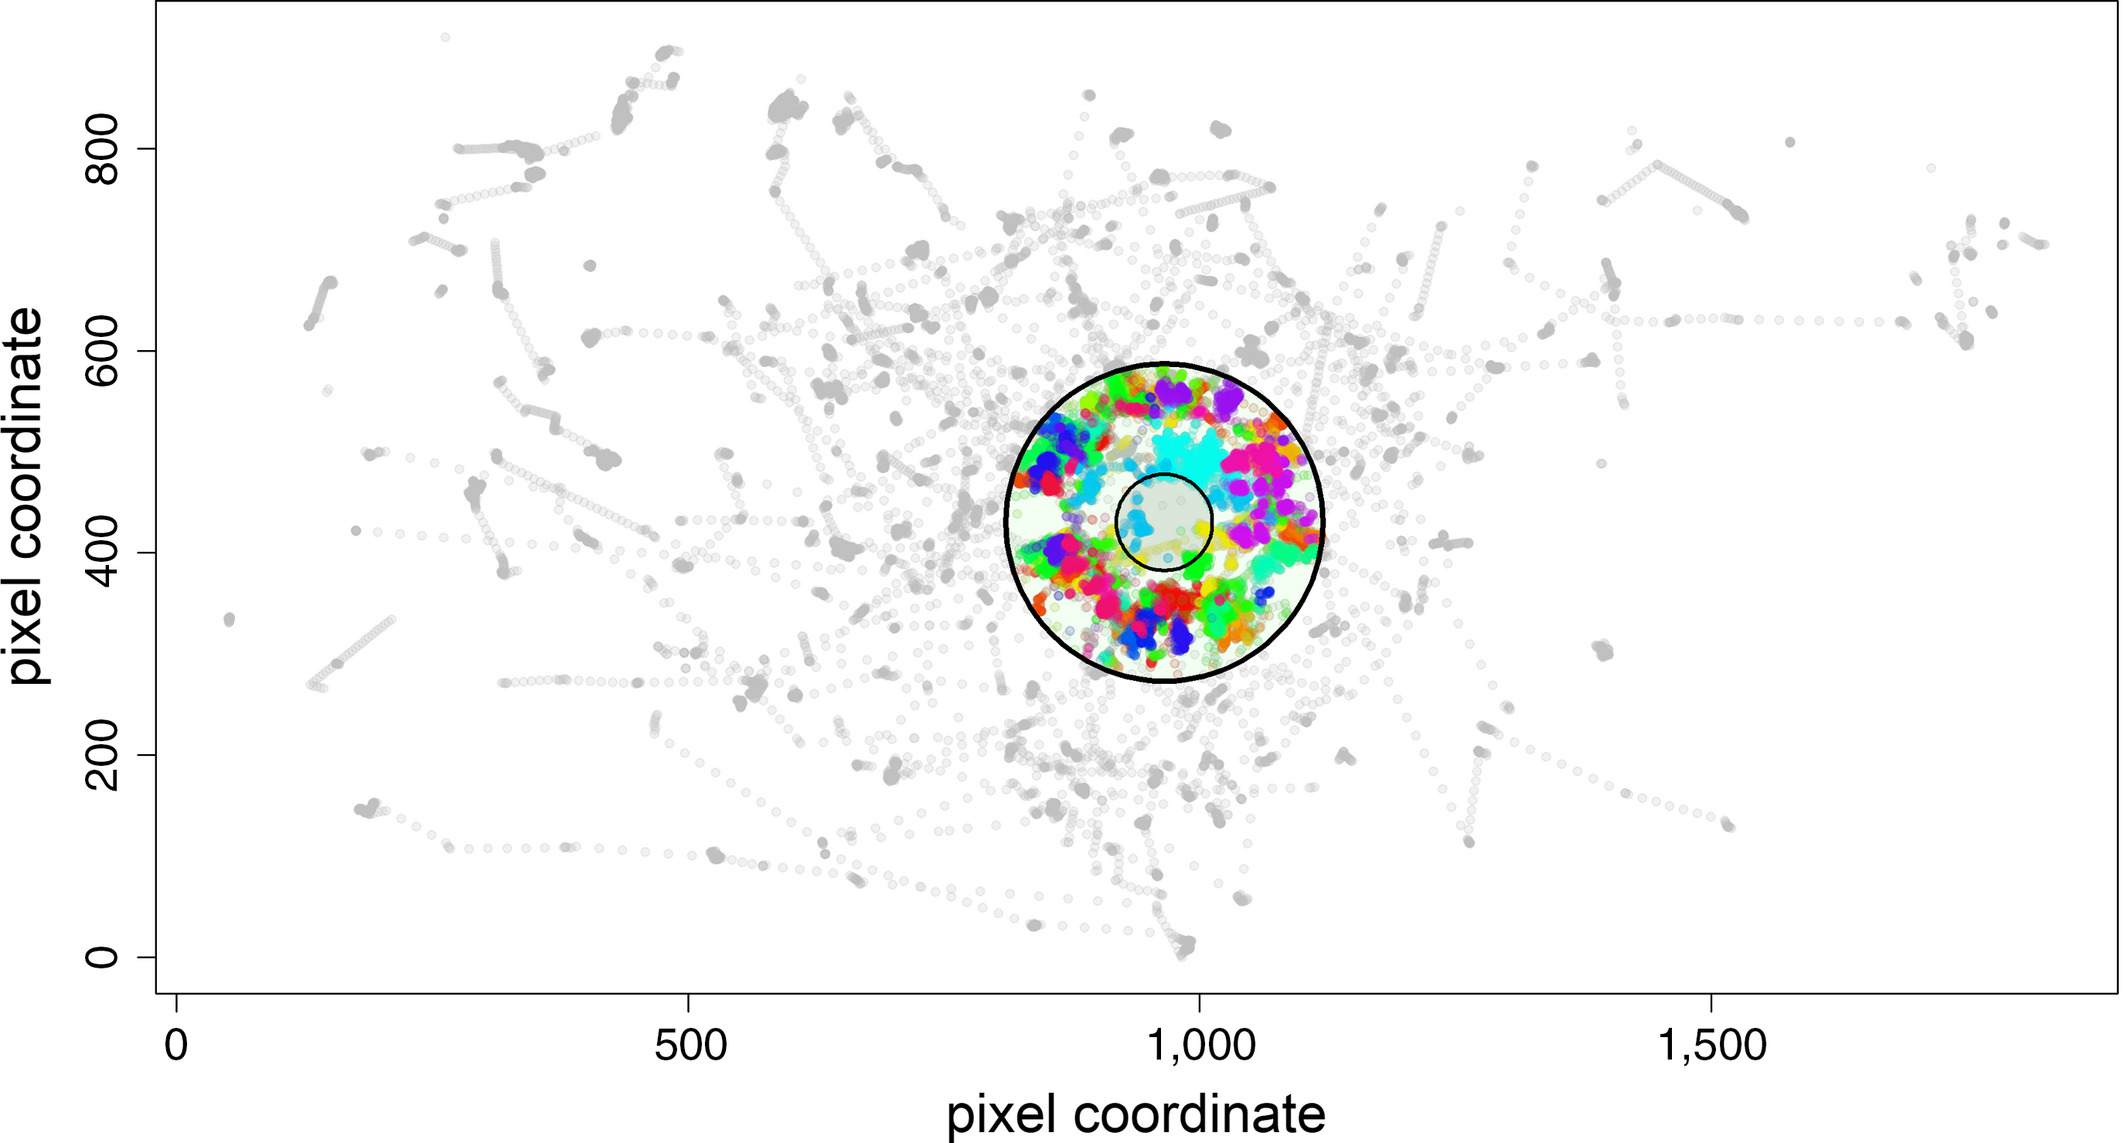
\includegraphics{Graving_IMPRS_Thesis/figures/bird_figure_7.jpg}
    \caption{Detection of feeding behaviour characterized by proximity and directionality to the food source. The inner circle represents the outline of the food source, and the outer circle represents the 154‐pixel boundary for birds to considered to be “at food.” Coloured dots represent detections of different individuals within the “at food” zone. Grey dots are birds present and identified in the frame but not actively feeding. The positions of birds away from the centre of the frame are less accurate due to lens distortion (see Figure \ref{fig:bird_figure_3})
}
    \label{fig:bird_figure_7}
\end{figure}

\begin{figure}[!htb]
    \centering
    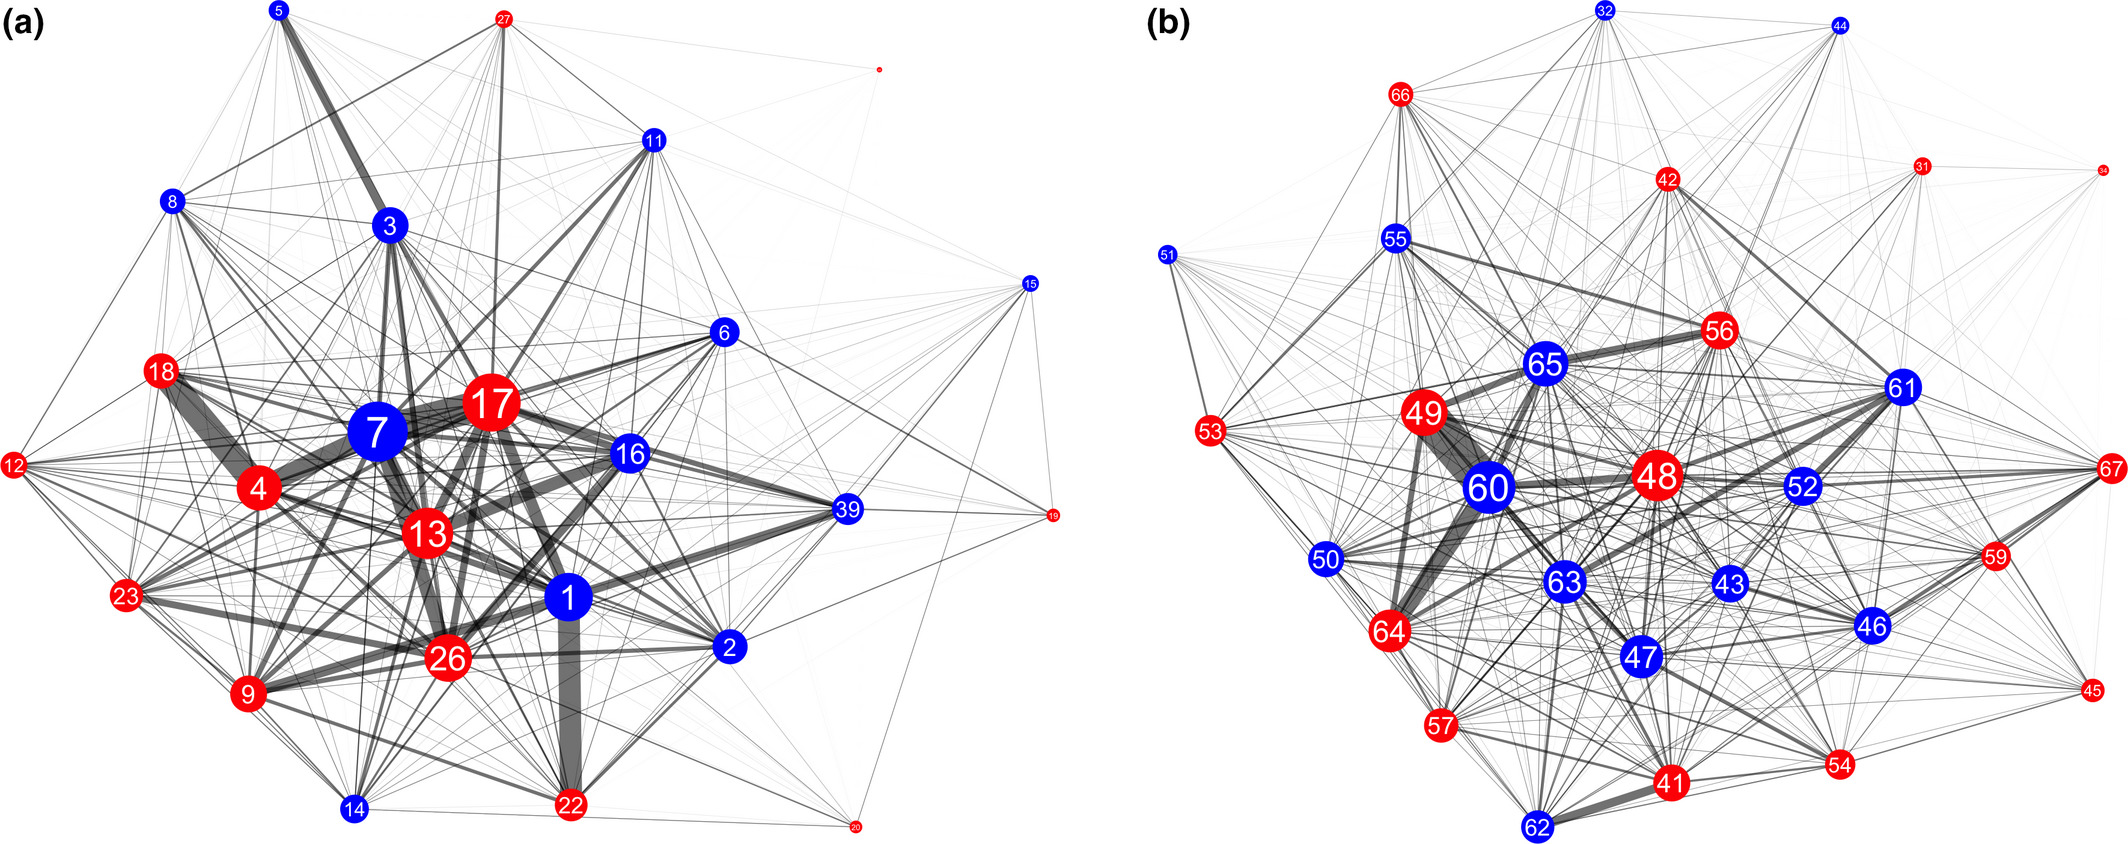
\includegraphics{Graving_IMPRS_Thesis/figures/bird_figure_8.jpg}
    \caption{Affiliative networks generated with co‐feeding data extracted from barcodes detected at a food source using a video camera in (a) flock 1 and (b) flock 2. Each node (circle) represents an individual. Red nodes represent males, and blue nodes represent females. The size of the node represents the individual's degree in the network, a measure of centrality computed by summing the weights of all the edges connected to it. The thickness of the line represents the strength of the association between each pair of individuals
}
    \label{fig:bird_figure_8}
\end{figure}

\section{Discussion}
We present a method for recording the behaviour of captive birds using backpack‐mounted barcodes, image capture, and computer detection. With proper deployment, manipulation and monitoring, we have shown that this system is safe for the birds, durable, and capable of delivering extensive data from multiple individuals simultaneously. These position and orientation data can be used to assess multiple types of behaviours, associations and interactions among individuals. This system presents several advantages to more commonly‐implemented methods. In particular, it is adaptable to different contexts and research questions, being possible to vary the temporal resolution (photos or video) and the area covered without requiring any additional markers to birds. For general purposes, the use of Raspberry Pi single‐board computers and camera modules makes this method affordable, enabling high‐throughput data collection that increases sample sizes and statistical power. Our example analyses demonstrate that the barcode‐based approach can generate similar data to what is often collected using PIT tags (Figure \ref{fig:bird_figure_8}), but also provides much richer information on movements and spatial location within patches (Figure \ref{fig:bird_figure_7}). We found that the backpack system simplified the data analysis because we were certain about the co‐occurrence of birds at the same food source (i.e. captured in the same frame), instead of having to infer co‐occurrences from sequences of detections using pattern‐recognition algorithms (e.g. Psorakis et al., 2015).

We tested the application of different camera setups and behavioural contexts, including video for feeding arenas and photos in co‐perching scenarios. Cameras could be fitted in various locations, including bathing areas, nest boxes, and potentially in open areas to capture birds in flight (e.g. Figure \ref{fig:bird_figure_6}). The decision on the type of camera and on video or photos will depend on each research question. For example, researchers could choose video for recording aggressive interactions or other behaviours that involve movement, or capture photos every few seconds to capture affiliative data for the purposes of studying social networks, pair formation, or group stability. The type of data provided by these barcodes also provides new opportunities for analysis. Using machine learning, it will be possible to automatically classify behaviours and interactions over extended periods of time while also minimizing manual annotation by a human observer (Robie, Seagraves, Egnor, \& Branson, 2017), thereby avoiding bias and fatigue. Such approaches have been developed for studying other organisms (Kabra, Robie, Rivera‐Alba, Branson, \& Branson, 2013), which use data that are similar to what our system generates.

Our backpack‐based barcode method has potential to be extended to diverse range of systems. Although we only collected data during daylight hours, barcodes could easily be detected in low‐light conditions and many commercially available infrared cameras can image the black‐and‐white codes without visible light (using infrared lights). While most birds are not very active at night, there is increasing evidence that many important behaviours happen early in the morning (Bonter, Zuckerberg, Sedgwick, \& Hochachka, 2013). Such behaviours could easily be captured with this barcode system but would be almost impossible to study using manual observations or video as it is difficult to identify coloured leg bands. Future applications include using barcodes to identify individuals interacting with a device (e.g. a feeder or a puzzle box). To date, such systems have mostly relied on using PIT tags (e.g. Aplin et al., 2015), which limits sampling to a single individual at once. In social species, individuals often congregate, and a barcode system can facilitate multiple simultaneous detections and quantify relative positions of individuals to one‐another and to the device. The implementation of “real‐time” detection could allow for algorithms that control devices in response to the behaviour of birds, such as allowing only a maximum number of individuals in one area or selectively dispensing food to particular individuals (as performed by Firth, Voelkl, Farine, \& Sheldon, 2015). Barcodes could provide a powerful interface between individuals and experimental devices, not only by being able to provide tailored responses (such as individual learning algorithms, Morand‐Ferron, Hamblin, Cole, Aplin, \& Quinn, 2015), but also, unlike almost any other system, by capturing information about who else is present when particular events occur.

Although we have discussed the multiple advantages, the limitations of the system must be also considered. While backpacks and barcodes can last for more than 4 months, permanent monitoring was required to assure safety of the birds and adequate delivery of data. Grooming and allopreening caused some wear on the backpacks and codes, and this sometimes led to impaired movement of the birds. Detecting and addressing such issues is important for both safety of the birds and continuity of the data collection. Additionally, there are unavoidable issues that reduce detectability, like fast movement, codes tilted due to extreme body position, and wings or feathers partially covering the trays. The current design of the backpacks addresses these issues well and delivers consistent detection. Additional concerns related to camera systems, such as storage, resolution, lens distortion or lighting, can be solved for specific research circumstances.

A key question that requires further investigation is whether these backpacks will be suitable for field deployment. We found that, in zebra finches, we could detect most issues within the first 1–2 days. However, few field studies are amenable to keeping birds in captivity to allow such monitoring. Thus, field applications may be limited to species that either have well‐established protocols for fitting backpacks in the field or those in which individuals can be easily monitored (e.g. territorial species). We believe that there is a danger that small songbirds could entangle their backpacks in small branches, particularly if backpacks become loose over time. Finally, our aviaries had artificial lighting that remained constant during daytime. Researchers conducting outdoor studies, with natural lighting conditions, must consider the changing environment (i.e. sun position and cloud coverage) to avoid unusable images due to the differences in light quality from dawn/dusk to noon. For example, sun shining directly on the white tag will make the code invisible to the camera, while a setup designed for sunny conditions would create completely black photos under cloudy conditions. The use of infra‐red cameras and infra‐red lighting is one way to overcome this challenge.

Our backpack‐mounted barcode system could revolutionize data collection in a range of experimental systems. We have demonstrated that it can be implemented safely and cheaply. Further, it has the ability to collect extensive data across many individuals simultaneously and the flexibility to address diverse research questions. With simple software modifications, the system can also be integrated into active devices that interface directly with individuals, which will prove to be an extremely powerful experimental approach.

\section{Data availability}
The raw tracking data files, including the distance from the food patch, that are used for the example data analyses can be found at https://doi.org/10.17617/3.19.




\newpage 
	\chapter[DeepPoseKit]{DeepPoseKit, a software toolkit for fast and robust animal pose estimation using deep learning \blfootnote{\textbf{Adapted from:} Graving, J. M., Chae, D., Naik, H., Li, L., Koger, B., Costelloe, B. R., & Couzin, I. D. (2019). DeepPoseKit, a software toolkit for fast and robust animal pose estimation using deep learning. eLife, 8, e47994 under a CC-BY-4.0 International License  \ccby} \\ \vspace{10mm} \Large Jacob M. Graving, Daniel Chae, Hemal Naik, Liang Li, Benjamin Koger, Blair R. Costelloe, and Iain D. Couzin}
	
	\normalsize
	\section{Abstract}

    Quantitative behavioral measurements are important for answering questions across scientific disciplines---from neuroscience to ecology. State-of-the-art deep-learning methods offer major advances in data quality and detail by allowing researchers to automatically estimate locations of an animal's body parts directly from images or videos. However, currently-available animal pose estimation methods have limitations in speed and robustness. Here we introduce a new easy-to-use software toolkit, \textit{DeepPoseKit}, that addresses these problems using an efficient multi-scale deep-learning model, called \textit{Stacked DenseNet}, and a fast GPU-based peak-detection algorithm for estimating keypoint locations with subpixel precision. These advances improve processing speed >2$\times$ with no loss in accuracy compared to currently-available methods. We demonstrate the versatility of our methods with multiple challenging animal pose estimation tasks in laboratory and field settings---including groups of interacting individuals. Our work reduces barriers to using advanced tools for measuring behavior and has broad applicability across the behavioral sciences.


\section{Introduction}
Understanding the relationships between individual behavior, brain activity (reviewed by \citealt{krakauer2017neuroscience}), and collective and social behaviors \citep{rosenthal2015revealing,strandburg2013visual, jolles2017consistent, klibaite2017unsupervised, klibaite2019interacting} is a central goal of the behavioral sciences—a field that spans disciplines from neuroscience to psychology, ecology, and genetics. Measuring and modelling behavior is key to understanding these multiple scales of complexity, and, with this goal in mind, researchers in the behavioral sciences have begun to integrate theory and methods from physics, computer science, and mathematics \citep{anderson2014toward, berman2018measuring, brown2018ethology}. A cornerstone of this interdisciplinary revolution is the use of state-of-the-art computational tools, such as computer vision algorithms, to automatically measure locomotion and body posture \citep{dell2014automated}. Such a rich description of animal movement then allows for modeling, from first principles, the full behavioral repertoire of animals \citep{stephens2011emergence, berman2014mapping, berman2016predictability, wiltschko2015mapping, johnson2016composing, todd2017systematic, klibaite2017unsupervised, markowitz2018striatum, klibaite2019interacting,Costa1501}. Tools for automatically measuring animal movement represent a vital first step toward developing unified theories of behavior across scales \citep{berman2018measuring, brown2018ethology}. Therefore, technical factors like scalability, robustness, and usability are issues of critical importance, especially as researchers across disciplines begin to increasingly rely on these methods.


Two of the latest contributions to the growing toolbox for quantitative behavioral analysis are from \cite{mathis2018deeplabcut} and \cite{pereira2019fast}, who make use of a popular type of machine learning model called \textit{convolutional neural networks}, or \textit{CNNs} (\citealt{lecun2015deep}; Appendix \ref{app:cnn}), to automatically measure detailed representations of animal posture—structural \textit{keypoints}, or \textit{joints}, on the animal's body—directly from images and without markers. While these methods offer a major advance over conventional methods with regard to data quality and detail, they have disadvantages in terms of speed and robustness, which may limit their practical applications. 
To address these problems, we introduce a new software toolkit, called \textit{DeepPoseKit}, with methods that are fast, robust, and easy-to-use. We run experiments using multiple datasets to compare our new methods with those from \cite{mathis2018deeplabcut} and \cite{pereira2019fast}, and we find that our approach offers considerable improvements. These results also demonstrate the flexibility of our toolkit for both laboratory and field situations and exemplify the wide applicability of our methods across a range of species and experimental conditions.

\begin{figure}[!htb]
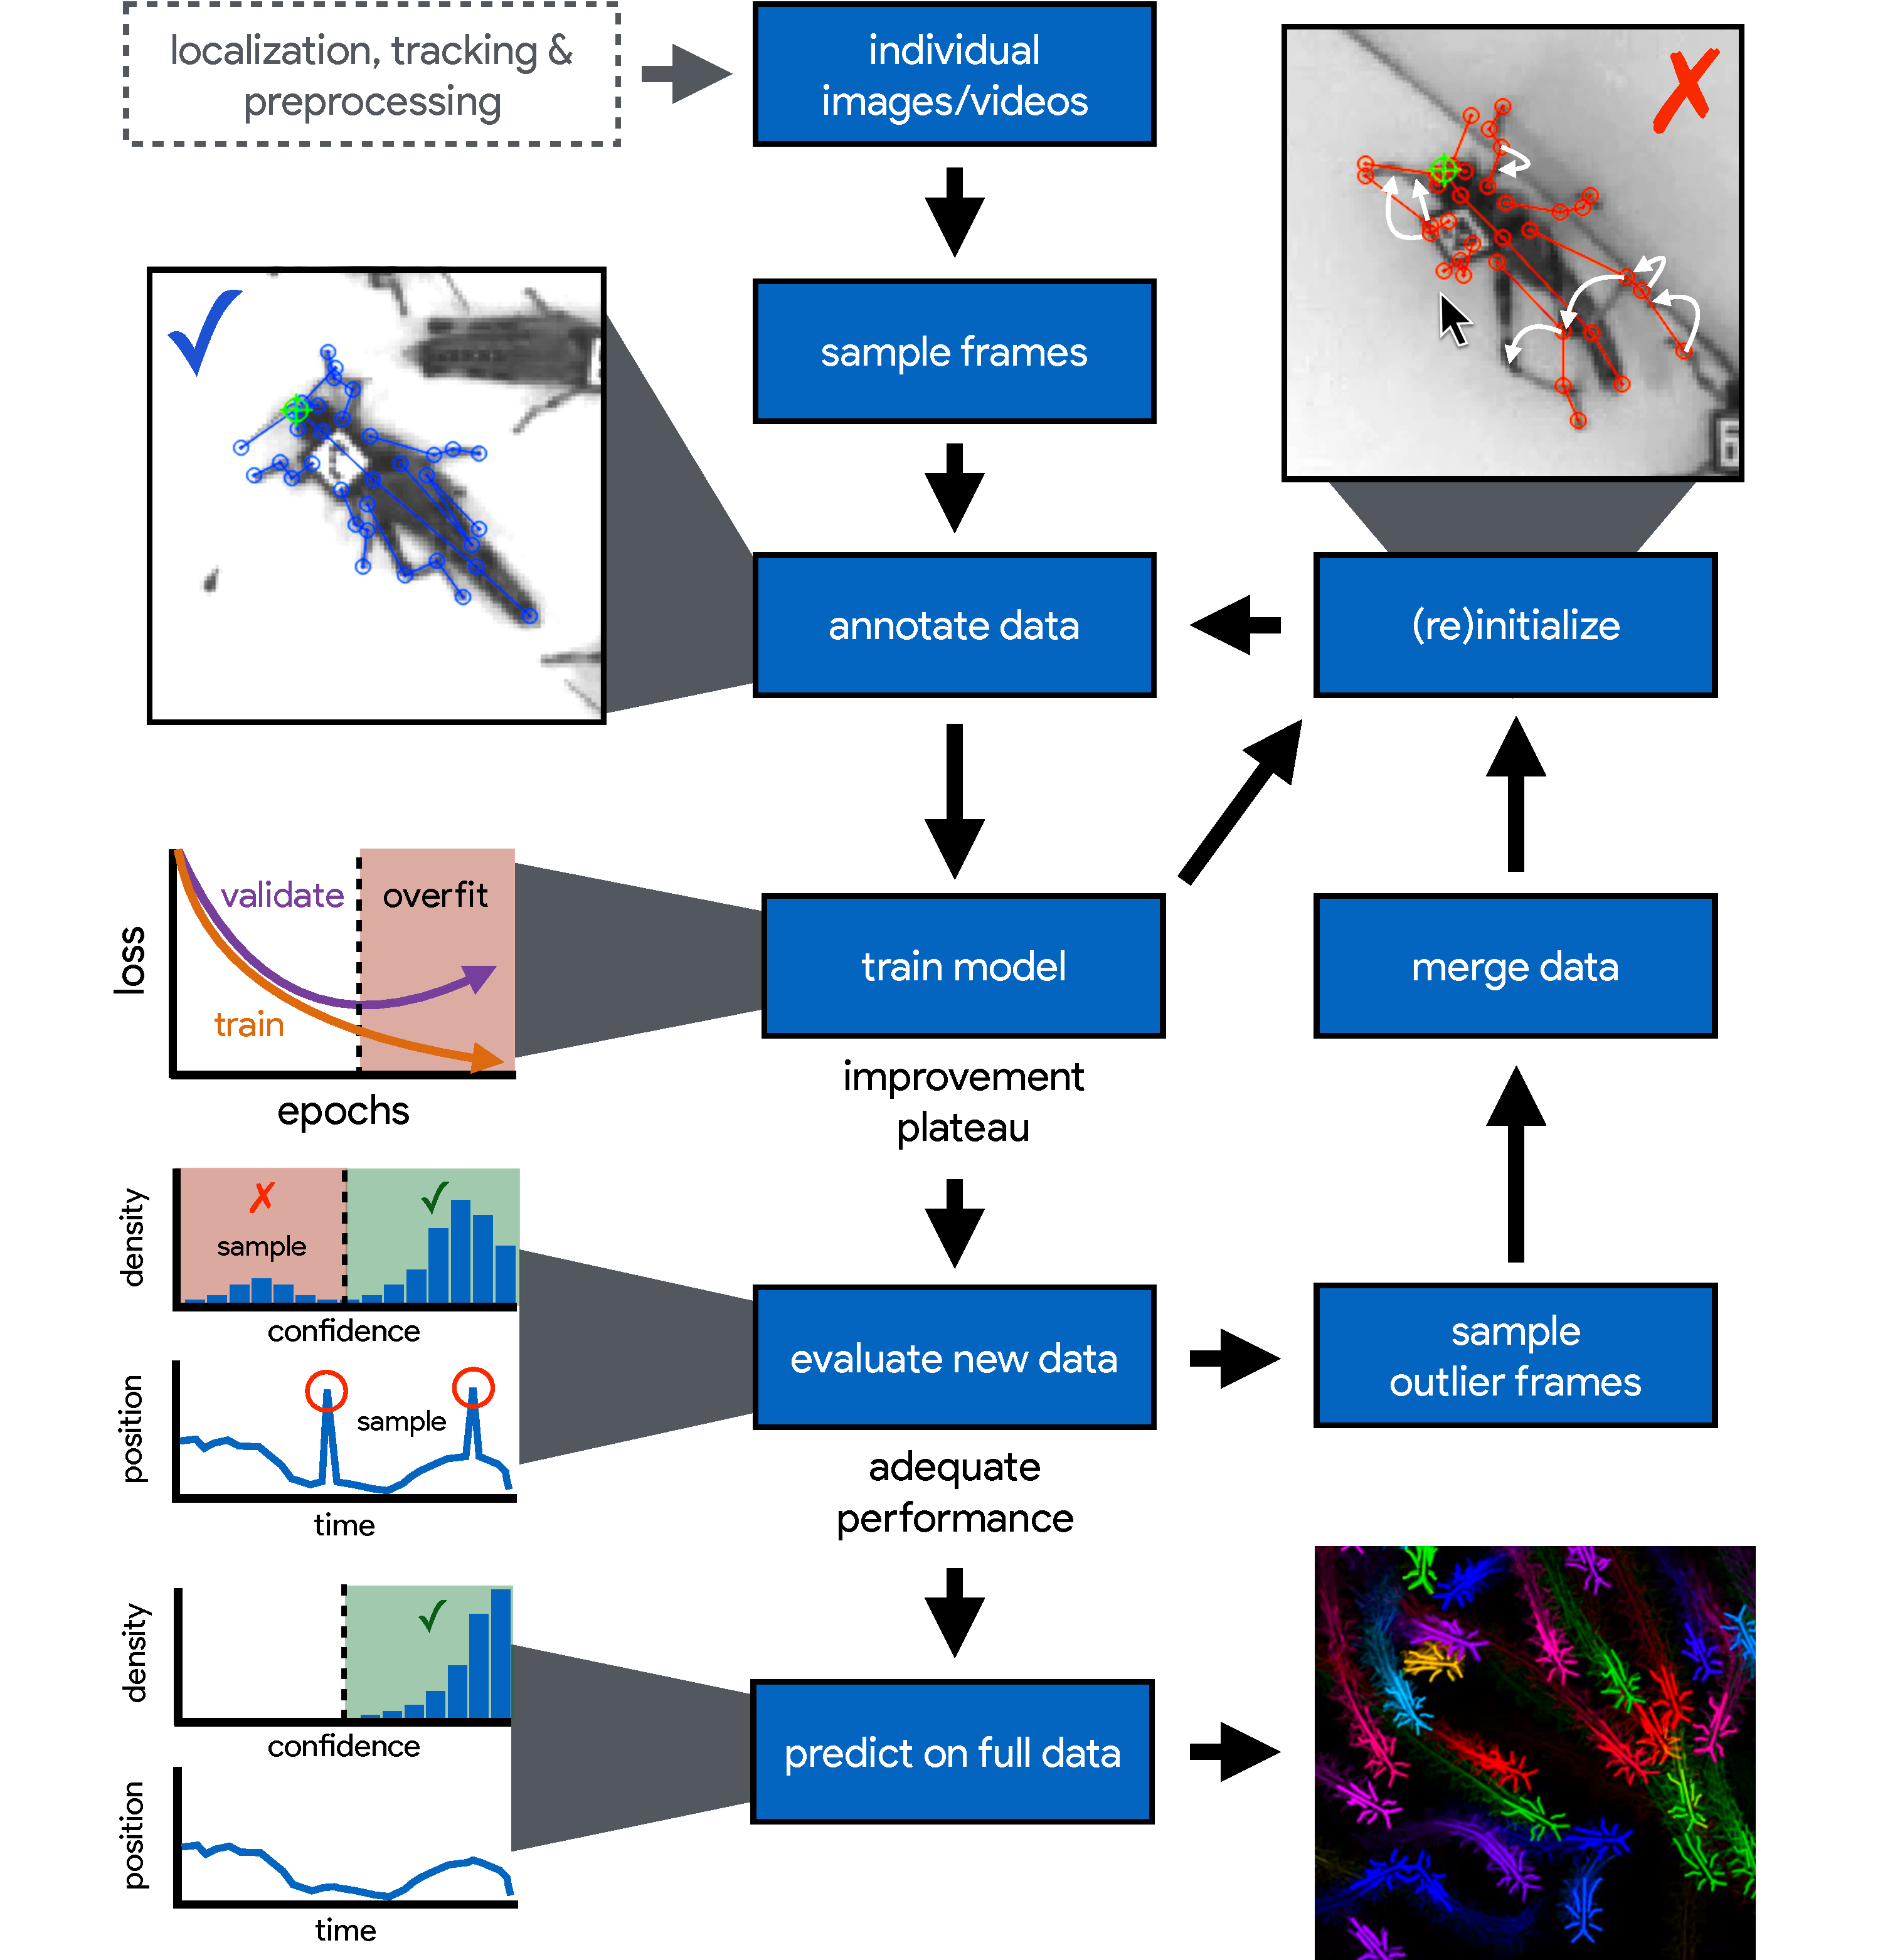
\includegraphics[width=0.95\linewidth]{Graving_IMPRS_Thesis/figures/workflow_figure.pdf}

\caption{An illustration of the workflow for DeepPoseKit. Multi-individual images are localized, tracked, and preprocessed into individual images, which is not required for single-individual image datasets. An initial image set is sampled, annotated, and then iteratively updated using the active learning approach described by \cite{pereira2019fast} (see Appendix \ref{app:training_data}). As annotations are made, the model is trained (Figure \ref{fig:model_training_figure}) with the current training set and keypoint locations are initialized for unannotated data to reduce the difficulty of further annotations. This is repeated until there is a noticeable improvement plateau for the initialized data---where the annotator is providing only minor corrections---and for the validation error when training the model (Appendix \ref{app:figures} Figure \ref{fig:training_prop}). New data from the full dataset are evaluated with the model, and the training set is merged with new examples that are sampled based on the model's predictive performance, which can be assessed with techniques described by \cite{mathis2018deeplabcut, nath2018} for identifying outlier frames and minimizing extreme prediction errors—shown here as the distribution of confidence scores predicted by the model and predicted body part positions with large temporal derivatives---indicating extreme errors. This process is repeated as necessary until performance is adequate when evaluating new data. The pose estimation model can then be used to make predictions for the full data set, and the data can be used for further analysis.}
\label{fig:workflow_figure}
\end{figure}

\begin{figure}[!htb]
    \centering
    \includegraphics{}
    \caption{A visualization of the posture data output for a group of locusts (5$\times$ speed) \url{https://youtu.be/hCa2zaoUWhs}
}
\end{figure}

\subsection{Measuring animal movement with computer vision}
Collecting high-quality behavioral data is a challenging task, and while direct observations are important for gathering qualitative data about a study system, a variety of automated methods for quantifying movement have become popular in recent years \citep{dell2014automated, anderson2014toward, kays2015terrestrial}. Methods like video monitoring and recording help to accelerate data collection and reduce the effects of human intervention, but the task of manually scoring videos is time consuming and suffers from the same limitations as direct observation, namely observer bias and mental fatigue. Additionally, due to limitations of human observers' ability to process information, many studies that rely on manual scoring use relatively small datasets to estimate experimental effects, which can lead to increased rates of statistical errors. Studies that lack the statistical resolution to robustly test hypotheses (commonly called "power" in frequentist statistics) also raise concerns about the use of animals for research, as statistical errors caused by sparse data can impact researchers' ability to accurately answer scientific questions. These limitations have led to the development of automated methods for quantifying behavior using advanced imaging technologies \citep{dell2014automated} as well as sophisticated tags and collars with GPS, accelerometry, and acoustic-recording capabilities \citep{kays2015terrestrial}. Tools for automatically measuring the behavior of individuals now play a central role in our ability to study the neurobiology and ecology of animals, and reliance on these technologies for studying animal behavior will only increase in the future.

The rapid development of computer vision hardware and software in recent years has allowed for the use of automated image-based methods for measuring behavior across many experimental contexts \citep{dell2014automated}. Early methods for quantifying movement with these techniques required highly-controlled laboratory conditions. However, because animals exhibit different behaviors depending on their surroundings \citep{strandburg2017habitat,fritz2019lowcost, akhund2019effect}, laboratory environments are often less than ideal for studying many natural behaviors. Most conventional computer vision methods are also limited in their ability to accurately track groups of individuals over time, but nearly all animals are social at some point in their life and exhibit specialized behaviors when in the presence of conspecifics \citep{strandburg2013visual, rosenthal2015revealing, jolles2017consistent,klibaite2017unsupervised,klibaite2019interacting, fritz2019lowcost, versace2019individual}. These methods also commonly track only the animal's center of mass, which reduces the behavioral output of an individual to a two-dimensional or three-dimensional particle-like trajectory. While trajectory data are useful for many experimental designs, the behavioral repertoire of an animal cannot be fully described by its aggregate locomotory output. For example, stationary behaviors, like grooming and antennae movements, or subtle differences in walking gaits cannot be reliably detected by simply tracking an animal's center of mass \citep{berman2014mapping, wiltschko2015mapping}. 

Together these factors have driven the development of software that can accurately track the positions of marked \citep{crall2015beetag, graving2017pinpoint, wild2018honeybee, boenisch2018tracking} or unmarked \citep{perez2014idtracker, romero2018idtracker} individuals as well as methods that can quantify detailed descriptions of an animal's posture over time \citep{stephens2011emergence, berman2014mapping, wiltschko2015mapping, mathis2018deeplabcut, pereira2019fast}. Recently these advancements have been further improved through the use of deep learning, a class of machine learning algorithms that learn complex statistical relationships from data \citep{lecun2015deep}. Deep learning has opened the door to accurately tracking large groups of marked \citep{wild2018honeybee, boenisch2018tracking} or unmarked \citep{romero2018idtracker} individuals and has made it possible to measure the body posture of animals in nearly any context---including in the wild \citep{nath2018}---by tracking the positions of user-defined body parts \citep{mathis2018deeplabcut, pereira2019fast}. These advances have drastically increased the quality and quantity, as well as the diversity, of behavioral data that are potentially available to researchers for answering scientific questions.

\subsection{Animal pose estimation using deep learning}
In the past, conventional methods for measuring posture with computer vision relied on species-specific algorithms \citep{uhlmann2017flylimbtracker}, highly-specialized or restrictive experimental setups \citep{mendes2013quantification, kain2013leg}, attaching intrusive physical markers to the study animal \citep{kain2013leg}, or some combination thereof. These methods also typically required expert computer-vision knowledge to use, were limited in the number or type of body parts that could be tracked \citep{mendes2013quantification}, involved capturing and handling the study animals to attach markers \citep{kain2013leg}---which is not possible for many species---and despite best efforts to minimize human involvement, often required manual intervention to correct errors \citep{uhlmann2017flylimbtracker}. All of these methods were built to work for a small range of conditions and typically required considerable effort to adapt to novel contexts.

In contrast to conventional computer-vision methods, modern deep-learning–based methods can be used to achieve near human-level accuracy in almost any scenario by manually annotating data (Figure \ref{fig:workflow_figure})—known as a \textit{training set}—and training a general-purpose image-processing algorithm—a convolutional neural network or CNN—to automatically estimate the locations of an animal's body parts directly from images (Figure \ref{fig:model_training_figure}). State-of-the-art machine learning methods, like CNNs, use these training data to parameterize a model describing the statistical relationships between a set of input data—i.e., images—and the desired output distribution—i.e., posture keypoints. After adequate training, a model can be used to make predictions on previously-unseen data from the same dataset—inputs that were not part of the training set, which is known as \textit{inference}. In other words, these models are able to generalize human-level expertise at scale after having been trained on only a relatively small number of examples. We provide more detailed background information on using CNNs for pose estimation in Appendices \ref{app:cnn}–\ref{app:overparam}.

Similar to conventional pose estimation methods, the task of implementing deep-learning models in software and training them on new data is complex and requires expert knowledge. However, in most cases, once the underlying model and training routine are implemented, a high-accuracy pose estimation model for a novel context can be built with minimal modification—often just by changing the training data. With a simplified toolkit and high-level software interface designed by an expert, even scientists with limited computer-vision knowledge can begin to apply these methods to their research. Once the barriers for implementing and training a model are sufficiently reduced, the main bottleneck for using these methods becomes collecting an adequate training set—a labor-intensive task made less time-consuming by techniques described in Appendix \ref{app:training_data}.

\cite{mathis2018deeplabcut} and \cite{pereira2019fast} were the first to popularize the use of CNNs for animal pose estimation. These researchers built on work from the human pose estimation literature (e.g., \citealt{andriluka14cvpr,insafutdinov2016deepercut,newell2016}) using a type of \textit{fully-convolutional neural network} or \textit{F-CNN} (\citealt{long2015fully}; Appendix \ref{app:fcnn}) often referred to as an \textit{encoder-decoder} model (Appendix \ref{app:fcnn} Box \ref{box:encoder_decoder_box}). These models are used to measure animal posture by training the network to transform images into probabilistic estimates of keypoint locations, known as \textit{confidence maps} (shown in Figure \ref{fig:model_training_figure}), that describe the body posture for one or more individuals. These confidence maps are processed to produce the 2-D spatial coordinates of each keypoint, which can then be used for further analysis. 

While deep-learning models typically need large amounts of training data, both \cite{mathis2018deeplabcut} and \cite{pereira2019fast} have demonstrated that near human-level accuracy can be achieved with few training examples (Appendix \ref{app:training_data}). In order to ensure generalization to large datasets, both groups of researchers introduced ideas related to iteratively refining the training set used for model fitting \citep{mathis2018deeplabcut, pereira2019fast}. In particular, \cite{pereira2019fast} describe a technique known as \textit{active learning} where a trained model is used to initialize new training data and reduce annotation time (Appendix \ref{app:training_data}). \cite{mathis2018deeplabcut} describe multiple techniques that can be used to further refine training data and minimize errors when making predictions on the full dataset. Simple methods to accomplish this include filtering data or selecting new training examples based on confidence scores or the entropy of the confidence maps from the model output. \cite{nath2018} also introduced the use temporal derivatives (i.e., speed and acceleration) and autoregressive models to identify outlier frames, which can then be labeled to refine the training set or excluded from further analysis on the final dataset (Figure \ref{fig:workflow_figure}).

\subsection{Pose estimation models and the speed-accuracy trade-off}

\cite{mathis2018deeplabcut} developed their pose estimation model, which they call \textit{DeepLabCut}, by modifying a previously-published model called \textit{DeeperCut} \citep{insafutdinov2016deepercut}. The DeepLabCut model \citep{mathis2018deeplabcut}, like the DeeperCut model, is built on the popular \textit{ResNet} architecture \citep{he2016deep}—a state-of-the-art deep-learning model used for image classification. This choice is advantageous because the use of a popular architecture allows for incorporating a pre-trained encoder to improve performance and reduce the number of required training examples \citep{mathis2018deeplabcut}, known as \textit{transfer learning} (\citealt{pratt1993discriminability}; Appendix \ref{app:training_data})---although, as will be seen, transfer learning appears to offer little improvement over a randomly-initialized model. However, this choice of of a pre-trained architecture is also disadvantageous as the model is \textit{overparameterized} with >25 million parameters. Overparameterization allows the model to make accurate predictions, but this may come with the cost of slow inference. To alleviate these effects, work from \cite{mathis2018inference} showed that inference speed for the DeepLabCut model \citep{mathis2018deeplabcut} can be improved by decreasing the resolution of input images, but this is achieved at the expense of accuracy. 

With regard to model design, \cite{pereira2019fast} implement a modified version of a model called \textit{SegNet} \citep{badrinarayanan2017segnet}, which they call \textit{LEAP} (LEAP Estimates Animal Pose), that attempts to limit model complexity and overparameterization with the goal of maximizing inference speed (see Appendix \ref{app:overparam})—however, our comparisons in this paper suggest \cite{pereira2019fast} achieved only limited success compared to the DeepLabCut model \citep{mathis2018deeplabcut}. The LEAP model is advantageous because it is explicitly designed for fast inference but has disadvantages such as a lack of robustness to data variance, like rotations or shifts in lighting, and an inability to generalize to new experimental setups. Additionally, to achieve maximum performance, the training routine for the LEAP model introduced by \cite{pereira2019fast} requires computationally expensive preprocessing that is not practical for many datasets, which makes it unsuitable for a wide range of experiments (see Appendix \ref{app:overparam} for more details).

Together the methods from \cite{mathis2018deeplabcut} and \cite{pereira2019fast} represent the two extremes of a phenomenon known as the \textit{speed-accuracy trade-off}  \citep{huang2017speed}—an active area of research in the machine learning literature. \cite{mathis2018deeplabcut} prioritize accuracy over speed by using a large overparameterized model, and \cite{pereira2019fast} prioritize speed over accuracy by using a smaller less-robust model. While this speed-accuracy trade-off can limit the capabilities of CNNs, there has been extensive work to make these models more efficient without impacting accuracy (e.g., \citealt{chollet2017xception, huang2017densely,sandler2018mobilenetv2}). To address the limitations of this trade-off, we apply recent developments from the machine learning literature and provide an effective solution to the problem.

In the case of F-CNN models used for pose estimation, improvements in efficiency and robustness have been made through the use of \textit{multi-scale inference} (Appendix \ref{app:fcnn} Box \ref{box:encoder_decoder_box}) by increasing connectivity between the model's many layers across multiple spatial scales (Appendix \ref{app:fcnn} Figure \ref{fig:stacked_densenet_figure}). Multi-scale inference implicitly allows the model to simultaneously integrate large-scale global information, such as the lighting, image background, or the orientation of the focal individual's body trunk; information from intermediate scales like anatomical geometry related to cephalization and bilateral symmetry; and fine-scale local information that could include differences in color, texture, or skin patterning for specific body parts. This multi-scale design gives the model capacity to learn the hierarchical relationships between different spatial scales and efficiently aggregate them into a joint representation when solving the posture estimation task (see Box \ref{box:encoder_decoder_box} and Appendix \ref{app:fcnn} Figure \ref{fig:stacked_densenet_figure} for further discussion)

\subsection{Individual vs. multiple pose estimation}
Most work on human pose estimation now focuses on estimating the pose of multiple individuals in an image (e.g., \citealt{cao2017realtime}). For animal pose estimation, the methods from \cite{pereira2019fast} are limited to estimating posture for single individuals—known as \textit{individual pose estimation}—while the methods from \cite{mathis2018deeplabcut} can also be extended to estimate posture for multiple individuals simultaneously---known as \textit{multiple pose estimation}. However, the majority of work on multiple pose estimation, including \cite{mathis2018deeplabcut}, has not adequately solved the tracking problem of linking individual posture data across frames in a video, especially after visual occlusions, which are common in many behavioral experiments—although recent work has attempted to address this problem \citep{iqbal2017posetrack, andriluka2018posetrack}. Additionally, as the name suggests, the task of multiple pose estimation requires exhaustively annotating images of multiple individuals—where every individual in the image must be annotated to prevent the model from learning conflicting information. This type of annotation task is even more laborious and time consuming than annotations for individual pose estimation and the amount of labor increases proportionally with the number of individuals in each frame, which makes this approach intractable for many experimental systems.

Reliably tracking the position of individuals over time is important for most behavioral studies, and there are a number of diverse methods already available for solving this problem \citep{perez2014idtracker, crall2015beetag, graving2017pinpoint, romero2018idtracker, wild2018honeybee,boenisch2018tracking}. Therefore, to avoid solving an already-solved problem of tracking individuals and to circumvent the cognitively complex task of annotating data for multiple pose estimation, the work we describe in this paper is purposefully limited to individual pose estimation---where each image contains only a single focal individual, which may be cropped from a larger multi-individual image after localization and tracking. We introduce a top-down posture estimation framework that can be readily adapted to existing behavioral analysis workflows, which could include any method for localizing and tracking individuals.

The additional step of localizing and tracking individuals naturally increases the processing time for producing posture data from raw image data, which varies depending on the algorithms being used and the number of individuals in each frame. While tracking and localization may not be practical for all experimental systems, which could make our methods difficult to apply "out-of-the-box", the increased processing time from automated tracking algorithms is a reasonable trade-off for most systems given the costly alternative of increased manual labor when annotating data. This trade-off seems especially practical when considering that the posture data produced by most multiple pose estimation algorithms still need to be linked across video frames to maintain the identity of each individual, which is effectively a bottom-up method for achieving the same result. Limiting our methods to individual pose estimation also simplifies the pose detection problem as processing confidence maps produced by the model does not require computationally-expensive local peak detection and complex methods for grouping keypoints into individual posture graphs (e.g., \citealt{insafutdinov2016deepercut, cao2017realtime}; Appendix \ref{app:fcnn}). Additionally, because individual pose estimation is such a well-studied problem in computer vision, we can readily build on state-of-the-art methods for this task (see Appendices \ref{app:fcnn} and \ref{app:sota} for details).


\section{Results}
Here we introduce fast, flexible, and robust pose estimation methods, with a software interface---a high-level programming interface (API) and graphical user-interface (GUI) for annotations---that emphasizes usability. Our methods build on the state-of-the-art for individual pose estimation (\citealt{newell2016}; Appendix \ref{app:sota}), convolutional regression models (\citealt{Jegou16}; Appendix \ref{app:fcnn} Box \ref{box:encoder_decoder_box}), and conventional computer vision algorithms \citep{guizar2008efficient} to improve model efficiency and achieve faster, more accurate results on multiple challenging pose estimation tasks. We developed two model implementations—including a new model architecture that we call \textit{Stacked DenseNet}—and a new method for processing confidence maps called \textit{subpixel maxima} that provides fast and accurate peak detection for estimating keypoint locations with subpixel precision—even at low spatial resolutions. We also discuss a modification to incorporate a hierarchical posture graph for learning the multi-scale geometry between keypoints on the animal's body, which increases accuracy when training pose estimation models. We ran experiments to optimize our approach and compared our new models to the models from \cite{mathis2018deeplabcut} (DeepLabCut) and \cite{pereira2019fast} (LEAP) in terms of speed, accuracy, training time, and generalization ability. We benchmarked these models using three image datasets recorded in the laboratory and the field—including multiple interacting individuals that were first localized and cropped from larger, multi-individual images (see "Methods" for details). 

\begin{figure}[!htb]

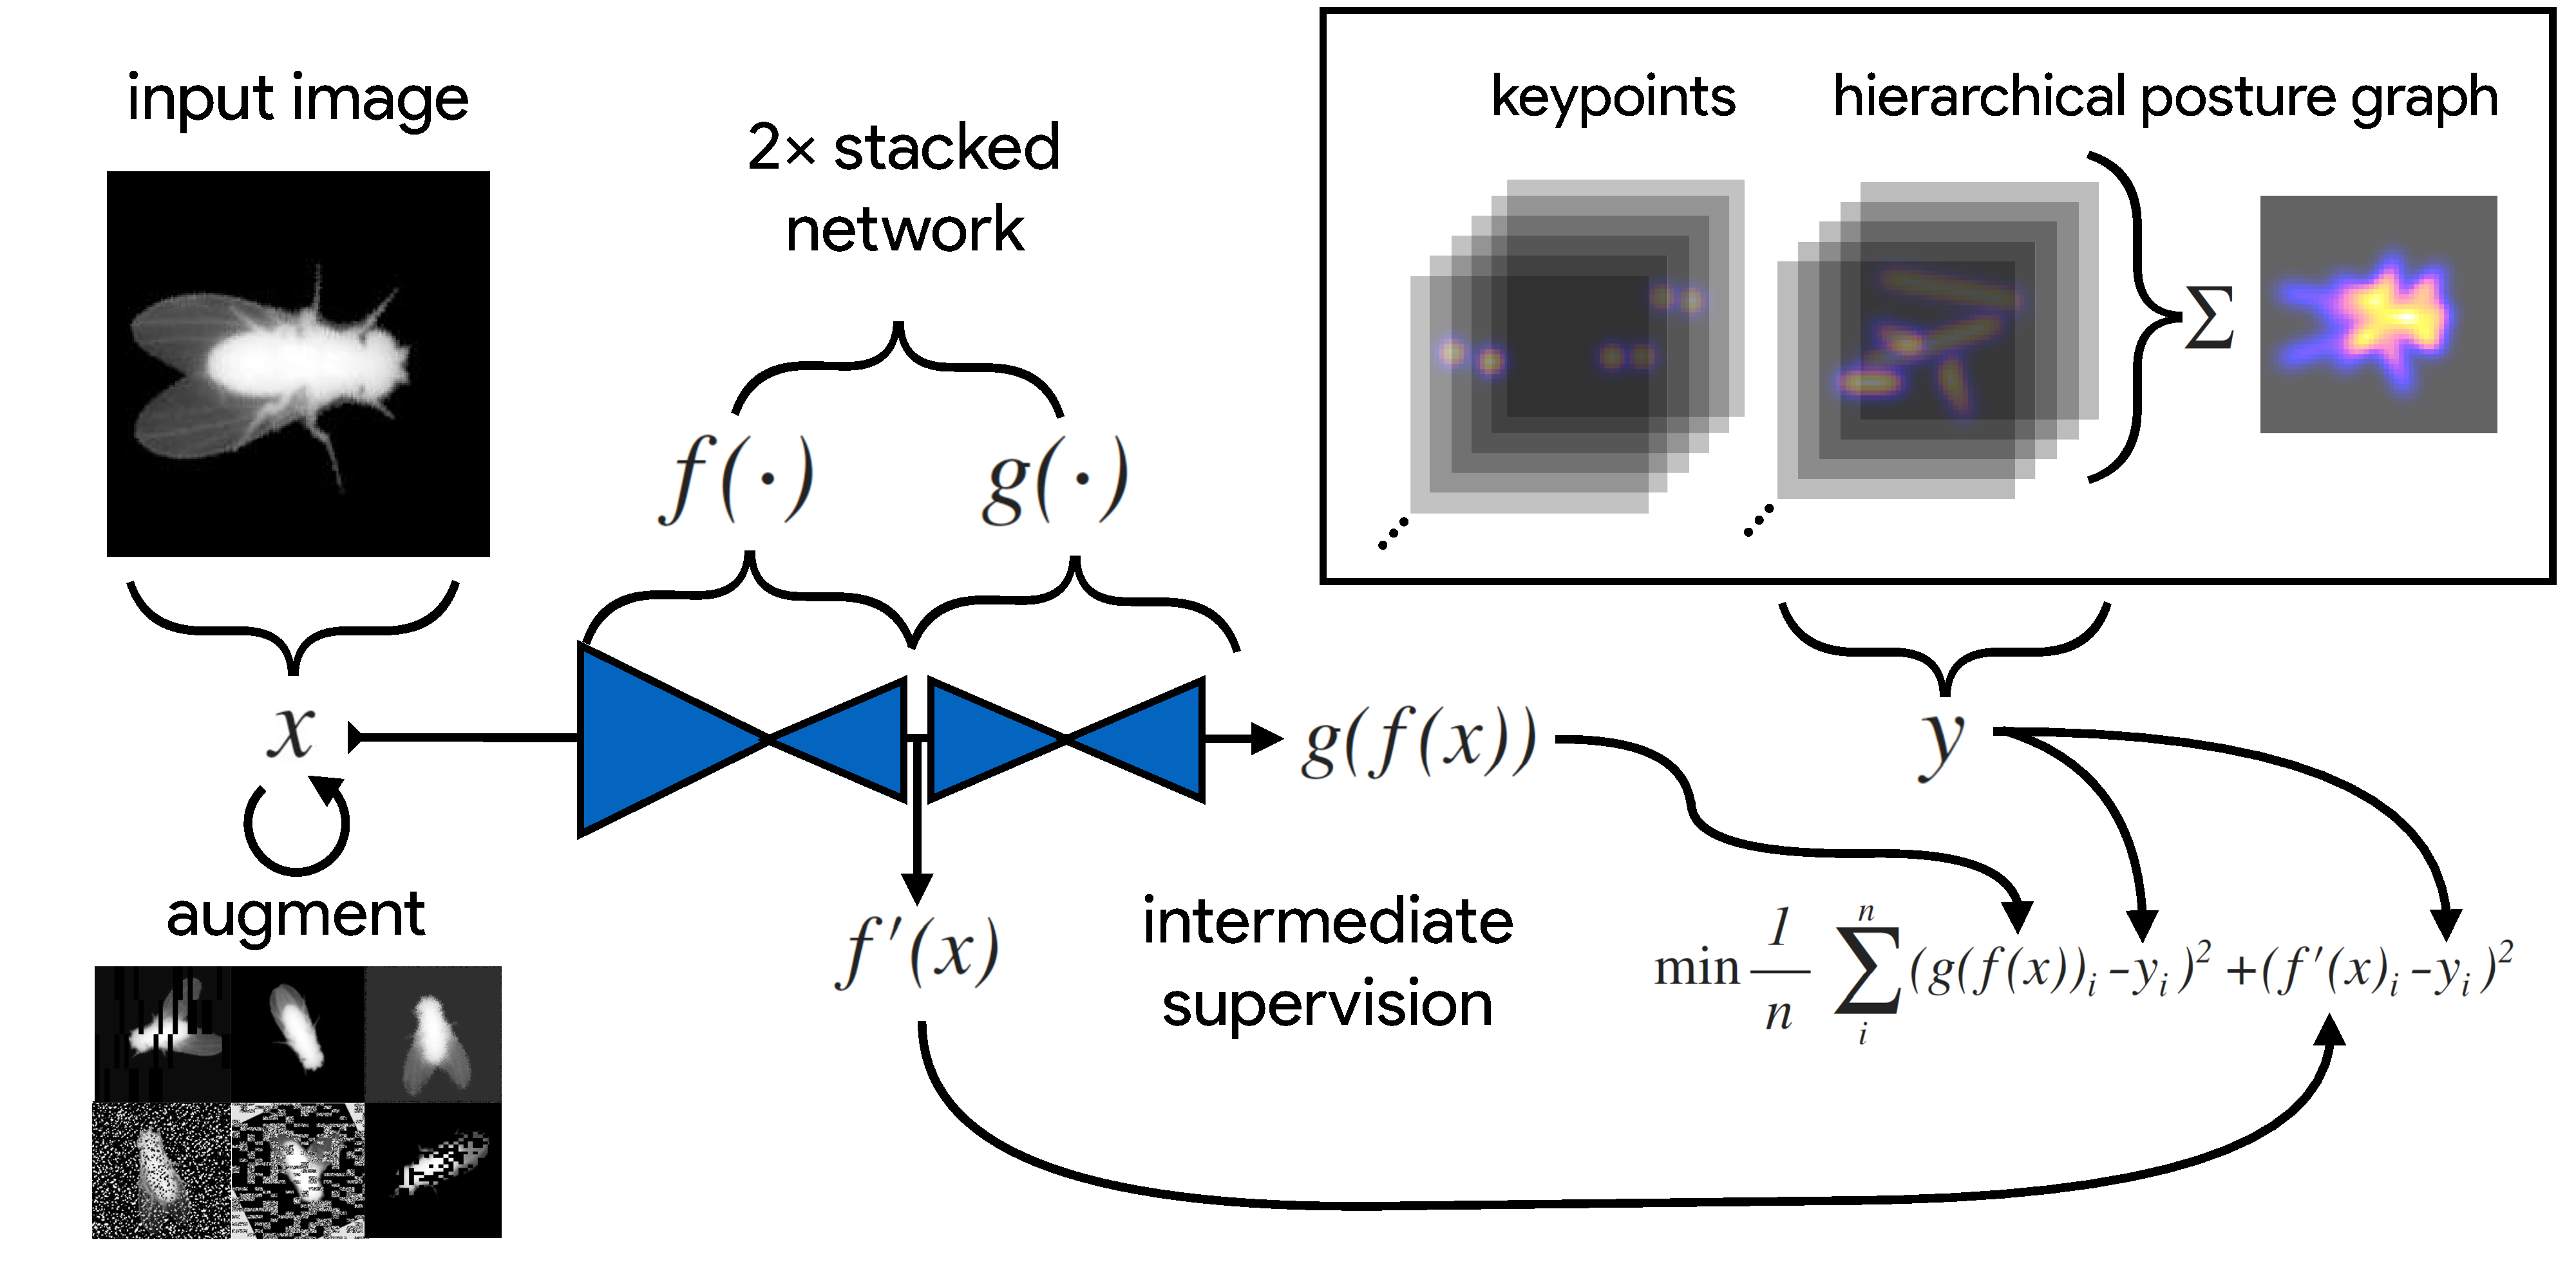
\includegraphics[width=0.95\linewidth]{Graving_IMPRS_Thesis/figures/model_training_figure.pdf}
\caption{An illustration of the model training process for our Stacked DenseNet model in DeepPoseKit (see Appendix \ref{app:cnn} for details about training models). Input images $x$ (\textbf{top-left}) are augmented (\textbf{bottom-left}) with various spatial transformations (rotation, translation, scale, etc.) followed by noise transformations (dropout, additive noise, blurring, contrast, etc.) to improve the robustness and generalization of the model. The ground truth annotations are then transformed with matching spatial augmentations (not shown for the sake of clarity) and used to draw the confidence maps $y$ for the keypoints and hierarchical posture graph (\textbf{top-right}). The images $x$ are then passed through the network to produce a multidimensional array $g(f(x))$—a stack of images corresponding to the keypoint and posture graph confidence maps for the ground truth $y$. Mean squared error between the outputs for both networks $g(f(x))$ and $f^{\prime}(x)$ and the ground truth data $y$ is then minimized (\textbf{bottom-right}), where $f^{\prime}(x)$ indicates a subset of the output from $f(x)$—only those feature maps being optimized to reproduce the confidence maps for the purpose of intermediate supervision (Appendix \ref{app:sota}). The loss function is minimized until the validation loss stops improving—indicating that the model has converged or is starting to overfit to the training data.}
\label{fig:model_training_figure}

\end{figure}


\subsection{An end-to-end pose estimation framework}
We provide a full-featured, extensible, and easy-to-use software package that is written entirely in the Python programming language (Python Software Foundation) and is built on the popular Keras deep-learning package \citep{chollet2015keras}—using TensorFlow as a backend \citep{tensorflow2015-whitepaper}. Our software is a complete, end-to-end pipeline (Figure \ref{fig:workflow_figure}) with a custom GUI for creating annotated training data with active learning similar to \citeauthor{pereira2019fast} (\citeyear{pereira2019fast}; Appendix \ref{app:training_data}), as well as a flexible pipeline for data augmentation (\citealt{jung2018imgaug}; Appendix \ref{app:training_data}; shown in Figure \ref{fig:model_training_figure}), model training and evaluation (Figure \ref{fig:model_training_figure}; Appendix \ref{app:cnn}), and running inference on new data. We designed our high-level programming interface using the same guidelines from Keras \citep{chollet2015keras} to allow the user to go from idea to result as quickly as possible, and we organized our software into a Python module called \textit{DeepPoseKit}. The code, documentation, and examples for our entire software package are freely available at \url{https://github.com/jgraving/deepposekit} under a permissive open-source license. 


\subsection{Our pose estimation models}
To achieve the goal of “fast animal pose estimation” introduced by \cite{pereira2019fast}, while maintaining the robust predictive power of models like DeepLabCut \citep{mathis2018deeplabcut}, we implemented two fast pose estimation models that extend the state-of-the-art model for individual pose estimation introduced by \cite{newell2016} and the current state-of-the art for convolutional regression from \cite{Jegou16}. Our model implementations use fewer parameters than both the DeepLabCut model \citep{mathis2018deeplabcut} and LEAP model \citep{pereira2019fast} while simultaneously removing many of the limitations of these architectures. 

In order to limit overparameterization while minimizing performance loss, we designed our models to allow for multi-scale inference (Appendix \ref{app:fcnn} Box \ref{box:encoder_decoder_box}) while optimizing our model hyperparameters for efficiency. Our first model is a novel implementation of \textit{FC-DenseNet} from \citeauthor{Jegou16} (\citeyear{Jegou16}; Appendix \ref{app:fcnn} Box \ref{box:encoder_decoder_box}) arranged in a stacked configuration similar to \citeauthor{newell2016} (\citeyear{newell2016}; Appendix \ref{app:sota}). We call this new model Stacked DenseNet, and to the best of our knowledge, this is the first implementation of this model architecture in the literature—for pose estimation or otherwise. Further details for this model are available in Appendix \ref{app:implementation}. Our second model is a modified version of the \textit{Stacked Hourglass} model from \citeauthor{newell2016} (\citeyear{newell2016}; Appendix \ref{app:sota}) with hyperparameters that allow for changing the number of filters in each convolutional block to constrain the number of parameters—rather than using 256 filters for all layers as described in \cite{newell2016}.

\subsection[Subpixel keypoint prediction on the GPU]{Subpixel keypoint prediction on the GPU allows for fast and accurate inference}
In addition to implementing our efficient pose estimation models, we developed a new method to process model outputs to allow for faster, more accurate predictions. When using a fully-convolutional posture estimation model, the confidence maps produced by the model must be converted into coordinate values for the predictions to be useful, and there are typically two choices for making this conversion. The first is to move the confidence maps out of GPU memory and post-process them on the CPU. This solution allows for easy, flexible, and accurate calculation of the coordinates with subpixel precision \citep{insafutdinov2016deepercut, mathis2018deeplabcut}. However, CPU processing is not ideal because moving large arrays of data between the GPU and CPU can be costly, and computation on the CPU is generally slower. The other option is to directly process the confidence maps on the GPU and then move the coordinate values from the GPU to the CPU. This approach usually means converting confidence maps to integer coordinates based on the row and column index of the global maximum for each confidence map \citep{pereira2019fast}. However, this means that, to achieve a precise estimation, the confidence maps should be predicted at the full resolution of the input image, or larger, which slows down inference speed.

As an alternative to these two strategies, we introduce a new GPU-based convolutional layer that we call \textit{subpixel maxima}. This layer uses the fast, efficient, image registration algorithm introduced by \cite{guizar2008efficient} to translationally align a centered two-dimensional Gaussian filter to each confidence map via Fourier-based convolution. The translational shift between the filter and each confidence map allows us to calculate the coordinates of the global maxima with high speed and subpixel precision. This technique allows for accurate predictions of keypoint locations even if the model's confidence maps are dramatically smaller than the resolution of the input image. We compared the accuracy of our subpixel maxima layer to an integer-based maxima layer using the fly dataset from \cite{pereira2019fast} (see "Methods"). We found significant accuracy improvements across every downsampling configuration (Appendix \ref{app:figures} Figure \ref{fig:downsample_inference_speed}a). Even with confidence maps at $\tfrac{1}{8}\times$ the resolution of the original image, error did not drastically increase compared to full-resolution predictions. Making predictions for confidence maps at such a downsampled resolution allows us to achieve very fast inference >1000 Hz while maintaining high accuracy (Appendix \ref{app:figures} Figure \ref{fig:downsample_inference_speed}b).

We also provide speed comparisons with the other models we tested and find that our Stacked DenseNet model with our subpixel peak detection algorithm is faster than the DeepLabCut model \citep{mathis2018deeplabcut} for both offline (batch size = 100) and real-time speeds (batch size = 1). While we find that our Stacked DenseNet model is faster than the LEAP model \citep{pereira2019fast} for offline processing (batch size = 100), the LEAP model \citep{pereira2019fast} is significantly faster for real-time processing (batch size = 1). Our Stacked Hourglass model \citep{newell2016} is about the same or slightly faster than Stacked DenseNet for offline speeds (batch size = 100), but is much slower for real-time processing (batch size = 1). Achieving fast pose estimation using CNNs typically relies on massively parallel processing on the GPU with large batches of data or requires downsampling the images to increase speed, which increases error \citep{mathis2018inference}. These factors make fast and accurate real-time inference challenging to accomplish. Our Stacked DenseNet model, with a batch size of one, can run inference at $\sim$30-110Hz—depending on the resolution of the predicted confidence maps (Appendix \ref{app:figures} Figure \ref{fig:downsample_inference_speed}b). These speeds are faster than the DeepLabCut model \citep{mathis2018deeplabcut} and could be further improved by downsampling the input image resolution or reconfiguring the model with fewer parameters. This allows our methods to be flexibly used for real-time or closed-loop behavioral experiments with prediction errors similar to current state-of-the-art methods. 


\subsection[Learning multi-scale geometry between keypoints improves accuracy]{Learning multi-scale geometry between keypoints improves accuracy and reduces extreme errors}

Minimizing extreme prediction errors is important to prevent downstream effects on any further behavioral analysis \citep{seethapathi2019movement}---especially in the case of analyses based on time-frequency transforms like those from \cite{berman2014mapping, berman2016predictability, klibaite2017unsupervised, todd2017systematic, klibaite2019interacting} and \cite{pereira2019fast} where high magnitude errors can cause inaccurate behavioral classifications. While effects of these extreme errors can be minimized using post-hoc filters and smoothing, these post-processing techniques can remove relevant high-frequency information from time-series data, so this solution is less than ideal. One way to minimize extreme errors when estimating posture is to incorporate multiple spatial scales when making predictions (e.g., \citealt{chen2017adversarial}). Our pose estimation models are implicitly capable of using information from multiple scales (see Appendix \ref{app:fcnn} Box \ref{box:encoder_decoder_box}), but there is no explicit signal that optimizes the model to take advantage of this information when making predictions.

To remedy this, we modified the model's output to predict, in addition to keypoint locations, a hierarchical graph of edges describing the multi-scale geometry between keypoints—similar to the part affinity fields described by \cite{cao2017realtime}. This was achieved by adding an extra set of confidence maps to the output where edges in the postural graph are represented by Gaussian-blurred lines the same width as the Gaussian peaks in the keypoint confidence maps. Our posture graph output then consists of four levels: (1) a set of confidence maps for the smallest limb segments in the graph (e.g., foot to ankle, knee to hip, etc.; Figure \ref{fig:model_training_figure}), (2) a set of confidence maps for individual limbs (e.g., left leg, right arm, etc.; Figure \ref{fig:posture_confidence_map_figure}), (3) a map with the entire postural graph, and (4) a fully-integrated map that incorporates the entire posture graph and confidence peaks for all of the joint locations (Figure \ref{fig:model_training_figure}). Each level of the hierarchical graph is built from lower levels in the output, which forces the model to learn correlated features across multiple scales when making predictions.

 We find that training our Stacked DenseNet model to predict a hierarchical posture graph reduces keypoint prediction error (Appendix \ref{app:figures} Figure \ref{fig:graph_error_figure}), and because the feature maps for the posture graph can be removed from the final output during inference, this effectively improves prediction accuracy for free. Both the mean and variance of the error distributions were lower when predicting the posture graph, which suggests that learning multi-scale geometry both decreases error on average and helps to reduce extreme prediction errors. The overall effect size for this decrease in error is fairly small (<1 pixel average reduction in error), but based on the results from the zebra dataset, this modification more dramatically improves performance for datasets with higher-variance images and sparse posture graphs. Predicting the posture graph may be especially useful for animals with long slender appendages such as insect legs and antennae where prediction errors are likely to occur due to occlusions and natural variation in the movement of these body parts. These results also suggest that annotating multiple keypoints to incorporate an explicit signal for multi-scale information may help improve prediction accuracy for a specific body part of interest.

\subsection{Stacked DenseNet is fast and robust}
\label{subsec:models}
We benchmarked our new model implementations against the models \citep{pereira2019fast} and \cite{mathis2018deeplabcut}. We find that our Stacked DenseNet model outperforms both the LEAP model \citep{pereira2019fast} and the DeepLabCut model \citep{mathis2018deeplabcut} in terms of speed while also achieving much higher accuracy than the LEAP model \citep{pereira2019fast} with similar accuracy to the DeepLabCut model (\citealt{mathis2018deeplabcut}; Figure \ref{fig:speed_accuracy_api}a). We found that both the Stacked Hourglass and Stacked DenseNet models outperformed the LEAP model \citep{pereira2019fast}. Notably our Stacked DenseNet model achieved approximately 2$\times$ faster inference speeds with 3$\times$ higher mean accuracy. Not only were our models’ average prediction error significantly improved, but also, importantly, the variance was lower—indicating that our models produced fewer extreme prediction errors. At $\tfrac{1}{4}\times$ resolution, our Stacked DenseNet model consistently achieved prediction accuracy nearly identical to the DeepLabCut model \citep{mathis2018deeplabcut} while running inference at nearly 2$\times$ the speed and using only $\sim$5$\%$ of the parameters—$\sim$1.5 million vs. $\sim$26 million. Detailed results of our model comparisons are shown in Figure \ref{fig:speed_accuracy_api}-Figure supplement \ref{figsupp:model_posterior_comparisons}.

While the Stacked DenseNet model used for comparisons is already fast, inference speed could be further improved by using a $\tfrac{1}{8}\times$ output without much increase in error (Appendix \ref{app:figures} Figure \ref{fig:downsample_inference_speed}) or by further adjusting the hyperparameters to constrain the size of the model. Our Stacked Hourglass implementation followed closely behind the performance of our Stacked DenseNet model and the DeepLabCut model \citep{mathis2018deeplabcut} but consistently performed more poorly than our Stacked DenseNet model in terms of prediction accuracy, so we excluded this model from further analysis. We were also able to reproduce the results reported by \cite{pereira2019fast} that the LEAP model and the Stacked Hourglass model \citep{newell2016} have similar average prediction error for the fly dataset. However, we also find that the LEAP model \citep{pereira2019fast} has much higher variance, which suggests it is more prone to extreme prediction errors—a problem for further data analysis.

\subsection{Stacked DenseNet trains quickly and requires few training examples}
To further compare models, we used our zebra dataset to assess the training time needed for our Stacked DenseNet model, the DeepLabCut model \citep{mathis2018deeplabcut}, and the LEAP model \citep{pereira2019fast} to reach convergence as well as the amount of training data needed for each model to generalize to new data from outside the training set. We find that our Stacked DenseNet model, the DeepLabCut model \citep{mathis2018deeplabcut}, and the LEAP model \citep{pereira2019fast} all fully converge in just a few hours and reach reasonably high accuracy after only an hour of training (Appendix \ref{app:figures} Figure \ref{fig:training_time}). However, it appears that our Stacked DenseNet model tends to converge to a good minimum faster than both the DeepLabCut model \citep{mathis2018deeplabcut} and the LEAP model \citep{pereira2019fast}.

We also show that our Stacked DenseNet model achieves good generalization with few training examples and without the use of transfer learning (Appendix \ref{app:figures} Figure \ref{fig:training_prop}). These results demonstrate that, when combined with data augmentation, as few as five training examples can be used as an initial training set for labelling keypoints with active learning (Figure \ref{fig:workflow_figure}). Additionally, because our analysis shows that generalization to new data plateaus after approximately 100 labeled training examples, it appears that 100 training examples is a reasonable minimum size for a training set---although the exact number will likely change depending the variance of the image data being annotated. To further examine the effect of transfer learning on model generalization, we compared performance between the DeepLabCut model \citep{mathis2018deeplabcut} initialized with weights pretrained on the ImageNet database \citep{deng2009imagenet} vs. the same model with randomly-initialized weights (Appendix \ref{app:figures} Figure \ref{fig:training_prop}). As postulated by \cite{mathis2018deeplabcut}, we find that transfer learning does provide some benefit to the DeepLabCut model's ability to generalize. However, the effect size of this improvement is small with a mean reduction in Euclidean error of <0.5 pixel. Together these results indicate that transfer learning is helpful, but not required, for deep learning models to achieve good generalization with limited training data.

\begin{figure}[!htb]

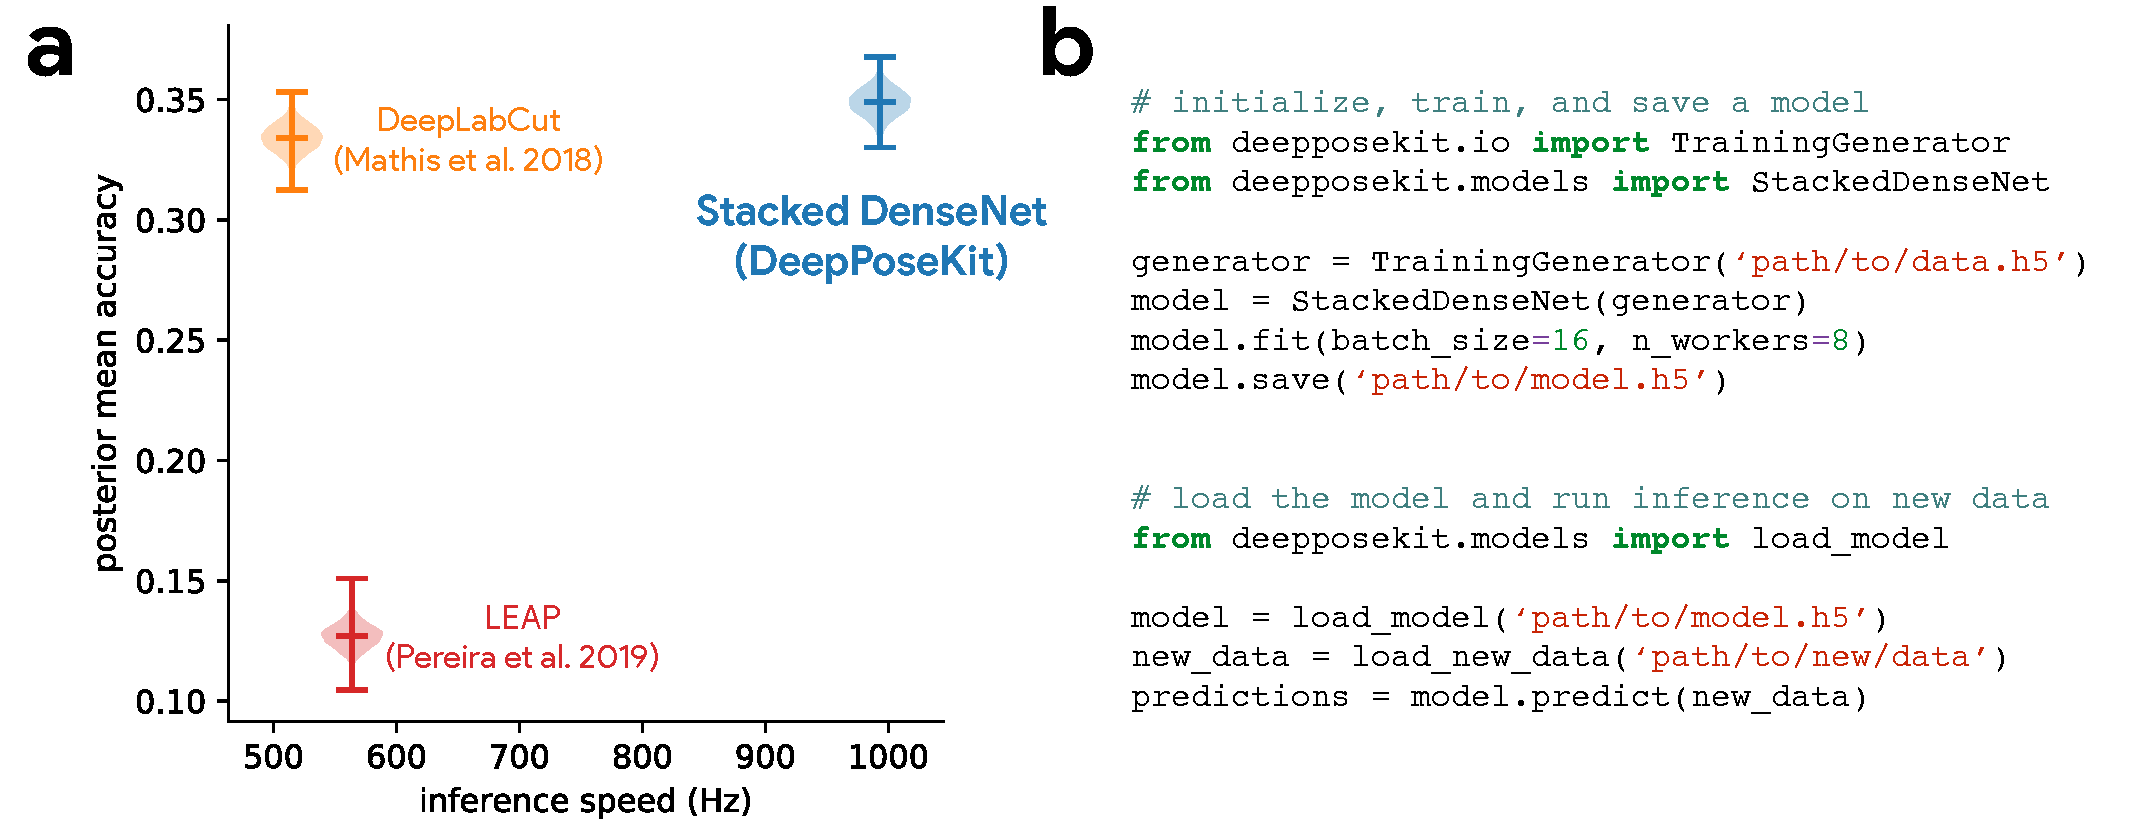
\includegraphics[width=0.95\linewidth]{Graving_IMPRS_Thesis/figures/speed_accuracy_api_figure.pdf}
\caption{Our Stacked DenseNet model estimates posture at approximately 2$\times$—or greater—the speed of the LEAP model \citep{pereira2019fast} and the DeepLabCut model \citep{mathis2018deeplabcut} while also achieving similar accuracy to the DeepLabCut model \citep{mathis2018deeplabcut}—shown here as mean accuracy $(1 + \textrm{Euclidean error})^{-1}$ for our most challenging dataset of multiple interacting Grévy's zebras (\textit{E. grevyi}) recorded in the wild (\textbf{a}). See Figure \ref{fig:speed_accuracy_api} supplement \ref{figsupp:model_posterior_comparisons} for further details. Our software interface is designed to be straightforward but flexible. We include many options for expert users to customize model training with sensible default settings to make pose estimation as easy as possible for beginners. For example, training a model and running inference on new data requires writing only a few lines of code and specifying some basic settings (\textbf{b}).}
\label{fig:speed_accuracy_api}
%\figdata{Raw prediction errors used for model comparisons in Figure \ref{fig:speed_accuracy_api}-Figure supplement \ref{figsupp:model_posterior_comparisons}. See "Methods" for details.}\label{figdata:model_comparisons}


\end{figure}
\begin{figure}[!htb]
    \centering
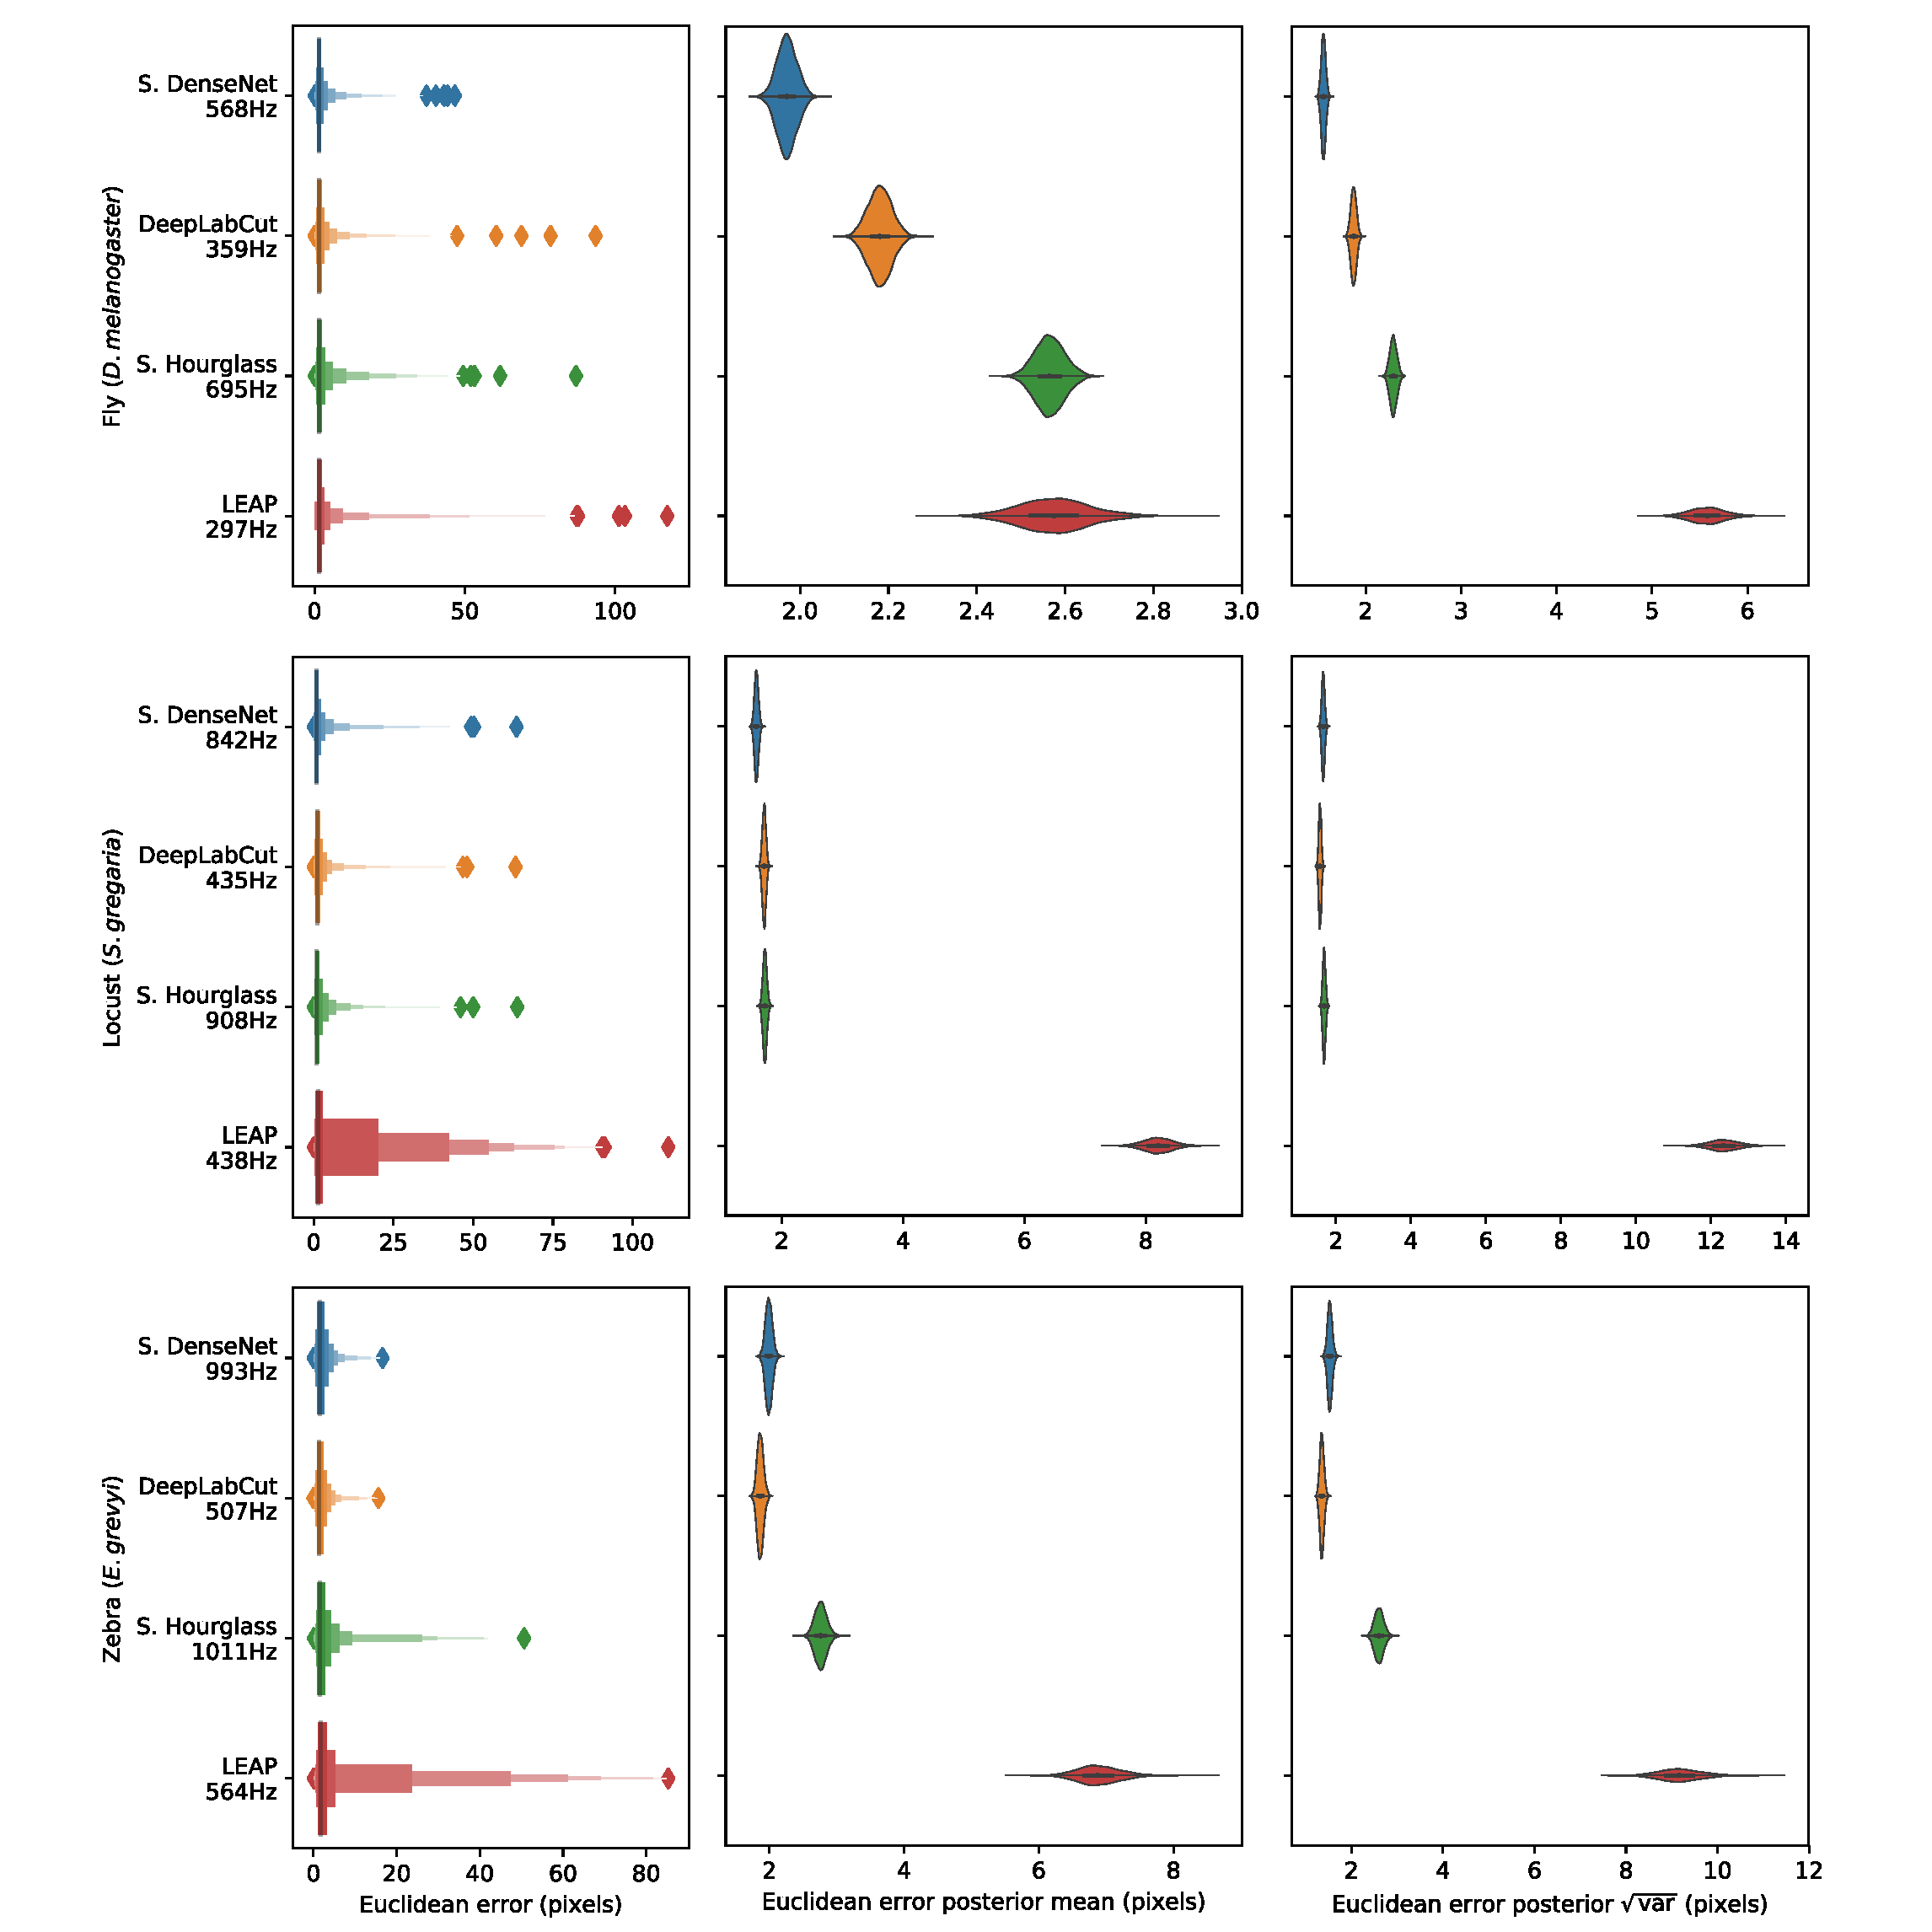
\includegraphics[width=\linewidth]{Graving_IMPRS_Thesis/figures/model_posteriors_figure.pdf}
\caption{Euclidean error distributions for each model across our three datasets. Letter-value plots (\textbf{left}) show the raw error distributions for each model. Violinplots of the posterior distributions for the mean and variance (\textbf{right}) show statistical differences between the error distributions. Overall the LEAP model \citep{pereira2019fast} was the worst performer on every dataset in terms of both mean and variance. Our Stacked Densenet model was the best performer for the fly dataset, while our Stacked DenseNet model and the DeepLabCut model \citep{mathis2018deeplabcut} both performed equally well on the locust and zebra datasets. The posteriors for the DeepLabCut model \citep{mathis2018deeplabcut} and our Stacked DenseNet model are highly overlapping for these datasets, which suggests they are not statistically discernible from one another. Our Stacked Hourglass model \citep{newell2016} performed equally to the DeepLabCut model \citep{mathis2018deeplabcut} and our Stacked DenseNet model for the locust dataset but performed slightly worse for the fly and zebra datasets.}
\label{figsupp:model_posterior_comparisons}
\end{figure}


\section{Discussion}
Here we have presented a new software toolkit, called DeepPoseKit, for estimating animal posture using deep learning models. We built on the state-of-the-art for individual pose estimation using convolutional neural networks to achieve fast inference without reducing accuracy or generalization ability. Our new pose estimation model, called Stacked DenseNet, offers considerable improvements (Figure \ref{fig:speed_accuracy_api}a; Figure supplement \ref{figsupp:model_posterior_comparisons}) over the models from \cite{mathis2018deeplabcut} (DeepLabCut) and \cite{pereira2019fast} (LEAP), and our software framework also provides a simplified interface (Figure \ref{fig:speed_accuracy_api}b) for using these advanced tools to measure animal behavior and locomotion. We tested our methods across a range of datasets from controlled laboratory environments with single individuals to challenging field situations with multiple interacting individuals and variable lighting conditions. We found that our methods perform well for all of these situations and require few training examples to achieve good predictive performance on new data---without the use of transfer learning. We ran experiments to optimize our approach and discovered that some straightforward modifications can greatly improve speed and accuracy. Additionally, we demonstrated that these modifications improve not the just the average error but also help to reduce extreme prediction errors—a key determinant for the reliability of subsequent statistical analysis.

While our results offer a good-faith comparison of the available methods for animal pose estimation, there is inherent uncertainty that we have attempted to account for but may still bias our conclusions. For example, deep learning models are trained using stochastic optimization algorithms that give different results with each replicate, and the Bayesian statistical methods we use for comparison are explicitly probabilistic in nature. There is also great variability across hardware and software configurations when using these models in practice \citep{mathis2018inference}, so performance may change across experimental setups and datasets. Additionally, we demonstrated that some models may perform better than others for specific applications (Figure \ref{fig:speed_accuracy_api} supplement \ref{figsupp:model_posterior_comparisons}), and to account for this, our toolkit offers researchers the ability to choose the model that best suits their requirements—including the LEAP model \citep{pereira2019fast} and the DeepLabCut model \citep{mathis2018deeplabcut}.  

We highlighted important considerations when using CNNs for pose estimation and reviewed the progress of fully-convolutional regression models from the literature. The latest advancements for these models have been driven mostly by a strategy of adding more connections between layers to increase performance and efficiency (e.g., \citealt{Jegou16}). Future progress for this class of models may require better loss functions \citep{goodfellow2014generative, johnson2016perceptual, chen2017adversarial, zhang2018unreasonable} that more explicitly model the spatial dependencies within a scene, models that incorporate the temporal structure of the data \citep{seethapathi2019movement}, and more mathematically-principled approaches (e.g., \citealt{weigert2018content, roy2018bayesian}) such as the application of formal probabilistic concepts \citep{kendall2017uncertainties} and Bayesian inference at scale \citep{tran2018simple}. 

Measuring behavior is a critical factor for many studies in neuroscience \citep{krakauer2017neuroscience}. Understanding the connections between brain activity and behavioral output requires detailed and objective descriptions of body posture that match the richness and resolution neural measurement technologies have provided for years \citep{anderson2014toward,berman2018measuring,brown2018ethology}, which our methods and other deep-learning–based tools provide \citep{mathis2018deeplabcut, pereira2019fast}. We have also demonstrated the possibility that our toolkit could be used for real-time inference, which allows for closed-loop experiments where sensory stimuli or optogenetic stimulation are controlled in response to behavioral measurements (e.g., \citealt{bath2014flymad,stowers2017virtual}). Using real-time measurements in conjunction with optogenetics or thermogenetics may be key to disentangling the causal structure of motor output from the brain—especially given that recent work has shown an animal's response to optogenetic stimulation can differ depending on the behavior it is currently performing \citep{cande2018optogenetic}. Real-time behavioral quantification is also particularly important as closed-loop virtual reality is quickly becoming an indispensable tool for studying sensorimotor relationships in individuals and collectives \citep{stowers2017virtual}. 

Quantifying individual movement is essential for revealing the genetic \citep{kain2012phototactic, brown2013dictionary, ayroles2015behavioral} and environmental \citep{bierbach2017behavioural, akhund2019effect, versace2019individual} underpinnings of phenotypic variation in behavior—as well as the phylogeny of behavior (e.g., \citealt{berman2014mappingv1}). Measuring individual behavioral phenotypes requires tools that are robust, scaleable, and easy-to-use, and our approach offers the ability to quickly and accurately quantify the behavior of many individuals in great detail. When combined with tools for genetic manipulations \citep{ran2013genome,doudna2014new}, high-throughput behavioral experiments \citep{alisch2018maple, javer2018open, werkhoven2019margo}, and behavioral analysis (e.g., \citealt{berman2014mapping, wiltschko2015mapping}), our methods could help to provide the data resolution and statistical power needed for dissecting the complex relationships between genes, environment, and behavioral variation.

When used together with other tools for localization and tracking (e.g., \citealt{perez2014idtracker, crall2015beetag, graving2017pinpoint, romero2018idtracker, wild2018honeybee,boenisch2018tracking}), our methods are capable of reliably measuring posture for multiple interacting individuals. The importance of measuring detailed representations of individual behavior when studying animal collectives has been well established \citep{strandburg2013visual,rosenthal2015revealing,strandburg2015shared,strandburg2017habitat}. Estimating body posture is an essential first step for unraveling the sensory networks that drive group coordination, such as vision-based networks measured via raycasting \citep{strandburg2013visual,rosenthal2015revealing}. Additionally, using body pose estimation in combination with computational models of behavior (e.g., \citealt{Costa1501}, \citealt{wiltschko2015mapping}) and unsupervised behavioral classification methods (e.g., \citealt{berman2014mapping}, \citealt{pereira2019fast}) may allow for further dissection of how information flows through groups by revealing the networks of behavioral contagion across multiple timescales and sensory modalities. While we have provided a straightforward solution for applying existing pose estimation methods to measure collective behavior, there still remain many challenging scenarios where these methods would fail. For example, tracking posture in a densely-packed bee hive or school of fish would require novel solutions to deal with the 3-D nature of individual movement, which includes maintaining individual identities and dealing with the resulting occlusions that go along with imaging these types of biological systems.  

When combined with unmanned aerial vehicles (UAVs; \citealt{schiffman2014drones}) or other field-based imaging \citep{fritz2019lowcost}, applying these methods to the study of individuals and groups in the wild can provide high-resolution behavioral data that goes beyond the capabilities of current GPS and accelerometry-based technologies \citep{nagy2010hierarchical,nagy2013context,kays2015terrestrial,strandburg2015shared,strandburg2017habitat,flack2018local}—especially for species that are impractical to study with tags or collars. Additionally, by applying these methods in conjunction with 3-D habitat reconstruction—using techniques from photogrammetry  \citep{strandburg2017habitat, fritz2019lowcost}—field-based studies can begin to integrate fine-scale behavioral measurements with the full 3-D environment in which the behavior evolved. Future advances will likely allow for the calibration and synchronizaton of imaging devices across multiple UAVs (e.g. \citealt{price2018deep, Nitin_ICCV_19}). This would make it possible to measure the full 3-D posture of wild animals (e.g. \citealt{Zuffi:ICCV:2019}) in scenarios where fixed camera systems (e.g. \citealt{nath2018}) would not be tractable, such as during migratory or predation events. When combined, these technologies could allow researchers to address questions about the behavioral ecology of animals that were previously impossible to answer.

Computer vision algorithms for measuring behavior at the scale of posture have rapidly advanced in a very short time; nevertheless, the task of pose estimation is far from solved. There are hard limitations to this current generation of pose estimation methods that are primarily related to the requirement for human annotations and user-defined keypoints---both in terms of the number of keypoints, the specific body parts being tracked, and the inherent difficulty of incorporating temporal information into the annotation and training procedure. Often the body parts chosen for annotation are an obvious fit for the experimental design and have reliably-visible reference points on the animal's body that make them easy to annotate. However, in many cases the required number and type of body parts needed for data analysis may not so obvious---such as in the case of unsupervised behavior classification methods \citep{berman2014mapping, pereira2019fast}. Additionally, the reference points for labeling images with keypoints can be hard to define and consistently annotate across images, which is often the case for soft or flexible-bodied animals like worms and fish. Moreover, due to the laborious nature of annotating keypoints, the current generation of methods also rarely takes into account the natural temporal structure of the data, instead treating each video frame as a statistically independent event, which can lead to extreme prediction errors (reviewed by \citealt{seethapathi2019movement}). Extending these methods to track the full three-dimensional posture of animals also typically requires the use of multiple synchronized cameras \citep{nath2018, gunel2019deepfly3d}, which increases the cost and complexity of creating an experimental setup, as well as the manual labor required for annotating a training set, which must include labeled data from every camera view.

These limitations make it clear that fundamentally-different methods may be required to move the field forward. Future pose estimation methods will likely replace human annotations with fully-articulated volumetric 3-D models of the animal's body (e.g., \citealt{zuffi20173d, Zuffi:ICCV:2019}), and the 3-D scene will be learned in an unsupervised or weakly-supervised way (e.g., \citealt{jaques2019physics, Zuffi:ICCV:2019}), where the shape, position, and posture of the animal's body, the camera position and lens parameters, and the background environment and lighting conditions will all be jointly learned directly from 2-D images by a deep-learning model \citep{ TensorflowGraphicsIO2019, Zuffi:ICCV:2019}. These \textit{inverse graphics models} \citep{kulkarni2015deep, sabour2017dynamic, TensorflowGraphicsIO2019} will likely take advantage of recently-developed differentiable graphics engines that allow 3-D rendering parameters to be straightforwardly controlled using computationally-efficient optimization methods \citep{Zuffi:ICCV:2019, TensorflowGraphicsIO2019}. After optimization, the volumetric 3-D timeseries data predicted by the deep learning model could be used directly for behavioral analysis or specific keypoints or body parts could be selected for analysis post-hoc. In order to more explicitly incorporate the natural statistical properties of the data, these models will also likely rely on the use of perceptual \citep{johnson2016perceptual, zhang2018unreasonable, Zuffi:ICCV:2019} and adversarial \citep{goodfellow2014generative, chen2017adversarial, kanazawa2019learning} loss functions that incorporate spatial dependencies within the scene rather than modelling each video frame as a set of statistically independent pixel distributions---as is the case with current methods that use factorized likelihood functions such as pixel-wise mean squared error (e.g., \citealt{pereira2019fast}) or cross-entropy loss (e.g., \citealt{mathis2018deeplabcut}). Because there would be limited or no requirement for human-provided labels, these models could also be easily modified to incorporate the temporal structure of the data using autoregressive representations (e.g., \citealt{van2016conditional, oord2016wavenet, kanazawa2019learning, kumar2019videoflow}), rather than modeling the scene in each video frame as a statistically independent event. Together these advances could lead to larger, higher-resolution, more reliable behavioral datasets that could revolutionize our understanding of relationships between behavior, the brain, and the environment.


In conclusion, we have presented a new toolkit, called DeepPoseKit, for automatically measuring animal posture from images. We combined recent advances from the literature to create methods that are fast, robust, and widely applicable to a range of species and experimental conditions. When designing our framework we emphasized usability across the entire software interface, which we expect will help to make these advanced tools accessible to a wider range of researchers. The fast inference and real-time capabilities of our methods should also help further reduce barriers to previously intractable questions across many scientific disciplines—including neuroscience, ethology, and behavioral ecology—both in the laboratory and the field.


\section{Methods}

We ran three main experiments to test and optimize our approach. First, we compared our new subpixel maxima layer to an integer-based global maxima with downsampled outputs ranging from 1$\times$ to $\tfrac{1}{16}\times$ the input resolution using our Stacked DenseNet model. Next, we tested if training our Stacked DenseNet model to predict the multi-scale geometry of the posture graph improves accuracy. Finally, we compared our model implementations of Stacked Hourglass and Stacked DenseNet to the models from \cite{pereira2019fast} (LEAP) and \cite{mathis2018deeplabcut} (DeepLabCut), which we also implemented in our framework (see Appendix \ref{app:implementation} for details). We assessed both the inference speed and prediction accuracy of each model as well as training time and generalization ability. When comparing these models we incorporated the relevant improvements from our experiments—including subpixel maxima and predicting multi-scale geometry between keypoints—unless otherwise noted (see Appendix \ref{app:implementation}).

While we do make comparisons to the DeepLabCut model \citep{mathis2018deeplabcut} we do not use the same training routine as \cite{mathis2018deeplabcut} and \cite{nath2018}, who use binary cross-entropy loss for optimizing the confidence maps in addition to the location refinement maps described by \cite{insafutdinov2016deepercut}. We made this modification in order to hold the training routine constant for each model while only varying the model itself. However, we find that these differences between training routines effectively have no impact on performance when the models are trained using the same dataset and data augmentations (Appendix \ref{app:implementation} Figure \ref{fig:dlc_comparison}). We also provide qualitative comparisons to demonstrate that, when trained with our DeepPoseKit framework, our implementation of the DeepLabCut model \citep{mathis2018deeplabcut} appears to produce fewer prediction errors than the original implementation from \cite{mathis2018deeplabcut, nath2018} when applied to a novel video (Appendix \ref{app:implementation} Figure \ref{fig:dlc_comparison}-Figure supplements \ref{figsupp:dlc_tsplot} and \ref{figsupp:dlc_dxtsplot}; Appendix \ref{app:implementation} Figure \ref{fig:dlc_comparison}-video \ref{videosupp:dlcsv1}). 


\subsection{Datasets}
We performed experiments using the vinegar or "fruit" fly (\textit{Drosophila melanogaster}) dataset (Figure \ref{fig:posture_confidence_map_figure}-video \ref{videosupp:sv1}) provided by \cite{pereira2019fast}, and to demonstrate the versatility of our methods we also compared model performance across two previously unpublished posture data sets from groups of desert locusts (\textit{Schistocerca gregaria}) recorded in a laboratory setting (Figure \ref{fig:posture_confidence_map_figure}-video \ref{videosupp:sv2}), and herds of Grévy's zebras (\textit{Equus grevyi}) recorded in the wild (Figure \ref{fig:posture_confidence_map_figure}-video \ref{videosupp:sv3}). The locust and zebra datasets are particularly challenging for pose estimation as they feature multiple interacting individuals—with focal individuals centered in the frame—and the latter with highly-variable environments and lighting conditions. These datasets are freely-available from \url{https://github.com/jgraving/deepposekit-data} \citep{graving2019data}.

Our locust dataset consisted of a group of 100 locusts in a circular plastic arena 1-m in diameter. The locust group was recorded from above using a high-resolution camera (Basler ace acA2040-90umNIR) and video recording system (Motif, loopbio GmbH). Locusts were localized and tracked using 2-D barcode markers \citep{graving2017pinpoint} attached to the thorax with cyanoacrylate glue, and any missing localizations ($<0.02 \%$ of the total dataset) between successful barcode reads were interpolated with linear interpolation.  Our zebra dataset consisted of variably sized groups in the wild recorded from above using a commercially-available quadcopter drone (DJI Phantom 4 Pro). Individual zebra were localized using custom deep-learning software based on Faster R-CNN \citep{ren2015faster} for predicting bounding boxes. The positions of each zebra were then tracked across frames using a linear assignment algorithm \citep{munkres1957algorithms} and data were manually verified for accuracy.

After positional tracking, the videos were then cropped using the egocentric coordinates of each individual and saved as separate videos---one for each individual. The images used for each training set were randomly selected using the k-means sampling procedure (with k=10) described by \cite{pereira2019fast} (Appendix \ref{app:training_data}) to reduce correlation between sampled images. After annotating the images with keypoints, we rotationally and translationally aligned the images and keypoints using the central body axis of the animal in each labeled image. This step allowed us to more easily perform data augmentations (see "Model training") that allow the model to make accurate predictions regardless of the animal's body size and orientation (see Appendix \ref{app:overparam}). However, this preprocessing step is not a strict requirement for training, and there is no requirement for this preprocessing step when making predictions on new unlabeled data, such as with the methods described by \cite{pereira2019fast} (Appendix \ref{app:overparam}). Before training each model we split each annotated dataset into randomly selected training and validation sets with 90\% training examples and 10\% validation examples, unless otherwise noted. The details for each dataset are described in Table \ref{tab:datasets}.

\begin{figure}[!htb]

\begin{center}
\includegraphics[width=0.9\linewidth]{Graving_IMPRS_Thesis/figures/posture_confidence_map_figure.pdf}
\end{center}
\caption{A visualization of the datasets we used to evaluate our methods (Table \ref{tab:datasets}). For each dataset, confidence maps for the keypoints (bottom-left) and posture graph (top-right) are illustrated using different colors for each map. These outputs are from our Stacked DenseNet model at $\frac{1}{4}\times$ resolution.}
\label{fig:posture_confidence_map_figure}


\end{figure}
\begin{figure}[!htb]
    \centering
    \caption{A video of a behaving fly from \cite{pereira2019fast} with pose estimation outputs visualized \url{https://youtu.be/lsnex6k4NRs}}
    \label{videosupp:sv1}
\end{figure}

\begin{figure}[!htb]
    \centering
    \caption{A video of a behaving locust with pose estimation outputs visualized. \url{https://youtu.be/b0DyyLP_Czk}}
    \label{videosupp:sv2}
\end{figure}

\begin{figure}[!htb]
    \centering
    \caption{A video of a behaving Grévy's zebra with pose estimation outputs visualized. \url{https://youtu.be/dSjaphoGHAY}}
    \label{videosupp:sv3}
\end{figure}


\begin{table}[!htb]

\caption{\label{tab:datasets}Datasets used for model comparisons.}
% Use "S" column identifier to align on decimal point 
\setlength{\tabcolsep}{2pt}
\centering
\begin{tabular}{|m{0.14\textwidth}|m{0.14\textwidth}|m{0.14\textwidth}|m{0.14\textwidth}|m{0.14\textwidth}|m{0.14\textwidth}|m{0.14\textwidth}|}
\hline
{Name} & Species   & {Resolution}  & {$\#$ Images}  & {$\#$ Keypoints} & {Individuals} & Source    \\ \hline
Vinegar fly  & \textit{Drosophila melanogaster} & {192$\times$192} & 1500 & 32 & Single & \cite{pereira2019fast} \\ \hline
Desert locust     & \textit{Schistocerca gregaria}       & 160$\times$160           & 800    & 35 & Multiple  & This paper\\ \hline
Grévy's zebra      & \textit{Equus grevyi}      & 160$\times$160              & 900    & 9 & Multiple & This paper \\ \hline
\end{tabular}

\end{table}

\subsection{Model training}
For each experiment, we set our model hyperparameters to the same configuration for our Stacked DenseNet and Stacked Hourglass models. Both models were trained with $\tfrac{1}{4}\times$ resolution outputs and a stack of two networks with two outputs where loss was applied (see Figure \ref{fig:model_training_figure}). Although our model hyperparameters could be infinitely adjusted to trade off between speed and accuracy, we compared only one configuration for each of our model implementations. These results are not meant to be an exhaustive search of model configurations as the best configuration will depend on the application. The details of the hyperparameters we used for each model are described in Appendix \ref{app:implementation}.

To make our posture estimation tasks closer to realistic conditions, incorporate prior information (Appendix \ref{app:training_data}), and properly demonstrate the robustness of our methods to rotation, translation, scale, and noise, we applied various augmentations to each data set during training (Figure \ref{fig:model_training_figure}). All models were trained using data augmentations that included random flipping, or mirroring, along both the horizontal and vertical image axes with each axis being independently flipped by drawing from a Bernoulli distribution (with $p=0.5$); random rotations around the center of the image drawn from a uniform distribution in the range [-180$\degree$, +180$\degree$); random scaling drawn from a uniform distribution in the range [90\%, 110\%] for flies and locusts and [75\%, 125\%] for zebras (to account for greater size variation in the data set); and random translations along the horizontal and vertical axis independently drawn from a uniform distribution with the range [-5\%, +5\%]---where percentages are relative to the original image size. After performing these spatial augmentations we also applied a variety of noise augmentations that included additive noise---i.e., adding or subtracting randomly-selected values to pixels; dropout---i.e., setting individual pixels or groups of pixels to a randomly-selected value; blurring or sharpening---i.e., changing the composition of spatial frequencies; and contrast ratio augmentations---i.e, changing the ratio between the highest pixel value and lowest pixel value in the image. These augmentations help to further ensure robustness to shifts in lighting, noise, and occlusions. See Appendix \ref{app:training_data} for further discussion on data augmentation.

We trained our models (Figure \ref{fig:model_training_figure}) using mean squared error loss optimized using the ADAM optimizer \citep{kingma2014adam} with a learning rate of $1\times10^{-3}$ and a batch size of 16. We lowered the learning rate by a factor of 5 each time the validation loss did not improve by more than $1\times10^{-3}$ for 10 epochs. We considered models to be converged when the validation loss stopped improving for 50 epochs, and we calculated validation error as the Euclidean distance between predicted and ground-truth image coordinates for only the best performing version of the model, which we evaluated at the end of each epoch during optimization. We performed this procedure five times for each experiment and randomly selected a new validation set for each replicate.

\subsection{Model evaluation}
Machine learning models are typically evaluated for their ability to generalize to new data, known as \textit{predictive performance}, using a held-out \textit{test set}—a subsample of annotated data that is not used for training or validation. However, due to the small size of the datasets used for making comparisons, we elected to use only a validation set for model evaluation, as using an overly small training or test set can bias assessments of a model's predictive performance \citep{kuhn2013applied}. Generally a test set is used to avoid biased performance measures caused by overfitting the model hyperparameters to the validation set. However, we did not adjust our model architecture to achieve better performance on our validation set—only to achieve fast inference speeds. While we did use validation error to decide when to lower the learning rate during training and when to stop training, lowering the learning rate in this way should have no effect on the generalization ability of the model, and because we heavily augment our training set during optimization---forcing the model to learn a much larger data distribution than what is included in the training and validation sets—overfitting to the validation set is unlikely. We also demonstrate the generality of our results for each experiment by randomly selecting a new validation set with each replicate. All of these factors make the Euclidean error for the unaugmented validation set a reasonable measure of the predictive performance for each model. 

The inference speed for each model was assessed by running predictions on 100,000 randomly generated images with a batch size of 1 for real-time speeds and a batch size of 100 for offline speeds, unless otherwise noted. Our hardware consisted of a Dell Precision Tower 7910 workstation (Dell, Inc.) running Ubuntu Linux v18.04 with 2$\times$ Intel Xeon E5-2623 v3 CPUs (8 cores, 16 threads at 3.00GHz), 64GB of RAM, a Quadro P6000 GPU and a Titan Xp GPU (NVIDIA Corporation). We used both GPUs (separately) for training models and evaluating predictive performance, but we only used the faster Titan Xp GPU for benchmarking inference speeds and training time. While the hardware we used for development and testing is on the high-end of the current performance spectrum, there is no requirement for this level of performance, and our software can easily be run on lower-end hardware. We evaluated inference speeds on multiple consumer-grade desktop computers and found similar performance ($
\pm$ 10$\%$) when using the same GPU; however, training speed depends more heavily other hardware components like the CPU and hard disk. 

\subsection{Assessing prediction accuracy with Bayesian inference}
To more rigorously assess performance differences between models, we parameterized the Euclidean error distribution for each experiment by fitting a Bayesian linear model with a Gamma-distributed likelihood function. This model takes the form:

\begin{align*}
p(y|X,\theta_{\mu},\theta_{\phi}) &\sim Gamma(\alpha, \beta)\\
\alpha &= \mu^{2}\phi^{-1}\\
\beta &= \mu\phi^{-1}\\
\mu &= h(X\theta_{\mu})\\
\phi &= h(X\theta_{\phi})\\
\end{align*}

where $X$ is the design matrix composed of binary indicator variables for each pose estimation model, $\theta_{\mu}$ and $\theta_{\phi}$ are vectors of intercepts, $h(\cdot)$ is the softplus function \citep{dugas2001incorporating}—or $h(x) = \log{(1+e^{\mathbf{x}})}$—used to enforce positivity of $\mu$ and $\phi$, and $y$ is the Euclidean error of the pose estimation model. Parameterizing our error distributions in this way allows us to calculate the posterior distributions for the mean $\mathrm{E}[y] = \alpha\beta^{-1} \equiv \mu$ and variance $\mathrm{Var}[y] = \alpha\beta^{-2} \equiv \phi$. This parameterization then provides us with a statistically rigorous way to assess differences in model accuracy in terms of both central tendency and spread—accounting for both epistemic uncertainty (unknown unknowns; e.g., parameter uncertainty) and aleatoric uncertainty (known unknowns; e.g., data variance). Details of how we fitted these models can be found in Appendix \ref{app:bayesian}.

\newpage 
	\chapter[VAE-SNE]{VAE-SNE, a deep generative model for simultaneous dimensionality reduction and clustering \blfootnote{\textbf{Adapted from:} Graving, J. M., & Couzin, I. D. (2020). VAE-SNE: a deep generative model for simultaneous dimensionality reduction and clustering. bioR$\chi$iv, 207993 under a CC-BY-4.0 International License \ccby} \\ \vspace{10mm} \Large Jacob M. Graving, and Iain D. Couzin}

\section{Abstract}

Scientific datasets are growing rapidly in scale and complexity. Consequently, the task of understanding these data to answer scientific questions increasingly requires the use of compression algorithms that
reduce dimensionality by combining correlated features and cluster similar observations to summarize
large datasets. Here we introduce a method for both dimension reduction and clustering called
VAE-SNE (variational autoencoder stochastic neighbor embedding). Our model combines elements from
deep learning, probabilistic inference, and manifold learning to produce interpretable compressed
representations while also readily scaling to tens-of-millions of observations. Unlike existing methods,
VAE-SNE simultaneously compresses high-dimensional data and automatically learns a distribution of
clusters within the data — without the need to manually select the number of clusters. This naturally
creates a multi-scale representation, which makes it straightforward to generate coarse-grained
descriptions for large subsets of related observations and select specific regions of interest for further
analysis. VAE-SNE can also quickly and easily embed new samples, detect outliers, and can be optimized
with small batches of data, which makes it possible to compress datasets that are otherwise too large to
fit into memory. We evaluate VAE-SNE as a general purpose method for dimensionality reduction by
applying it to multiple real-world datasets and by comparing its performance with existing methods for
dimensionality reduction. We find that VAE-SNE produces high-quality compressed representations with
results that are on par with existing nonlinear dimensionality reduction algorithms. As a practical
example, we demonstrate how the cluster distribution learned by VAE-SNE can be used for unsupervised
action recognition to detect and classify repeated motifs of stereotyped behavior in high-dimensional
timeseries data. Finally, we also introduce variants of VAE-SNE for embedding data in polar (spherical)
coordinates and for embedding image data from raw pixels. VAE-SNE is a robust, feature-rich, and
scalable method with broad applicability to a range of datasets in the life sciences and beyond.

\section{Introduction}
Modern scientific research generates large, high-resolution datasets that are complex and high-dimensional, where a single observation from an experimental system can contain measurements describing hundreds, or thousands, of features. For example, neuroscientists measure electrical activity across thousands of individual neurons simultaneously \citep{jun2017fully, stringer2019high, stringer2019spontaneous} --- even across the entire brain \citep{ahrens2012brain,ahrens2013whole}; cell biologists and bioinformaticians routinely sequence the transcriptome for thousands of genes across large populations of single cells \citep{samusik2016automated, la2018rna, becht2019dimensionality, linderman2019fast}; behavioral scientists measure the high-dimensional body posture dynamics of animals and humans \citep{stephens2008dimensionality, stephens2011emergence, kain2013leg, berman2014mapping, wiltschko2015mapping, klibaite2017unsupervised, Costa1501, cande2018optogenetic, mathis2018deeplabcut, chambers2019pose, gunel2019deepfly3d, graving2019deepposekit, klibaite2019interacting,
nath2019using,pereira2019fast, bala2020openmonkeystudio, ebbesen2020social, karashchuk2020anipose}; and evolutionary ecologists measure complex morphological patterns across sizeable collections of animal specimens \citep{cuthill2017biology, cuthill2019deep, ezray2019unsupervised, wham2019measuring, zhang2019shell}. While there are many benefits to measuring real-world systems accurately and completely for answering scientific questions, this added complexity poses problems for conventional data analysis methods --- especially those commonly used in the life sciences, like linear models \citep{bolker2009generalized} --- that are designed for small, low-dimensional datasets and typically rely on simplified models with strong, often unrealistic, assumptions for making statistical inferences.

To deal with the complexity of modern data, researchers in many fields have begun to use machine-learning methods known as \textit{dimensionality reduction} and \textit{clustering} to help interpret large, high-dimensional datasets. These algorithms distill correlated features down to a smaller set of components (dimensionality reduction) or group large subsets of observations into a smaller set of classes based on similarity (clustering). Together these methods offer scientists a way to \textit{compress} data, where compression is typically performed with the goal of reducing the size and complexity of a dataset while making only minimal, or very general, a priori assumptions about the true distribution of the data. Because these algorithms derive their compressed representations directly from the structure of the data itself, without human supervision, they are typically known as \textit{unsupervised learning} algorithms. 

Across many scientific disciplines, unsupervised algorithms are rapidly becoming a commonly-used tool for visualizing and interpreting high-dimensional data distributions as well as summarizing large datasets with coarse-grained descriptions and identifying specific subpopulations and regions of interest within the data for further downstream analysis. Researchers have applied these methods to demonstrate how the brain organizes behavior \citep{stephens2008dimensionality, stephens2011emergence, brown2013dictionary, wiltschko2015mapping, berman2016predictability, billings2017instantaneous, cande2018optogenetic, markowitz2018striatum, Costa1501, stringer2019high, stringer2019spontaneous}; describe how cells grow and develop over time \citep{la2018rna}; document new and rare types of cells \citep{grun2015single, linderman2019fast}; gain insights into cancer treatment \citep{tirosh2016dissecting}; and reveal fundamental principles of evolution \citep{cuthill2019deep, ezray2019unsupervised, wham2019measuring}. Therefore, as scientists begin to regularly rely on these algorithms for analyzing complex datasets, the task of ensuring the quality, robustness, and utility of the compressed representations they produce is an issue of considerable importance --- as is the ability to scale these methods to increasingly large datasets.

While existing methods for dimension reduction produce high-quality compressed representations \citep{becht2019dimensionality, kobak2019umap}, they typically lack features for identifying groups of similar data (i.e., learned clusters; but see \citealt{pezzotti2016hierarchical, robinson2020tree}), and despite much progress to improve scalability of existing algorithms \citep{linderman2017efficient, mcinnes2018umap, linderman2019fast}, some of the most widely-used methods are still limited in their ability to scale beyond a few million observations without specialized, high-performance hardware --- especially in the case of large, out-of-core datasets that cannot fit into memory. Recent applications of deep learning \citep{goodfellow2016deep}, and deep generative models in particular (Appendix \ref{appendix:vae}; \citealt{kingma2013vae, rezende2014stochastic}), have begun to address these issues \citep{ding2018scvis, szubert2019ivis, ding2019deep}. Nevertheless, even with the low memory and computational cost of deep learning methods that can be trained with small batches of data on consumer-grade hardware, these new algorithms are still significantly slower to fit to data than more popular methods because they require costly nearest neighbor or pairwise distance calculations \citep{becht2019dimensionality, ding2018scvis, szubert2019ivis}. The majority of these methods also do not provide any built-in mechanism for detecting outliers, which could potentially bias any downstream results and cause statistical errors when testing hypotheses.

There has also been a flurry of recent work on advanced methods for clustering data (e.g., \citealt{campello2013density, jiang2016variational, xie2016unsupervised, guo2017improved, mcinnes2017hdbscan, fogel2019clustering, yang2019deep, robinson2020tree}; and numerous others), including efficient methods that rely on deep learning and deep generative models. However, the vast majority of these methods impose strong assumptions about the shape of the clusters and require the user to manually select the number of clusters fitted to the data --- or, alternatively, involve complex computations that do not scale well to large datasets. Determining how many clusters to fit is typically a non-trivial, unintuitive, and computationally-intensive task for datasets where the number of clusters is not known a priori \citep{milligan1985examination, pham2005selection, fang2012selection, todd2017systematic}. Many recently proposed clustering algorithms are also only evaluated with relatively small ``toy" datasets, such as the MNIST handwritten digit database \citep{lecun2010mnist}, where the data typically have very little noise, no outliers, and the number of clusters is often known a priori. This lack of rigorous real-world assessment casts doubt on the practical utility of these algorithms in cases where datasets have a large number of observations, are naturally noisy or contain outliers, and the number of clusters is unknown, such as those commonly used in the natural sciences.

% Alternatively, some clustering methods rely on non-parametric algorithms that automatically determine the number of clusters from the structure of the data (i.e., local density) and usually make no strong prior assumptions about cluster shape (e.g., \citealt{campello2013density, berman2014mapping, mcinnes2017hdbscan, fogel2019clustering}). Unfortunately, because of these relaxed constraints, non-parametric clustering methods generally do not scale to large datasets as easily as parametric methods, especially in comparison to deep learning methods --- because, as the name suggests, there is no direct parametric mapping between the data and the cluster assignments. This limitation can render non-parametric algorithms difficult to apply to out-of-sample data that were not used for initially optimizing the algorithm. The clustering results produced by non-parametric methods may also be closely comparable to parametric methods in practice \citep{todd2017systematic, fogel2019clustering}, which calls into question the presumed benefits of using these methods in the first place. While dimensionality reduction is typically necessary for applying clustering algorithms to high-dimensional data \citep{parsons2004subspace}, some clustering methods are only tractable for very low-dimensional data (e.g., the watershed clustering algorithm used by \citealt{berman2014mapping}), and this constraint necessitates dramatically reducing the dimensionality of the data to the point that the quality of the final cluster labels is potentially diminished \citep{todd2017systematic}. Some clustering algorithms also require careful tuning of hyperparameters that determine the final clustering configuration, which may be even less intuitive than the task of directly selecting the number of clusters.


Here we aim to address many of the limitations outlined above and unify some of the key methodological concepts from previous work into a single modeling framework. To accomplish this, we introduce a deep generative model for both dimensionality reduction and clustering. We then compare our model with existing methods for dimensionality reduction, and importantly, to ensure that it has practical utility, we demonstrate the application of our method using empirical examples with real-world data from multiple domains. In comparison to existing dimension reduction methods, our proposed method produces low-dimensional data representations with similar, or better, quality while also offering several key improvements. Notably, our approach provides the ability to scale to datasets containing tens-of-millions of observations without specialized, high-performance hardware and automatically learns an interpretable cluster distribution from the data without any manual tuning or expensive computations to determine the number of clusters. Together these results demonstrate that our proposed method is a robust, feature-rich, and scalable tool for data analysis and is widely-applicable to a variety of tasks.

\begin{figure}[!htb]
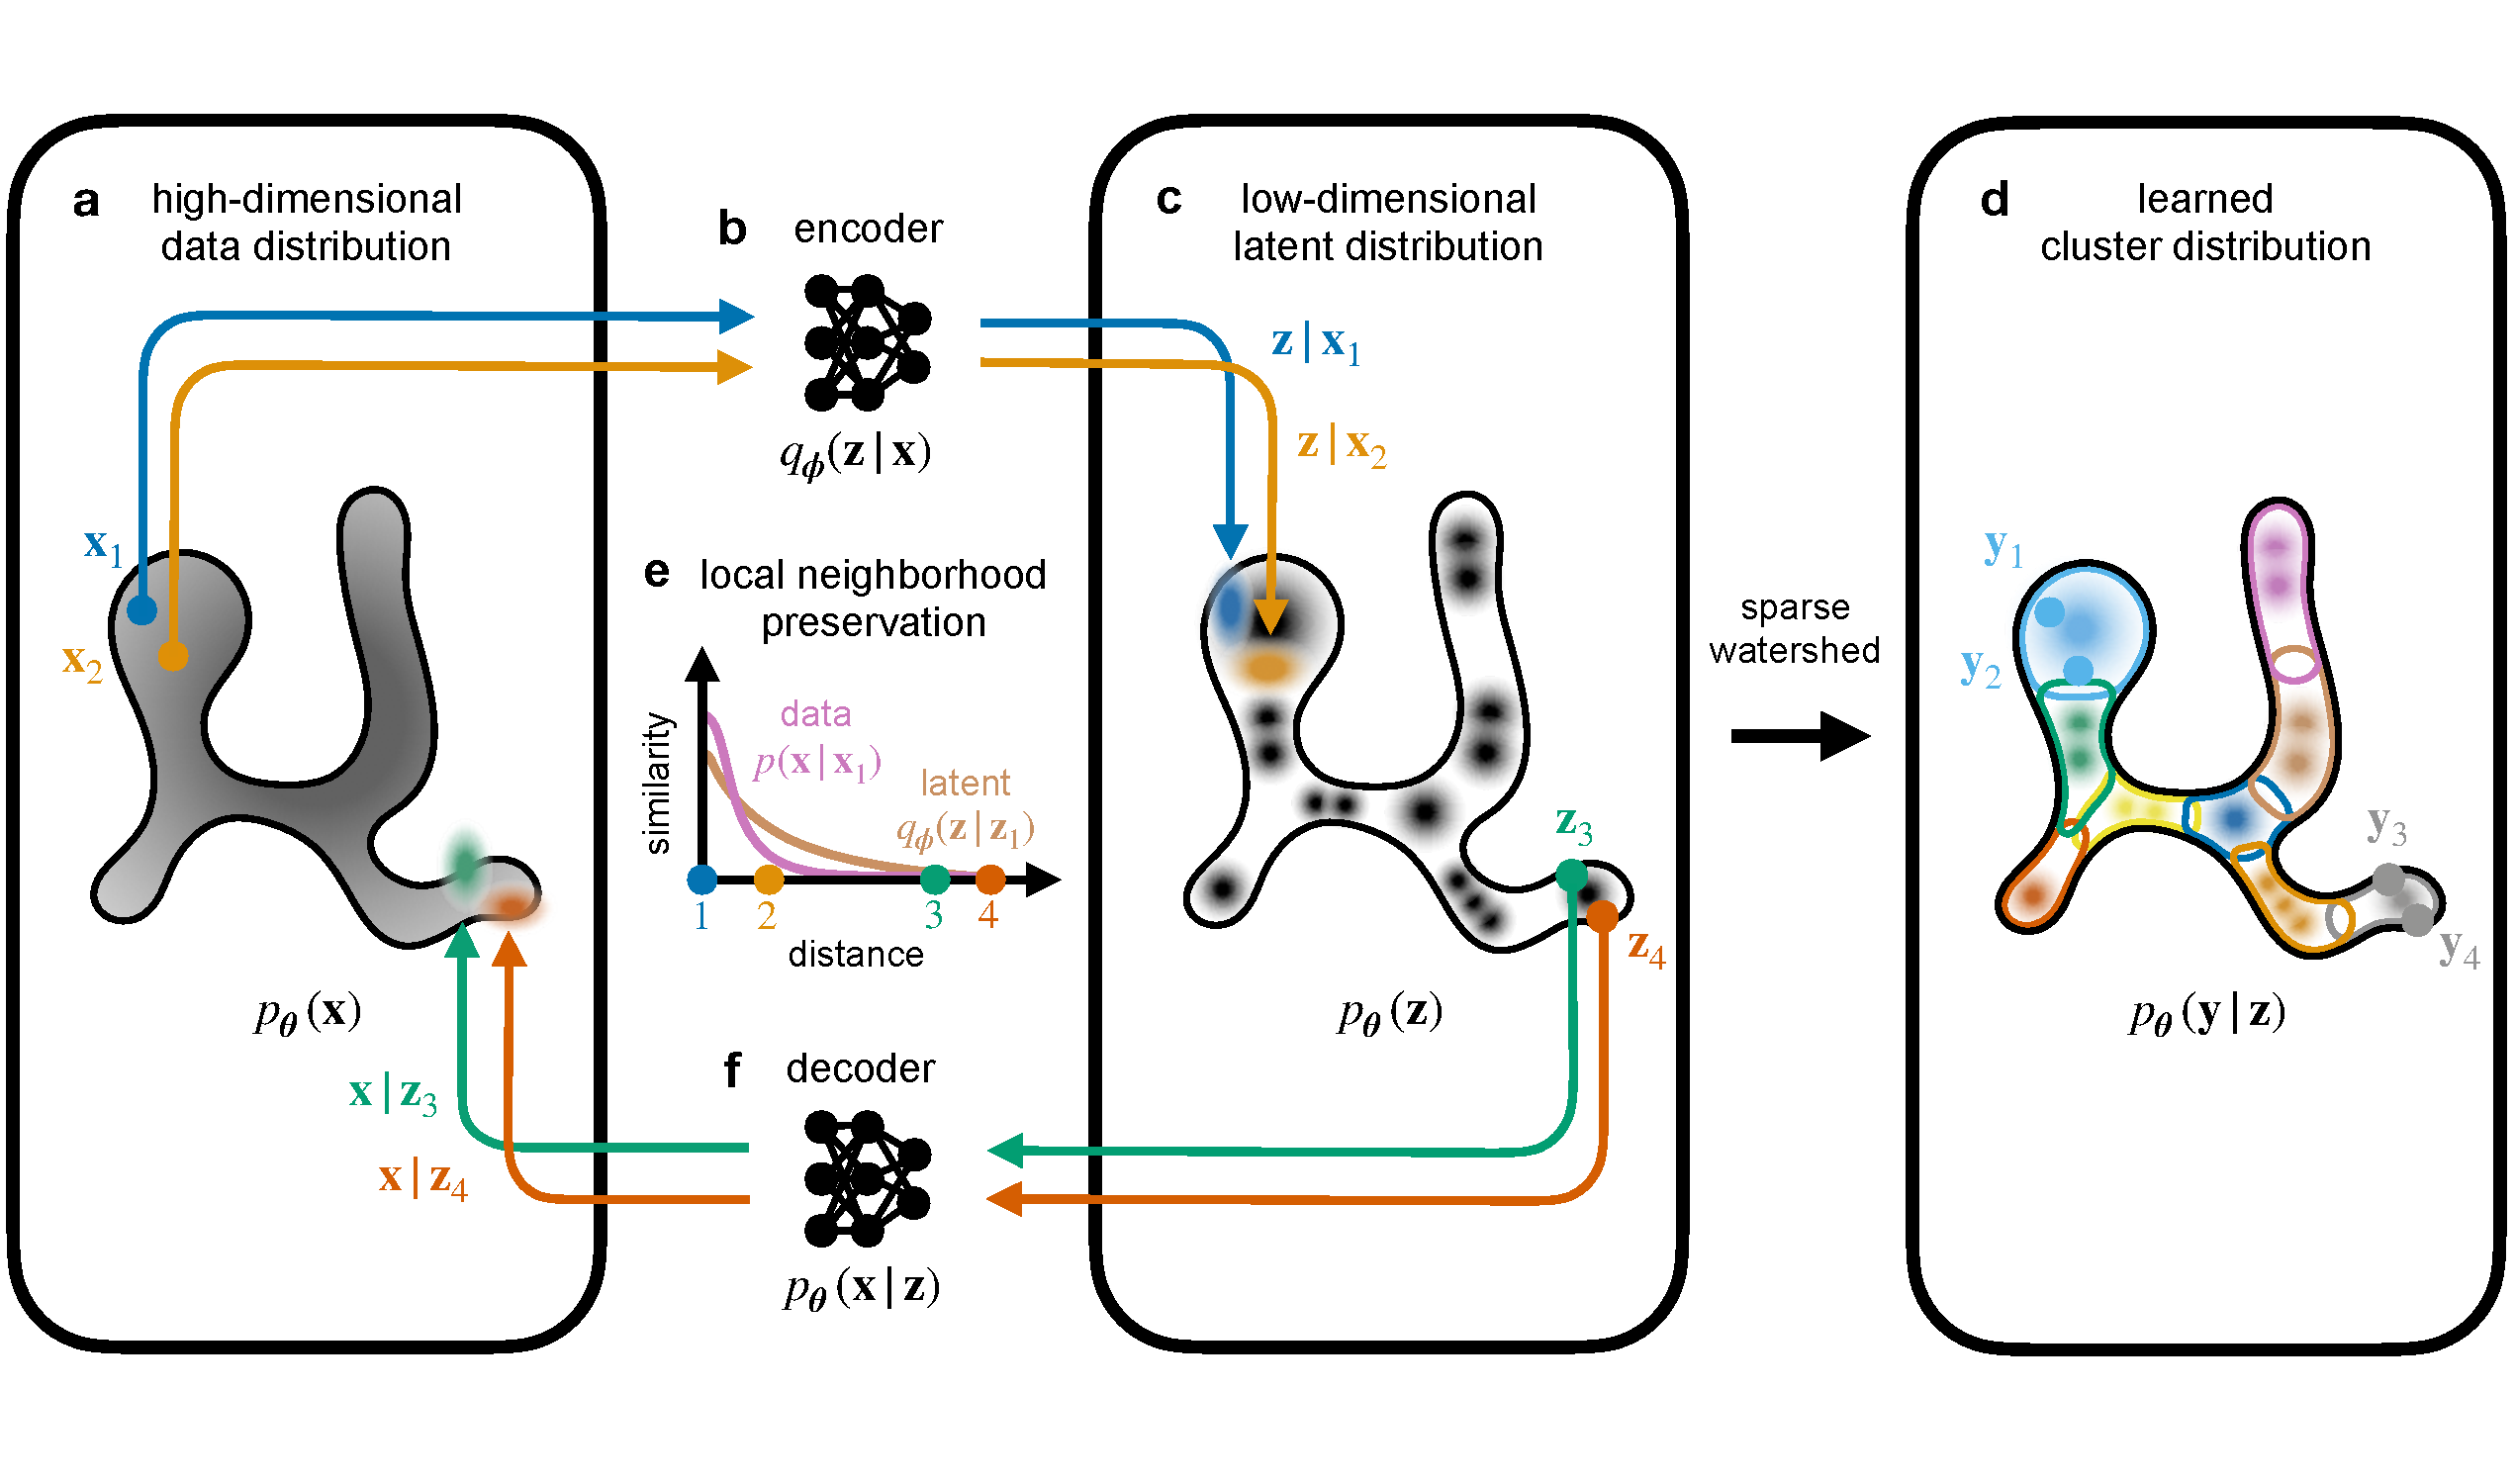
\includegraphics[width=\textwidth]{Graving_IMPRS_Thesis/figures/vaesne_figure.pdf}

\caption{  \textbf{Overview of the VAE-SNE model}. \textbf{a}-\textbf{f}, Observed samples from a high-dimensional data distribution $\mathbf{x} \sim p(\mathbf{x})$ (\textbf{a}) are probabilistically embedded (\textbf{b}) into a low-dimensional latent distribution $p_{\boldsymbol{\theta}}(\mathbf{z})$ (\textbf{c}) using an encoder deep neural network $\mathrm{DNN}_{\boldsymbol{\phi}}: \mathbf{x} \to \mathbf{z}$ to generate an approximate latent posterior distribution $q_{\boldsymbol{\phi}}(\mathbf{z} | \mathbf{x})$. Samples from the latent distribution $\mathbf{z} \sim q_{\boldsymbol{\phi}}(\mathbf{z} | \mathbf{x})$ or $\mathbf{z} \sim p_{\boldsymbol{\theta}}(\mathbf{z})$ (\textbf{c}) are then transformed (\textbf{f}) using a generative decoder deep neural network $\mathrm{DNN}_{\boldsymbol{\theta}}: \mathbf{z} \to \mathbf{x}$ to probabilistically reconstruct the high-dimensional data distribution $p_{\boldsymbol{\theta}}(\mathbf{x} | \mathbf{z})$. Given a set of observed high-dimensional data
$\{\mathbf{x}_1, \mathbf{x}_2, \dots, \mathbf{x}_N\}$ the model parameters for the encoder and decoder $\{\boldsymbol{\theta}, \boldsymbol{\phi}\}$ are optimized so that the approximate posterior for the encoder matches the true posterior from the generative decoder as best as possible, or $q_{\boldsymbol{\phi}}(\mathbf{z} | \mathbf{x}) \approx p_{\boldsymbol{\theta}}(\mathbf{z} | \mathbf{x})$, which then creates a functional mapping between the high-dimensional and low-dimensional distributions. To improve local structure preservation during optimization, pairwise distances between vectors in the high-dimensional and low-dimensional space are optimized using pairwise similarity kernels (\textbf{e}), a probability density function of distance, so that the local neighborhoods around each observation match as best as possible, or $p(\mathbf{x} | \mathbf{x}_i) \approx q_{\boldsymbol{\phi}}(\mathbf{z} | \mathbf{z}_i)$. This preferentially weights the preservation of local neighborhoods over global relationships by assigning more probability mass to nearby neighbors during optimization. The prior for the latent distribution $p_{\boldsymbol{\theta}}(\mathbf{z})$ is also a learned Gaussian mixture distribution (\textbf{c}) that is jointly optimized with the encoder and decoder to fit the observed data and can be used to cluster the latent distribution (\textbf{d}) into a small set of discrete classes $p_{\boldsymbol{\theta}}(\mathbf{y} | \mathbf{z})$ --- where highly-overlapping modes (mixture components) within the distribution are automatically merged into the same class label using sparse watershed assignment (Methods; \citealt{todd2017systematic})}

\label{fig:vaesne_figure} % \label works only AFTER \caption within figure environment

\end{figure}

\section{Results}
We make three main contributions in this paper: (\textbf{1}) First, we introduce a deep generative model for both dimensionality reduction and clustering called variational autoencoder stochastic neighbor embedding (VAE-SNE; Fig. \ref{fig:vaesne_figure}; Methods). VAE-SNE can produce a variety of different compressed representations and readily scales to out-of-core datasets with tens-of-millions of observations. Our model builds on numerous ideas from past work by synthesizing methods from a class of generative models known as variational autoencoders (VAEs; \citealt{kingma2013vae}), the popular dimensionality reduction algorithm (\textit{t}-distributed) stochastic neighbor embedding (SNE/t-SNE;\citealt{hinton2003stochastic, maaten2008tsne}) and its many extensions \citep{van2009ptsne, wang2016vmf, chien2017variational, ding2018scvis}, as well as recent advances in variational inference \citep{kingma2014semi, burda2015iwae, dilokthanakul2016gmvae, cremer2017reinterpreting, tomczak2017vae} and clustering methods \citep{todd2017systematic}. (\textbf{2}) Second, we apply VAE-SNE, and a variety of other popular dimensionality reduction methods, to compress real-world datasets from different domains (Fig. \ref{fig:embedded_data_figure}). We then quantitatively assess how each algorithm performs in preserving important aspects of the data --- including information about local, global, and temporal structure. We also assess generalization to new, out-of-sample data and compare processing speeds for each algorithm. Additionally, we show how the likelihood score produced by VAE-SNE can be used to detect outliers when embedding out-of-sample data. (\textbf{3}) Third, we show how VAE-SNE can be used to automatically cluster large datasets into a small set of interpretable classes. As a practical example, we apply VAE-SNE to a dataset of 21.1 million observations describing the high-dimensional body posture dynamics of a commonly-used model organism --- the fruit fly (\textit{Drosophila melanogaster}) --- to automatically discretize these data into motifs of stereotyped behavior for further analysis (Fig. \ref{fig:cluster_figure}; \citealt{berman2014mapping, pereira2019fast}). These results illustrate how VAE-SNE can be used as a type of automated ethogram for describing the full behavioral repertoire of animals (reviewed by \citealt{anderson2014toward, berman2018measuring, brown2018ethology, datta2019computational}), while also providing several advantages over existing methods for this task.


Our approach (Fig. \ref{fig:vaesne_figure}; Methods) builds on VAEs as a base model for performing dimensionality reduction (Appendix \ref{appendix:vae}), which, like other types of autoencoders \citep{hinton2006reducing}, model high-dimensional data using two deep neural networks: one to encode data to a compressed latent representation, and another to decode the latent vectors and reconstruct the data. However, VAEs are distinct from other autoencoders in that the encoder is used to parameterize continuous distributions of latent vectors --- from which latent vectors are then probabilistically sampled --- rather than embedding each high-dimensional observation as a single point in the latent space. This type of model offers an attractive dimensionality reduction framework because the objective function (Appendix \ref{appendix:elbo}) naturally imparts a trade-off between the complexity of the encoded description and the overall accuracy of the decoded reconstruction \citep{alemi2016deep}. However, these models suffer from multiple long-standing issues including a phenomenon known as \textit{posterior collapse} \citep{alemi2017fixing, dieng2019avoiding} where the latent coordinate space becomes arbitrarily organized and no longer preserves any statistical features of the high-dimensional data distribution. There has been a string of recent work to address these issues including some relatively straightforward solutions \citep{higgins2016beta, dieng2019avoiding} that achieve varying levels of success, as well as new objective functions that involve regularizing the mutual information between the high-dimensional data and latent distribution (e.g., \citealt{zhao2017infovae, rezaabad2019learning}; reviewed by \citealt{poole2019variational}). 

For VAE-SNE, we provide an effective solution to this problem with the addition of a stochastic neighbor regularizer (Appendix \ref{appendix:sne}; \citealt{maaten2008tsne, van2009ptsne, chien2017variational, ding2018scvis}) that optimizes pairwise similarity kernels between the high- and low-dimensional distributions to strengthen local neighborhood preservation and more explicitly retain a useful representation. We also draw on other theoretical and practical improvements from the literature to enhance the performance of VAE-SNE (Methods). For example, we use a Gaussian mixture prior for learning the latent distribution \citep{kingma2014semi, dilokthanakul2016gmvae, tomczak2017vae}. This choice of distribution allows for better local structure preservation and, when combined with sparse watershed assignment to merge overlapping mixture components (Fig. 
\ref{fig:vaesne_figure}; Methods; \citealt{todd2017systematic}), serves as a flexible method for clustering data --- without the need to manually define the number of clusters or impose strong assumptions about cluster shape. We employ several other advances to further improve structure preservation. For instance, we apply a perplexity annealing technique \citep{kobak2019art} to slowly decay the size of the local neighborhoods optimized by the model during training, which helps to preserve structure across multiple scales. Moreover, we extensively optimize the algorithms underlying our model by applying parallel computations on the CPU and GPU that dramatically improve processing speed compared to previous work \citep{ding2018scvis}.

In addition to our three main contributions, we further extend VAE-SNE to demonstrate its flexibility as a framework for dimensionality reduction. To accomplish this, we introduce a von Mises-Fisher variant of VAE-SNE (Appendix \ref{appendix:spherical}; Fig. \ref{fig:spherical_figure}; \ref{fig:spherical_embedding_posture_video}, \ref{fig:spherical_embedding_rna_video}) that embeds data in polar coordinates (rather than Euclidean coordinates) on a 3-D unit sphere, which is potentially a more natural representation for many high-dimensional datasets \citep{davidson2018hyperspherical} and solves the ``crowding" problem common to some methods \citep{maaten2008tsne, ding2019deep}. Finally, we also apply a modified convolutional version of VAE-SNE (Appendix \ref{appendix:conv}; Figs. \ref{fig:shell_figure}, \ref{fig:butterfly_figure}) to visualize natural history images of animal specimen collections \citep{cuthill2019deep, zhang2019shell} by directly embedding the raw pixel data. Our results for these two extensions are described in Appendix \ref{appendix:extensions}.


\subsection{Comparisons with other dimension reduction algorithms}
Current methods for dimensionality reduction generally fall into two classes known as \textit{linear} and \textit{nonlinear} algorithms. Linear algorithms, such as principal components analysis (PCA), compress high-dimensional data by learning linearly weighted combinations (affine transformations) of the original feature set. Typically these algorithms are optimized to preserve the global structure of the data, where local neighborhood relationships are distorted in order to maintain the full coordinate system of the original features as best as possible. On the other hand, nonlinear algorithms (sometimes called manifold learning algorithms) such as t-SNE (\citealt{maaten2008tsne}) and uniform manifold approximation and projection (UMAP; \citealt{mcinnes2018umap}) typically take the opposite approach of prioritizing relative relationships between data points rather than the global coordinate system. This approach allows local neighborhoods to be preserved while potentially sacrificing information about the larger-scale relationships between data points in the global coordinate space --- although, as we demonstrate here, the global distortion imposed by many of these algorithms is actually comparable to that of PCA.

To validate VAE-SNE as a general-purpose method for  dimensionality reduction, we quantitatively compare its performance with other dimension reduction algorithms --- both linear and nonlinear --- using two datasets from different domains (see Methods) describing animal body part dynamics \citep{berman2014mapping, berman2016predictability, pereira2019fast} and single-cell RNA-seq expression profiles for hippocampal neurons \citep{la2018rna}. We benchmark multiple variants of VAE-SNE with different pairwise similarity kernels for preserving local neighborhood information (including kernel functions with learned parameters; Appendix \ref{appendix:sne}), and we compare these results with those from two high-performance variants of t-SNE \citep{maaten2008tsne} known as FIt-SNE \citep{linderman2017efficient, linderman2019fast} and Barnes-Hut-SNE \citep{van2014accelerating}, as well as UMAP \citep{mcinnes2018umap}, and two other deep neural network-based dimension reduction methods: scvis \citep{ding2018scvis}, and ivis \citep{szubert2019ivis}. We also apply PCA in 2, 5, 10, and 100 dimensions for a linear baseline comparison. We fit each algorithm with a training set and also embed an out-of-sample test set to assess generalization to new data. For both the training and test sets, we then quantitatively assess each algorithm's ability to preserve different types of information about the high-dimensional data when compressing the data to two dimensions, including local, global, fine-scale, and temporal information (Methods). We quantify local information preservation for each algorithm by measuring the preservation of both metric (distance- or radius-based) and topological (nearest neighbors-based) neighborhoods that are approximately $1\%$ of the total embedding size; we measure global information preservation by calculating the correlation between pairwise distances in high- and low-dimensional space; we assess fine-scale information by measuring neighborhood preservation for multiple neighborhood sizes $<1\%$ of the total embedding size; and we evaluate temporal information preservation by computing the correlation between high- and low-dimensional temporal derivatives in a timeseries dataset.  Overall the qualitative properties of the embeddings produced by each algorithm are strikingly similar within datasets (Fig. \ref{fig:embedded_data_figure}), which likely indicates shared mathematical properties of how the latent distributions are modelled. However, we do find potentially important quantitative differences between these algorithms in terms of information preservation and processing speed. We summarize our overall assessments of each nonlinear dimension reduction algorithm in Tables \ref{table:info}, \ref{table:speed}, \ref{table:features}.

\begin{figure}[!htb]
\centering
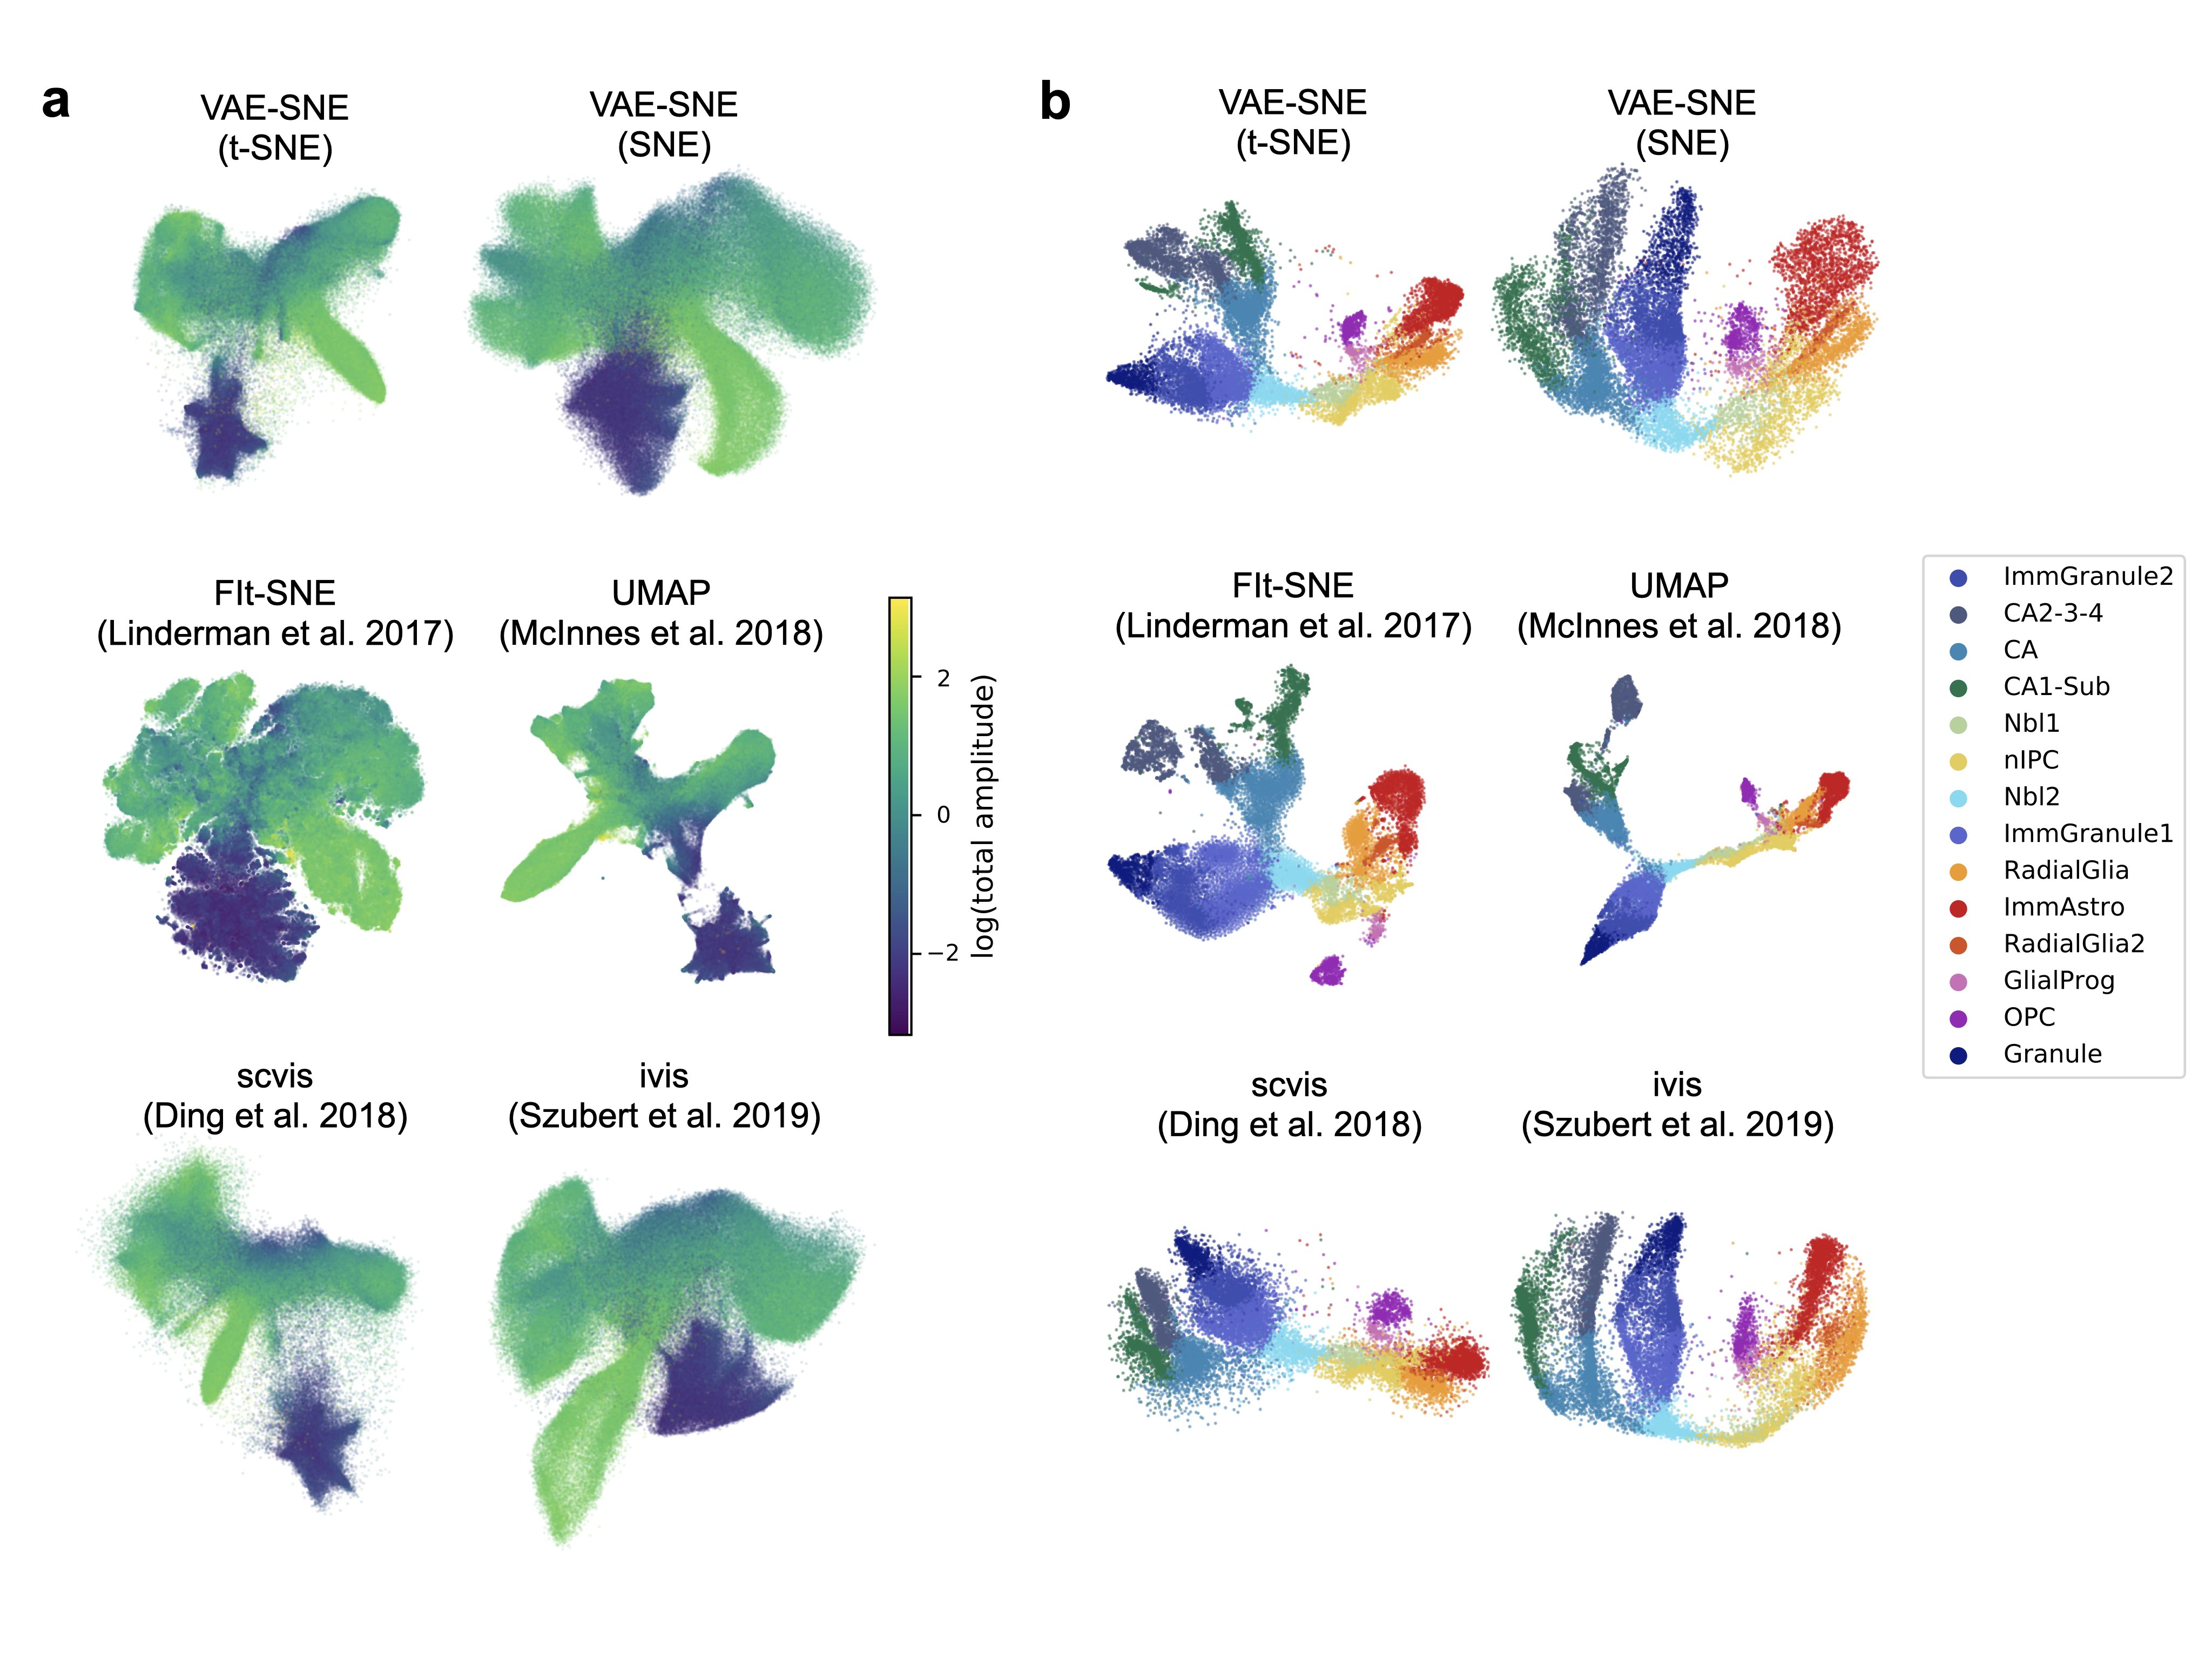
\includegraphics[width=1\textwidth]{Graving_IMPRS_Thesis/figures/embedded_data_figure.jpeg}

\caption{  \textbf{Embeddings for body posture dynamics and single-cell RNA-seq data.} \textbf{a}, 2-D embeddings of body posture dynamics data from \cite{berman2014mapping, berman2016predictability, pereira2019fast} for each algorithm we tested. The color of each point indicates the logarithm of the total amplitude (overall movement) of body parts for each observation. \textbf{b}, 2-D embeddings of single-cell RNA-seq data of developing hippocampal neurons from \cite{la2018rna} for each algorithm. The color of each point indicates the cell type for that observation as described by \cite{la2018rna}.}

\label{fig:embedded_data_figure} % \label works only AFTER \caption within figure environment

\end{figure}

\subsubsection{Local structure preservation}
We find that VAE-SNE compares closely to FIt-SNE \citep{linderman2017efficient}, Barnes-Hut-SNE \citep{van2014accelerating}, and UMAP \citep{mcinnes2018umap} in preserving local structure for both the training set (Figs. \ref{fig:training_set_figure}a, \ref{fig:training_set_appendix_figure}a, \ref{fig:rna_velocity_figure}a) and test set (Figs. \ref{fig:test_set_figure}a, \ref{fig:test_set_appendix_figure}a), while scvis \citep{ding2018scvis} and ivis \citep{szubert2019ivis} perform slightly worse. Our results show that VAE-SNE with a t-SNE similarity kernel \citep{maaten2008tsne} performs the best for preserving local structure, but VAE-SNE with a Gaussian SNE kernel \citep{hinton2003stochastic} also performs well --- similarly to scvis \citep{ding2018scvis} and ivis \citep{szubert2019ivis}. We also find that learning the similarity kernel parameters (for both Gaussian and Student's \textit{t} kernels) as a function of each data point does not improve performance for our local preservation metrics. The top performing algorithms for local structure preservation (VAE-SNE, t-SNE, and UMAP) are closely comparable to 5-dimensional PCA for both metrics we used to assess local neighborhood preservation.

\subsubsection{Global structure preservation}
We find that VAE-SNE also does well in preserving global structure for both the training set (Figs. \ref{fig:training_set_figure}a, \ref{fig:training_set_appendix_figure}b, \ref{fig:rna_velocity_figure}a) and test set (Figs. \ref{fig:test_set_figure}a, \ref{fig:test_set_appendix_figure}b). VAE-SNE with a Gaussian SNE kernel performs best for this metric, but VAE-SNE with a t-SNE kernel also performs nearly as well. Notably all the neural-network-based methods (VAE-SNE, scvis \citealt{ding2018scvis}, ivis \citealt{szubert2019ivis}) outperform both t-SNE and UMAP \citep{mcinnes2018umap} in preserving global structure for both datasets we tested. This is perhaps not surprising given that recent work has shown neural network models tend to learn the same axes as PCA \citep{rolinek2019variational}. Additionally, these results show that learning the similarity kernel parameters as a function of each data point does improve global structure preservation for VAE-SNE with a t-SNE kernel --- likely because it is optimized to be more similar to the Gaussian kernel used to calculate high-dimensional similarities (Appendix \ref{appendix:sne}). The top performing algorithms for this metric are comparable to 2-dimensional PCA, which demonstrates that nonlinear algorithms are capable of preserving the same global information as PCA while also better preserving local structure. On one hand, the scvis \citep{ding2018scvis} algorithm in particular excels at preserving global structure for the single-cell RNA-seq dataset we tested (Fig. \ref{fig:rna_velocity_figure}a), while, on the other hand, ivis \citep{szubert2019ivis} performs much more poorly than the other neural network algorithms for this dataset, and FIt-SNE \citep{linderman2017efficient, linderman2019fast} and Barnes-Hut-SNE \citep{van2014accelerating} perform even worse. We also show that UMAP \citep{mcinnes2018umap} with PCA initialization better preserves global structure than the default Laplacian Eigenmap initialization.

\subsubsection{Fine-scale structure preservation}
In addition to local and global structure preservation, we evaluate the ability of each algorithm to preserve very fine-scale neighborhood information (Figs. \ref{fig:training_set_figure}b, \ref{fig:test_set_figure}b, \ref{fig:rna_velocity_figure}b). We find that both FIt-SNE \citep{linderman2017efficient} and Barnes-Hut-SNE \citep{van2014accelerating} excel at preserving this fine-scale information for the posture dynamics dataset (Figs. \ref{fig:training_set_figure}b, \ref{fig:test_set_figure}b) while every other nonlinear algorithm performs relatively poorly for both the training and test set. For the single-cell RNA-seq dataset, this distinction is not nearly as large and the algorithms all perform more similarly (Fig. \ref{fig:rna_velocity_figure}b), which indicates performance varies depending on the dataset. Performance for the ivis algorithm \citep{szubert2019ivis} is especially poor for this metric on the single cell RNA-seq dataset. However, neighborhood membership for neighborhoods between $1\%$ and $10\%$ of the total embedding size are all similarly well-preserved for each algorithm.

\subsubsection{Temporal structure preservation}
 Because one of the datasets we use for benchmarking is a behavioral timeseries, for these data we also assess the temporal structure preservation of each algorithm (Figs. \ref{fig:test_set_figure}a, \ref{fig:test_set_appendix_figure}c) on the out-of-sample test set (the training set is randomly sampled across multiple timeseries, so temporal information is not preserved). We find that VAE-SNE (particularly the SNE kernel variant), FIt-SNE \citep{linderman2017efficient}, Barnes-Hut-SNE \citep{van2014accelerating}, scvis \citep{ding2018scvis}, and ivis \citep{szubert2019ivis} perform at the same level as 5-dimensional PCA in preserving temporal structure, while UMAP \citep{mcinnes2018umap} performs relatively poorly in comparison to the other algorithms --- even worse than 2-dimensional PCA.

\subsubsection{Speed comparisons}
In addition to assessing information preservation, we also compare the speed the of each algorithm both when fitting the algorithm to the training set (Figs. \ref{fig:training_set_figure}c, \ref{fig:rna_velocity_figure}c) and when embedding an out-of-sample test set (Figs. \ref{fig:test_set_figure}c, \ref{fig:rna_velocity_figure}c). We find that training time increases approximately linearly with the size of the dataset for each algorithm. UMAP \citep{mcinnes2018umap} has the fastest training time (approximately as fast as PCA), followed by FIt-SNE \citep{linderman2017efficient} and Barnes-Hut-SNE \citep{van2014accelerating}, and then VAE-SNE. While VAE-SNE is slower for fitting the training set than both UMAP \citep{mcinnes2018umap} and t-SNE, it is much faster than the other two neural network methods scvis \citep{ding2018scvis} and ivis \citep{szubert2019ivis}. We also demonstrate that VAE-SNE, and the other neural network methods, can quickly embed out-of-sample test data (Figs. \ref{fig:test_set_figure}c, \ref{fig:rna_velocity_figure}c). The time needed for embedding new data is much higher for both t-SNE and UMAP, and while the elapsed time for embedding the test set scales linearly with the number of samples for all algorithms, we also find that it increases with the size of the training set for both UMAP \citep{mcinnes2018umap} and Barnes-Hut-SNE \citep{van2014accelerating}  (Fig. \ref{fig:test_set_figure}c). This is almost certainly because adding new data for these algorithms requires calculating approximate nearest neighbors between the out-of-sample data and the training set, which consequently requires more computation time for larger training sets. Unexpectedly, FIt-SNE \citep{linderman2017efficient} does not exhibit this behavior despite using similar nearest neighbor calculations to Barnes-Hut-SNE \citep{van2014accelerating}. On the other hand, VAE-SNE and other deep learning algorithms do not suffer from this limitation. Finally, while we do not comprehensively assess memory complexity of different algorithms in this paper, we stopped our speed comparisons at data subsets with 232,000 ($\times$ 1500 dimensions) observations because UMAP began to cause out-of-memory errors for larger subsets --- while all of the other algorithms we tested could still successfully run under the same conditions. This helps to illustrate the key advantage of deep learning-based methods, which naturally maintain very low memory complexity by applying optimization using small batches of data.

\subsection{Using the likelihood to assess out-of-sample data}
Because VAE-SNE also calculates a likelihood score for reconstructing the original high-dimensional data, we can use this to assess performance on out-of-sample data, which is an idea originally proposed by \cite{ding2018scvis}. To test this, we calculate the likelihood score for real data from the posture dynamics dataset \citep{berman2014mapping, berman2016predictability, pereira2019fast} and randomly-permuted data (randomized across feature columns) from the same dataset. We find that the likelihood score is reliably lower for the randomized data, and the two likelihood distributions are well separated (Fig. \ref{fig:likelihood_entropy_figure}a), which shows this metric could potentially be used to detect outliers. We also compare the entropy of the approximate posterior distribution for each embedded sample as another potential metric for detecting outliers. While we find that the entropy is much higher for the randomized data, the distribution is highly overlapping with the entropy for the real data (Fig. \ref{fig:likelihood_entropy_figure}b), which indicates the entropy may not be as useful for evaluating the embedding quality.

\begin{figure}[!htb]
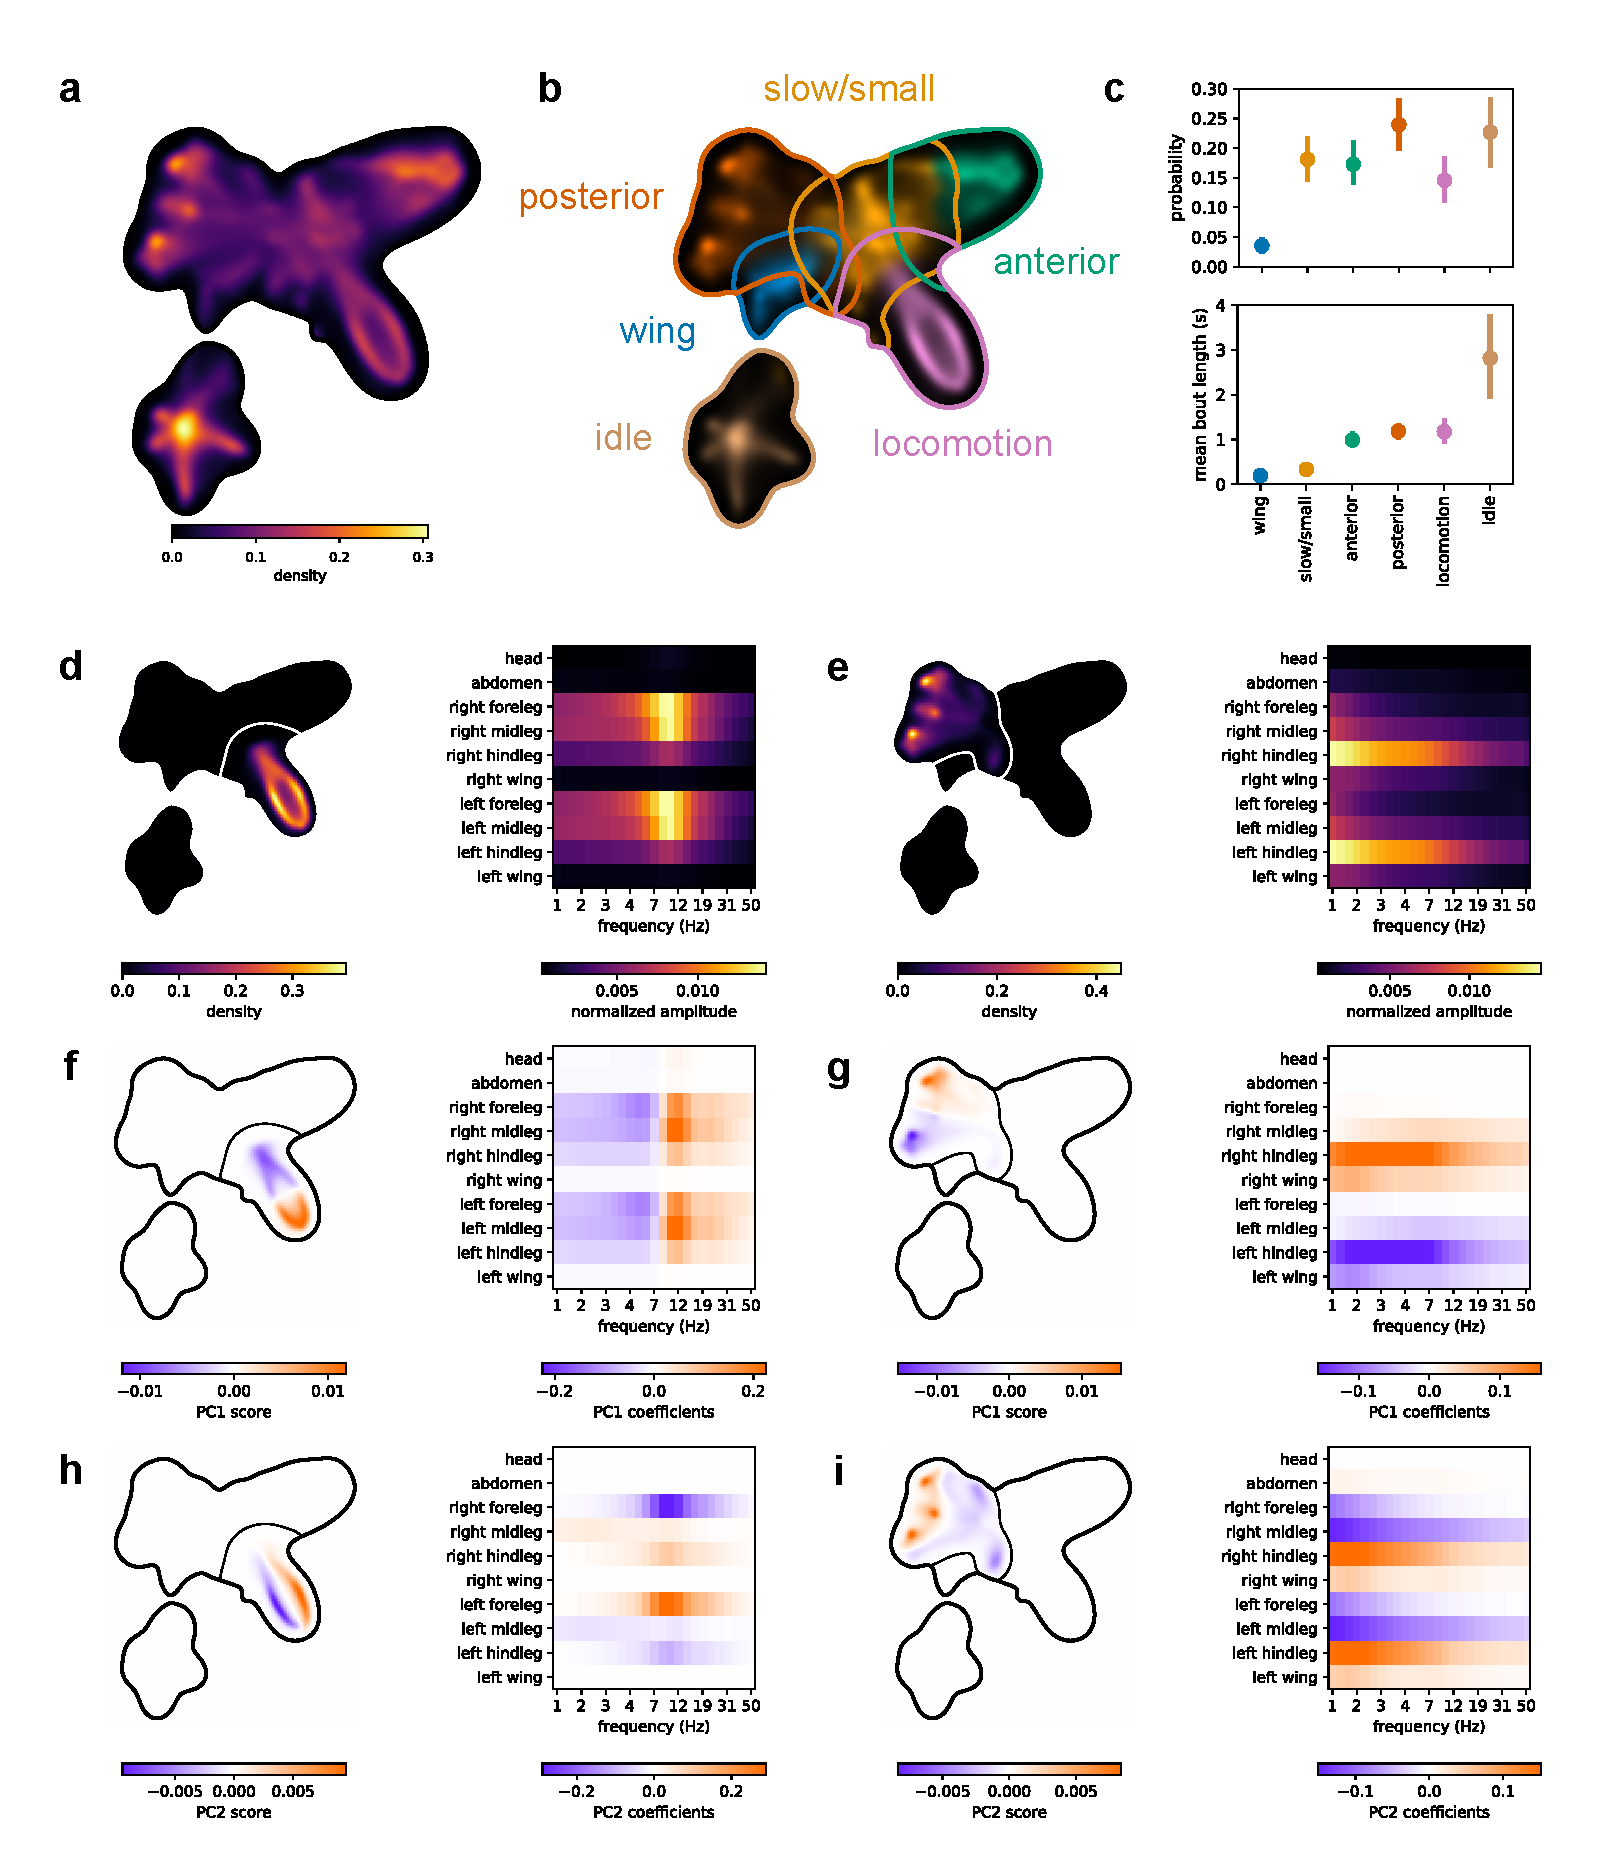
\includegraphics[width=0.9\textwidth]{Graving_IMPRS_Thesis/figures/cluster_figure.pdf}
\centering

\caption{  \textbf{Clustering body posture dynamics.} \textbf{a}, The posterior probability density for the full 21.1 million observation body posture dynamics dataset from \cite{berman2014mapping, berman2016predictability, pereira2019fast} embedded using a 2-dimensional VAE-SNE model. \textbf{b}, The manually-grouped high-level cluster assignments produced using the learned prior from a 30-dimensional VAE-SNE embedding visualized in the 2-D embedding, where contours are the largest 90\% probability density contour for each cluster distribution. \textbf{c}, Mean and 95\% bootstrap intervals of the marginal (stationary) probability and mean bout length for each high-level cluster (n = 59 per cluster). \textbf{d}-\textbf{i}, Visualizations describing the high-level locomotion (\textbf{d},\textbf{f},\textbf{h}; \ref{fig:locomotion_video}; Fig. \ref{fig:locomotion_cluster_figure}) and posterior grooming (\textbf{e},\textbf{g},\textbf{i}; \ref{fig:posterior_video}; Fig. \ref{fig:posterior_cluster_figure}) clusters. \textbf{d-e}, The 2-D posterior probability density for each cluster (left) and the mean spectrogram for each cluster (right). \textbf{f}-\textbf{i}, The principal component scores for the two largest components of the spectrograms assigned to each cluster visualized within the 2-D embedding (left), and the eigenvector coefficients describing the linear contribution of each spectrogram feature (right) for the principal component score.}
\label{fig:cluster_figure}
\end{figure}


\subsection{Clustering body posture dynamics to reveal stereotyped behavioral organization}
To demonstrate its capabilities as a clustering algorithm, we use VAE-SNE to automatically discretize a dynamical timeseries dataset describing the high-dimensional body posture and behavioral repertoire of 59 freely-behaving fruit flies (\textit{D. melanogaster}; \citealt{berman2014mapping, berman2016predictability, pereira2019fast}) --- a commonly-used model organism for neuroscience, pharmaceutical, and genetics research. To accomplish this, we use the annotated training data from \citep{pereira2019fast} to train a pose estimation model using deep learning-based software (DeepPoseKit; \citealt{graving2019deepposekit}). We then use this trained model to automatically track the spatial locations of 10 body parts (head, legs, wings, abdomen) directly from video timeseries data and generate time-frequency spectrograms describing body-part dynamics for each observation in the timeseries \citep{berman2014mapping}, which naturally incorporates multi-scale temporal information into each data vector. We then apply VAE-SNE to compress the data to a 30-dimensional latent embedding and simultaneously discretize the dynamical posture timeseries into a set of behavioral clusters. We find that, after optimizing the 30-D VAE-SNE model for 5 repeated trials using the full 21.1 million observation dataset and applying sparse watershed assignment to generate cluster labels (Methods; Fig. \ref{fig:vaesne_figure}d; \citealt{todd2017systematic}), VAE-SNE consistently learns a total of 26 low-level behavioral clusters describing distinct, stereotyped body part movements. We also achieve similar (nearly identical) results when clustering in 10-D and 50-D space and when varying the number of components in the Gaussian mixture prior used for clustering --- provided that the number of components is large enough (e.g., $K \geq 100$).

To provide a broad overview of the behavioral structure discovered by VAE-SNE, we manually group these low-level clusters into 6 high-level clusters (Figs. \ref{fig:cluster_figure}, \ref{fig:cluster_appendix_figure}; \ref{fig:sequences_video}) by examining video clips sampled from each cluster (\ref{fig:locomotion_video}--\ref{fig:idle_video}) and by calculating and visualizing the mean spectrograms for each low-level cluster to quantify the average distribution of body part movements across frequencies for each behavioral class (Figs. \ref{fig:locomotion_cluster_figure}d-f, \ref{fig:posterior_cluster_figure}d-i). These high-level clusters include: locomotion (\ref{fig:locomotion_video}), anterior grooming (\ref{fig:anterior_video}), posterior grooming (\ref{fig:posterior_video}), wing movements (\ref{fig:wing_video}), small/slow leg movements (\ref{fig:slow_video}), and idle behavior (\ref{fig:idle_video}). Many of the low-level clusters (10 clusters in total) describe distinct slow/small leg movements, while there are 3 low-level clusters for locomotion (Fig. \ref{fig:locomotion_cluster_figure}), 3 for anterior grooming, 6 for posterior grooming (Fig. \ref{fig:posterior_cluster_figure}), 2 for wing movements, and 2 for idle behavior. Videos and posture timeseries data sampled from each cluster also clearly demonstrate the stereotypy of behaviors within these behavioral classes, which matches well with previous work describing these dynamics \citep{berman2014mapping, berman2016predictability, klibaite2017unsupervised, klibaite2019interacting, pereira2019fast}. Additionally, the principal components of the spectrograms from each high-level cluster (Fig. \ref{fig:cluster_figure}f-i; Fig. \ref{fig:cluster_appendix_figure}d-i) reveal continuous variation related to asymmetrical body movements and differences in peak movement frequency. We calculate basic statistics describing cluster usage across individuals (Figs. \ref{fig:cluster_figure}c, \ref{fig:locomotion_cluster_figure}c, \ref{fig:posterior_cluster_figure}c) including the marginal (stationary) probability of behavioral classes and the mean bout length, or the average amount of time a behavior is performed when an individual transitions into that cluster. In particular, the low probability and short bout length for wing movements and short bout length for slow/small leg movements (Fig. \ref{fig:cluster_figure}c) indicate these clusters may be transitional or idiosyncratic behaviors \citep{todd2017systematic}. For the low-level locomotion clusters (Fig. \ref{fig:locomotion_cluster_figure}) we also calculate the forward component of the leg movement velocity (in body lengths per second, or $\textrm{BL} \cdot \textrm{s}^{-1}$) relative to the egocentric orientation of the animal. We then use the forward velocity to classify each leg in the timeseries as ``swing" (forward velocity $> 0 \, \textrm{BL} \cdot \textrm{s}^{-1}$) or ``stance" (forward velocity $\leq 0 \, \textrm{BL} \cdot \textrm{s}^{-1}$) and find that our low-level locomotion clusters show signatures of distinct locomotory gaits (i.e., tetrapod and tripod gaits; \citealt{mendes2013quantification, pereira2019fast}) with different numbers of legs being used for walking, on average, within each cluster. Together these results demonstrate that VAE-SNE is able to automatically decompose the dynamics of known complex behaviors (\ref{fig:sequences_video}).

Due to the many philosophical complexities of objectively evaluating unsupervised cluster representations (reviewed by \citealt{jain1999data, kleinberg2003impossibility, todd2017systematic}), we forgo any further quantitative assessment of our clustering results and instead leave this for future work. For example, it is unclear how to best select the number of clusters for many different algorithms; how to properly compare algorithms that naturally produce different numbers of clusters and cluster shapes; and what metric(s) should be used to meaningfully evaluate a clustering description as generally ``good" or ``useful" other than manual, qualitative validation of the results, which we already provide here --- though several quantitative descriptors with varying levels of desirability have been recently proposed for behavioral data \citep{todd2017systematic}. Comparing unsupervised cluster labels with a priori-defined labels --- as is common practice (e.g., \citealt{jiang2016variational, xie2016unsupervised, guo2017improved, yang2019deep, luxem2020identifying}) --- is also problematic, as human-supervised descriptions may not accurately capture the underlying structure of the data distribution, and this is especially true for datasets where the goal is to potentially discover subtle differences that are undetectable by humans (e.g., \citealt{wiltschko2015mapping}). Despite the limitations imposed by these complexities, our results still illustrate multiple useful features of VAE-SNE as a general-purpose method.

Overall, we demonstrate how VAE-SNE can be used as a practical, scalable, and flexible tool for clustering real-world high-dimensional data. In this case, we transform posture data into interpretable behavioral labels that are comparable to those from previous methods \citep{berman2014mapping, berman2016predictability, todd2017systematic, klibaite2017unsupervised, cande2018optogenetic, klibaite2019interacting, pereira2019fast}. However, in contrast to many of these existing methods, VAE-SNE performs dimension reduction and clustering simultaneously, and unlike most previously-described algorithms for clustering data (e.g., \citealt{jiang2016variational, xie2016unsupervised, guo2017improved, yang2019deep}), our method learns a small set of decipherable classes without the need to carefully tune the number of clusters fitted to the data, which can often be a non-trivial, unintuitive, and computationally-intensive process \citep{milligan1985examination, pham2005selection, fang2012selection, todd2017systematic}. Instead, any arbitrarily large number will give similar results due to the sparse watershed assignment procedure we use to combine overlapping clusters (Methods; Fig. \ref{fig:vaesne_figure}d; \citealt{todd2017systematic}). 
In contrast to methods that impose strong assumptions about cluster shape, our clustering method has relaxed assumptions and allows for more complex (e.g., non-convex) cluster distributions based on the local structure of the data. 
Additionally, in comparison to prior methods for unsupervised behavioral analysis, VAE-SNE has the advantage of being able to use more than two dimensions for clustering data, which has been shown to provide higher-quality behavioral labels with many potentially-desirable properties \citep{todd2017systematic}. Finally, our results further show that there is no need to carefully select a subset of data to use for training (e.g., the importance sampling technique described by \citealt{berman2014mapping}), which can also be a time-consuming process. Instead, VAE-SNE can be readily applied to large datasets that cannot fit into memory while still successfully detecting relatively short-lived and infrequent types of behavior, such as wing movements (Fig. \ref{fig:cluster_figure}b-c; \ref{fig:wing_video}).

\section{Discussion}
Here we introduce VAE-SNE, a deep generative model for simultaneously reducing dimensionality and clustering data. We compare VAE-SNE to existing methods for dimensionality reduction and demonstrate its utility and versatility using real-world examples. Our results establish that VAE-SNE is able to generate robust and interpretable compressed representations for data from different domains and is comparable in performance to other nonlinear methods for dimensionality reduction. In contrast to these existing methods, VAE-SNE has the advantage of being able to automatically cluster similar observations into a small set of classes, which can then be used to summarize large datasets with coarse-grained descriptors or select specific subpopulations of data for more detailed analysis. Our approach can also readily scale to very large datasets by leveraging techniques from deep learning --- including, and especially, out-of-core data that cannot fit into memory. However, despite these strengths, VAE-SNE still has important limitations depending on the goals of the user, and there are many ways in which the model could be improved or extended in subsequent iterations. There are also other domains that VAE-SNE could be applied to in the future.

VAE-SNE preserves local relationships while also minimizing global structure distortion. Additionally, while VAE-SNE is not explicitly an autoregressive model, it still preserves a good deal of high-dimensional timeseries information. However, our results also show that VAE-SNE, and most of the other dimension reduction methods we tested, does not accurately preserve fine-scale structure (neighborhoods $<$1\% of the total embedding size). For many applications, preserving these details may be unimportant, but this structure has been shown to be useful for detecting infrequent types of data, such as rare cell types \citep{linderman2019fast}. Therefore, our results suggest that if researchers wish to preserve this type of information they should use FIt-SNE \citep{linderman2017efficient, linderman2019fast} or Barnes-Hut-SNE \citep{van2014accelerating} over other algorithms for dimension reduction. We also find that, when initialized with PCA over the default initialization, UMAP \citep{mcinnes2018umap} preserves global structure slightly better without noticeably affecting local structure preservation, so PCA may be a more advantageous choice for initializing UMAP embeddings.

VAE-SNE optimizes faster than existing deep learning methods for dimensionality reduction, but FIt-SNE \citep{linderman2017efficient, linderman2019fast}, Barnes-Hut-SNE \citep{van2014accelerating}, and UMAP \citep{mcinnes2018umap} are still faster. However, the training time for deep-neural-network methods like VAE-SNE and ivis \citep{szubert2019ivis} can be variable due to the use of early stopping criteria that automatically end training when no improvement in the objective function is detected. These early stopping criteria could be easily adjusted to further shorten (or lengthen) training time. While we did not assess performance during the optimization process, much of the training time for VAE-SNE is spent on minor improvements to the objective function, which indicates adequate results can also be achieved with less training time. Additionally, FIt-SNE \citep{linderman2017efficient, linderman2019fast}, Barnes-Hut-SNE \citep{van2014accelerating}, and UMAP \citep{mcinnes2018umap}, are much slower for embedding new data because they calculate nearest neighbors for the new data and further optimize the embedding, which VAE-SNE does not require due to its learned encoder function. For smaller datasets that can fit in memory FIt-SNE \citep{linderman2017efficient, linderman2019fast}, Barnes-Hut-SNE \citep{van2014accelerating}, and UMAP \citep{mcinnes2018umap} are still attractive options for dimensionality reduction, but for datasets that do no fit into memory, VAE-SNE provides some distinct advantages.

VAE-SNE has the ability to detect outliers and assess the embedding quality for out-of-sample data. This provides a straightforward mechanism for identifying new data to include in the training set, which can further improve performance. Most of the other algorithms we tested, or at least the specific software implementations we tested, provide no mechanism for quantitatively assessing embedding quality for each observation --- with outliers being simply embedded under the assumption that the data are well supported by the training distribution. This can cause problems for any downstream analysis, especially when using statistical tests to answer scientific questions. Further improvements for outlier detection might include the use of Bayesian inference \citep{hafner2018reliable} or other methods for estimating predictive uncertainty (reviewed by \citealt{kendall2017uncertainties}). 

We demonstrate that results produced by VAE-SNE can serve as a highly-interpretable coarse-grained description of tens-of-millions of observations --- with several advantages over existing methods for clustering data. Applying VAE-SNE to future research in the behavioral sciences could help to reveal the genetic, environmental, and neural underpinnings of animal behavior \citep{berman2018measuring, brown2018ethology, datta2019computational} --- especially when combined with recent advances in behavioral measurement \citep{mathis2018deeplabcut, pereira2019fast, graving2019deepposekit, gunel2019deepfly3d} as well as genetic \citep{ran2013genome,doudna2014new}, sensory \citep{stowers2017virtual}, and neural \citep{bath2014flymad, cande2018optogenetic} manipulations. The clustering capabilities of VAE-SNE could also be applied to other types of data, such as single-cell RNA-seq data \citep{ding2018scvis, la2018rna} and natural history images \citep{cuthill2019deep, zhang2019shell}, but we leave this as future work for other researchers and domain experts to explore and validate. VAE-SNE might also be further improved by the use of more complex hierarchical clustering distributions \citep{tomczak2017vae, roberts2018hierarchical, razavi2019generating}, where additional scales with finer- or coarser-grained descriptions can be selected from the model for post-hoc analysis. Recent work has also shown that iteratively adjusting the parameters of the t-SNE similarity kernel can be used to generate a hierarchy of clusters in the latent embedding \citep{robinson2020tree}, which could be potentially applied to VAE-SNE as well.

To demonstrate the flexibility of VAE-SNE as a deep learning model, we introduce a variant for embedding data in polar coordinates on a unit sphere (Appendix \ref{appendix:spherical}). We find that VAE-SNE successfully preserves structure in a spherical embedding as well (Fig. \ref{fig:spherical_figure}; \ref{fig:spherical_embedding_posture_video}; \ref{fig:spherical_embedding_rna_video}), which may be a more natural way to model some high-dimensional data sets \citep{davidson2018hyperspherical} since it avoids the ``crowding" problem common to other embedding methods \citep{maaten2008tsne, ding2019deep}. While we focus on the Euclidean and cosine distances for calculating local neighborhoods, any differentiable distance function could potentially be substituted to create different embedding geometries, and, while we focus on kernels from the location-scale family of probability distributions (i.e. Gaussian, Student's \textit{t}), other log probability functions could potentially be used as well.

We also introduce a convolutional version of VAE-SNE for embedding images directly from raw pixel data (Appendix \ref{appendix:conv}). After applying this model to natural history images, we find that it groups perceptually-similar images based on complex sets of image features that correspond with taxonomic groupings (Figs. \ref{fig:shell_figure}, \ref{fig:butterfly_figure}). These results indicate that convolutional VAE-SNE may be useful for tasks such as relating distributions of complex animal coloration patterns to ecological, evolutionary, and behavioral function \citep{cuthill2017biology, cuthill2019deep, ezray2019unsupervised, wham2019measuring}. Future applications might include applying VAE-SNE to audio data (e.g., \citealt{oord2016wavenet, sainburg2019latent}).

There are multitude of ways in which VAE-SNE could be further improved or extended. Naturally, future work could apply more recent advances in variational and probabilistic inference like normalizing flows \citep{rezende2015variational, kingma2016improved, papamakarios2017masked}, which allow data to be modeled with a more direct invertible mapping from the latent posterior to the data distribution, while also employing flexible, arbitrarily-complex distributions. The latent distribution used for VAE-SNE could also be modeled using many other types of representations such as quantized \citep{van2017neural} or categorical \citep{jang2016categorical, maddison2016concrete} distributions. Recent progress in generative adversarial networks (GANs; \citealt{goodfellow2014generative}), may also provide further enhancements for modeling complex feature dependencies within the data distribution \citep{larsen2016autoencoding,srivastava2017veegan, dieng2019prescribed}. Timeseries data could be explicitly modeled using autoregressive deep neural networks (e.g., \citealt{oord2016wavenet}) for the encoder and decoder similar to \cite{wiltschko2015mapping, johnson2016composing, sussillo2016lfads, markowitz2018striatum, pandarinath2018lfads, luxem2020identifying}, and the latent distribution can be optimized to accurately predict future observations, which has been shown to be a useful framework for modeling behavior \citep{berman2016predictability, luxem2020identifying}. Additionally, computational efficiency might be further improved by applying recent advances in metric \citep{sohn2016improved} and contrastive learning \citep{chen2020simple}, which may reduce or eliminate the need to perform expensive pairwise computations. Recent work on density-preserving versions of t-SNE and UMAP \citep{narayan2020density} could also be incorporated to further improve the embedding quality.

Explicitly modeling hierarchical structure caused by variance across individual trials and subjects \citep{pandarinath2018lfads} and batch effects due to variance in sampling procedures \citep{ding2019deep} is also important for improving VAE-SNE in the future. These effects could be accounted for with more complex, hierarchically-parameterized models \citep{sussillo2016lfads, pandarinath2018lfads}, hierarchical latent distributions \citep{tomczak2017vae, roberts2018hierarchical, razavi2019generating}, and new similarity kernels --- such as the conditional t-SNE kernel recently proposed by \cite{kang2019conditional}. The general use of conditional (e.g., \citealt{van2016conditional}) or supervised (e.g., \citealt{alemi2016deep}) labels when optimizing the model could also help to integrate additional prior information about the data distribution into the latent distribution, the latter of which is already a feature of both UMAP \citep{mcinnes2018umap} and ivis \citep{szubert2019ivis}. 

In summary, VAE-SNE is a general-purpose deep learning model for both dimension reduction and clustering that can be applied to many different types of data and readily scales to large datasets. Together our results illustrate that it is a robust, feature-rich method with multiple distinct advantages that make it an effective tool for analyzing real-world datasets across disciplines.

\section{Methods}

\subsection{The VAE-SNE model}

VAE-SNE is a variational autoencoder (VAE; Appendix \ref{appendix:vae}) with a learned Gaussian mixture prior \citep{kingma2014semi, dilokthanakul2016gmvae, tomczak2017vae} that is optimized using the $\mathrm{ELBO}$ objective function (derived in Appendix \ref{appendix:elbo}) with an additional local neighborhood regularizer \citep{hinton2003stochastic, maaten2008tsne, van2009ptsne, ding2018scvis}. The likelihood and divergence terms from the $\mathrm{ELBO}$ objective can be broadly considered as an information theoretic trade-off between reconstruction accuracy (distortion) and compression (rate) respectively \citep{alemi2016deep, chalk2016relevant, alemi2017fixing}, which makes VAEs an attractive solution for dimensionality reduction. However, there are implicit problems with the $\mathrm{ELBO}$ objective (reviewed by \citealt{alemi2017fixing, dieng2019avoiding}) that may prevent the model from learning a useful latent representation --- e.g., a powerful, overparameterized decoder can simply ignore the compressed latent codes but still produce high-quality reconstructions. These issues render VAEs problematic as a general method for reducing dimensionality, as the primary purpose of dimensionality reduction is to create compressed representations that preserve important statistical features of the original data distribution. 

\subsubsection{Regularizing the ELBO to improve structure preservation}
We address the problems outlined above by optimizing VAE-SNE with a regularized version of the $\mathrm{ELBO}$. This modification introduces a pairwise similarity regularizer derived from the (\textit{t}-distributed) stochastic neighbor embedding (SNE/t-SNE) objective \citep{hinton2003stochastic, maaten2008tsne, van2009ptsne}. This idea of using the SNE objective for regularizing the latent space of VAEs was first proposed by \cite{chien2017variational}, which they called variational manifold probabilistic linear discriminant analysis (vm-PLDA), and later independently proposed by \cite{ding2018scvis} with their scvis model. However, the idea of applying the SNE objective to autoencoders, and deep neural networks in general, was introduced much earlier by \cite{van2009ptsne} with parametric t-SNE (pt-SNE), who proposed to use this objective in conjunction with an autoencoder to jointly learn a latent embedding. The pt-SNE model \citep{van2009ptsne} was also recently combined with advances from the Barnes-Hut-SNE algorithm \citep{van2014accelerating} under the name net-SNE \citep{cho2018generalizable}. Additionally, \cite{moody2017vtsne} developed one of the first publicly-available pieces of software to combine the SNE objective with variational inference (variational t-SNE, or vt-SNE; and topic-SNE) but did not use a deep neural network to amortize inference across a set of shared parameters. \cite{im2018stochastic} also proposed a variational bound on the t-SNE objective to improve optimization.

Here we apply the SNE objective to a VAE in a similar fashion to \cite{ding2018scvis}. That is, we use the SNE objective as a method of better preserving structure in the latent embedding produced by our VAE, which improves the usefulness of the compressed representation (approximate posterior) produced by the $\mathrm{ELBO}$. When combined into a single objective, we call this the stochastic neighbor evidence lower bound, or $\mathrm{SNELBO}$. Generalizing from \cite{ding2018scvis}, given a high-dimensional data matrix $\mathbf{X} = \{\mathbf{x}_{1},\dots,\mathbf{x}_{N}\}$ and model parameters $\{\boldsymbol{\theta}, \boldsymbol{\phi}\}$, the $\mathrm{SNELBO}$ objective is written as:

\begin{subequations}
\begin{align}
    \argmin_{\boldsymbol{\theta}, \boldsymbol{\phi}} -\mathrm{SNELBO}(\mathbf{X}, \boldsymbol{\theta}, \boldsymbol{\phi}) &= \argmin_{\boldsymbol{\theta}, \boldsymbol{\phi}}
    -\frac{1}{N}\sum_{i} \mathrm{ELBO}_i(\mathbf{x}_i, \boldsymbol{\theta}, \boldsymbol{\phi}) - \alpha\, \mathrm{SNE}_i(\mathbf{X}, \boldsymbol{\phi}) \label{eq:vaesne_obj}
    \\
    \mathrm{ELBO}_i(\mathbf{x}_i, \boldsymbol{\theta}, \boldsymbol{\phi}) &= \gamma \, \mathbb{E}_{\mathbf{z}_i \sim q_{\boldsymbol{\phi}}(\mathbf{z} | \mathbf{x}_i)}[\underbrace{\log p_{\boldsymbol{\theta}}(\mathbf{x}_i | \mathbf{z}_i) }_{\textrm{distortion}}] 
    - \beta \underbrace{\mathbb{KL}[q_{\boldsymbol{\phi}}(\mathbf{z} | \mathbf{x}_i) \| p_{\boldsymbol{\theta}}(\mathbf{z})]}_{\textrm{rate}} \label{eq:elbo}\\
    \mathrm{SNE}_i(\mathbf{X}, \boldsymbol{\phi}) &= \mathbb{E}_{\substack{\mathbf{z}_i \sim q_{\boldsymbol{\phi}}(\mathbf{z} | 
    \mathbf{x}_i) \\ \mathbf{z}_j \sim q_{\boldsymbol{\phi}}(\mathbf{z} | 
    \mathbf{x}_j)}}\left[\sum_{j}\mathrm{SNE}_{j | i}(\mathbf{x}_i, \mathbf{x}_j, \boldsymbol{\phi})\right] \\ &= \mathbb{E}_{\substack{\mathbf{z}_i \sim q_{\boldsymbol{\phi}}(\mathbf{z} | 
    \mathbf{x}_i) \\ \mathbf{z}_j \sim q_{\boldsymbol{\phi}}(\mathbf{z} | 
    \mathbf{x}_j)}}  \underbrace{\left[\sum_{j} \mathbb{KL}[p(\mathbf{x}_j | \mathbf{x}_i) \| q_{\boldsymbol{\phi}}(\mathbf{z}_j | \mathbf{z}_i)]\right]}_{\textrm{pairwise similarity}} \label{eq:pw_sim}
\end{align}
\end{subequations}
for $i, j = 1,\dots,N$ and $i \neq j$, where $N$ is the number of observations in the $N \times M$ matrix $\mathbf{X} \in \mathbb{R}^{M}$. Thus vectors $\mathbf{x}_i$ and $\mathbf{x}_j$ are the $i$th and $j$th row in $\mathbf{X}$, while $\mathbf{z}_i$ and $\mathbf{z}_j$ are Monte Carlo samples from the approximate low-dimensional posterior $\mathbf{z}_i \sim q_{\boldsymbol{\phi}}(\mathbf{z} | \mathbf{x}_i)$ and $\mathbf{z}_j \sim q_{\boldsymbol{\phi}}(\mathbf{z} | \mathbf{x}_j)$ respectively (Eq. \ref{eq:sample}) --- sampled using the reparameterization trick from \cite{kingma2013vae}, or $\mathbf{z}_i = \boldsymbol{\mu} + \boldsymbol{\sigma} \odot \epsilon$, where $\epsilon$ is an auxillary noise variable $\epsilon \sim \mathcal{N}(0, \mathbf{I})$ and $\odot$ is the element-wise product (see Appendix \ref{appendix:iwae}
for further discussion). 

The objective function (Eq. \ref{eq:vaesne_obj}) consists of three terms, which can be interpreted as follows: (\textbf{1}) the expected log likelihood of the decoder distribution (Eq. \ref{eq:elbo}; distortion) minimizes distortion between the observed ground truth $\mathbf{x}_i$ and reconstruction, or maximizes accuracy, and preserves global structure in the embedding; (\textbf{2}) the divergence between the approximate posterior and the prior distribution (Eq. \ref{eq:elbo}; rate) constrains the global coordinate space of the embedding and restricts the rate of information (relative to the prior) that can be transmitted through the compressed space; and (\textbf{3}) the expected divergence between pairwise similarities (Eq. \ref{eq:pw_sim}) in high-dimensional space $p(\mathbf{x}_{j} | \mathbf{x}_i)$ and those in low-dimensional space $q_{\boldsymbol{\phi}}(\mathbf{z}_{j} | \mathbf{z}_i)$ acts as a regularizer to preserve local neighbor relationships between data points. Further details of this stochastic neighbor regularizer are derived in Appendix \ref{appendix:sne}.

The Lagrange multipliers $\gamma$, $\beta$, and $\alpha$ are used to weight the distortion, rate, and pairwise similarity terms respectively, which we include as hyperparameters for the model. These multipliers can be adjusted to produce different forms of the objective for optimizing the model --- e.g., increasing or decreasing the rate with the $\beta$ multiplier \citep{higgins2017beta} --- but in practice we set $\gamma = \beta = 1$, while $\alpha$ is set (following \citealt{ding2018scvis}) to the dimensionality of the data $\alpha = M$ to match the distortion term, which scales with the size of the input, or $\log p_{\boldsymbol{\theta}}(\mathbf{x} | \mathbf{z}) = \sum_{m=1}^M\log p_{\boldsymbol{\theta}}(x_{m} | \mathbf{z})$.

\subsubsection{Learning a Gaussian mixture prior}
For optimizing the VAE-SNE objective (Eq. \ref{eq:vaesne_obj}), we use a learned, or empirical, Gaussian mixture prior for $p_{\boldsymbol{\theta}}(\mathbf{z})$ which allows for an arbitrarily complex distribution (similar to \citealt{kingma2014semi, dilokthanakul2016gmvae, tomczak2017vae}). Using a more complex distribution allows for a tighter bound on objective, and, after optimization, approaches the true posterior distribution as the complexity of the distribution is increased \citep{kingma2014semi, dilokthanakul2016gmvae, tomczak2017vae, cremer2017reinterpreting}. The Gaussian mixture distribution is written as the weighted mixture of $K$ Gaussian components:

\begin{align}
    p_{\boldsymbol{\theta}}(\mathbf{z}) = \sum_{k=1}^K \omega_k \mathcal{N}(\mathbf{z}| \boldsymbol{\mu}_k, \mathbf{I}). \label{eq:mixture_prior}
\end{align}
The mean $\boldsymbol{\mu}_k \in \boldsymbol{\mathrm{M}}$  and mixture weight $\omega_k \in \boldsymbol{\omega}$ of each component are learned as model parameters $\{\boldsymbol{\mathrm{M}}, \boldsymbol{\omega}\} \in \boldsymbol{\theta}$ subject to a softmax normalization constraint $\sum_{k=1}^K \omega_k = 1$. We also regularize the prior distribution by minimizing the divergence between the mixture distribution used to weight each component and a maximum-entropy mixture distribution, or:

\begin{equation}
   \argmin_{\boldsymbol{\omega}} \sum_{k=1}^K \omega_{k} \log{\omega_{k}} + \omega_{k} \log{K}.
\end{equation}
This prevents the prior from degenerating to a small number of modes (a problem described in more detail by \citealt{kingma2014semi, dilokthanakul2016gmvae}) by increasing the entropy of the mixture distribution. A higher entropy mixture distribution forces to model to utilize more of the components within the distribution, which increases the number of clusters and, consequently, the level of detail of the final clustering description \citep{still2004many}. An analogous maximum entropy regularizer was also recently applied to solve the long-standing mode collapse problem common to generative adversarial networks (GANs; \citealt{dieng2019prescribed}).

%The first regularizer is the divergence between the component distributions and a Gaussian with zero mean:

%\begin{equation}
%    \argmin_{\boldsymbol{\mathrm{M}}}\frac{1}{K} \sum_{k=1}^K \mathbb{KL}[\mathcal{N}(\boldsymbol{\mu}_k, \mathbf{I}) \| \mathcal{N}(0, \mathbf{I})],
%\end{equation}
%which helps to automatically ``prune" unnecessary components from the prior to prevent overfitting and constrains the latent coordinates to be centered at zero.
 
The covariance for each component distribution could be learned as free parameters, but we find that using a simpler  identity covariance matrix $\mathbf{I}$ allows for a sufficiently expressive prior distribution without adding additional complexity --- and is less prone to cluster degeneracy during optimization. Using a highly-flexible (i.e., $K \gg 1$) learned distribution as the prior for the latent space allows for better structure preservation, as non-convex structures are not distorted by the use of an overly simple prior. Also note that the special case of $K=1$ mixture component is equivalent to the standard VAE prior \citep{kingma2013vae}, or $p_{\boldsymbol{\theta}}(\mathbf{z}) = \mathcal{N}(\mathbf{z}|0, \mathbf{I})$, which is the prior used by \cite{ding2018scvis}.

\paragraph{Calculating the rate loss term} The parameters for the Gaussian mixture prior $\{\boldsymbol{\mathrm{M}}, \boldsymbol{\omega}\} \in \boldsymbol{\theta}$ are then learned from the data via the rate term in the VAE-SNE objective (Eq. \ref{eq:elbo}). For the special case of $K = 1$ we compute the Kullback-Leibler divergence analytically; however, because there is no analytical solution for a Gaussian mixture distribution with $K > 1$, we instead approximate this term numerically using Monte Carlo integration. In this case we use the expected log-density ratio for calculating the rate (Appendix \ref{appendix:elbo}), which is written as:

\begin{subequations}
    \begin{align}
        \mathbb{KL}[q_{\boldsymbol{\phi}}(\mathbf{z} | \mathbf{x}_i) \| p_{\boldsymbol{\theta}}(\mathbf{z})] &= \int q_{\boldsymbol{\phi}}(\mathbf{z} | \mathbf{x}_i) \log \frac{q_{\boldsymbol{\phi}}(\mathbf{z} | \mathbf{x}_i)}{p_{\boldsymbol{\theta}}(\mathbf{z})} \, d\mathbf{z} \\
        &= \mathbb{E}_{\mathbf{z}_i \sim q_{\boldsymbol{\phi}}(\mathbf{z} | \mathbf{x}_i)}\left[\log \frac{q_{\boldsymbol{\phi}}(\mathbf{z}_i | \mathbf{x}_i)}{p_{\boldsymbol{\theta}}(\mathbf{z}_i)}\right]
        \\ &= \mathbb{E}_{\mathbf{z}_i \sim q_{\boldsymbol{\phi}}(\mathbf{z} | \mathbf{x}_i)}\left[\log q_{\boldsymbol{\phi}}(\mathbf{z}_i | \mathbf{x}_i) - \log p_{\boldsymbol{\theta}}(\mathbf{z}_i)\right].
    \end{align}
\end{subequations}
\paragraph{Clustering data with the Gaussian mixture prior} After optimizing the parameters for the prior, we can then use the learned Gaussian mixture to assign embedded data to discrete clusters. In other words, we wish to calculate the conditional distribution $p_{\boldsymbol{\theta}}(\mathbf{y} | \mathbf{z})$, where $\mathbf{y}$ is a vector of class labels, or $\mathbf{y} = \{y_1, y_2, \dots, y_K\}$. However, the Gaussian mixture prior can contain highly-overlapping component distributions, which can cause undesirable side-effects. On one hand, this renders the parameterized mode for each overlapping component an unreliable descriptor of the surrounding local density, as each component is then simply a degenerate sub-mode within a non-Gaussian density cluster rather than a distinct subpopulation within the distribution delineated by the structure of the data. On the other hand, a Gaussian mixture distribution can have any arbitrary arrangement of weighted components, which makes the task of directly calculating the true local density mode for each embedded point both analytically and numerically intractable. Therefore, to circumvent these problems, we apply the sparse watershed assignment procedure described by \cite{todd2017systematic} to find the true local maximum for each component in the distribution --- rather than for every embedded observation --- through numerical optimization, which requires only a nominal amount of additional computation. We can then merge overlapping components and assign embedded data to a mode that more accurately reflects the underlying (potentially non-Gaussian) region of local density.

Because this sparse watershed procedure produces clusters with an arbitrary number of weighted components, calculating the full posterior probability $p_{\boldsymbol{\theta}}(\mathbf{y} | \mathbf{z})$ for each data point is computationally complex. So for the sake of simplicity, we perform hard label assignment. In other words, we calculate the mode of the cluster distribution for each value of $\mathbf{z}$, or:

\begin{equation}
    l_i = \argmax_{l} p_{\boldsymbol{\theta}}(y_l| \mathbf{z}_i),
\end{equation}
 for $l = 1, \dots, K$, where $l_i$ is the assigned label for the latent vector $\mathbf{z}_i$. This hard label assignment procedure is performed in 3 steps: (\textbf{1}) latent vectors are initially assigned to the nearest (highest local density) component in the Gaussian mixture prior; (\textbf{2}) the Gaussian mixture distribution is further optimized to combine overlapping mixture components using sparse watershed assignment \citep{todd2017systematic}; and (\textbf{3}) the initial cluster assignments are then recursively updated using the learned hierarchy of overlapping components to ensure each latent vector is assigned to the mode that best represents the underlying density of the local neighborhood for that observation. 
 To accomplish these steps, the expected value of the approximate posterior for each data point is initially assigned to a single mode in the Gaussian mixture distribution by calculating the weighted mixture component with the maximum likelihood (minimum distortion), which is written as:

\begin{equation}
    k_i = \argmax_{k} \omega_k \mathcal{N}(\mathbb{E}[q_{\boldsymbol{\phi}}(\mathbf{z} | 
    \mathbf{x}_i)] | \boldsymbol{\mu}_k, \mathbf{I}),
    \label{eq:initial_cluster}
\end{equation}
where $k_i$ is the initial cluster assignment for the $i$th data point $\mathbf{x}_i$. We then combine degenerate (highly-overlapping) modes from the distribution by applying the sparse watershed procedure described by \cite{todd2017systematic}. Using this procedure, the initial cluster assignments are further combined by optimizing the mean of each component to ascend to its local maximum within the Gaussian mixture prior, which we write as a minimization of the negative log-likelihood, or:

\begin{equation}
\mathbf{M^{\mathbf{*}}} = \argmin_{\mathbf{M}} -\frac{1}{K}\sum_{k=1}^{K}\log\sum_{l=1}^{K}\omega_l \mathcal{N}(\boldsymbol{\mu}_{k} | \boldsymbol{\mu}_l, \mathbf{I}),
\label{eq:watershed}
\end{equation}
where $\boldsymbol{\mu}^{*}_k \in \mathbf{M^{*}}$ is the optimized mean of each component. We optimize this objective numerically with the Adam optimizer \citep{kingma2014adam} with a learning rate of $1\times 10^{-3}$ until the objective (Eq. \ref{eq:watershed}) stops improving for 100 training steps. We then merge cluster assignments based on whether the mode for the initial cluster assignment $k_i$ has moved within the basin of attraction for another mixture component in the distribution (after optimizing Eq. \ref{eq:watershed}), or:

\begin{equation}
    l_i = \argmax_{l} \omega_l \mathcal{N}(\boldsymbol{\mu}^{*}_{k_i} | \boldsymbol{\mu}_l, \mathbf{I})
    \label{eq:sparse_assignment}
\end{equation}
where $l_i$ is the sparse watershed label assignment for the $i$th data point $\mathbf{x}_i$, which was assigned to the $k_i$th mode of the distribution $\boldsymbol{\mu}_{k_i}$ in the initial cluster assignment step (Eq. \ref{eq:initial_cluster}). We then repeat this assignment procedure $K$ times to ensure all label assignments to degenerate modes are reassigned to the mode with the highest local density:

\begin{equation}
    l_i \coloneqq \argmax_{l} \omega_l \mathcal{N}(\boldsymbol{\mu}^{*}_{l_i} | \boldsymbol{\mu}_l, \mathbf{I}) \; \textrm{for} \; k = 1, \dots, K.
\end{equation}
Note that, for data assigned to non-degenerate modes in the initial step, typically the cluster assignment remains unchanged, where $l_i = k_i$. 

%This sparse watershed procedure allows for the final cluster assignments to be flexibly composed of a subset mixture of component distributions (rather than a single component), which allows for arbitrarily shaped clusters --- e.g., non-convex distributions --- while requiring only a nominal amount of added computation time.


\subsection{Comparing dimensionality reduction algorithms}
We compared VAE-SNE to other dimensionality reduction algorithms including PCA (scikit-learn v0.23.0; \citealt{scikit-learn}), t-SNE \citep{maaten2008tsne}, UMAP (v0.4.0; \citealt{mcinnes2018umap}), scvis \citep{ding2018scvis}, and ivis (v1.7.2; \citealt{szubert2019ivis}). Our main comparisons involve compressing data to two dimensions for visualization purposes, but VAE-SNE (and other algorithms) can be used for dimensionality reduction more generally.

\subsubsection{openTSNE and t-SNE variants} For t-SNE we used the openTSNE (v0.4.0) implementation from \cite{policar2019opentsne}, which includes improvements from \cite{van2014accelerating, linderman2017efficient, linderman2019fast} to maximize speed and scalability, as well as methods for embedding out-of-sample data described by \cite{polivcar2019embedding} (see also \citealt{berman2014mapping, kobak2019art}). We tested two versions of openTSNE using both the Barnes-Hut approximation (Barnes-Hut-SNE) from \cite{van2014accelerating}  and the Fourier interpolation approximation (FIt-SNE) from \cite{linderman2017efficient, linderman2019fast}. However, FIt-SNE, the fastest version of openTSNE, is practically limited to very low dimensional embeddings (i.e., 1-D or 2-D) due to the Fourier interpolation algorithm used for approximating the gradient during optimization, and therefore cannot be used for more general-purpose dimensionality reduction \citep{linderman2017efficient, linderman2019fast}. 

\subsubsection{scvis as a special case of VAE-SNE} We found the original implementation of scvis \citep{ding2018scvis} difficult to use for our comparisons without extensive modification, as it relies on outdated software dependencies and is limited to specific data file formats for using the code. However, scvis \citep{ding2018scvis} can be considered a special case of VAE-SNE with specific hyperparameter settings, so instead we used VAE-SNE with hyperparameters matched to those described by \cite{ding2018scvis} for making comparisons. In particular, we used the network architecture for the encoder and decoder networks described by \cite{ding2018scvis}, along with ELU activations \citep{clevert2015fast}. We also use the asymmetric similarity kernel for the high-dimensional similarities (Eq. \ref{eq:highd_sim}), and we set $K=1$ for the number of components in the prior distribution (Eq. \ref{eq:mixture_prior}). For benchmarking the processing speed of scvis \citep{ding2018scvis}, we disabled our added parallel computations (Section \ref{section:parallel}) to match the speed of the original implementation from \cite{ding2018scvis}, and we calculated training time based on the original recommendation from \cite{ding2018scvis} for training with batch size of 512 for 100 epochs.

\subsubsection{Setting hyperparameters for comparisons} For each algorithm we used Euclidean distances for calculating pairwise similarities (the default for all of the algorithms tested) along with the default settings for all other hyperparameters with some exceptions.
For t-SNE, we set \texttt{n\textunderscore jobs=-1} to enable parallel processing.
For UMAP, we also compare PCA initialization for the low-dimensional embedding (vs. the default Laplacian Eigenmap initialization), which is not a default option but improves global structure preservation. For ivis \citep{szubert2019ivis}, we used the default model and followed recommendations from \cite{szubert2019ivis} to adjust the early stopping criteria for different dataset sizes.

The hyperparameters for different methods could, of course, be adjusted ad infinitum to produce different types of embeddings and could bias performance for different datasets in many ways; however, the comparisons we make in this paper are not meant to be exhaustive, only informative in terms of validating VAE-SNE as a comparable method. In the end, researchers will have to decide for themselves which algorithm is most useful for their specific application. It is also worth considering that, for some of the algorithms tested, adjusting the hyperparameters can dramatically alter computational and memory requirements --- for example, increasing the perplexity hyperparamater for FIt-SNE \citep{linderman2017efficient} and Barnes-Hut-SNE \citep{van2014accelerating}  or the \texttt{n\textunderscore neighbors} hyperparameter for UMAP, increases number of nearest neighbors that are computed and, consequently, the size of the nearest neighbors graph used to optimize the embedding. Our decision to use default settings is also especially reasonable for the t-SNE variants we tested given that the openTSNE package \citep{policar2019opentsne} uses hyperparameter suggestions from \cite{kobak2019art}, which have been empirically shown to work well across many datasets.

\subsubsection{VAE-SNE hyperparameters}
We tested multiple variants of VAE-SNE in our comparisons, but across these variants we use similar hyperparameters for training. For the encoder and decoder networks we use 4 densely-connected layers each with 256 units (with biases). For each layer we apply the nonlinear SELU activation function and use the appropriate random initialization for the weights described by \cite{klambauer2017self}. We train each VAE-SNE model for a maximum of 100 epochs with an initial batch size of 512 using the Adam optimizer \citep{kingma2014adam} with a learning rate of 0.001. For the perplexity hyperparameter, we calculate this as a function of the batch size used during training, which we call the \textit{perplexity ratio}, such that $\mathrm{P} = b \varrho$ where $\mathrm{P}$ is the perplexity, $b$ is the batch size, and $\varrho$ is the perplexity ratio. To improve global structure preservation, we begin training with $\varrho = 0.1$ and then anneal to $\varrho = 0.01$ by exponentially decaying $\varrho$ after each training batch (similar to the perplexity annealing technique described by \citealt{kobak2019art}). After the perplexity ratio is fully annealed to the target value, we then perform early stopping if pairwise similarity loss stops improving by at least 0.001 per epoch with a patience of 5 epochs (lack of progress is ignored for 5 epochs before stopping training). While it is common practice to decrease the learning rate after training stagnates to further improve performance, we instead increase the batch size, which has been shown to provide similar improvements \citep{smith2017batchsize}. Therefore after training stagnates and early stopping is initiated for the initial batch size of 512, we increase the batch size to 1024 and continue training until early stopping is initiated again using the same criteria. For the Gaussian mixture prior we set the number of components to $K = 100$, but we found that any arbitrarily large number of components produced similar (nearly identical) results. 

We tested 4 variants of VAE-SNE with different similarity kernels. We tested VAE-SNE using a t-SNE similarity kernel with (\textbf{1}) constant kernel parameters ($\nu = \tau = 1$) as well as (\textbf{2}) learned kernel parameters \citep{van2009ptsne}. We also tested VAE-SNE variants using a SNE kernel with (\textbf{3}) constant ($\eta = 1$) and (\textbf{4}) learned parameters as well. Otherwise the hyperparameters for each variant were kept constant, as described above.

\subsubsection{Local structure preservation}
After embedding the data with each algorithm we assessed local structure preservation with two measures of preservation that define local neighborhoods in different ways. For both of these metrics we targeted neighborhoods that correspond to $\sim 1\%$ of the total embedding size.

\paragraph{metric-based neighborhoods} First, we used a metric-based measure of local neighborhood preservation, where neighborhoods are defined based on distance (a fixed radius) to a cluster center. Following \cite{becht2019dimensionality} we applied the k-means clustering algorithm (with $k=100$ clusters; using scikit-learn v0.23; \citealt{scikit-learn}) to the high-dimensional data and the low-dimensional embedding for each method, which effectively divides the data into small Voronoi regions. We then calculated the normalized mutual information (reviewed by \citealt{vinh2010information}; see also \citealt{mcdaid2011normalized}) between the high-dimensional and low-dimensional cluster assignments (using scikit-learn v0.23; \citealt{scikit-learn}). This provides a symmetric and permutation invariant measure of how well local neighborhood memberships from the high-dimensional space are preserved by each embedding method --- with similarity ranging from 0 (no overlap, or random) to 1 (perfect overlap). We performed 5 replicates of this for each trial. 

\paragraph{topological neighborhoods} Second, we assessed local neighborhood preservation topologically by calculating the exact nearest neighbors for 1000 randomly selected data points and then defining the local neighborhood for each point as $k$ nearest neighbors, where $k$ is selected such that $\frac{k}{N} \approx 0.01$, and $N$ is the total embedding size. We then computed the proportion of the neighbors that are assigned to the correct local neighborhood in low-dimensional embedding, which ranges from 0 (no neighbors preserved) to 1 (all neighbors preserved). We performed 5 replicates of this for each trial.

\subsubsection{Global structure preservation}
To assess global structure preservation we follow \cite{becht2019dimensionality} by calculating the Pearson correlation between pairwise squared Euclidean distances for 10,000 points in the high-dimensional space and the low-dimensional embedding for each method (for a total of 49.995 million distances). As distances have a lower bound of zero and tend to follow a log-normal (or Gamma) distribution, we first log transformed the distances in order to homogenize the variance and better match the assumptions of Pearson's correlation score. The Pearson correlation then provides a measure of the global structure preservation ranging from -1 (anti-correlated) to 1 (correlated). We performed 5 replicates of this for each trial.

\subsubsection{Fine-scale structure preservation}
Because our metrics for local structure preservation only account for a single scale but not the fine-scale structure within local neighborhoods, we also assessed topological structure preservation for smaller neighborhood sizes. As before, we calculated the exact nearest neighbors for 1000 randomly selected data points. We then computed the proportion of points assigned to the correct neighborhood across 14 dyadically ($\log_2$) spaced neighborhood sizes ranging from $k = 2^1$ to $k = 2^{14}$. Neighborhood sizes were then normalized as a proportion of the total embedding size, or $\frac{k}{N}$. We performed 5 replicates of this for each trial and neighborhood size.

\subsubsection{Temporal structure preservation}
Because the largest dataset we use is also timeseries data, we assess temporal structure preservation for the test set by calculating Euclidean distances between sequential time points in high-dimensions and low-dimensions for each method. We then calculate the Pearson correlation coefficient of the log transformed distances (same as for assessing global structure preservation) for 50 randomly selected 10 minute subsets (60,000 observations) within the full timeseries. This then provides a measure of how well temporal derivatives are preserved in the low-dimensional embedding ranging from -1 (anti-correlated) to 1 (correlated).

\subsubsection{Hierarchical bootstrap for statistical comparisons}
To compare each information preservation metric statistically we performed hierarchical bootstrapping (see \citealt{saravanan2019application} for a recent review). Every trial for each dimension reduction method has multiple observations per metric, which creates hierarchical dependencies in the data. To account for this, we use seaborn v0.10.1 \citep{seaborn} to calculate and plot hierarchical bootstrap estimates of the mean for each information preservation metric --- resampling (with replacement) both within trials and across trials (n=1000 bootstrap samples). We then plot the 95\% intervals of the bootstrap distribution to compare the performance of each dimension reduction method statistically. Rather than attempting to make decisions regarding the statistical ``significance" of these bootstrap distributions based on an arbitrary threshold, we instead simply treat them as a  measure of the uncertainty (variance) in effect size for each information preservation metric. The computational experiments from which the information preservation metrics are derived could be run ad infinitum to achieve statistical significance, which is effectively a measure of statistical resolution based on the number of observations, but this is not necessarily informative in practice.


\subsection{Datasets}
\subsubsection{Animal body posture dynamics} 
The largest dataset we used for comparisons is a behavioral dataset from \cite{berman2014mapping, berman2016predictability, pereira2019fast} consisting of $\sim$1-h video recordings (at 100Hz) for 59 freely-behaving individual fruit flies (\textit{Drosophila melanogaster}) for a total of $\sim$21.1 million observations (downloaded from: \href{http://arks.princeton.edu/ark:/88435/dsp01pz50gz79z}{http://arks.princeton.edu/ark:/88435/dsp01pz50gz79z}). We tracked the full body posture of each individual with DeepPoseKit v0.3.6 \citep{graving2019deepposekit} using the procedures described by \cite{graving2019deepposekit} to train a deep convolutional pose estimation model using the keypoint annotations from \cite{pereira2019fast} as training data. For each video this produced a multivariate timeseries of the Euclidean coordinates describing 32 body part positions in the video --- including the head, neck, eyes, thorax, abdomen, wings, and 24 leg joints. We then rotationally and translationally aligned the posture data at each timepoint to the major body axis (neck-thorax vector) and calculated the sine and cosine of the keypoint angles for the 30 body parts not used for alignment. This resulted in a $30 \times 2 = 60$ dimensional posture timeseries. To transform the spatial posture data into a dynamical spatio-temporal representation, we then applied a normalized Morlet wavelet transform from \cite{berman2014mapping} using the behavelet Python package v0.0.1 \citep{graving2019behavelet} to generate a multi-scale time-frequency spectrogram of the body posture dynamics for each time point. Following \cite{berman2014mapping, pereira2019fast}, we used 25 dyadically ($\log_2$) spaced frequencies ranging from 1Hz to 50Hz (the Nyquist frequency of the signal), which expanded the dimensionality of the timeseries from $30 \times 2 = 60$ to  $30 \times 2 \times 25 = 1500$. 
\paragraph{Dimension reduction comparisons} To generate a training set for benchmarking the different algorithms, we uniformly randomly sampled a subset of data from the body posture dynamics timeseries for 58 of 59 individuals while excluding one randomly selected individual to use as a test set. We tested 4 training set sizes: $58 \times 500 = 29,000$; $58 \times 1000 = 58,000$; $58 \times 2000 = 116,000$; $58 \times 4000 = 232,000$, above which we encountered out-of-memory errors when running UMAP \citep{mcinnes2018umap} on larger subsets of data. Each test set contains $\sim360,000$ sequential observations. We then applied each dimension reduction method to the training set and subsequently embedded the test set. For training VAE-SNE we used the cross-entropy loss as a log likelihood function, as it matches well with the normalized time-frequency data, but we also found that other likelihood functions work similarly well.

\paragraph{Behavioral clustering} To simplify the dataset for performing our clustering analysis, we used the sine and cosine of the keypoint angles for the 6 legs (the distal tips of each leg), 2 wings, head, and abdomen for a total of 10 body parts and a $10 \times 2 = 20$ dimensional posture timeseries. As before we applied the time-frequency transform which expands the dimensionality of the timeseries from $10 \times 2 = 20$ to  $10 \times 2 \times 25 = 500$. We then applied VAE-SNE with a t-SNE kernel (Appendix \ref{appendix:sne}; $\nu = \tau = 1$) to compress the spectrogram data to 30 dimensions. We used the cross-entropy between normalized time-frequency vectors, or $\mathbb{H}[\mathbf{x}_i, \mathbf{x}_j] = -\sum \mathbf{x}_i \log \mathbf{x}_j$, as our metric for calculating high-dimensional similarities (Appendix \ref{appendix:sne}), as this provides a more natural measure of divergence between the normalized spectrograms than Euclidean distance. The cross-entropy is closely related (up to a constant) to the Kullback-Leibler divergence --- the metric originally used by \cite{berman2014mapping} --- but is slightly faster to calculate, which reduces training time. When visualizing the spectrograms we integrate (sum) across the wavelet coefficients for the sine and cosine for each body part in the spectrogram.

\subsubsection{Single-cell RNA-seq}
To test the application of VAE-SNE to single-cell RNA-seq data, we used data from \cite{la2018rna} which consists of 18,213 observations describing the development and cell fate of hippocampal neurons. We preprocessed these data using the velocyto.py (v0.17.17) package from \cite{la2018rna}. We compressed the raw expression values to 500 dimensions using PCA before applying subsequent dimension reduction algorithms. We applied each dimension reduction algorithm to the full dataset and then re-embedded the training set in place of a test set in order to evaluate the speed for embedding new data. We report information preservation metrics only for the training set, as no test set was used due to the relatively small size of the dataset. For training VAE-SNE on this dataset we use a Student-t likelihood function, but found other likelihood functions work similarly well.

\subsubsection{Natural history images}
We also applied a convolutional variant of VAE-SNE to natural history images, and to test this we used two datasets: a set of 59,244 shell images from \cite{zhang2019shell} and a set of 2,468 butterfly images from \cite{cuthill2019deep}. All images were preprocessed by applying local adaptive thresholding to detect and remove the background. Images were then zero-padded to create a 1:1 aspect ratio and resized to a resolution of $192\times192$. We trained convolutional VAE-SNE using the same hyperparameters as the dimension reduction experiments, but using batches of only 256 images.

\subsection{Computing hardware}
All performance comparisons were conducted on a high-end consumer-grade workstation equipped with an Intel Core-i9-7900X CPU (10 cores, 20 threads @ 3.30GHz), 32GB of DDR4 RAM, a 4TB NVMe solid state drive, and a NVIDIA GeForce GTX 1080 Ti GPU (11 GB GDDR5X VRAM).

\subsection{Parallelizing pairwise computations to improve performance}
\label{section:parallel}
To improve performance of pairwise computations over \cite{ding2018scvis}, we reimplemented the underlying algorithms for training VAE-SNE. The largest performance bottleneck for VAE-SNE is the recursive binary search algorithm for computing high-dimensional pairwise similarities (Appendix \ref{appendix:sne}). However, the computations for this algorithm are embarrassingly parallel, so we reimplemented it to run recursion loops in parallel across multiple CPU threads. This was accomplished by JIT-compiling the code using the numba library \citep{lam2015numba}, which resulted in massive speed improvements. We also reimplemented all pairwise distance calculations on the GPU using PyTorch \citep{pytorch2019}, which further improved performance.

\subsection{Code availability}
The code for VAE-SNE is freely available at \href{https://github.com/jgraving/vaesne}{https://github.com/jgraving/vaesne} under a permissive open-source license. The library is written primarily using PyTorch v1.5.0 \citep{pytorch2019} and includes a scikit-learn-style API \citep{sklearn_api} for fitting the model (\texttt{model.fit()}) and predicting on new data (\texttt{model.predict()}).

\chapter*{Discussion}
\addcontentsline{toc}{chapter}{Discussion}
\markboth{Discussion}{Discussion}
\newpage

\begin{appendices}
\chapter[DeepPoseKit]{Appendix to ``DeepPoseKit, a software toolkit for fast and robust animal pose estimation using deep learing"}
%\setcounter{figure}{0}
%\renewcommand{\thefigure}{S\arabic{figure}}
%\setcounter{table}{0}
%\renewcommand{\thetable}{S\arabic{table}}

    \label{app:figures}
    \begin{figure}[!htb]
    
    \centering
    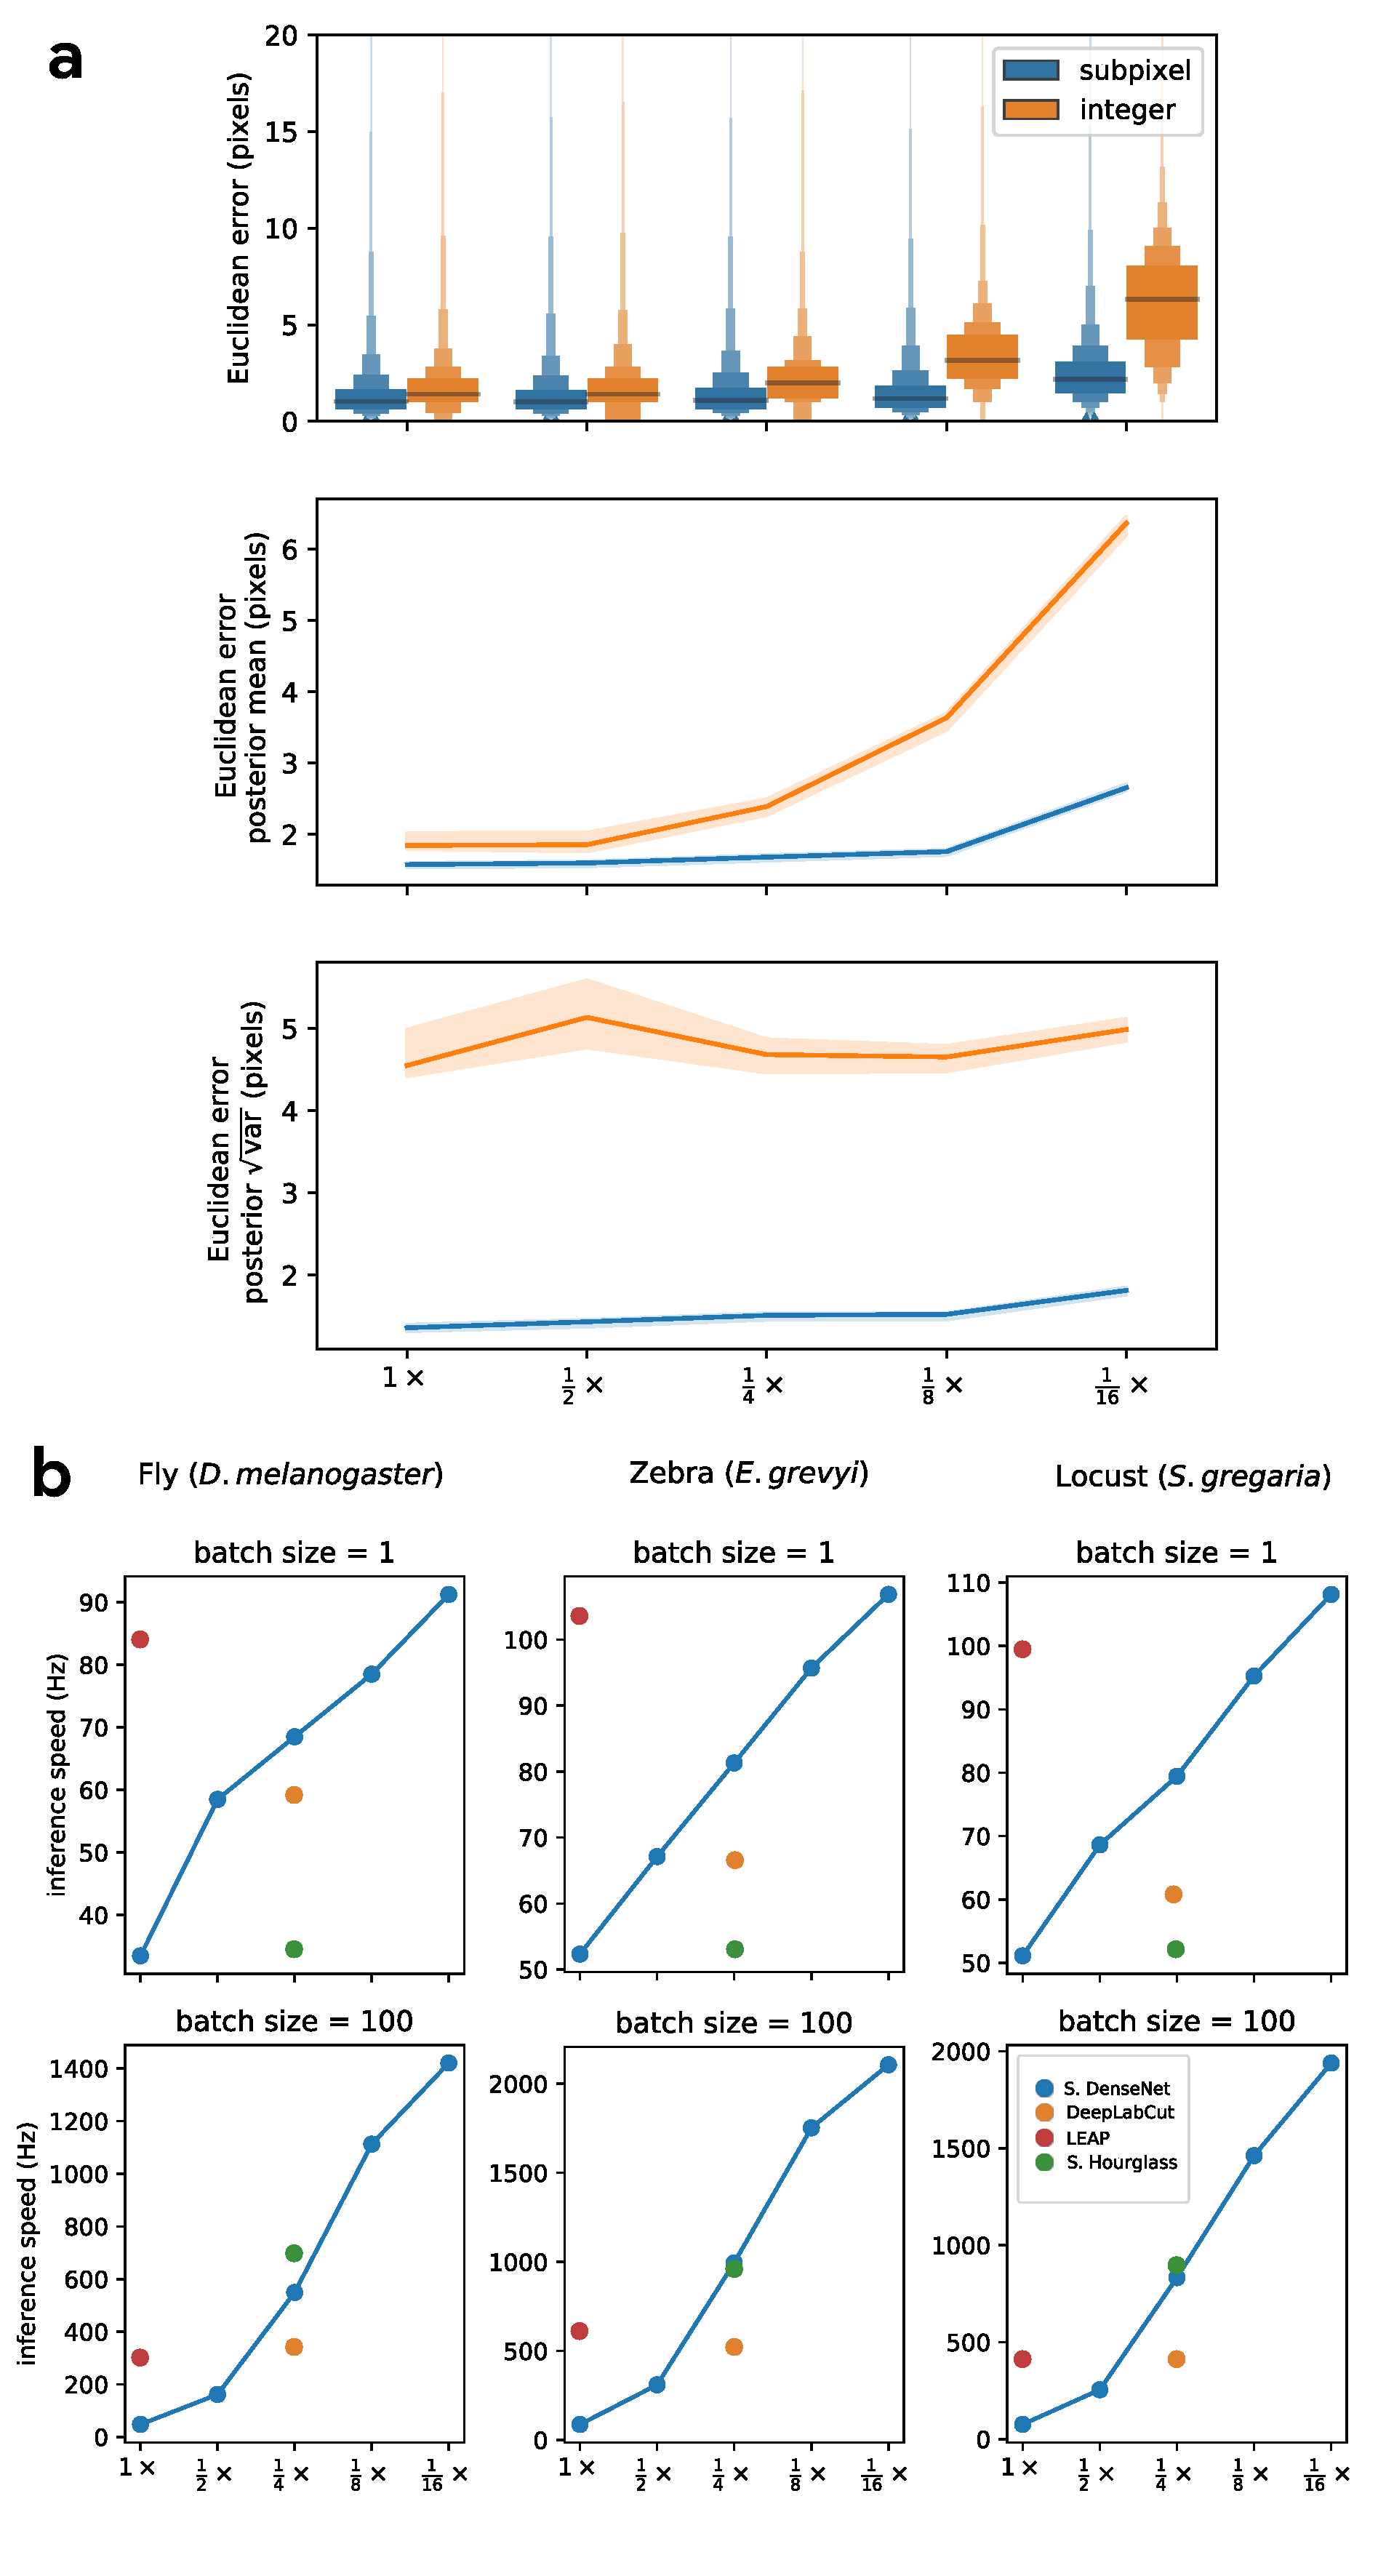
\includegraphics[width=0.60\linewidth]{Graving_IMPRS_Thesis/figures/downsample_inference_speed.pdf}
    \caption{Our subpixel maxima algorithm increases speed without decreasing accuracy. Prediction accuracy on the fly dataset is maintained across downsampling configurations (\textbf{a}). Letter-value plots (\textbf{a-top}) show the raw error distributions for each configuration. Visualizations of the credible intervals (99\% highest-density region) of the posterior distributions for the mean and variance (\textbf{a-bottom}) illustrate statistical differences between the error distributions, where using subpixel maxima decreases both the mean and variance of the error distribution. Inference speed is fast and can be run in real-time on single images (batch size = 1) at $\sim$30-110Hz or offline (batch size = 100) upwards of 1000Hz (\textbf{b}). Plots show the inference speeds for our Stacked DenseNet model across downsampling configurations as well as the other models we tested for each of our datasets. }
    \label{fig:downsample_inference_speed}
    
    
    \end{figure}
    
    \begin{figure}[!htb]
    
    \centering
    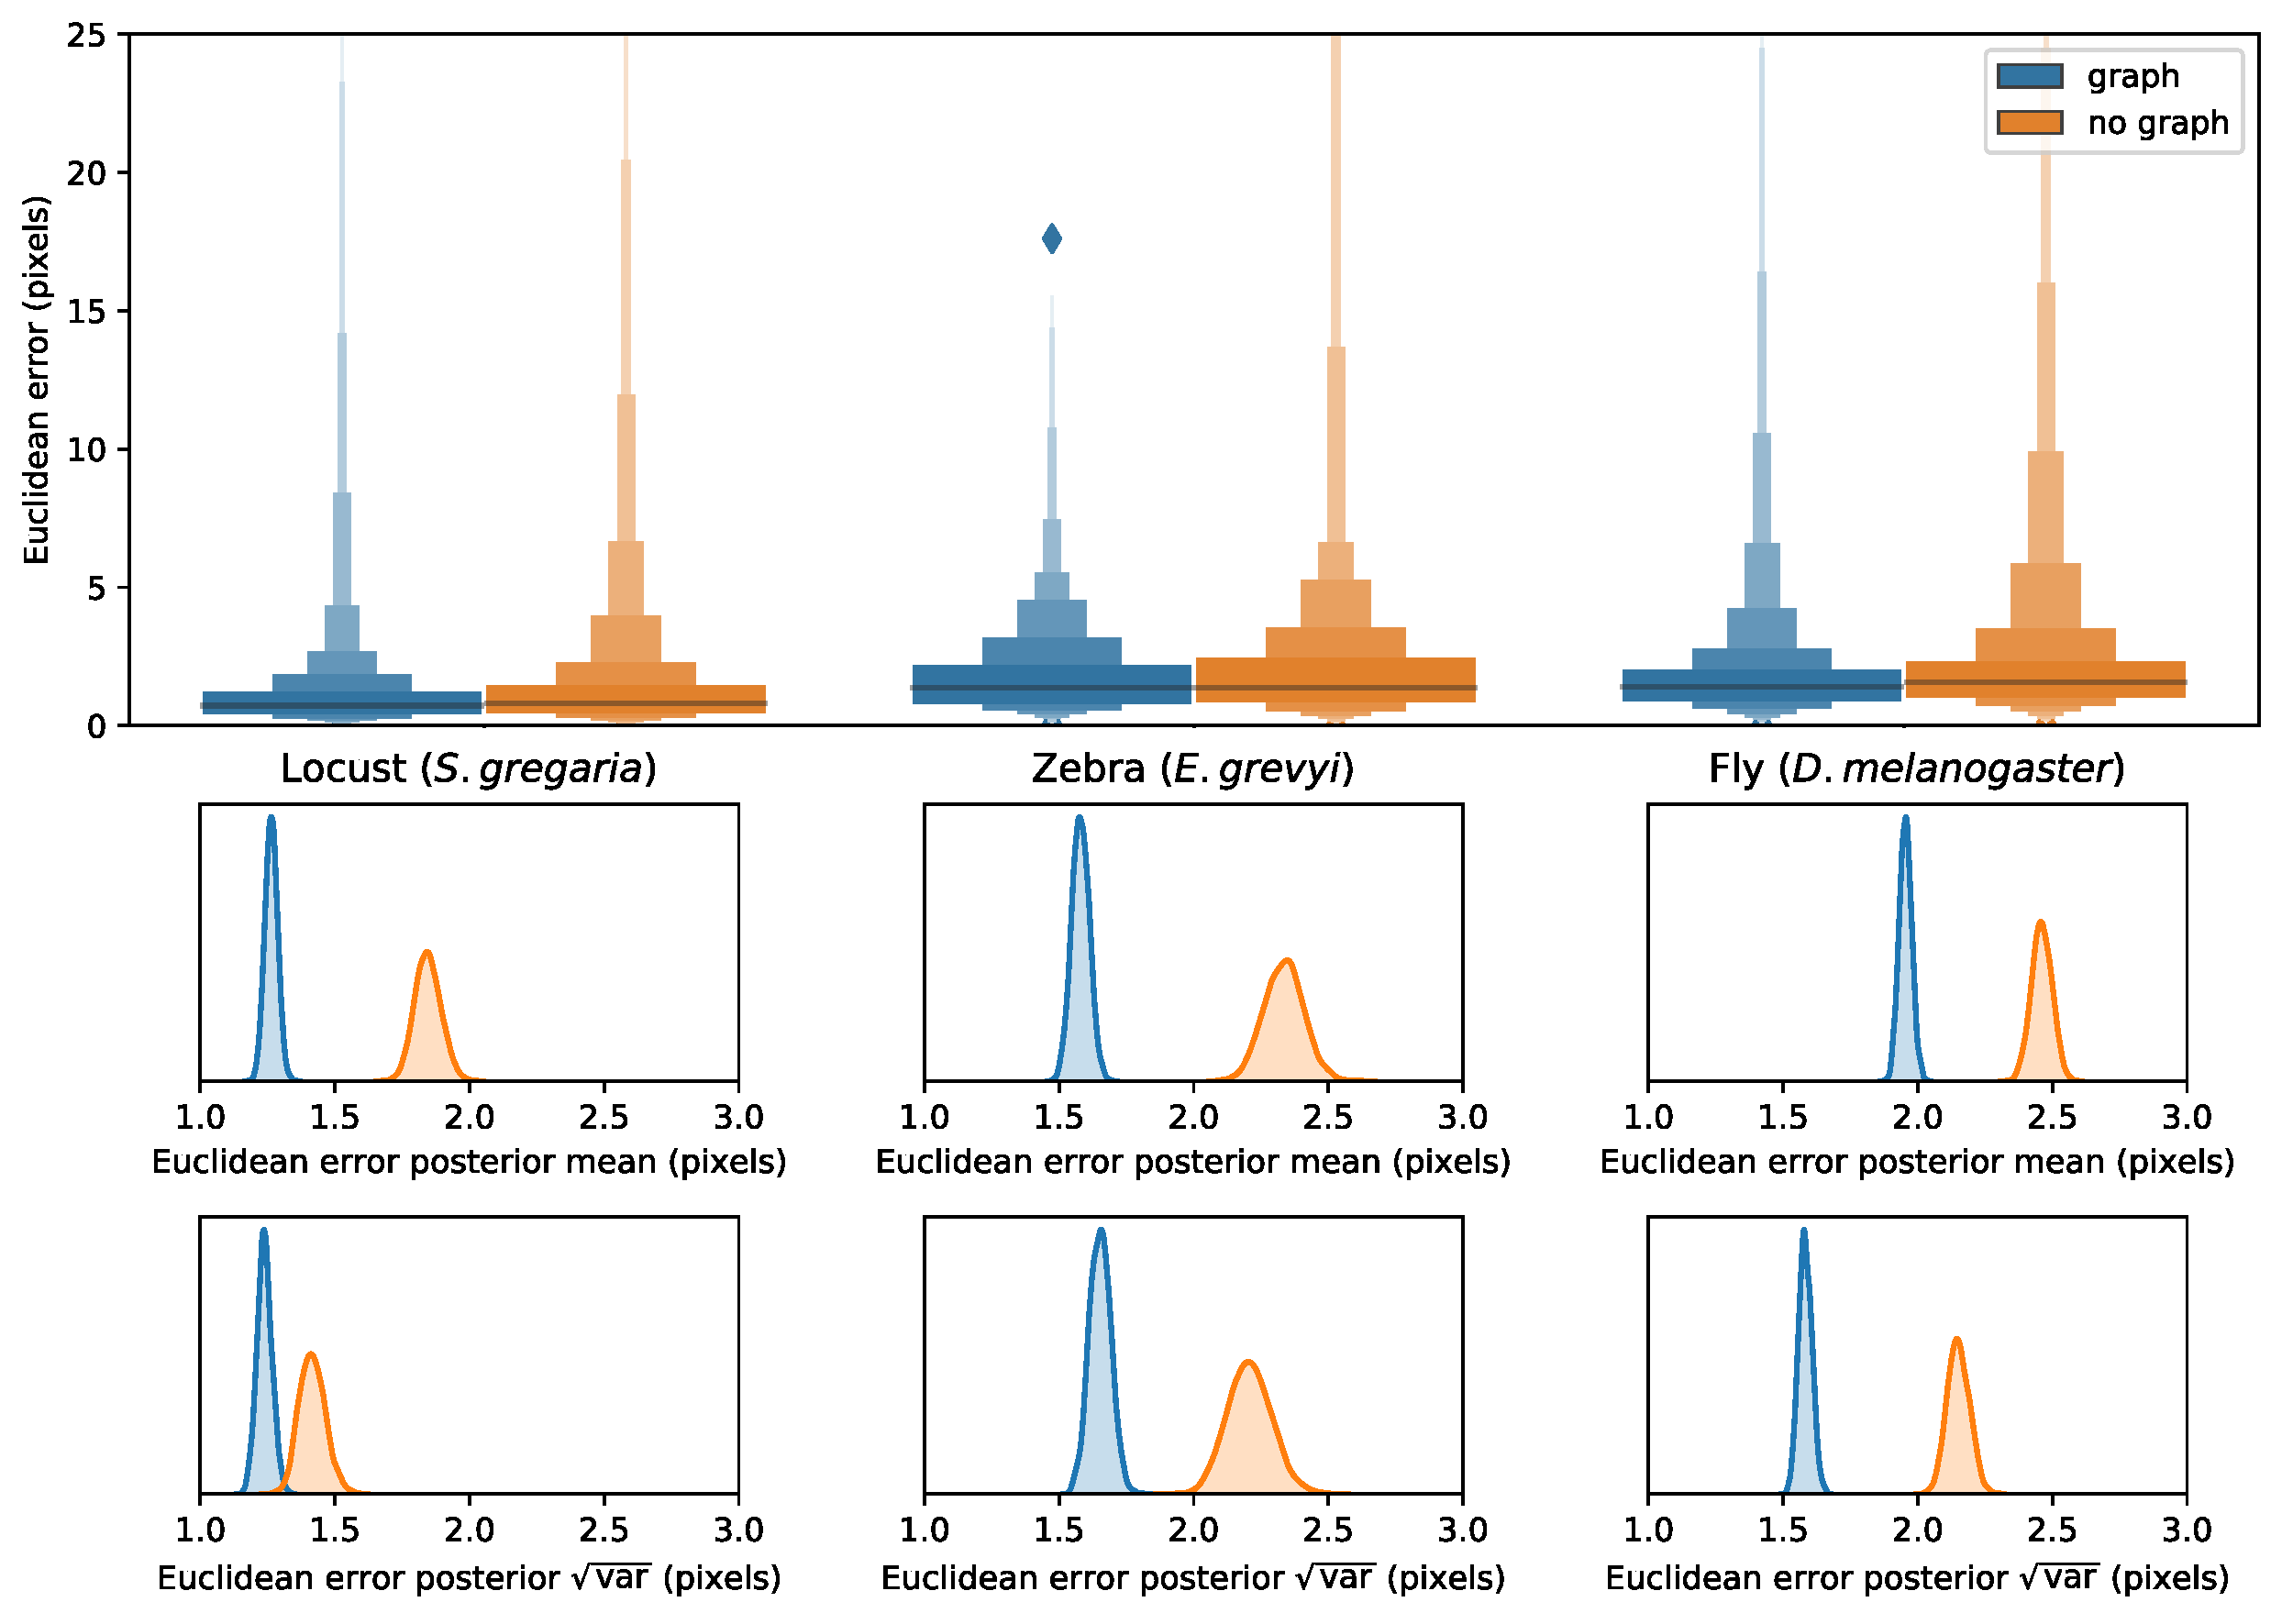
\includegraphics[width=0.76\linewidth]{Graving_IMPRS_Thesis/figures/graph_error_figure.pdf}
    \caption{Predicting the multi-scale geometry of the posture graph reduces error. Letter-value plots (\textbf{top}) show the raw error distributions for each experiment. Visualizations of the posterior distributions for the mean and variance (\textbf{bottom}) show statistical differences between the error distributions. Predicting the posture graph decreases both the mean and variance of the error distribution.}
    \label{fig:graph_error_figure}
    
    
    
    \end{figure}
    
    \begin{figure}[!htb]
    
    \centering
    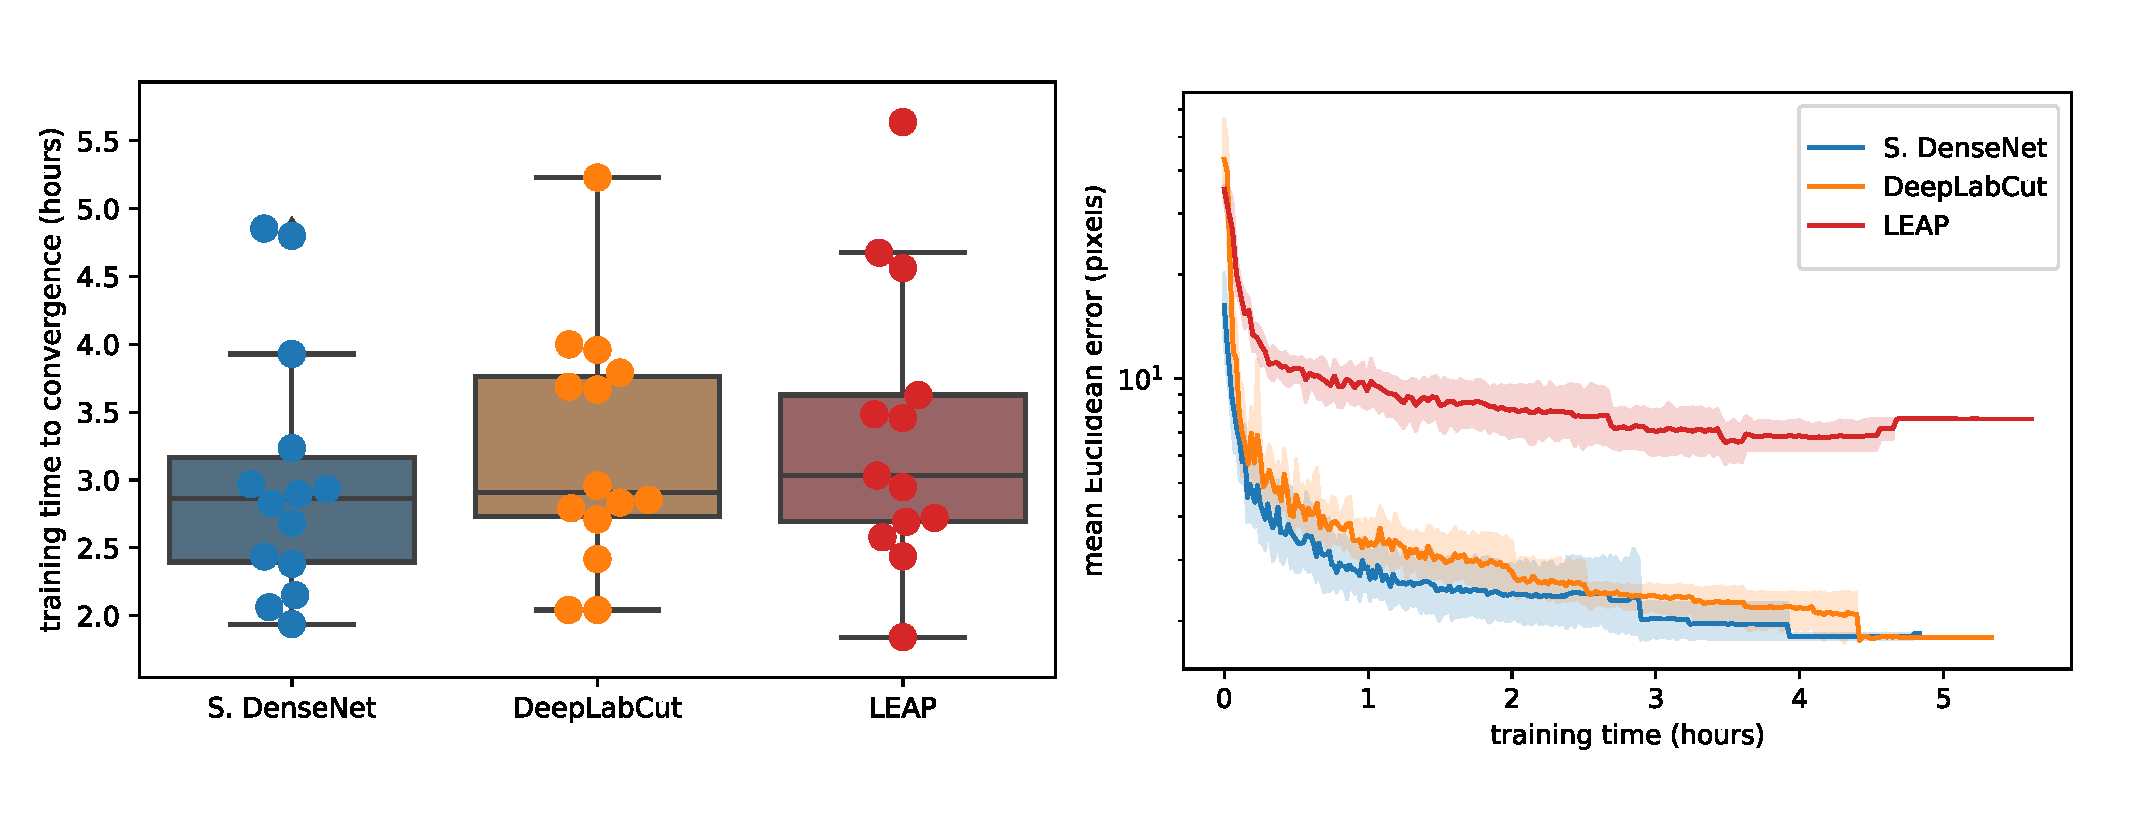
\includegraphics[width=0.8\linewidth]{Graving_IMPRS_Thesis/figures/training_time_figure.pdf}
    \caption{Training time required for our Stacked DenseNet model, the DeepLabCut model \citep{mathis2018deeplabcut}, and the LEAP model \citep{pereira2019fast} (n=15 per model) using our zebra dataset. Boxplots and swarm plots (\textbf{left}) show the total training time to convergence (<0.001 improvement in validation loss for 50 epochs). Line plots (\textbf{right}) illustrate the Euclidean error of the validation set during training, where error bars show bootstrapped (n=1000) 99\% confidence intervals of the mean. Fully training models to convergence requires only a few hours of optimization (\textbf{left}) with reasonable accuracy reached after only 1 hour (\textbf{right}) for our Stacked DenseNet model.}
    \label{fig:training_time}
    
    
    \end{figure}
    
    \begin{figure}[!htb]
    
    \centering
    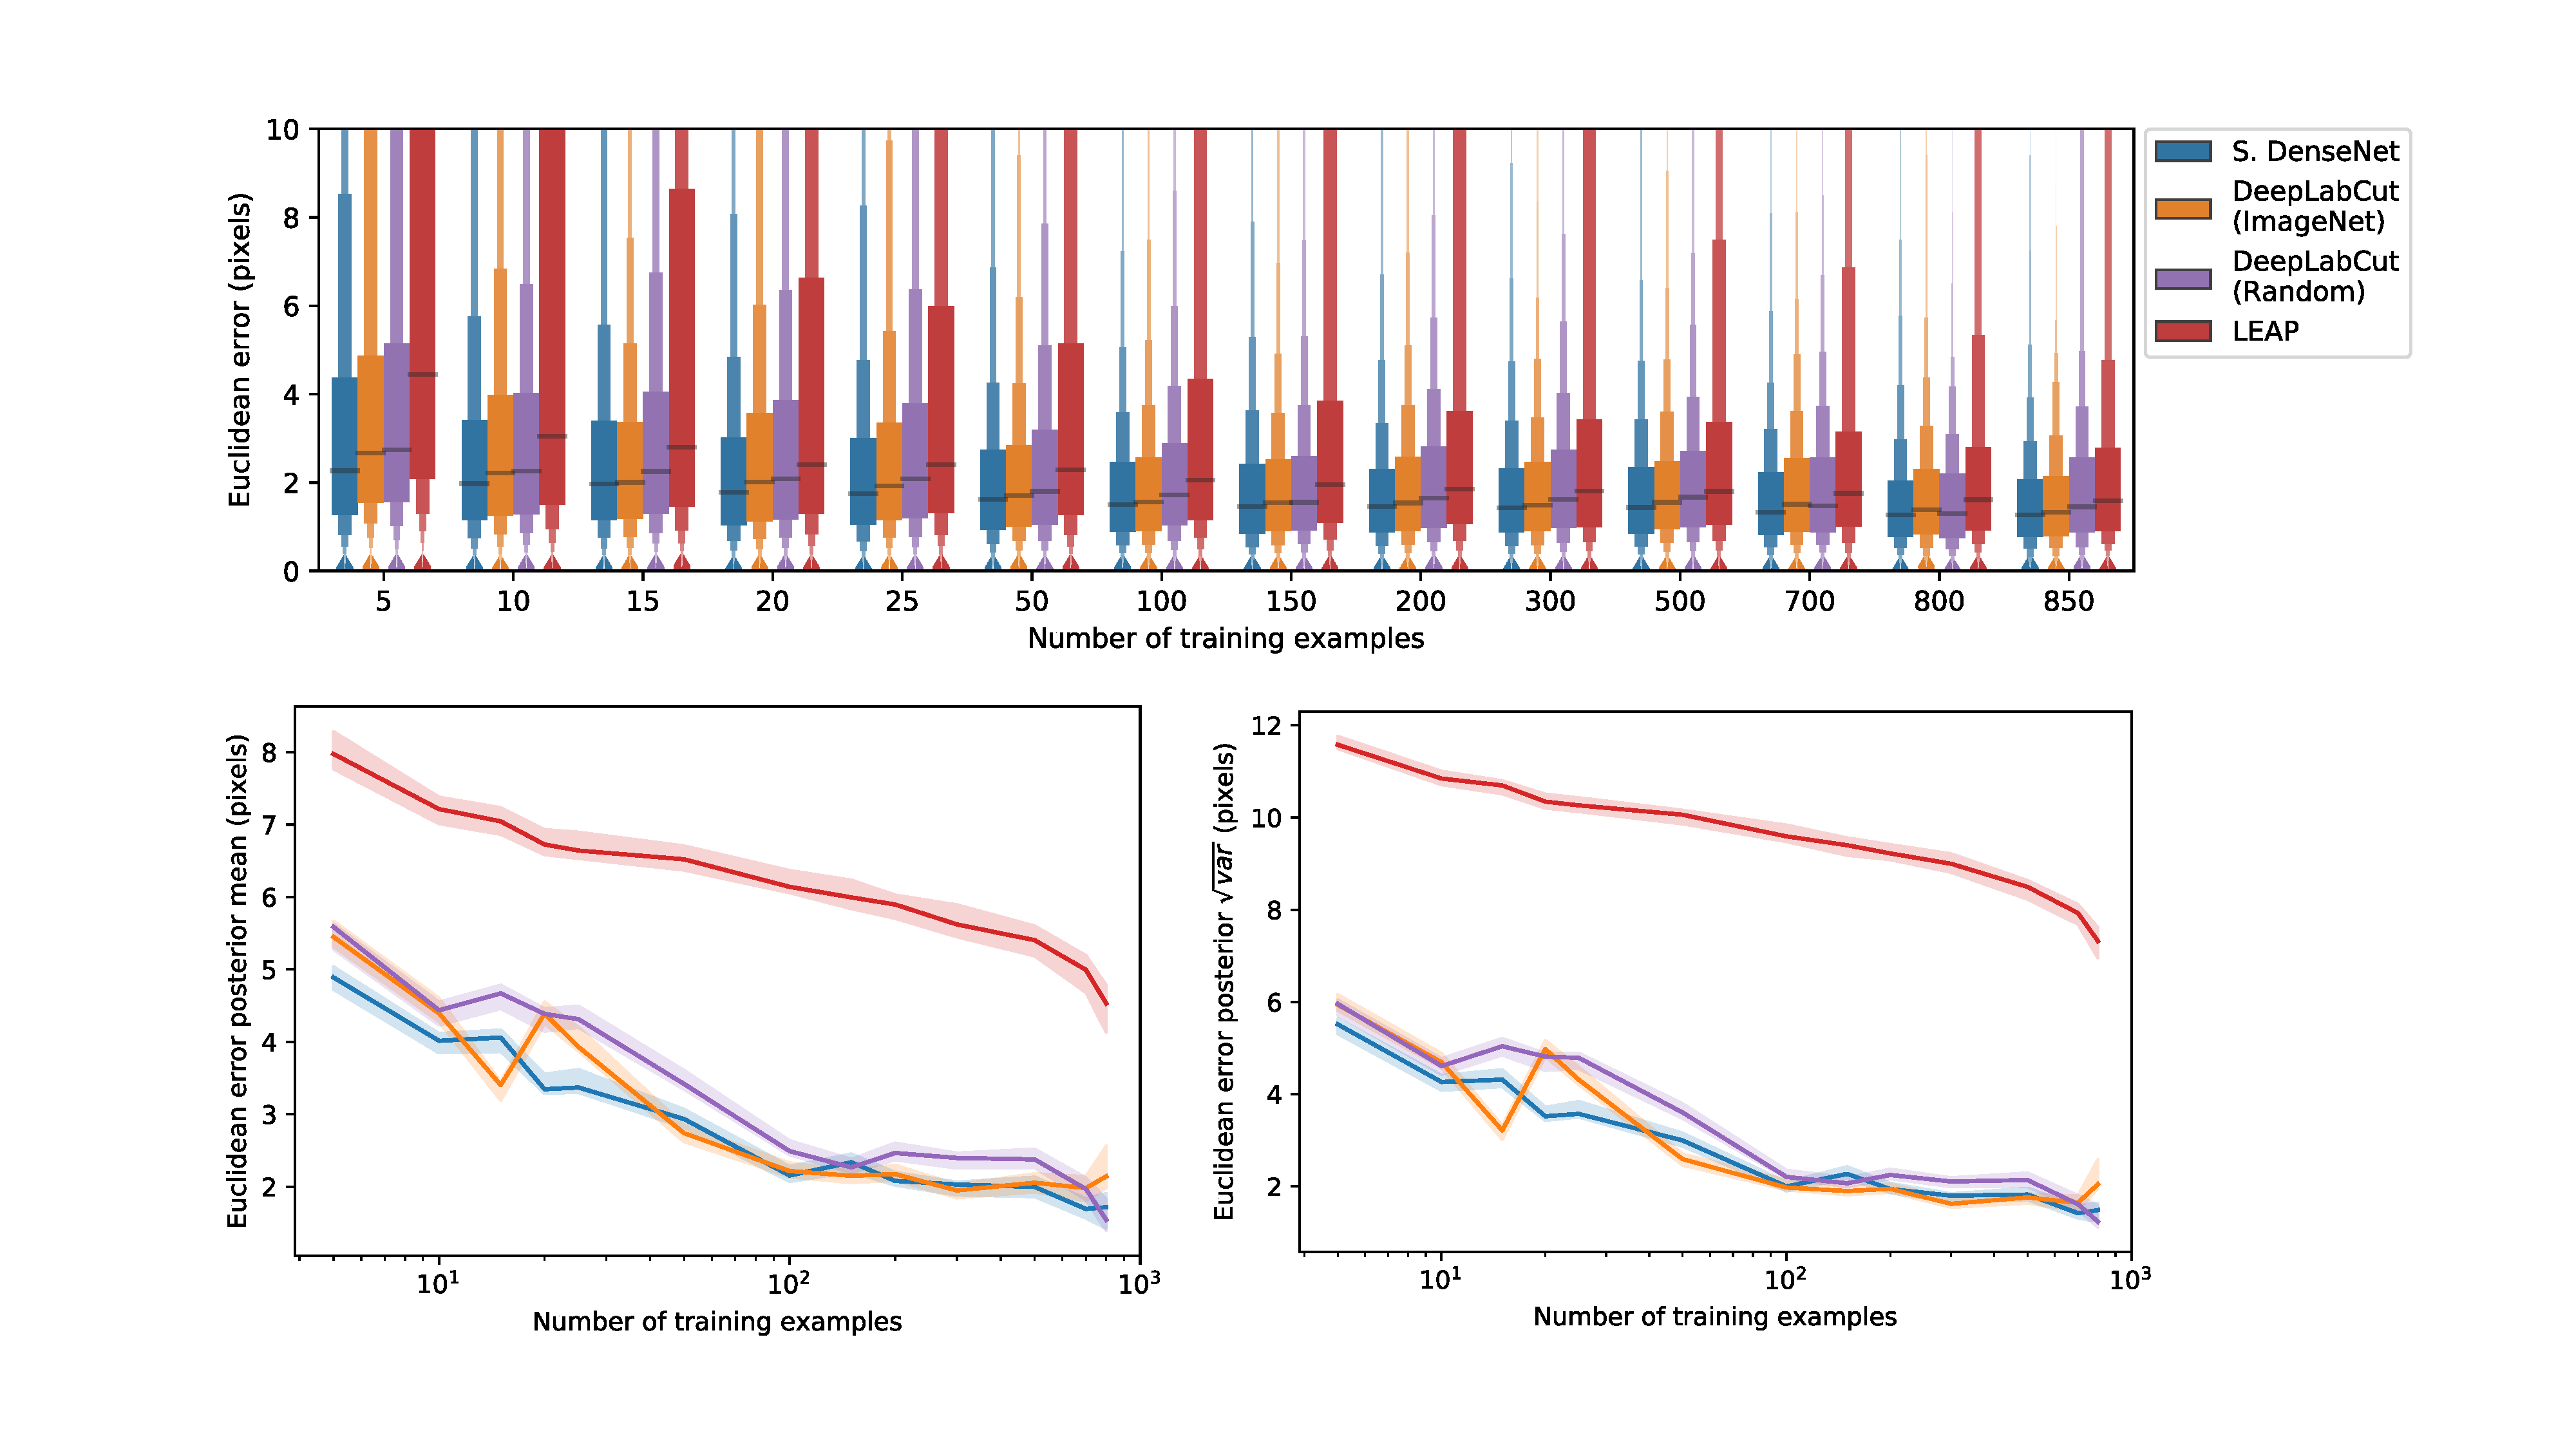
\includegraphics[width=\linewidth]{Graving_IMPRS_Thesis/figures/training_data_proportion_figure.pdf}
    \caption{A comparison of prediction accuracy with different numbers of training examples from our zebra dataset. The error distributions shown as letter-value plots (\textbf{top}) illustrate the Euclidean error for the remainder of the dataset not used for training---with a total of 900 labeled examples in the dataset. Line plots (\textbf{bottom}) show posterior credible intervals (99\% highest-density region) for the mean and variance of the error distributions. We tested our Stacked DenseNet model; the DeepLabCut model \citep{mathis2018deeplabcut} with transfer learning---i.e., with weights pretrained on ImageNet \citep{deng2009imagenet}; the same model without transfer learning---i.e., with randomly-initialized weights; and the LEAP model \citep{pereira2019fast}. Our Stacked DenseNet model achieves high accuracy using few training examples without the use the transfer learning. Using pretrained weights does slightly decrease overall prediction error for the DeepLabCut model \citep{mathis2018deeplabcut}, but the effect size is relatively small.}
    \label{fig:training_prop}
    
    
    \end{figure}
    
    
    
    
    
    %\begin{figure}[!htb]
    %
    %\centering
    %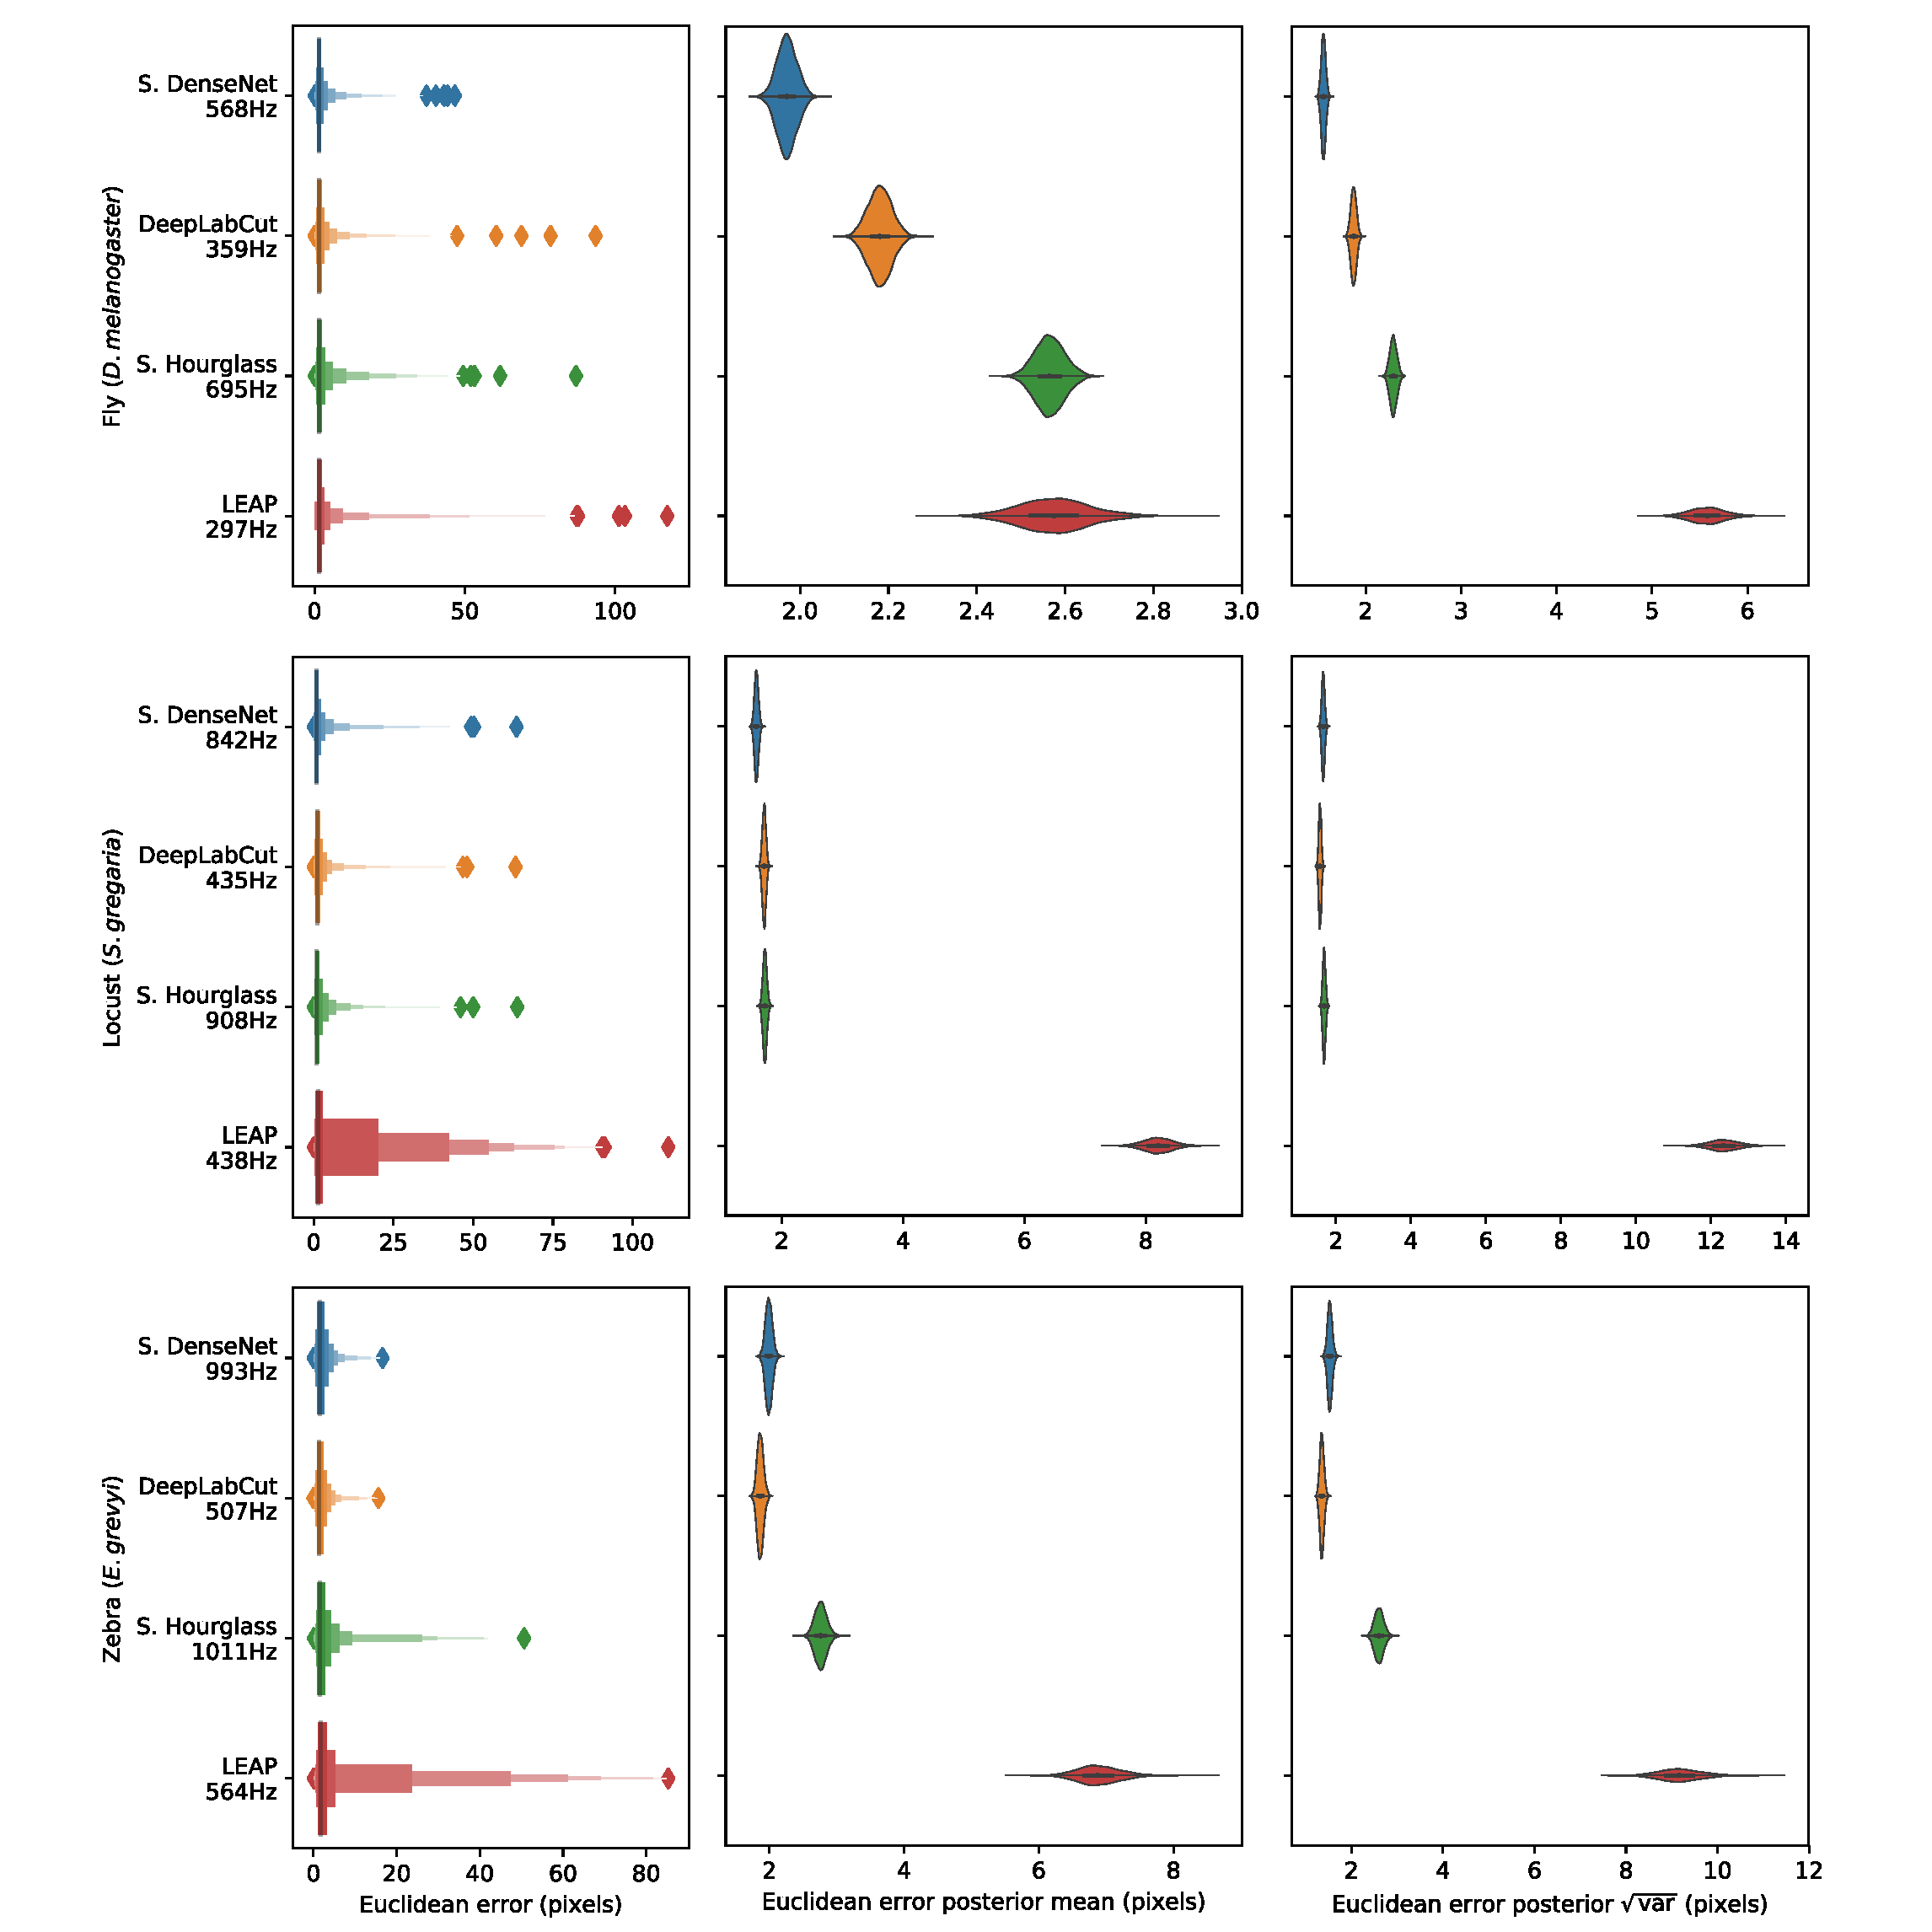
\includegraphics[width=0.75\linewidth]{Graving_IMPRS_Thesis/figures/model_posteriors_figure.pdf}
    %\caption{Euclidean error distributions for each model across our three datasets. Letter-value plots (\textbf{left}) show the raw error distributions for each model. Histograms of the posterior distributions for the mean and variance (\textbf{right}) show statistical differences between the error distributions. Overall the LEAP model \citept{pereira2019fast} was the worst performer on every dataset in terms of both mean and variance. Our implementation of Stacked Densenet was the best performer for the fly dataset, while Stacked DenseNet and DeepLabCut both performed equally well on the locust and zebra datasets. The posteriors for DeepLabCut \citep{mathis2018deeplabcut} and our Stacked DenseNet model are highly overlapping for these datasets, which suggests they are not statistically discernible from one another. The Stacked Hourglass \citep{newell2016} model performed slightly worse than DeepLabCut and our Stacked DenseNet model for all datasets.}
    %\label{fig:model_posteriors_figure}
    %
    %\end{figure}



\section{Convolutional neural networks (CNNs)}
\label{app:cnn}
\textit{Artificial neural networks} like CNNs are complex, non-linear regression models that "learn" a hierarchically–organized set of parameters from real-world data via optimization. These machine learning models are now commonplace in science and industry and have proven to be surprisingly effective for a large number of applications where more conventional statistical models have failed \citep{lecun2015deep}. For computer vision tasks, CNN parameters typically take the form of two-dimensional convolutional filters that are optimized to detect spatial features needed to model relationships between high-dimensional image data and some related variable(s) of interest, such as locations in space—e.g., posture keypoints—or semantic labels \citep{long2015fully,badrinarayanan2017segnet}.

Once a training set is generated (Appendix \ref{app:training_data}), a CNN model must be selected and optimized to perform the prediction task. CNNs are incredibly flexible with regard to how models are specified and trained, which is both an advantage and a disadvantage. This flexibility means models can be adapted to almost any computer vision task, but it also means the number of possible model architectures and optimization schemes is very large. This can make selecting an architecture and specifying hyperparameters a challenging process. However, most research on pose estimation has converged on a set of models that generally work well for this task (Appendix \ref{app:fcnn}).

After selecting an architecture, the parameters of the model are set to an initial value and then iteratively updated to minimize some objective function, or \textit{loss function}, that describes the difference between the model's predictive distribution and the true distribution of the data—in other words, the likelihood of the model's output is maximized. These parameter updates are performed using a modified version of the gradient descent algorithm (\citealt{cauchy1847methode}) known as \textit{mini-batch stochastic gradient descent}—often referred to as simply \textit{stochastic gradient descent} or \textit{SGD} \citep{robbins1951stochastic,kiefer1952stochastic}. SGD iteratively optimizes the model parameters using small randomly-selected subsamples, or \textit{batches}, of training data. Using SGD allows the model to be trained on extremely large datasets in an iterative "online" fashion without the need to load the entire dataset into memory. The model parameters are updated with each batch by adjusting the parameter values in a direction that minimizes the error—where one round of training on the full dataset is commonly referred to as an \textit{epoch}. The original SGD algorithm requires careful selection and tuning of hyperparameters to successfully optimize a model, but modern versions of the algorithm, such as \textit{ADAM} \citep{kingma2014adam}, automatically tune these hyperparameters, which makes optimization more straightforward.

The model parameters are optimized until they reach a convergence criterion, which is some measure of performance that indicates the model has reached a good location in parameter space. The most commonly used convergence criterion is a measure of predictive accuracy—often the loss function used for optimization—on a held-out \textit{validation set}—a subsample of the training data not used for optimization—that evaluates the model's ability to generalize to new "out-of-sample" data. The model is typically evaluated at the end of each training epoch to assess performance on the validation set. Once performance on the validation set stops improving, training is usually stopped to prevent the model from overfitting to the training set—a technique known as \textit{early stopping} \citep{prechelt1998automatic}.



\section{Collecting training data}
\label{app:training_data}

Depending on the variability of the data, CNNs usually require thousands or tens of thousands of manually-annotated examples in order to reach human-level accuracy. However, in laboratory settings, sources of image variation like lighting and spatial scale can be more easily controlled, which minimizes the number of training examples needed to achieve accurate predictions.

This need for a large training set can be further reduced in a number of ways. Two commonly used methods include (1) \textit{transfer learning}—using a model with parameters that are pre-trained on a larger set of images, such as the ImageNet database \citep{deng2009imagenet}, containing diverse features \citep{pratt1993discriminability,insafutdinov2016deepercut, mathis2018deeplabcut}— and (2) \textit{augmentation}— artificially increasing data variance by applying spatial and noise transformations such as flipping (mirroring), rotating, scaling, and adding different forms of noise or artificial occlusions. Both of these methods act as useful forms of \textit{regularization}—incorporating a prior distribution—that allows the model to generalize well to new data even when the training set is small. Transfer learning incorporates prior information that images from the full dataset should contain statistical features similar to other images of the natural world, while augmentation incorporates prior knowledge that animals are bilaterally symmetric, can vary in their body size, position, and orientation, and that noise and occlusions sometimes occur.

\cite{pereira2019fast} introduced two especially clever solutions for collecting an adequate training set. First, they cluster unannotated images based on pixel variance and uniformly sample images from each cluster, which reduces correlation between training examples and ensures the training data are representative of the entire distribution of possible images. Second, they use \textit{active learning} where a CNN is trained on a small number of annotated examples and is then used to initialize keypoint locations for a larger set of unannotated data. These pre-initialized data are then manually corrected by the annotator, the model is retrained, and the unannotated data are re-initialized. The annotator applies this process iteratively as the training set grows larger until they are providing only minor adjustments to the pre-initialized data. This “human-in-the-loop”-style annotation expedites the process of generating an adequately large training set by reducing the cognitive load on the annotator—where the pose estimation model serves as a “cognitive partner”. Such a strategy also allows the annotator to automatically select new training examples based on the performance of the current iteration—where low-confidence predictions indicate examples that should be annotated for maximum improvement (Figure \ref{fig:workflow_figure}).

Of course, annotating image data requires software made for this purpose. \cite{pereira2019fast} provide a custom annotation GUI written in MATLAB specifically designed for annotating posture using an active learning strategy. \cite{mathis2018deeplabcut} recently added a Python-based GUI in an updated version of their software—including active learning and image sampling methods (see \citealt{nath2018}). Our framework also includes a Python-based GUI for annotating data with similar features to \cite{mathis2018deeplabcut} and \cite{pereira2019fast}. 



\section{Fully-convolutional regression}
\label{app:fcnn}

For the task of pose estimation, a CNN is optimized to predict the locations of postural keypoints in an image. One approach is to use a CNN to directly predict the numerical value of each keypoint coordinate as an output. However, making predictions in this way removes real-world constraints on the model's predictive distribution by destroying spatial relationships within images, which negates many of the advantages of using CNNs in the first place.

CNNs are particularly good at transforming one image to produce another related image, or set of images, while preserving spatial relationships and allowing for translation-invariant predictions—a configuration known as a \textit{fully-convolutional neural network} or \textit{F-CNN} \citep{long2015fully}. Therefore, instead of directly regressing images to coordinate values, a popular solution \citep{newell2016, insafutdinov2016deepercut,mathis2018deeplabcut,pereira2019fast} is to optimize a F-CNN that transforms images to predict a stack of output images known as \textit{confidence maps}—one for each keypoint. Each confidence map in the output volume contains a single, two-dimensional, symmetric Gaussian indicating the location of each joint, and the scalar value of the peak indicates the confidence score of the prediction—typically a value between 0 and 1. The confidence maps are then processed to produce the coordinates of each keypoint.

In the case of \textit{multiple pose estimation} where an image contains many individuals, the global geometry of the posture graph is also predicted by training the model to produce \textit{part affinity fields} \citep{cao2017realtime}— directional vector fields drawn between joints in the posture graph—or \textit{pairwise terms} \citep{insafutdinov2016deepercut}—vector fields of the conditional distributions between posture keypoints (e.g., $p(\textrm{foot}|\textrm{head}))$. This allows multiple posture graphs to be disentangled from the image using graph partitioning as the vector fields indicate the probability of the connection between joints (see \citealt{cao2017realtime} for details).


\begin{figure}[!htb]

\begin{center}
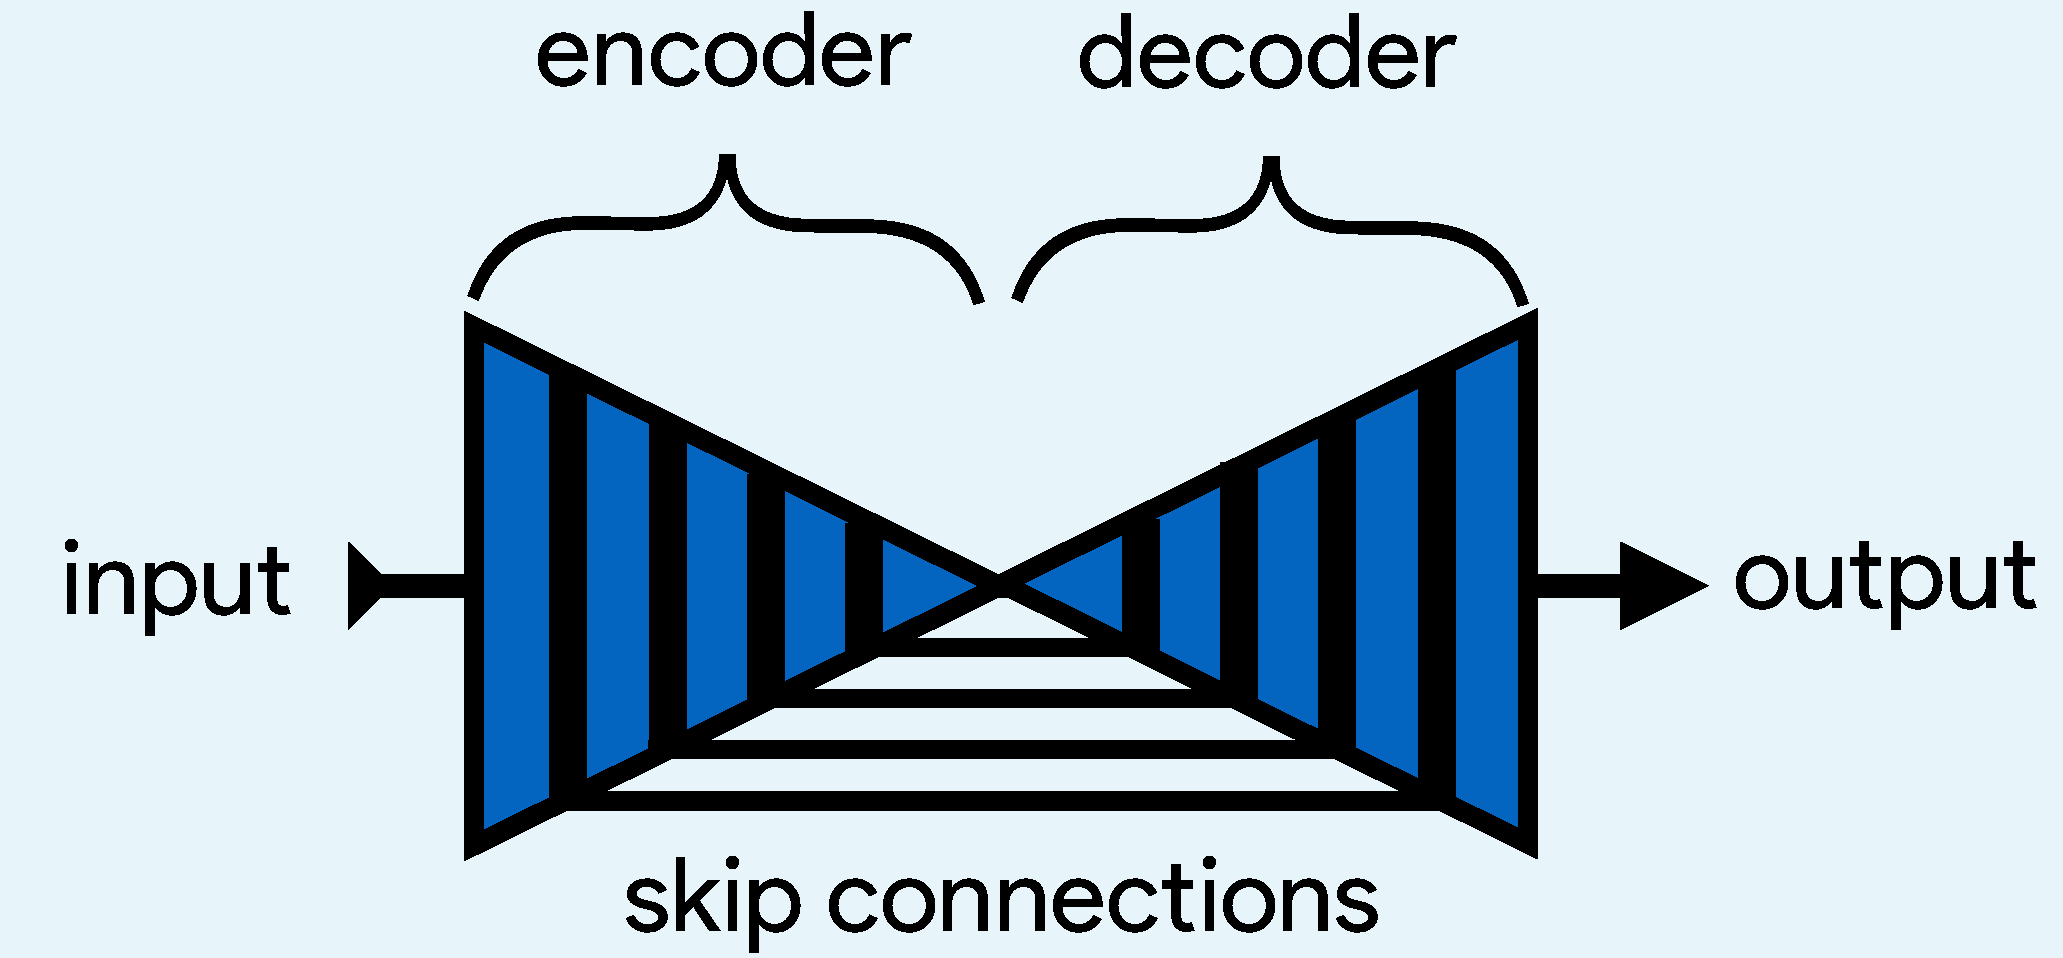
\includegraphics[width=0.5\linewidth]{Graving_IMPRS_Thesis/figures/encoder_decoder_figure.pdf}
\end{center}
\caption{An illustration of the basic encoder-decoder design. The encoder converts the input images into spatial features, and the decoder transforms spatial features to the desired output.}\label{fig:encoder_decoder_figure}
\end{figure}

\section{Encoder-decoder models}
\label{box:encoder_decoder_box}
A popular type of F-CNN (Appendix \ref{app:fcnn}) for solving posture regression problems is known as an \textit{encoder-decoder} model (Figure \ref{fig:encoder_decoder_figure}), which first gained popularity for the task of \textit{semantic segmentation}—a supervised computer vision problem where each pixel in an image is classified into a one of several labeled categories like “dog”, “tree”, or “road” \citep{long2015fully}. This model is designed to repeatedly convolve and downsample input images in the bottom-up \textit{encoder} step and then convolve and upsample the encoder's output in the top-down \textit{decoder} step to produce the final output. Repeatedly applying convolutions and non-linear functions, or \textit{activations}, to the input images transforms pixel values into higher-order spatial features, while downsampling and upsampling respectively increases and decreases the scale and complexity of these features.

\cite{badrinarayanan2017segnet} were the first to popularize a form of this model —known as \textit{SegNet}— for semantic segmentation. However, this basic design is inherently limited because the decoder relies solely on the downsampled output from the encoder, which restricts the features used for predictions to those with the largest spatial scale and highest complexity. For example, a very deep network might learn a complex spatial pattern for predicting “grass” or “trees”, but because it cannot directly access information from the earliest layers of the network, it cannot use the simplest features that plants are green and brown. Subsequent work by \cite{ronneberger2015u} improved on these problems with the addition of \textit{residual} or \textit{skip connections} between the encoder and decoder, where feature maps from encoder layers are concatenated to those decoder layers with the same spatial scale. This set of connections then allows the optimizer, rather than the user, to select the most relevant spatial scale(s) for making predictions.

\cite{Jegou16} are the latest to advance the encoder-decoder paradigm. These researchers introduced a fully-convolutional version of \citeauthor{huang2017densely}’s (\citeyear{huang2017densely}) \textit{DenseNet} architecture known as a \textit{fully-convolutional DenseNet}, or \textit{FC-DenseNet}.  FC-DenseNet’s key improvement is an elaborate set of feed-forward residual connections where the input to each convolutional layer is a concatenated stack of feature maps from all previous layers. This densely-connected design was motivated by the insight that many state-of-the-art models learn a large proportion of redundant features. Most CNNs are not designed so that the final output layers can access all feature maps in the network simultaneously, and this limitation causes these networks to “forget” and “relearn” important features as the input images are transformed to produce the output. In the case of the incredibly popular ResNet-101 \citep{he2016deep} nearly 40\% of the features can be classified as redundant \citep{ayinde2018building}. A densely-connected architecture has the advantages of reduced feature redundancy, increased feature reuse, enhanced feature propagation from early layers to later layers, and subsequently, a substantial reduction in the number of parameters needed to achieve state-of-the-art results \citep{huang2017densely}. Recent work has also shown that DenseNet’s elaborate residual connections have the pleasant side-effect of convexifying the loss landscape during optimization \citep{li2018visualizing}, which allows for faster optimization and increases the likelihood of reaching a good optimum.

\begin{figure}[!htb]

\centering
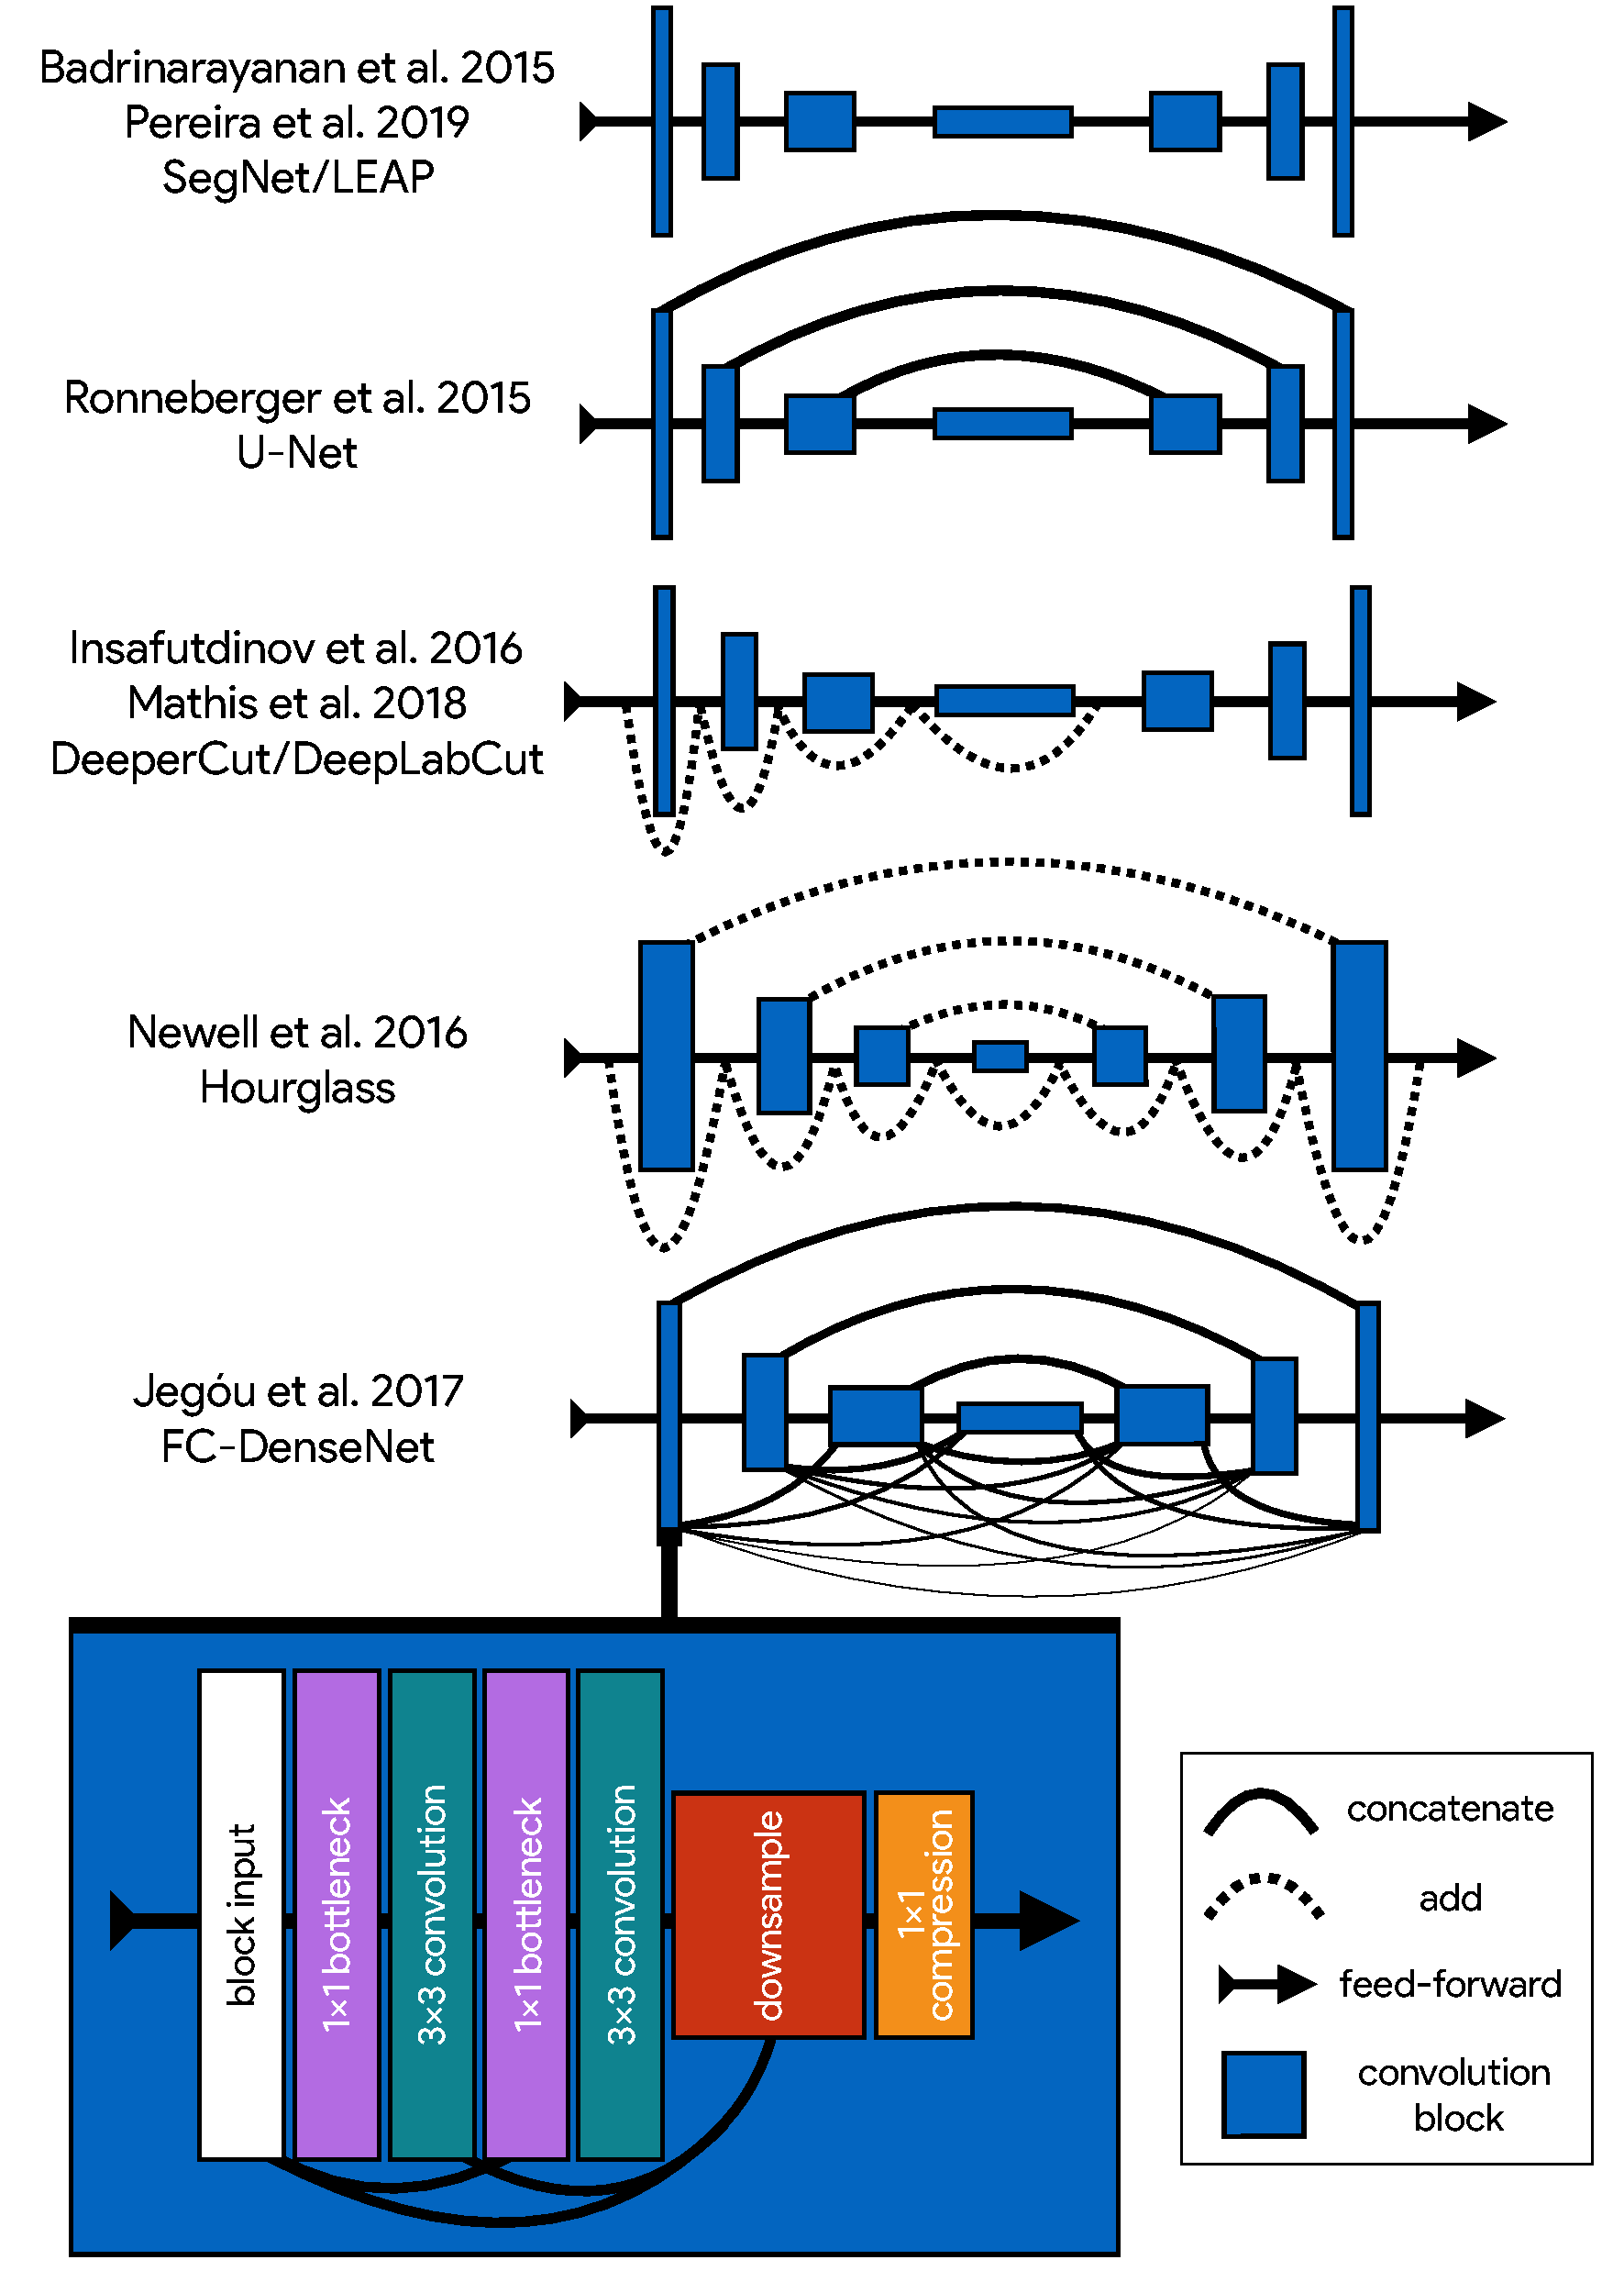
\includegraphics[width=0.75\linewidth]{Graving_IMPRS_Thesis/figures/stacked_densenet_figure.pdf}
\caption{An illustration showing the progression of encoder-decoder architectures from the literature—ordered by performance from top to bottom (see Appendix \ref{app:fcnn} Box \ref{box:encoder_decoder_box} for further details). Most advances in performance have come from adding connections between layers in the network, culminating in FC-DenseNet from \citet{Jegou16}. Lines in each illustration indicate connections between convolutional blocks with the thickness of the line indicating the magnitude of information flow between layers in the network. The size of each convolution block indicates the relative number of feature maps (width) and spatial scale (height). The callout for FC-DenseNet (\citealt{Jegou16}; \textbf{bottom-left}) shows the elaborate set of skip connections within each densely-connected convolutional block as well as our additions of bottleneck and compression layers (described by \citealt{huang2017densely}) to increase efficiency (Appendix \ref{app:implementation})}
\label{fig:stacked_densenet_figure}


\end{figure}

%
%\section{Individual vs. multiple pose estimation}
%\label{app:individual}
%Most recent state-of-the-art methods for posture estimation now focus on simultaneously estimating the pose of multiple individuals in an image (e.g. \citealt{cao2017realtime})—known as \textit{multiple pose estimation}. However, the majority of work on multiple pose estimation has not adequately solved the tracking problem of linking individual data across frames in a video, especially after visual occlusions—although recent work has attempted to address this problem \citep{iqbal2017posetrack, andriluka2018posetrack}. Reliably tracking individuals is important for most behavioral studies, and there are a number of diverse methods already available for solving this problem \citep{perez2014idtracker, crall2015beetag, graving2017pinpoint, romero2018idtracker, wild2018honeybee,boenisch2018tracking}. Additionally, multiple pose estimation requires exhaustively annotating images of multiple individuals—where every individual in the image must be annotated for the model to learn correctly. This type of annotation task is even more laborious and time consuming than annotations for individual pose estimation and increases proportionally with the number of individuals in each frame. Therefore, to avoid solving an already-solved problem of tracking individuals and to circumvent the cognitively complex task of annotating data for multiple pose estimation, the work we describe in this paper is purposefully limited to \textit{individual pose estimation} where each image contains only a single focal individual—which may be localized and cropped from a larger multi-individual image.

%We created a top-down posture estimation framework that can be easily adapted to any data collection workflow, which could include any method for localizing and tracking individuals. This extra step of localizing and tracking individuals, of course, increases the processing time for going from raw images to posture data, which varies depending on the algorithm being used and the number of individuals in each frame. However, increased processing time using automated algorithms is a reasonable trade-off given the alternative of increased manual labor when annotating data—especially considering that the data from most multiple pose estimation algorithms still needs to be linked for each individual across frames to maintain identity. Limiting our methods in this way also simplifies the pose detection problem for designing pose estimation models, which allows for the use of our fast subpixel maxima algorithm on the GPU—as local peak detection is not required. Additionally, because individual pose estimation is such a well-studied problem in computer vision, we can build on the state-of-the-art for this task (see Appendices \ref{app:fcnn} and \ref{app:sota} for details).
%


\label{app:sota}
\section{The state of the art for individual pose estimation}
Many of the current state-of-the-art models for individual posture estimation are based on the design from \cite{newell2016} (e.g., \citealt{Ke_2018_ECCV}, 
\citealt{chen2017adversarial}; also see benchmark results from \citealt{andriluka14cvpr}), but employ various modifications that increase complexity to improve performance. \cite{newell2016} employ what they call a \textit{Stacked Hourglass} network (Appendix \ref{app:fcnn} Figure \ref{fig:stacked_densenet_figure}), which consists of a series of multi-scale encoder-decoder \textit{hourglass} modules connected together in a feed-forward configuration (Figure \ref{fig:model_training_figure}). The main novelties these researchers introduce include (1) stacking multiple hourglass networks together for repeated top-down-bottom-up inference, (2) using convolutional blocks based on the ResNet architecture \citep{he2016deep} with residual connections between the input and output of each block, and (3) using residual connections between the encoder and decoder (similar to \citealt{ronneberger2015u}) with residual blocks in between. \cite{newell2016} also apply a technique known as \textit{intermediate supervision} (Figure \ref{fig:model_training_figure}) where the loss function used for model training is applied to the output of each hourglass as a way of improving optimization across the model's many layers. Recent work by \cite{Jegou16} has further improved on this encoder-decoder design (see Appendix \ref{app:fcnn} Box \ref{box:encoder_decoder_box} and Appendix \ref{app:fcnn} Figure \ref{fig:stacked_densenet_figure}), but to the best of our knowledge, the model introduced by \cite{Jegou16} has not been previously applied to pose estimation.



\label{app:overparam}
\section{Overparameterization and the limitations of LEAP}
Overparameterization is a key limitation for many pose estimation methods, and addressing this problem is critical for high-performance applications. \cite{pereira2019fast} approached this problem by designing their LEAP model after the model from \cite{badrinarayanan2017segnet}, which is a straighforward encoder-decoder design (Appendix \ref{app:fcnn}  Figure \ref{fig:stacked_densenet_figure}; Appendix \ref{app:fcnn} Box \ref{box:encoder_decoder_box}). They benchmarked their model on posture estimation tasks for laboratory animals and compared performance with the more-complex Stacked Hourglass model from \cite{newell2016}. They found their smaller, simplified model achieved equal or better median accuracy with dramatic improvements in inference speed up to 185 Hz. However, \cite{pereira2019fast} first rotationally and translationally aligned each image to improve performance, and their reported inference speeds do not include this computationally expensive preprocessing step. Additionally, rotationally and translationally aligning images is not always possible when the background is complex or highly-variable—such as in field settings—or the study animal has a non-rigid body. This limitation makes the LEAP model \citep{pereira2019fast} unsuitable in many cases. While their approach is simple and effective for a multitude of experimental setups, the LEAP model \citep{pereira2019fast} is also implicitly limited in the same ways as \citeauthor{badrinarayanan2017segnet}’s SegNet model (see Appendix \ref{app:fcnn} Box \ref{box:encoder_decoder_box} for details). The LEAP model cannot make predictions using multiple spatial scales and is not robust to data variance such as rotations \citep{pereira2019fast}.





\label{app:bayesian}
\section{Linear model fitting with Stan}
We estimated the joint posterior $p(\theta_{\mu},\theta_{\phi}|X,y)$ for each model using the No-U-Turn Sampler (NUTS; \citealt{hoffman2014nuts}), a self-tuning variant of the Hamiltonian Monte Carlo (HMC) algorithm \citep{duane1987hybrid}, implemented in Stan \citep{Carpenter_stan:a}. We drew HMC samples using 4 independent Markov chains consisting of 1,000 warm-up iterations and 1,000 sampling iterations for a total of 4,000 sampling iterations. To speed up sampling, we randomly subsampled 20$\%$ of the data from each replicate when fitting each linear model, and we fit each model 5 times to ensure the results were consistent. All models converged without any signs of pathological behavior. We performed a posterior predictive check by visually inspecting predictive samples to assess model fit. For our priors we chose relatively uninformative distributions $\theta_{\mu} \sim \mathit{Cauchy}(0, 5)$ and $\theta_{\phi} \sim \mathit{Cauchy}(0, 10)$, but we found that the choice of prior generally did not have an effect on the final result due to the large amount of data used to fit each model.



\label{app:implementation}

\section{Stacked DenseNet}
Our Stacked DenseNet model consists of an initial 7$\times$7 convolutional layer with stride 2, to efficiently downsample the input resolution—following \cite{newell2016}—followed by a stack of densely-connected hourglass networks with intermediate supervision (Appendix \ref{app:sota}) applied at the output of each network. We also include hyperparameters for the bottleneck and compression layers described by \cite{huang2017densely} to make the model as efficient as possible. These consist of applying a 1$\times$1 convolution to inexpensively compress the number of feature maps before each 3$\times$3 convolution as well as when downsampling and upsampling (see \citealt{huang2017densely} and Appendix \ref{app:fcnn} Figure \ref{fig:stacked_densenet_figure} for details).

\section{Model hyperparameters}
For our Stacked Hourglass model we used a block size of 64 filters (64 filters per 3$\times$3 convolution) with a bottleneck factor of 2 (64/2 = 32 filters per 1$\times$1 bottleneck block). For our Stacked DenseNet model we used a growth rate of 48 (48 filters per 3$\times$3 convolution), a bottleneck factor of 1 (1$\times$growth rate = 48 filters per 1$\times$1 bottleneck block), and a compression factor of 0.5 (feature maps compressed with 1$\times$1 convolution to 0.5$m$ when upsampling and downsampling, where $m$ is the number of feature maps). For our Stacked DenseNet model we also replaced the typical configuration of batch normalization and ReLU activations \citep{goodfellow2016deep} with the more recently-developed self-normalizing SELU activation function \citep{klambauer2017self}, as we found this modification increased inference speed. For the LEAP model \citep{pereira2019fast} we used a 1$\times$ resolution output with integer-based global maxima because we wanted to compare our more complex models with this model in the original configuration described by \citet{pereira2019fast}. The LEAP model could be modified to output smaller confidence maps and increase inference speed, but because there is no obvious "best" way to alter the model to achieve this, we forgo any modification. Additionally, applying our subpixel maxima algorithm at high resolution reduces inference speed compared to integer-based maxima, so this would bias our speed comparisons. 

\section{Our implementation of the DeepLabCut model}
Because the DeepLabCut model from \cite{mathis2018deeplabcut} was not implemented in Keras (a requirement for our pose estimation framework), we re-implemented it. Implementing this model directly in our framework is important to ensure model training and data augmentation are identical when making comparisons between models.  As a consequence, our version of this model does not exactly match the description in the paper but is identical except for the output. Rather than using the location refinement maps described by \cite{insafutdinov2016deepercut} and post-processing confidence maps on the CPU, our version of the DeepLabCut model \citep{mathis2018deeplabcut} has an additional transposed convolutional layer to upsample the output to $\frac{1}{4}\times$ resolution and uses our subpixel maxima algorithm.

To demonstrate that our implementation of the DeepLabCut model matches the performance described by \cite{mathis2018deeplabcut}, we compared prediction accuracy between the two frameworks using the odor-trail mouse dataset provided by \cite{mathis2018deeplabcut} (downloaded from \url{https://github.com/AlexEMG/DeepLabCut/}). This dataset consists of 116 images of a freely-moving individual mouse labeled with four keypoints describing the location of the snout, ears, and the base of the tail. See \cite{mathis2018deeplabcut} for further details on this dataset. We trained both models using 95\% training and 5\% validation data and applied data augmentations for both frameworks using the data augmentation procedure described by \cite{nath2018}. We tried to match these data augmentations as best as possible in DeepPoseKit; however, rather than cropping images as described by \cite{nath2018}, we randomly translated the images independently along the horizontal and vertical axis by drawing from a uniform distribution in the range [-100\%, +100\%]---where percentages are relative to the size of each axis. Translating the images in this way should serve the same purpose as cropping them. 

We trained the original DeepLabCut model \citep{mathis2018deeplabcut} using the default settings and recommendations from \cite{nath2018} for 1 million training iterations. See \cite{mathis2018deeplabcut, nath2018} for further details on the data augmentation and training routine for the original implementation of the DeepLabCut model \citep{mathis2018deeplabcut}. For our re-implementation of the DeepLabCut model \citep{mathis2018deeplabcut} we trained the model with the same batch size and optimization scheme described in the "Model training" section. We then calculated the the prediction accuracy on the full data set. We repeated this procedure five times for each model and fit a Bayesian linear model to a randomly selected subset of the evaluation data to compare the results statistically (see Appendix \ref{app:bayesian}). 

These results demonstrate that our re-implementation of and modification to the DeepLabCut model \citep{mathis2018deeplabcut} have little effect on prediction accuracy (Appendix \ref{app:implementation} Figure \ref{fig:dlc_comparison}). We also provide qualitative comparisons of these results in Appendix \ref{app:implementation} Figure \ref{fig:dlc_comparison}-Figure supplement \ref{figsupp:dlc_tsplot} and Appendix \ref{app:implementation} Figure \ref{fig:dlc_comparison}-video \ref{videosupp:dlcsv1}. For these qualitative comparisons, we also added an additional rotational augmentation (drawing from a uniform distribution in the range [-180$\degree$, +180$\degree$)) when training our implementation of the DeepLabCut model \citep{mathis2018deeplabcut} as we noticed this improved generalization to the video for situations where the mouse rotated its body axis. To the best of our knowledge, rotational augmentations are not currently available when using the software from \cite{mathis2018deeplabcut, nath2018}, which demonstrates the flexibility of the data augmentation pipeline \citep{jung2018imgaug} for DeepPoseKit. The inference speed for the odor-trail mouse dataset using our implementation of the DeepLabCut model \citep{mathis2018deeplabcut} is $\sim$49Hz with a batch size of 64 (offline speeds) and $\sim$35Hz with a batch size of 1 (real-time speeds) at full resolution 640$\times$480, which matches well with results from \cite{mathis2018inference} of $\sim$47Hz and $\sim$32Hz respectively. This suggests our modifications did not affect the speed of the model and that our speed comparisons are also reasonable. Because the training routine could be changed for any underlying model---including the new models we present in this paper---this factor is not relevant when making comparisons as long as training is identical for all models being compared, which we ensure when performing our comparisons.

 
\begin{figure}[!htb]
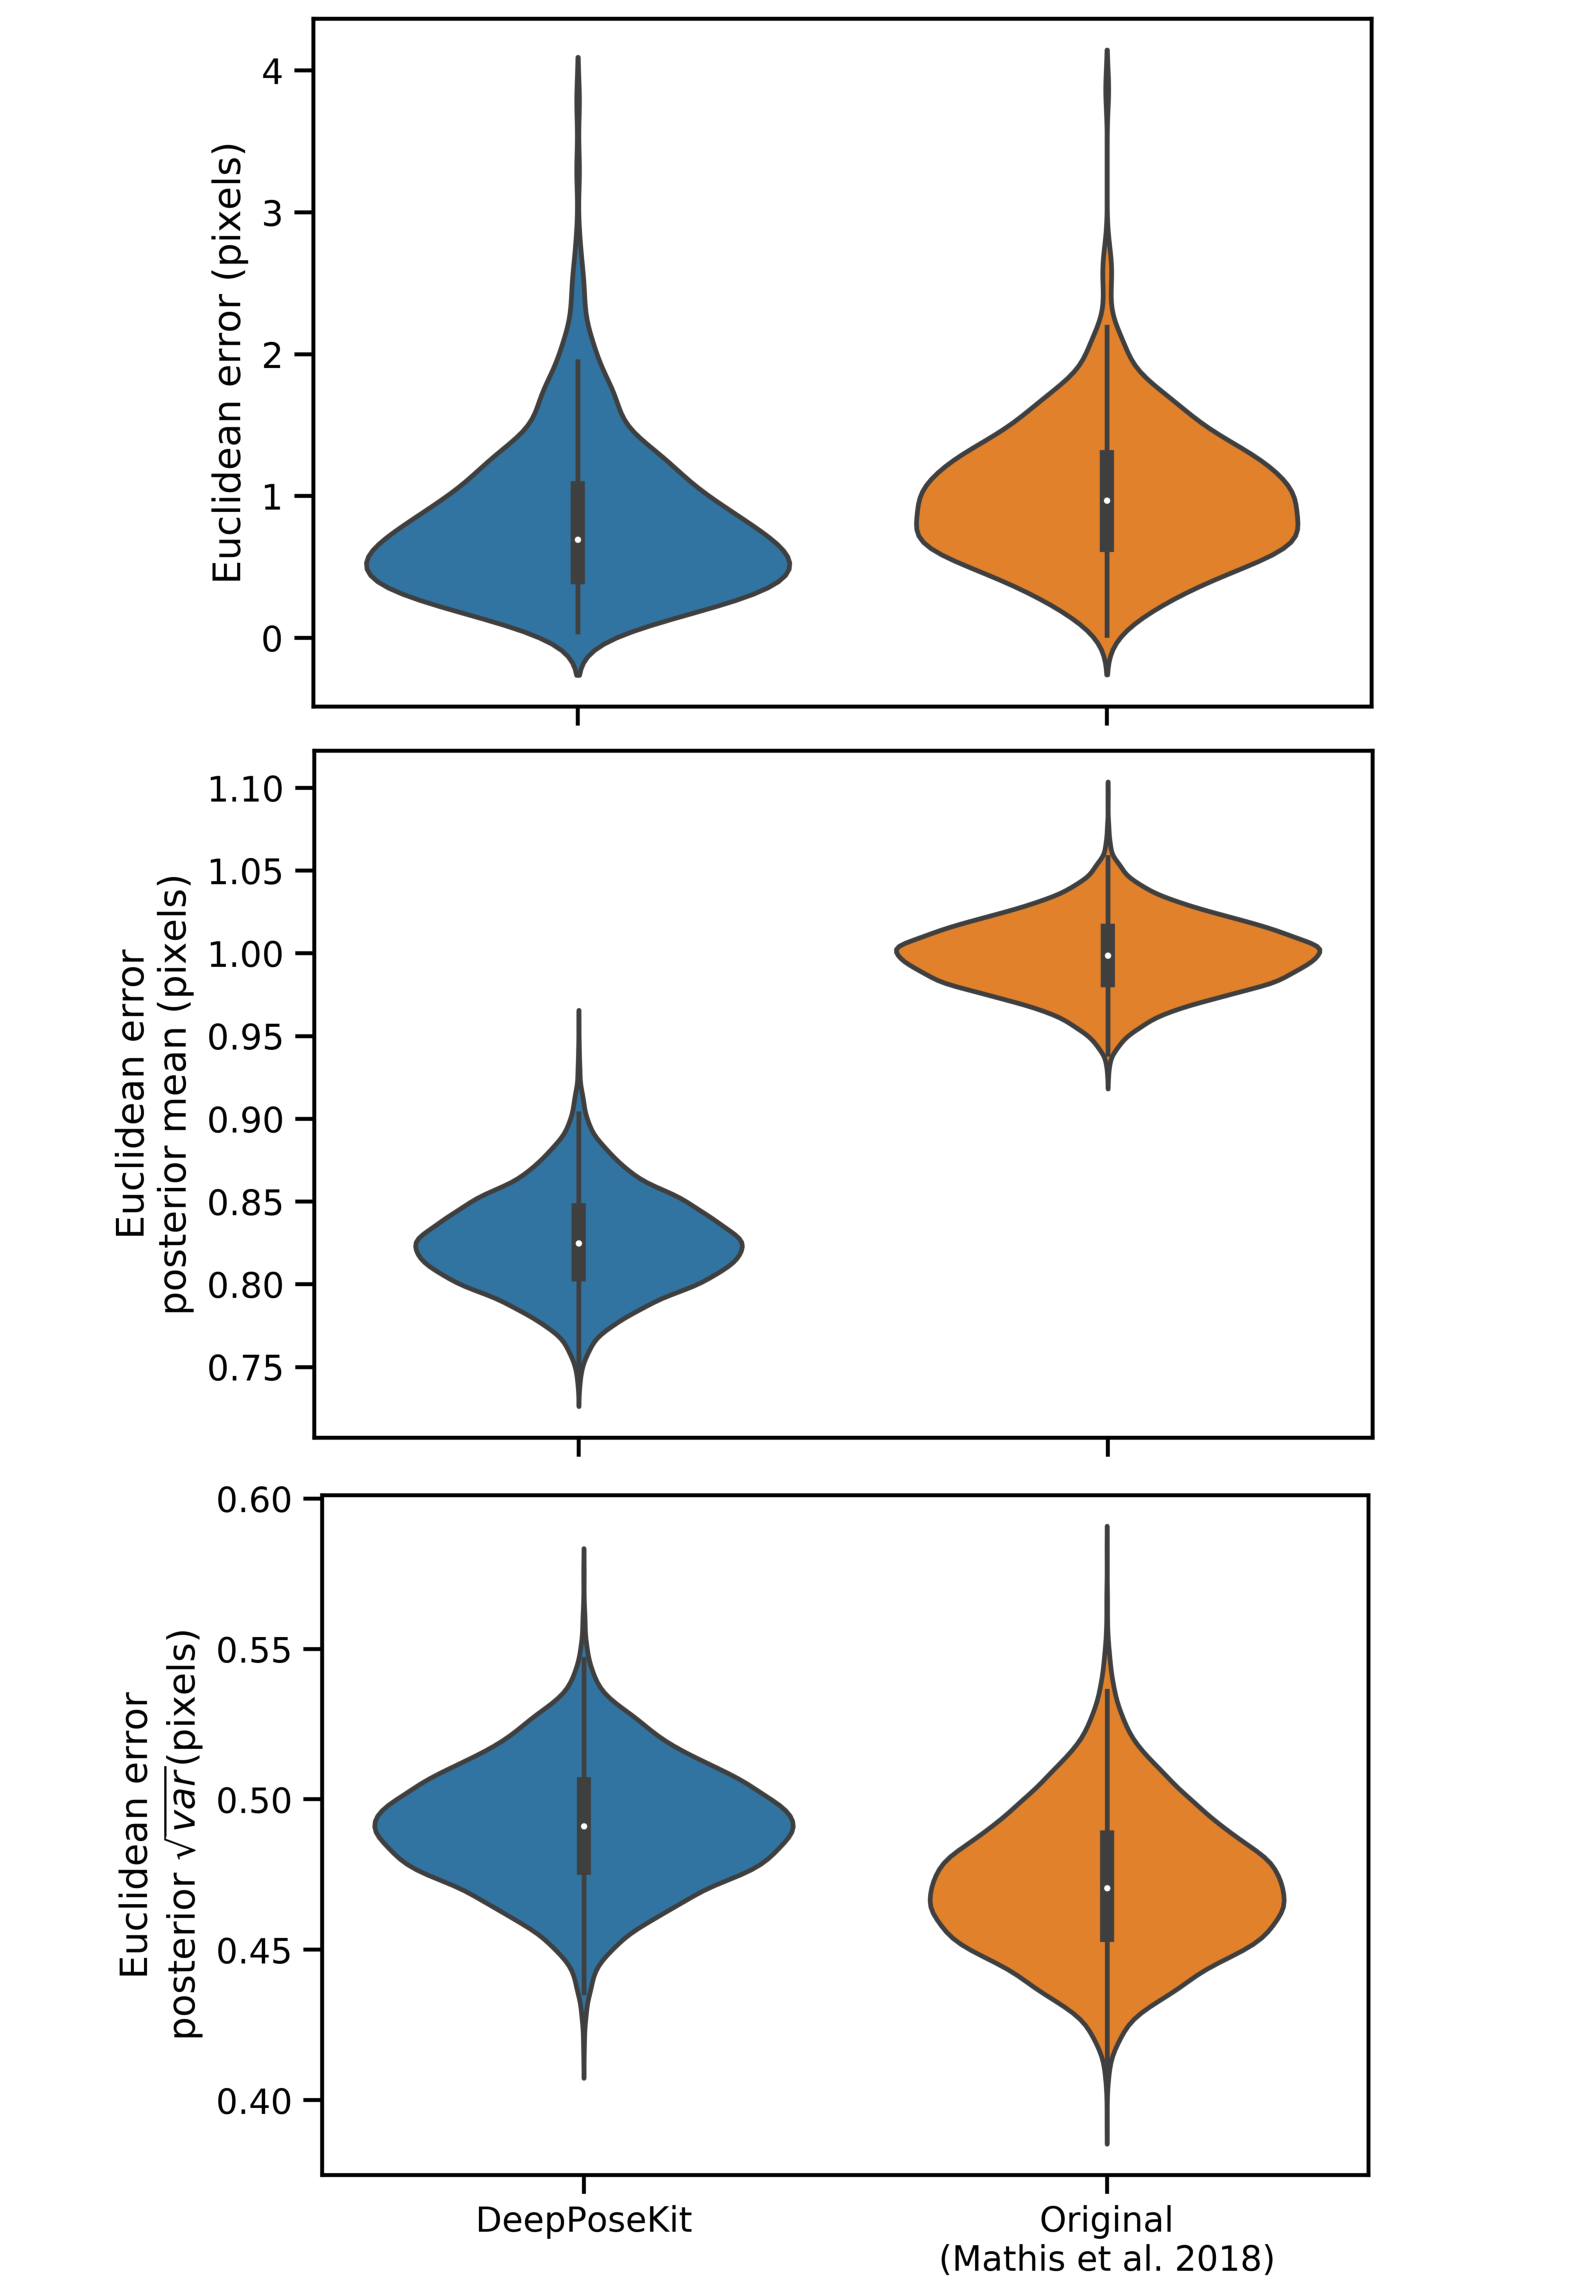
\includegraphics[width=0.8\linewidth]{Graving_IMPRS_Thesis/figures/dlc_comparison_errors.pdf}
\caption{Prediction errors for the odor-trail mouse dataset from \cite{mathis2018deeplabcut} using the original implementation of the DeepLabCut model \citep{mathis2018deeplabcut, nath2018} and our modified version of this model implemented in DeepPoseKit. Mean prediction error is slightly lower for the DeepPoseKit implementation, but there is no discernible difference in variance. These results indicate that the models achieve nearly identical prediction accuracy despite modification. We also provide qualitative comparisons of these results in Appendix \ref{app:implementation} Figure \ref{fig:dlc_comparison}-Figure supplements \ref{figsupp:dlc_tsplot} and \ref{figsupp:dlc_dxtsplot}, and Appendix \ref{app:implementation} Figure \ref{fig:dlc_comparison}-video \ref{videosupp:dlcsv1}.}
\label{fig:dlc_comparison}
\end{figure}

\begin{figure}[!htb]
    \centering
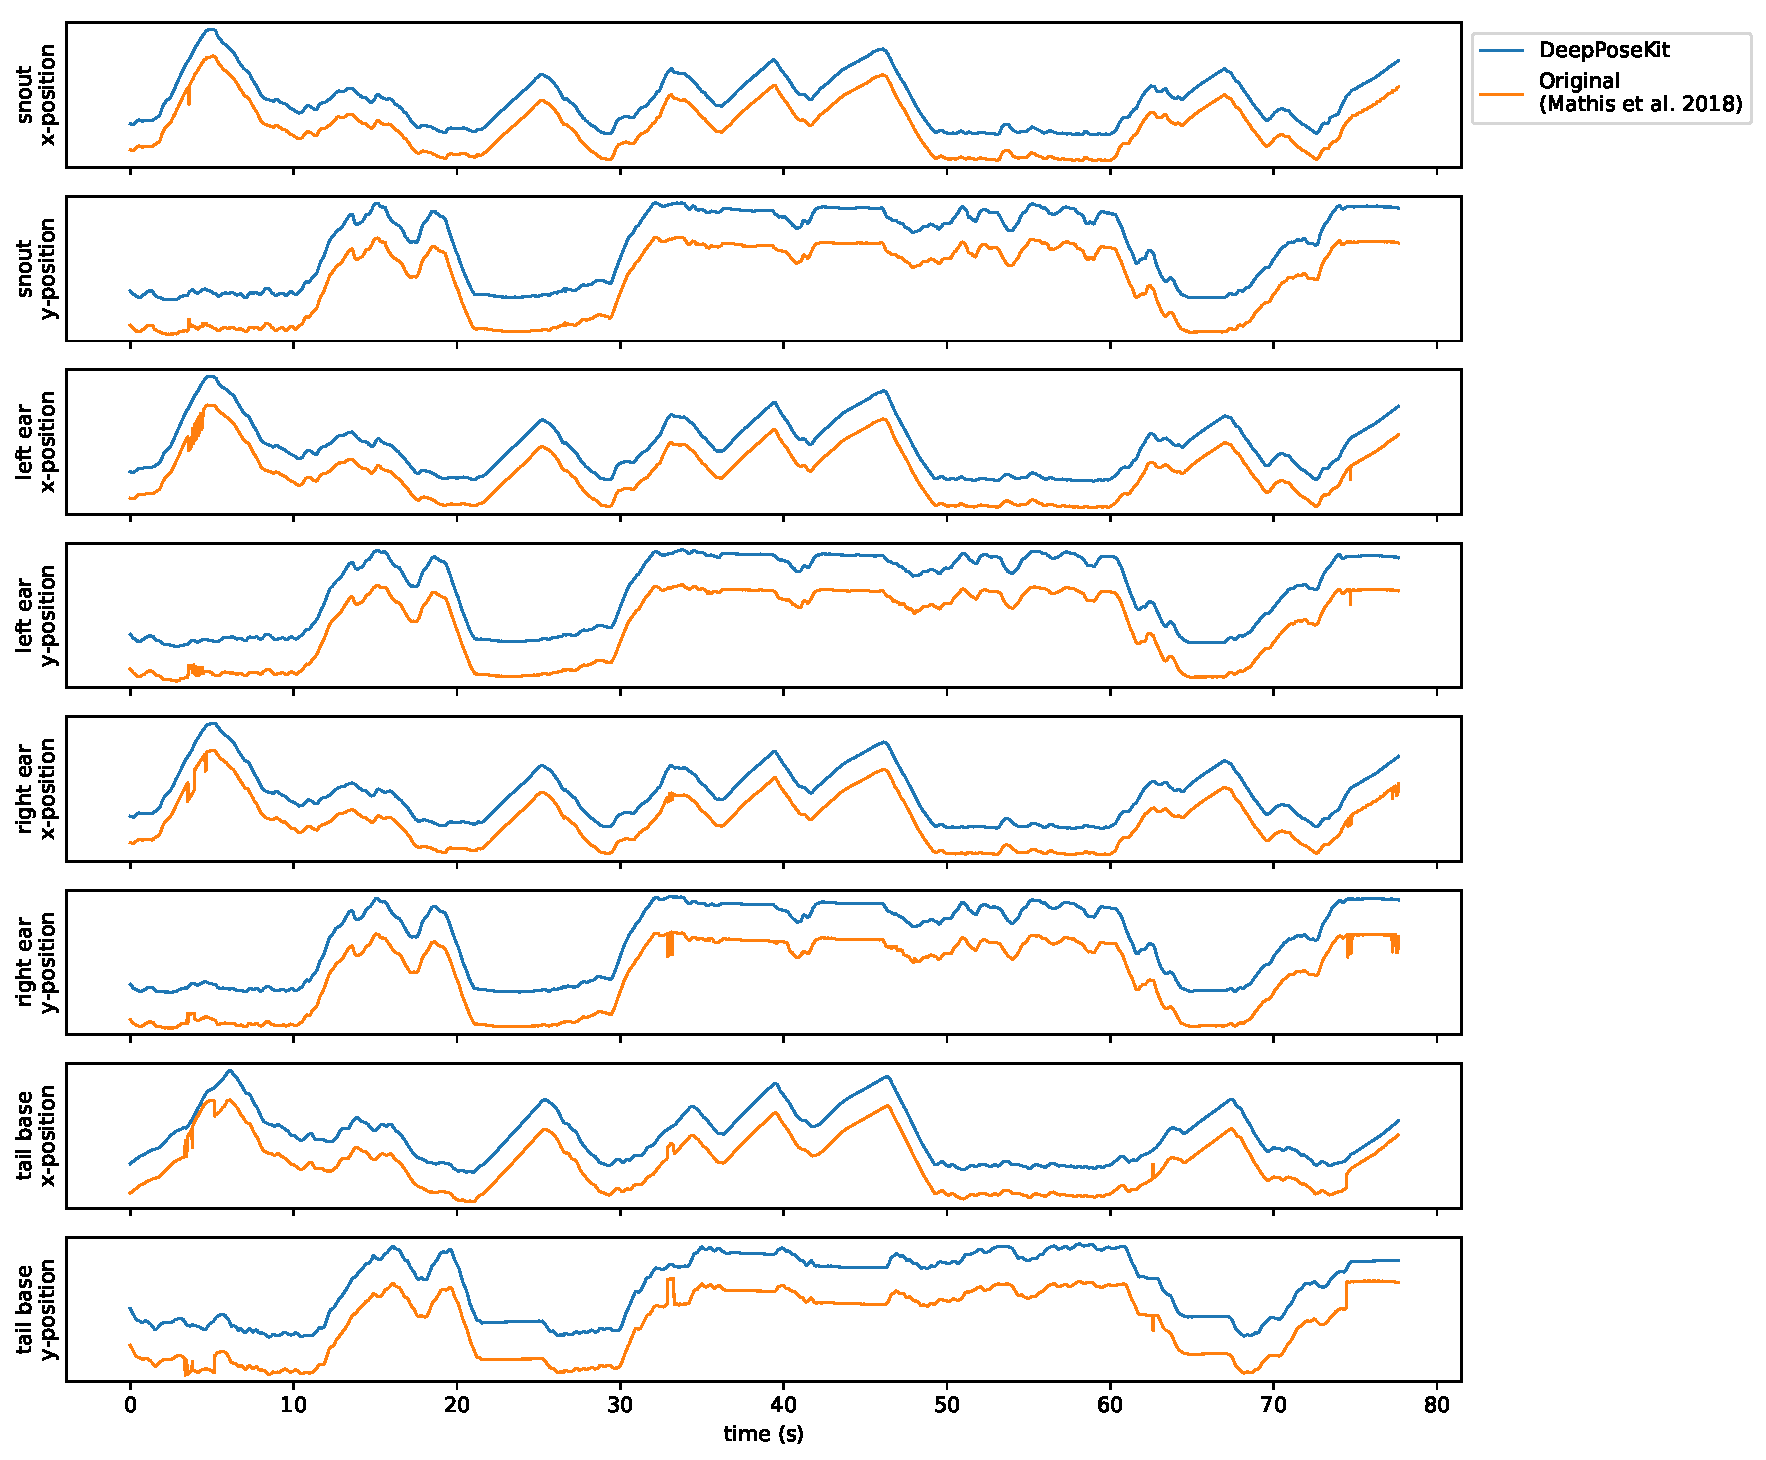
\includegraphics[width=\linewidth]{Graving_IMPRS_Thesis/figures/dlc_tsplot.pdf}    
\caption{Plots of the predicted output for Appendix \ref{app:implementation} Figure \ref{fig:dlc_comparison}-video \ref{videosupp:dlcsv1} comparing our implementation of the DeepLabCut model \citep{mathis2018deeplabcut} in DeepPoseKit vs. the original implementation from \cite{mathis2018deeplabcut, nath2018}. Note the many fast jumps in position for the original verison from \cite{mathis2018deeplabcut}, which indicates prediction errors. }
\label{figsupp:dlc_tsplot}
\end{figure}

\begin{figure}[!htb]
    \centering
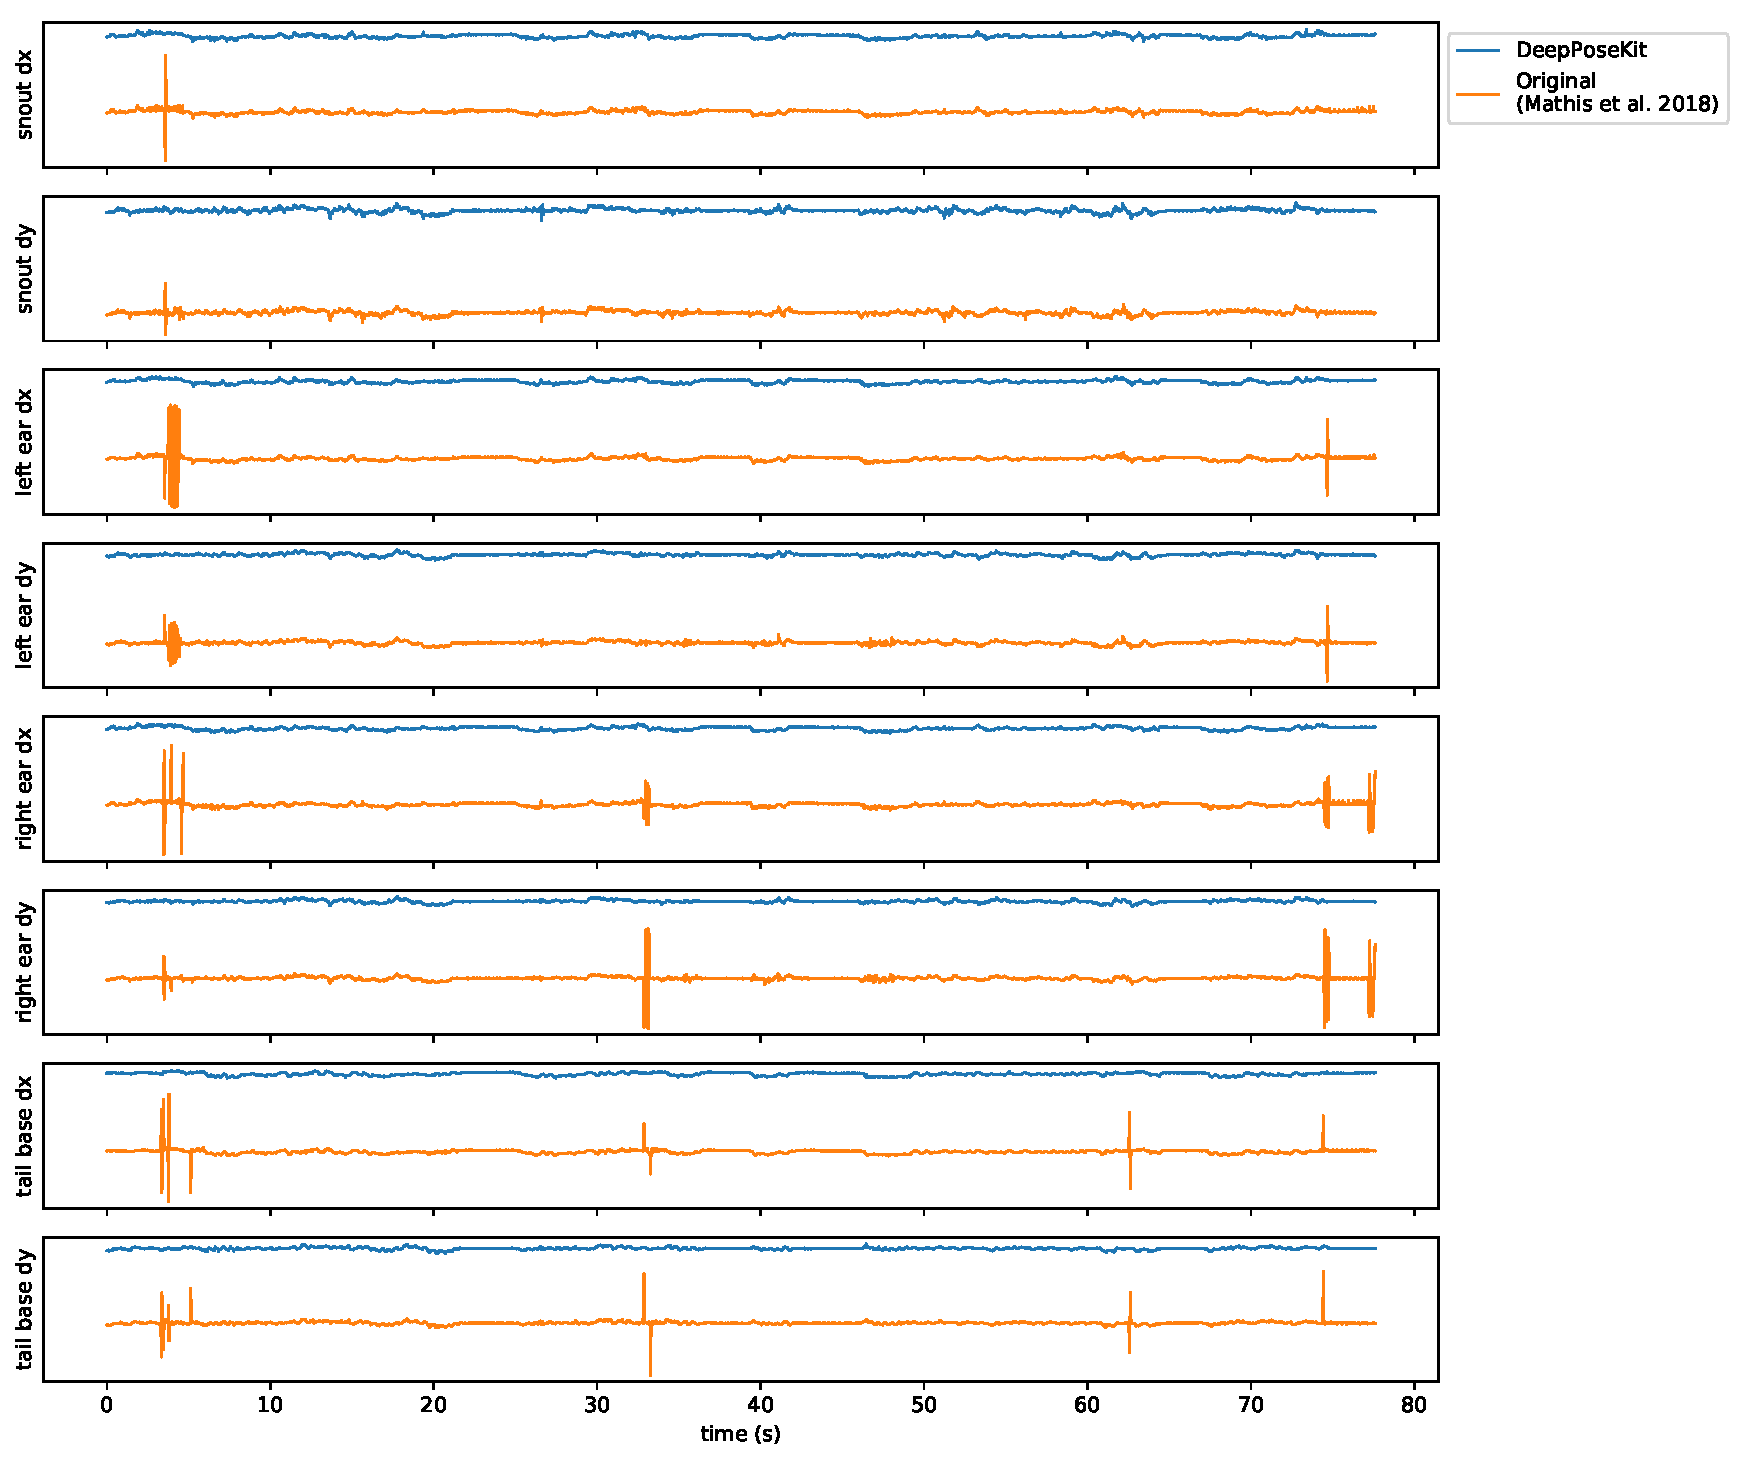
\includegraphics[width=\linewidth]{Graving_IMPRS_Thesis/figures/dlc_dxtsplot.pdf}
\caption{Plots of the temporal derivatives of the predicted output for Appendix \ref{app:implementation} Figure \ref{fig:dlc_comparison}-video \ref{videosupp:dlcsv1} comparing our implementation of the DeepLabCut model \citep{mathis2018deeplabcut} in DeepPoseKit vs. the original implementation from \cite{mathis2018deeplabcut, nath2018}. Note the many fast jumps in position for the original verison from \cite{mathis2018deeplabcut}, which indicates prediction errors}
\label{figsupp:dlc_dxtsplot}
\end{figure}

\begin{figure}[!htb]
    \centering
    \caption{A video comparison of the tracking output of our implementation of the DeepLabCut model \citep{mathis2018deeplabcut} in DeepPoseKit vs. the original implementation from \cite{mathis2018deeplabcut, nath2018}. \url{https://youtu.be/YFmO5C0hUw4}}
\label{videosupp:dlcsv1}
\end{figure}


\label{app:depthwise}
\section[Depthwise-separable convolutions]{Depthwise-separable convolutions for memory-limited applications}
In an effort to maximize model efficiency, we also experimented with replacing 3$\times$3 convolutions in our model implementations with 3$\times$3 depthwise-separable convolutions —first introduced by \cite{chollet2017xception} and now commonly used in fast, efficient “mobile” CNNs (e.g., \citealt{sandler2018mobilenetv2}). In theory this modification should both reduce the memory footprint of the model and increase inference speed. However we found that, while this does drastically decrease the memory footprint of our already memory-efficient models, it slightly decreases accuracy and does not improve inference speed, so we opt for a full 3$\times$3 convolution instead. We suspect that this discrepancy between theory and application is due to inefficient implementations of depthwise-separable convolutions in many popular deep learning frameworks, which will hopefully improve in the near future. At the moment we include this option as a hyperparameter for our Stacked DenseNet model, but we recommend using depthwise-separable convolutions only for applications that require a small memory footprint such as training on a lower-end GPU with limited memory or running inference on a mobile device.

\chapter[VAE-SNE]{Appendix to ``VAE-SNE, a deep generative model for simultaneous dimensionality reduction and clustering"}

\begin{table}[!htb]
\caption{  \textbf{Ranked information preservation metric performance for nonlinear dimension reduction algorithms}.
Rankings for each nonlinear dimension reduction algorithm in terms of general performance for local, global, fine-scale, and temporal structure preservation (lower is better).}
\resizebox{\linewidth}{!}{
\begin{tabular}{llllll}
\textbf{name}            & \textbf{citation} & \textbf{local} & \textbf{global} & \textbf{fine-scale} & \textbf{temporal} \\
VAE-SNE (t-SNE) & this paper            &  1 & 1 & 2 & 2 \\
VAE-SNE (SNE)   & this paper            & 2 &  1 & 2 &  1 \\
FIt-SNE         & Linderman et al. (2017) &  1 & 2 &  1 & 2 \\
Barnes-Hut-SNE & van der Maaten (2014) &  1               & 2                &  1                    & 2                  \\
UMAP (LE init)            & McInnes et al. (2018)   &  1 & 3 & 2 & 3 \\
UMAP (PCA init)            & McInnes et al. (2018)   &  1 & 2 & 2 & 3 \\
scvis           & Ding et al. (2018)     & 2 &  1 & 2 & 2 \\
ivis            & Szubert et al. (2019)   & 2 &  1 & 3 &  1 \\
\end{tabular}
}
\label{table:info}

\end{table}

\begin{table}[!htb]
\caption{  \textbf{Ranked processing speed performance for nonlinear dimension reduction algorithms}. Rankings for each nonlinear dimension reduction algorithm in terms of general performance for training time and test time (lower is better), as well as whether or not test time increases as a function of training set size.}
\resizebox{\linewidth}{!}{
\begin{tabular}{lllll}
\textbf{name}            & \textbf{citation}                  & \textbf{train time} & \textbf{test time} & \textbf{test time $\propto$ train size} \\
VAE-SNE         & this paper                 & 4          & 1         & no                           \\
FIt-SNE         & Linderman et al. (2017)      & 2          & 4         & no                           \\
Barnes-Hut-SNE  & van der Maaten (2014) & 3          & 5         & yes                          \\
UMAP            & McInnes et al. (2018)        & 1          & 3         & yes                          \\
scvis           & Ding et al. (2018)          & 6          & 1         & no                           \\
ivis            & Szubert et al. (2019)        & 5          & 2         & no                          
\end{tabular}
}
\label{table:speed}
\end{table}

\begin{table}[!htb]
\caption{  \textbf{Additional features for nonlinear dimension reduction algorithms}. A summary of potentially useful additional features for each nonlinear dimension reduction algorithm including batch training for applying dimension reduction to large out-of-core datasets, non-Euclidean embeddings for different types of compressed representations, whether the algorithm is tractable in higher dimensions ($>$2), and whether the algorithm learns a distribution of clusters within the data.}
\resizebox{\linewidth}{!}{
\begin{tabular}{llllll}
\textbf{name}             & \textbf{citation}                   & \textbf{batch training} & \textbf{non-Euclidean} & \textbf{$>$2 dims.} & \textbf{clustering} \\
VAE-SNE & this paper                 & yes            & yes        & yes           & yes             \\
FIt-SNE         & Linderman et al. (2017)      & no             & no                       & no            & no              \\
Barnes-Hut-SNE  & van der Maaten (2014) & no             & no                       & yes           & no              \\
UMAP            & McInnes et al. (2018)        & no             & yes                      & yes           & no              \\
scvis           & Ding et al. (2018)          & yes            & no                       & yes           & no              \\
ivis            & Szubert et al. (2019)        & yes            & no                       & yes           & no             
\end{tabular}
}
\label{table:features}
\end{table}


\begin{figure}[!htb]
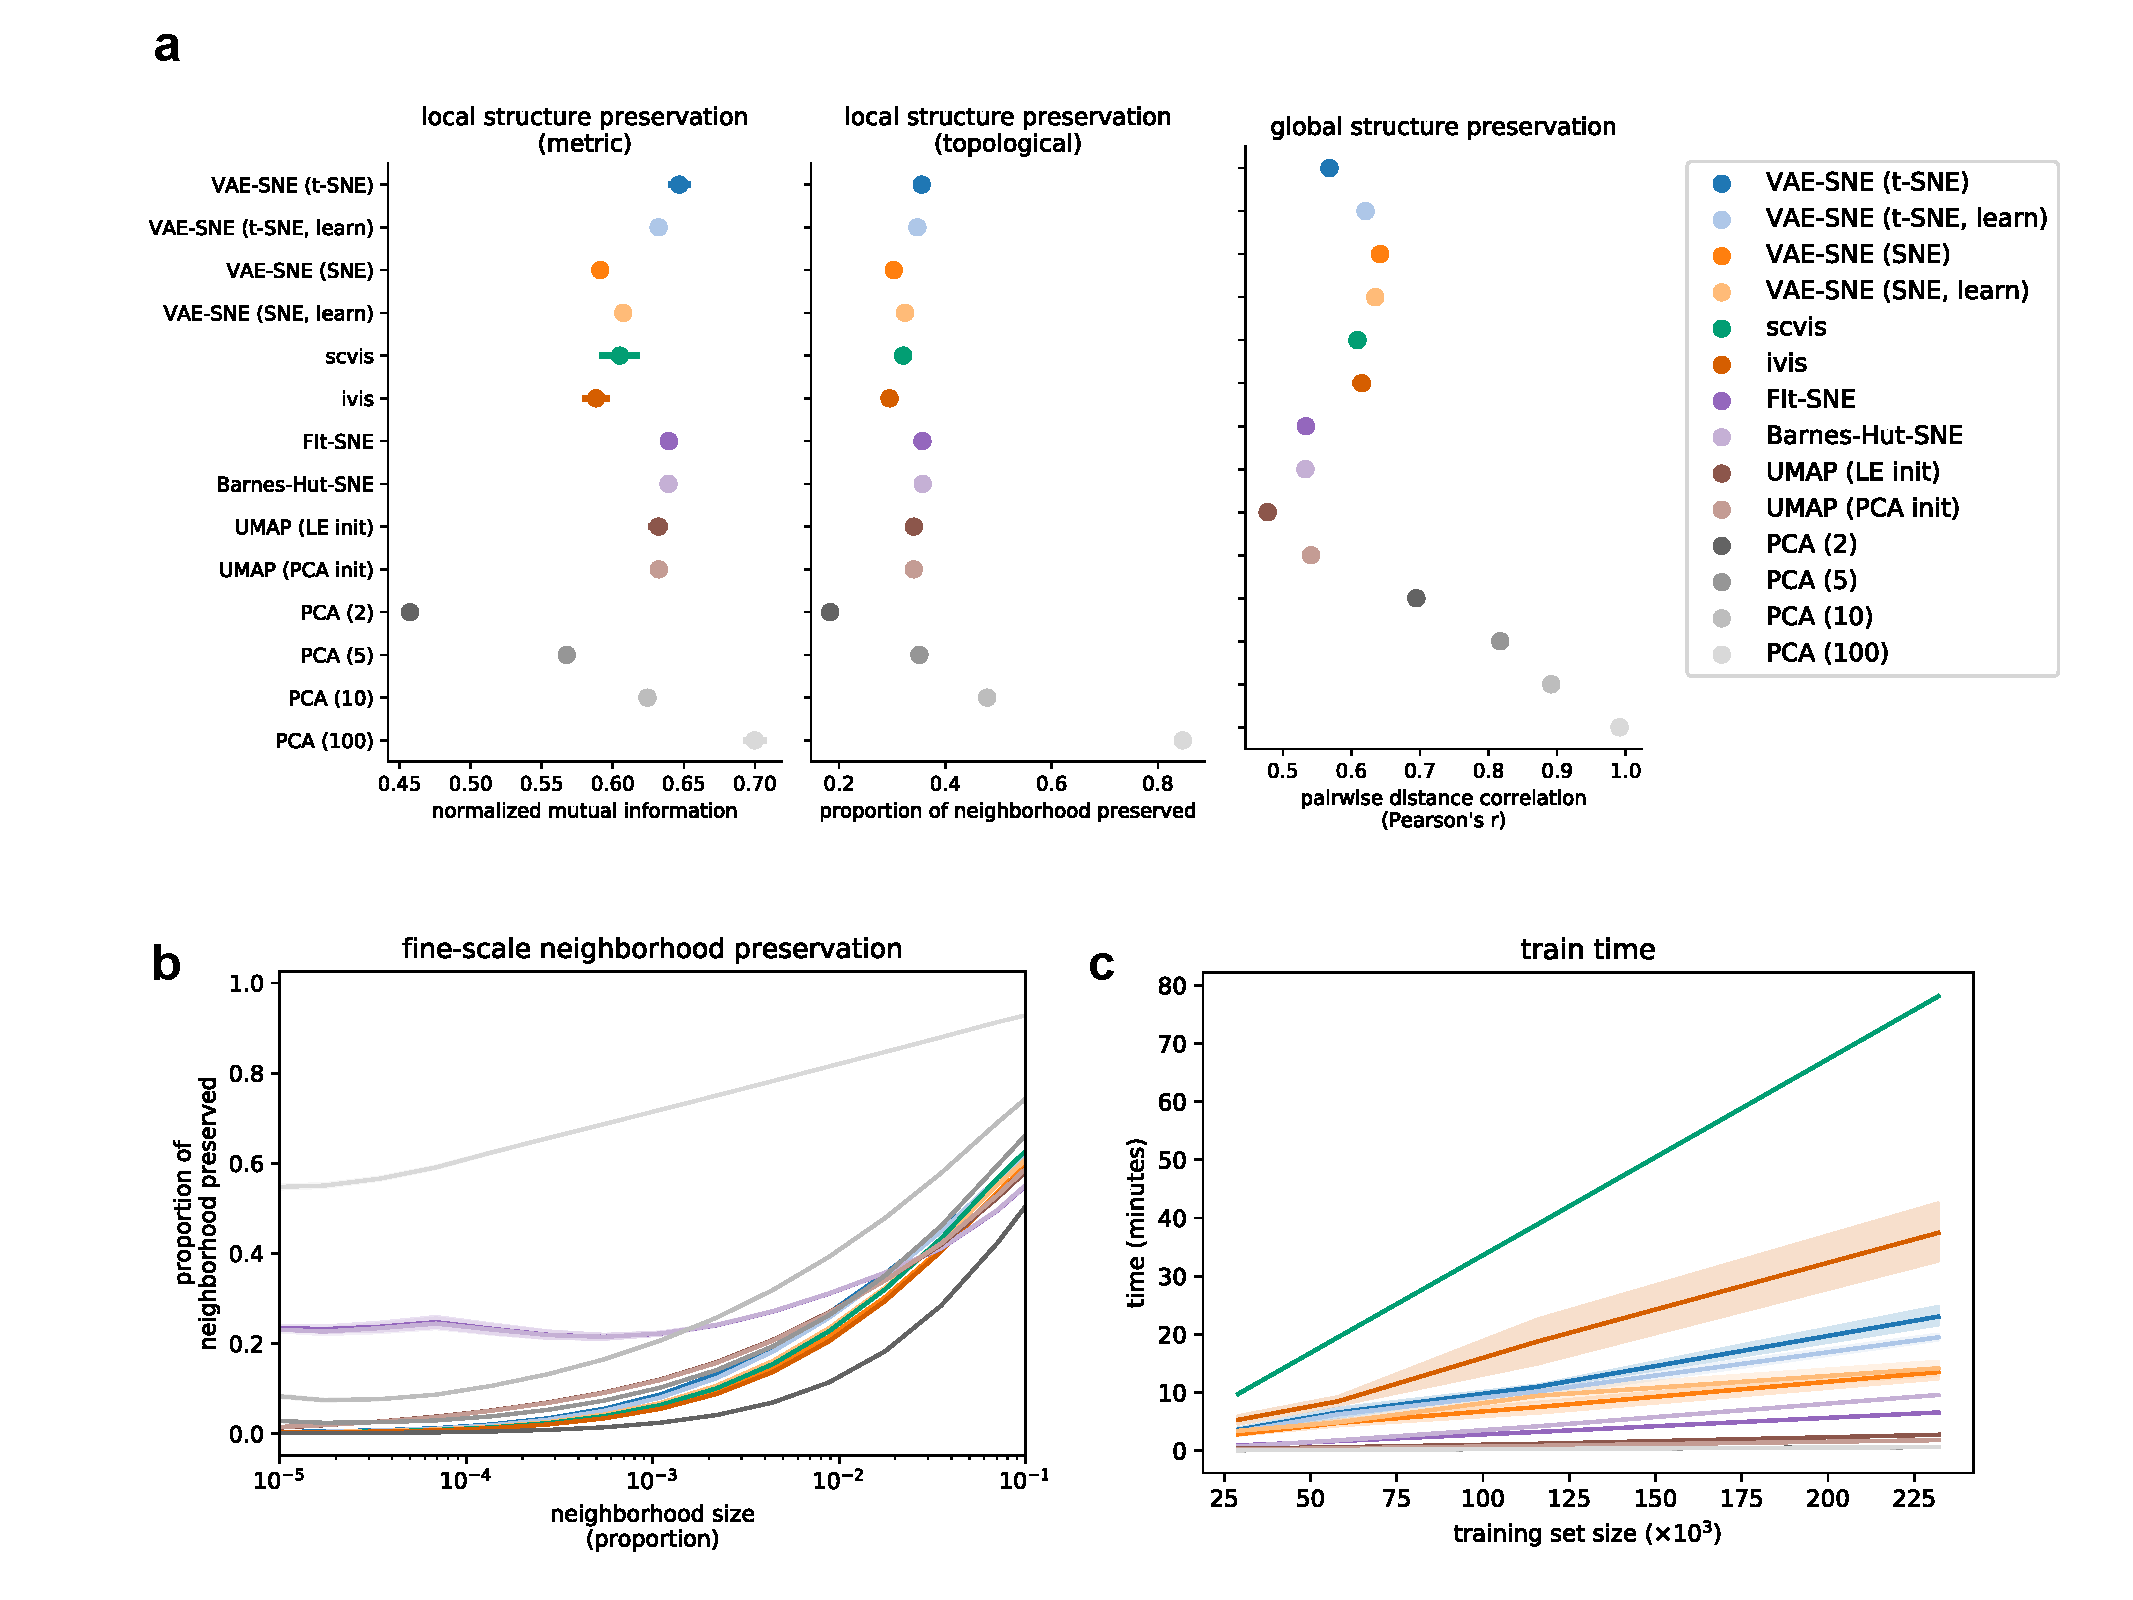
\includegraphics[width=\textwidth]{Graving_IMPRS_Thesis/figures/training_set_figure.pdf}

\caption{  \textbf{Dimension reduction performance for the posture dynamics training set}. Plots show performance comparisons for the posture dynamics dataset \citep{berman2014mapping, berman2016predictability, pereira2019fast} using the training set. \textbf{a}, Mean and 95\% interval of the bootstrap distribution for local and global structure preservation. Results are pooled across all training set sizes (for each metric n = 4 training set sizes $\times$ 5 trials $\times$ 5 replicates = 100 per algorithm). \textbf{b}, Mean and 95\% interval of the bootstrap distribution for fine-scale structure preservation across multiple neighbor sizes (as a proportion of the total embedding size). Results are from the largest training set size only (n = 14 neighborhood sizes $\times$ 5 trials $\times$ 5 replicates = 350 per algorithm). \textbf{c}, Training time for fitting each algorithm across different training set sizes (n = 4 training set sizes $\times$ 5 trials = 20 per algorithm).}

\label{fig:training_set_figure} % \label works only AFTER \caption within figure environment

\end{figure}

\begin{figure}[!htb]
\centering
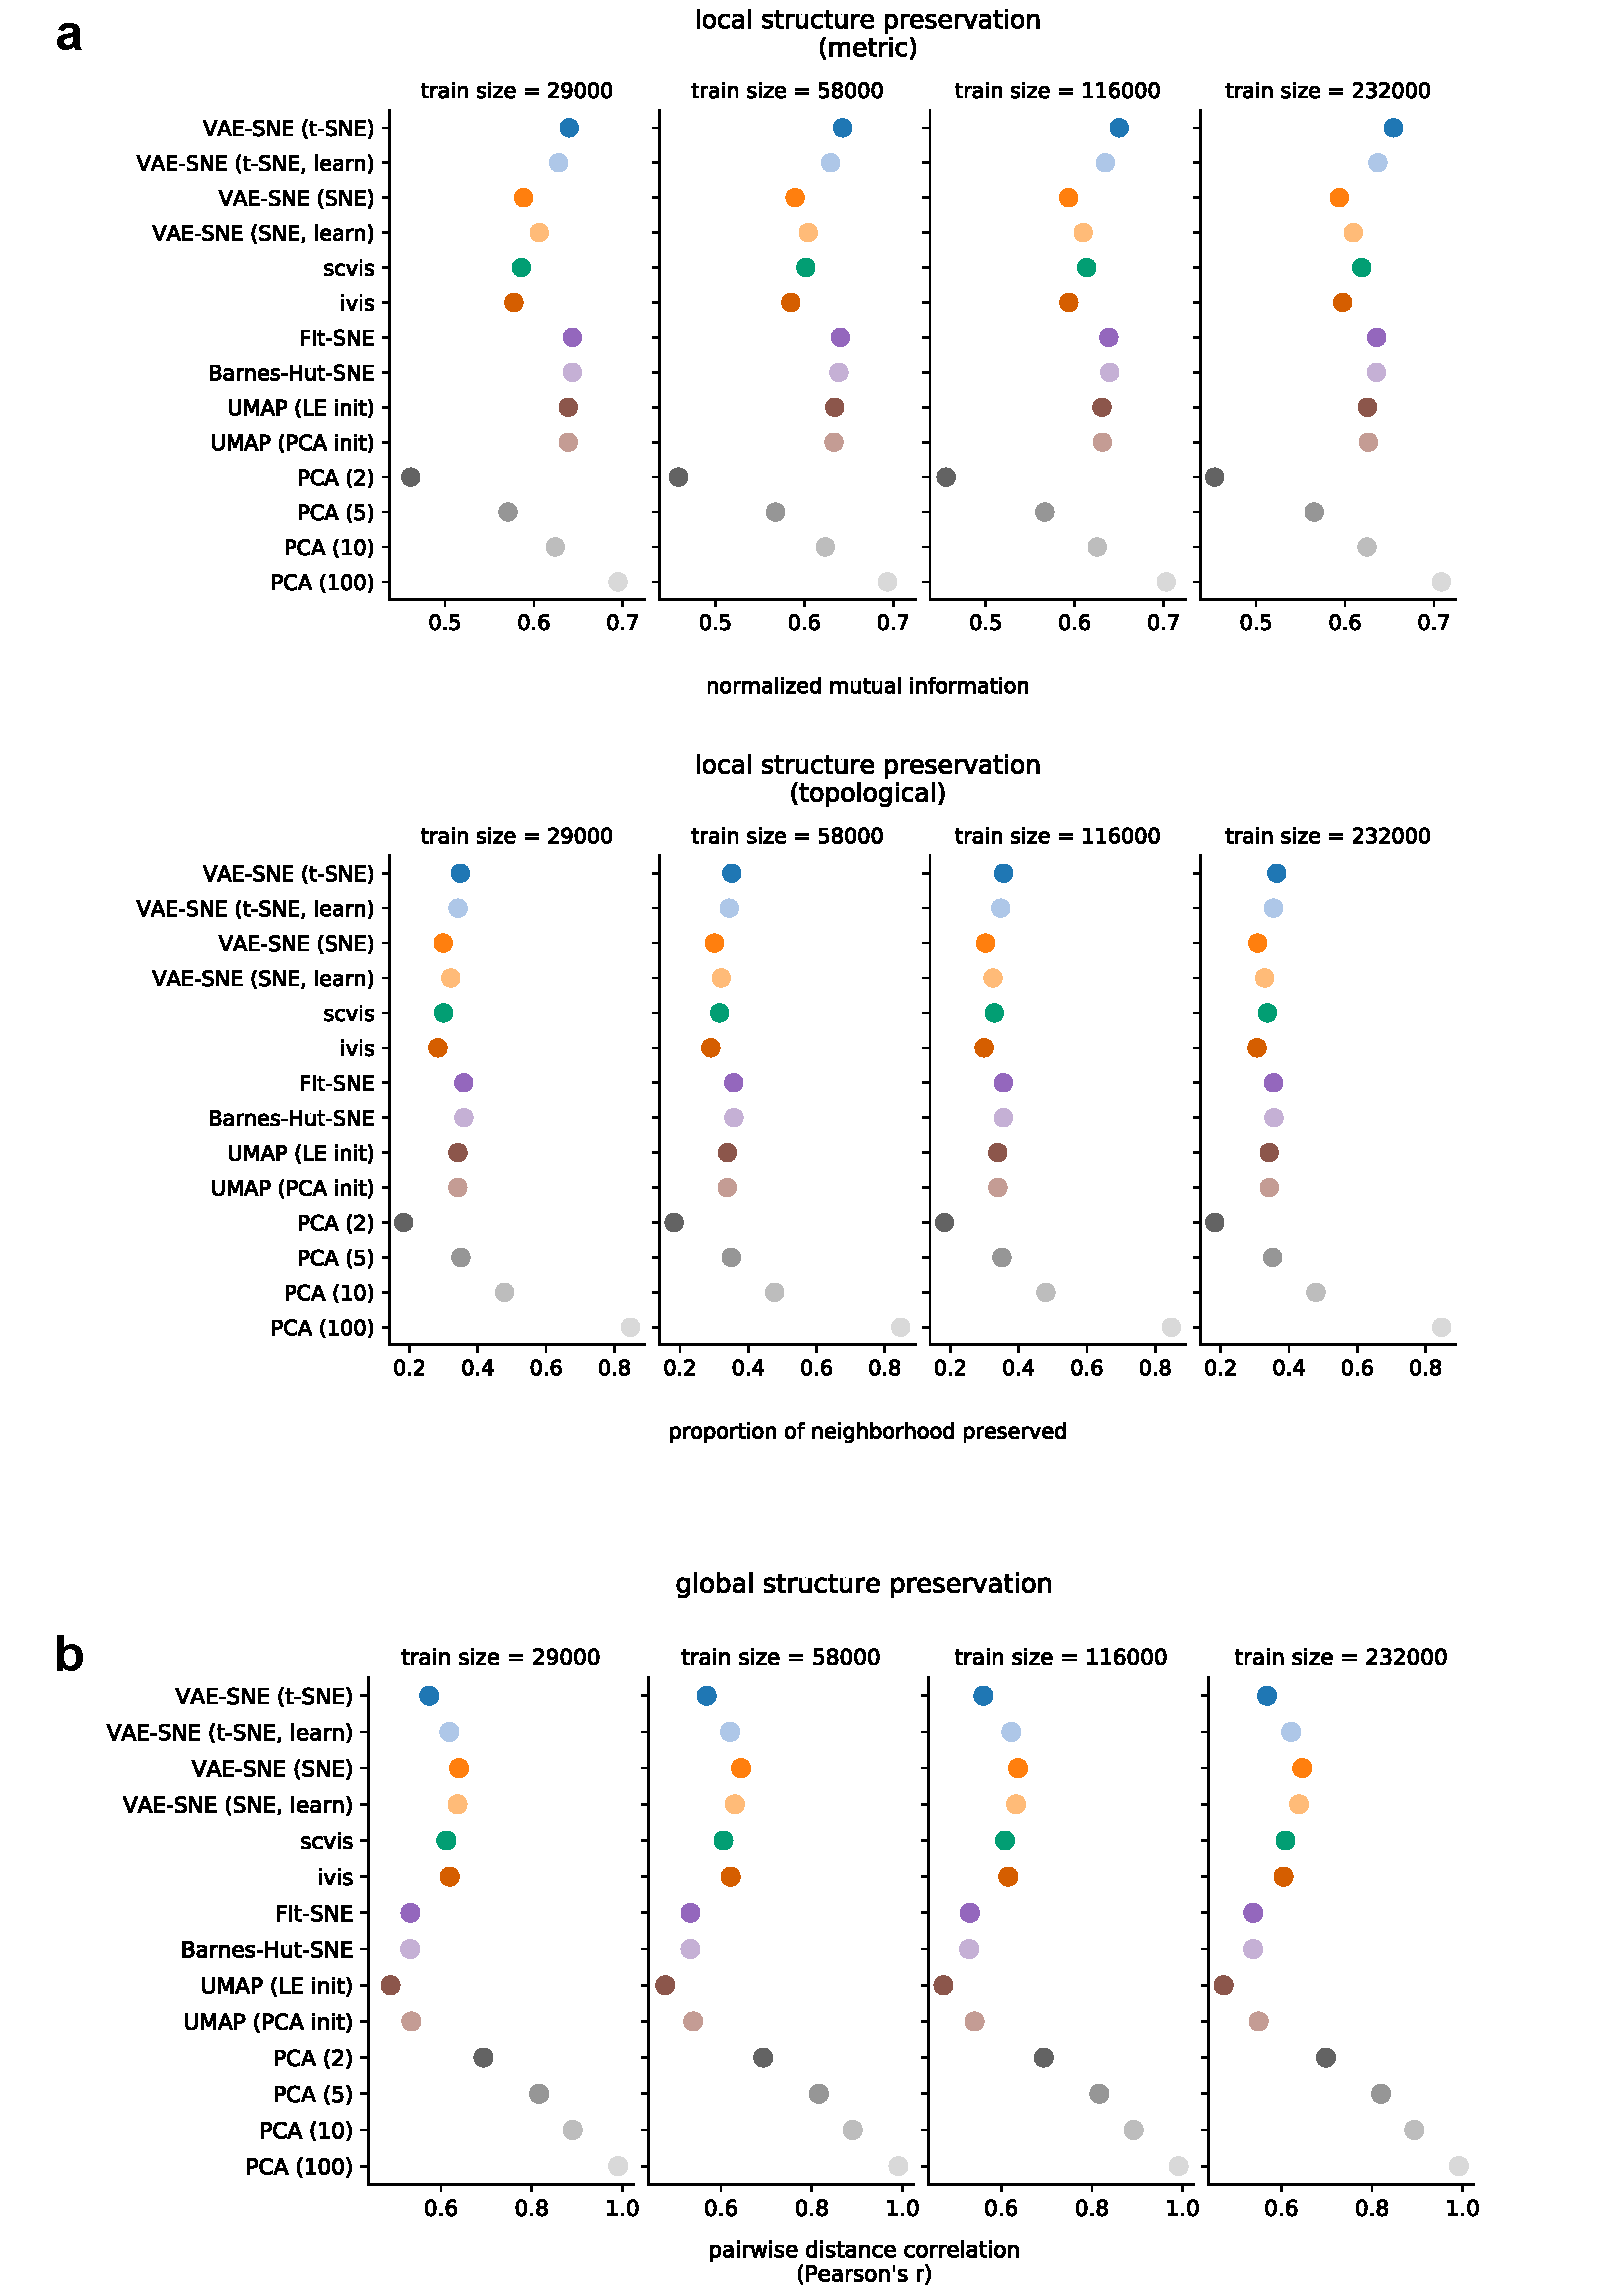
\includegraphics[width=0.9\textwidth]{Graving_IMPRS_Thesis/figures/training_set_appendix_figure.pdf}

\caption{  \textbf{Dimension reduction performance for the posture dynamics training set across training set sizes}. Plots show performance comparisons for the posture dynamics dataset \citep{berman2014mapping, berman2016predictability, pereira2019fast} using training sets of different sizes. \textbf{a-b}, Mean and 95\% interval of the bootstrap distribution for local (\textbf{a}) and global (\textbf{b}) structure preservation. (for each metric n = 5 trials $\times$ 5 replicates = 25 per training set size per algorithm)}

\label{fig:training_set_appendix_figure} % \label works only AFTER \caption within figure environment

\end{figure}



\begin{figure}[!htb]
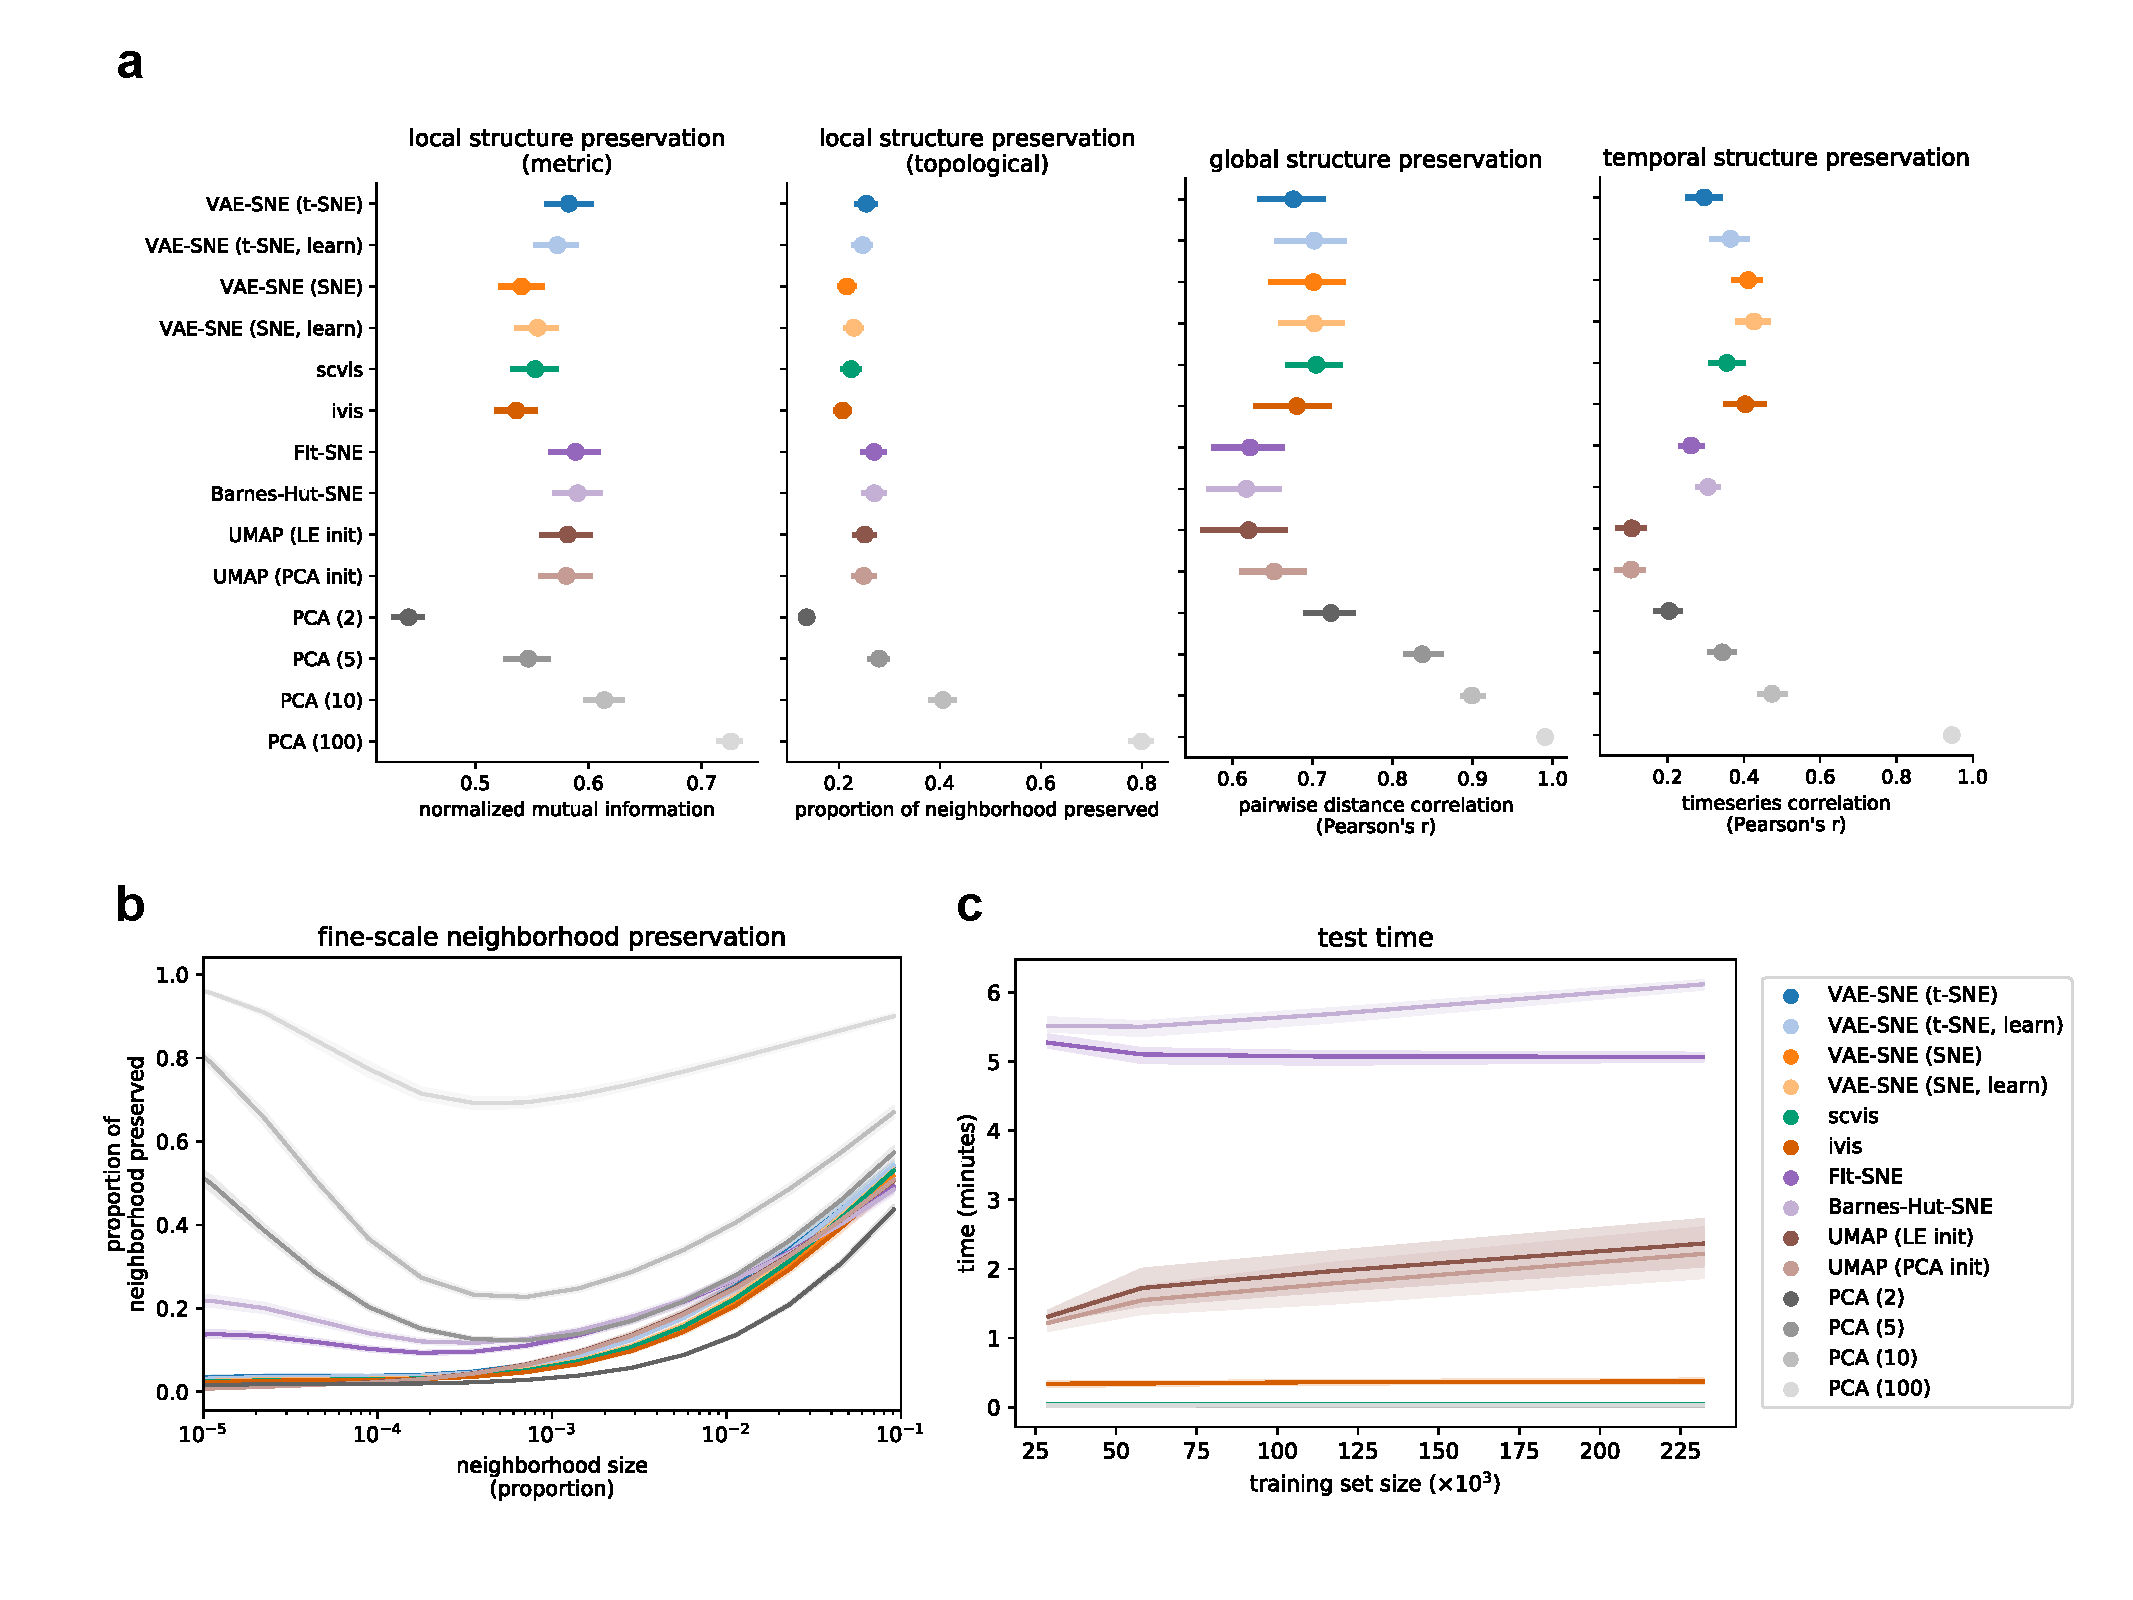
\includegraphics[width=\textwidth]{Graving_IMPRS_Thesis/figures/test_set_figure.pdf}

\caption{  \textbf{Dimension reduction performance for the posture dynamics test set}. Plots show performance comparisons for the posture dynamics dataset \citep{berman2014mapping, berman2016predictability, pereira2019fast} using the test set. \textbf{a}, Mean and 95\% interval of the bootstrap distribution for local, global, and temporal structure preservation. Results are pooled across all training set sizes (for local and global structure n = 4 training set sizes $\times$ 5 trials $\times$ 5 replicates = 100 per algorithm; for temporal structure n = 4 training set sizes $\times$ 5 trials $\times$ 50 subsamples = 1000 per algorithm). \textbf{b}, Mean and 95\% interval of the bootstrap distribution for fine-scale structure preservation across multiple neighbor sizes (as a proportion of the total embedding size). Results are from the largest training set size only (n = 14 neighborhood sizes $\times$ 5 trials $\times$ 5 replicates = 350 per algorithm). \textbf{c}, Elapsed time for embedding the test set with each algorithm across different training set sizes (n = 4 training set sizes $\times$ 5 trials = 20 per algorithm).}

\label{fig:test_set_figure} % \label works only AFTER \caption within figure environment

\end{figure}

\begin{figure}[!htb]
\centering
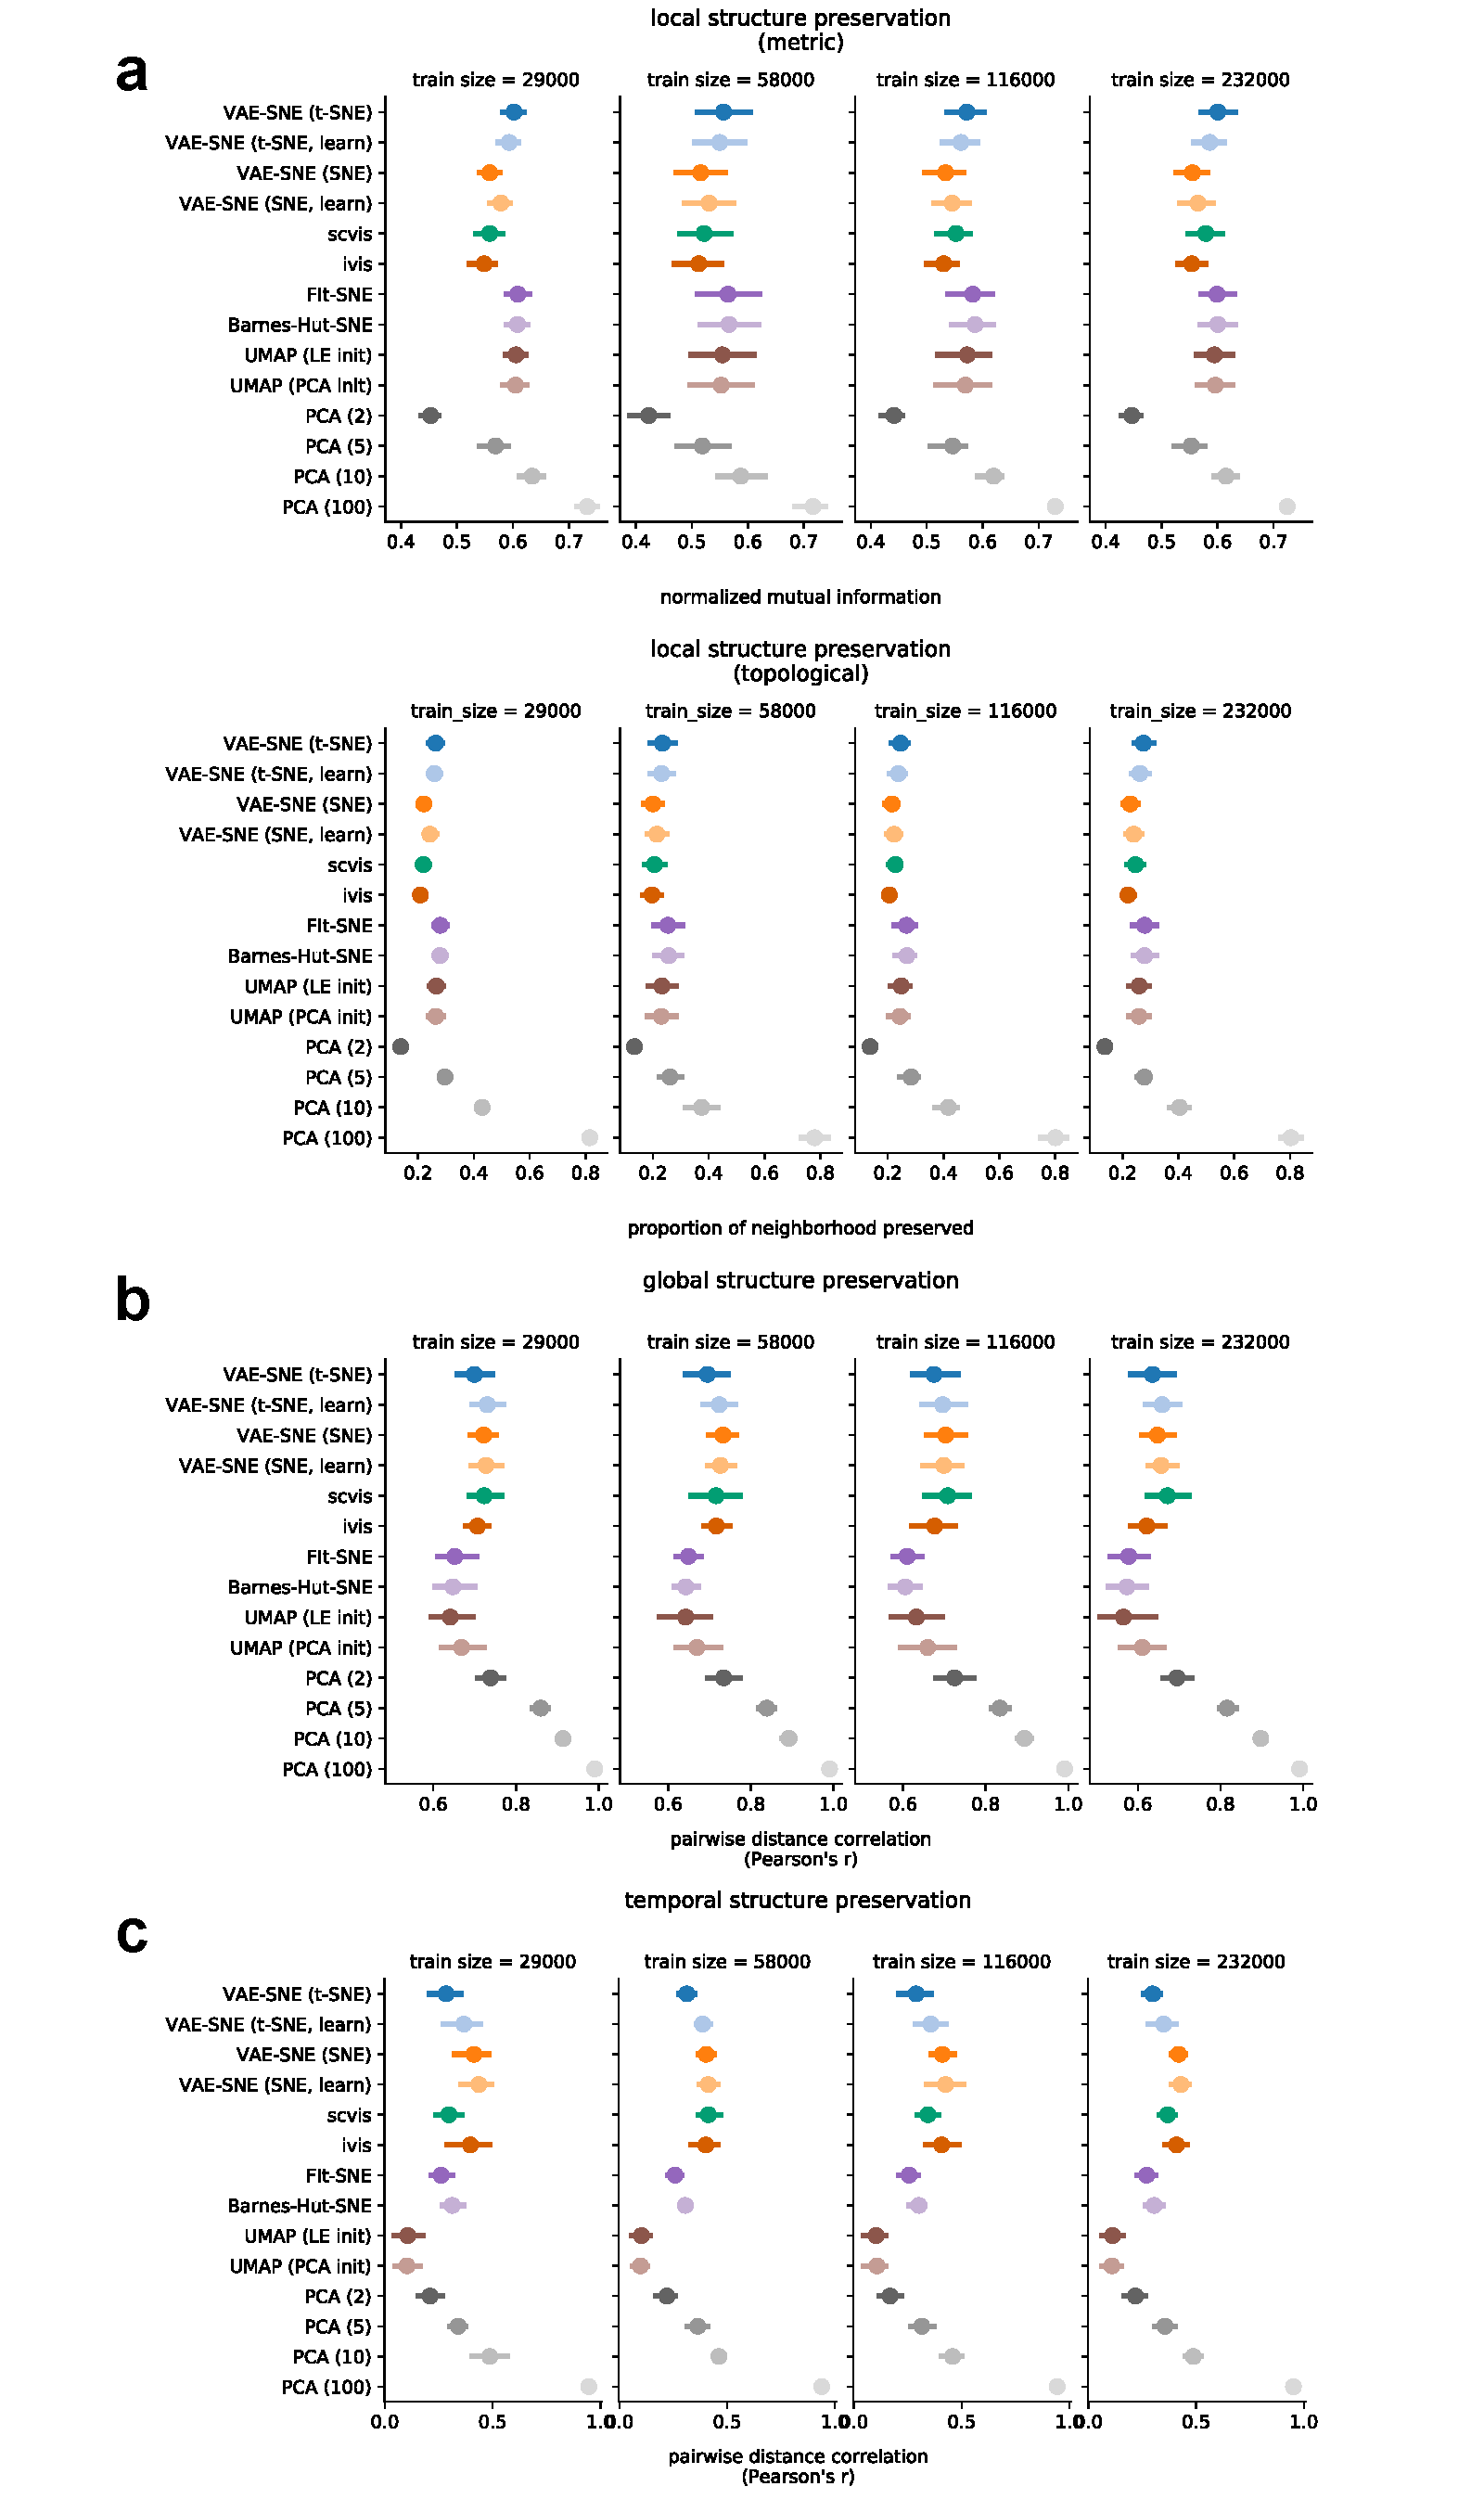
\includegraphics[width=0.75\textwidth]{Graving_IMPRS_Thesis/figures/test_set_appendix_figure.pdf}

\caption{  \textbf{Dimension reduction performance for the posture dynamics test set across training set sizes}. Plots show performance comparisons for the posture dynamics dataset \citep{berman2014mapping, berman2016predictability, pereira2019fast} using training sets of different sizes. \textbf{a-c}, Mean and 95\% interval of the bootstrap distribution for local (\textbf{a}), global (\textbf{b}), and temporal (\textbf{c}) structure preservation (for local and global structure n = 5 trials $\times$ 5 replicates = 25 per algorithm for each training set size; for temporal structure n = 5 trials $\times$ 50 subsamples = 250 per algorithm for each training set size).}

\label{fig:test_set_appendix_figure} % \label works only AFTER \caption within figure environment

\end{figure}


\begin{figure}[!htb]
\begin{center}
    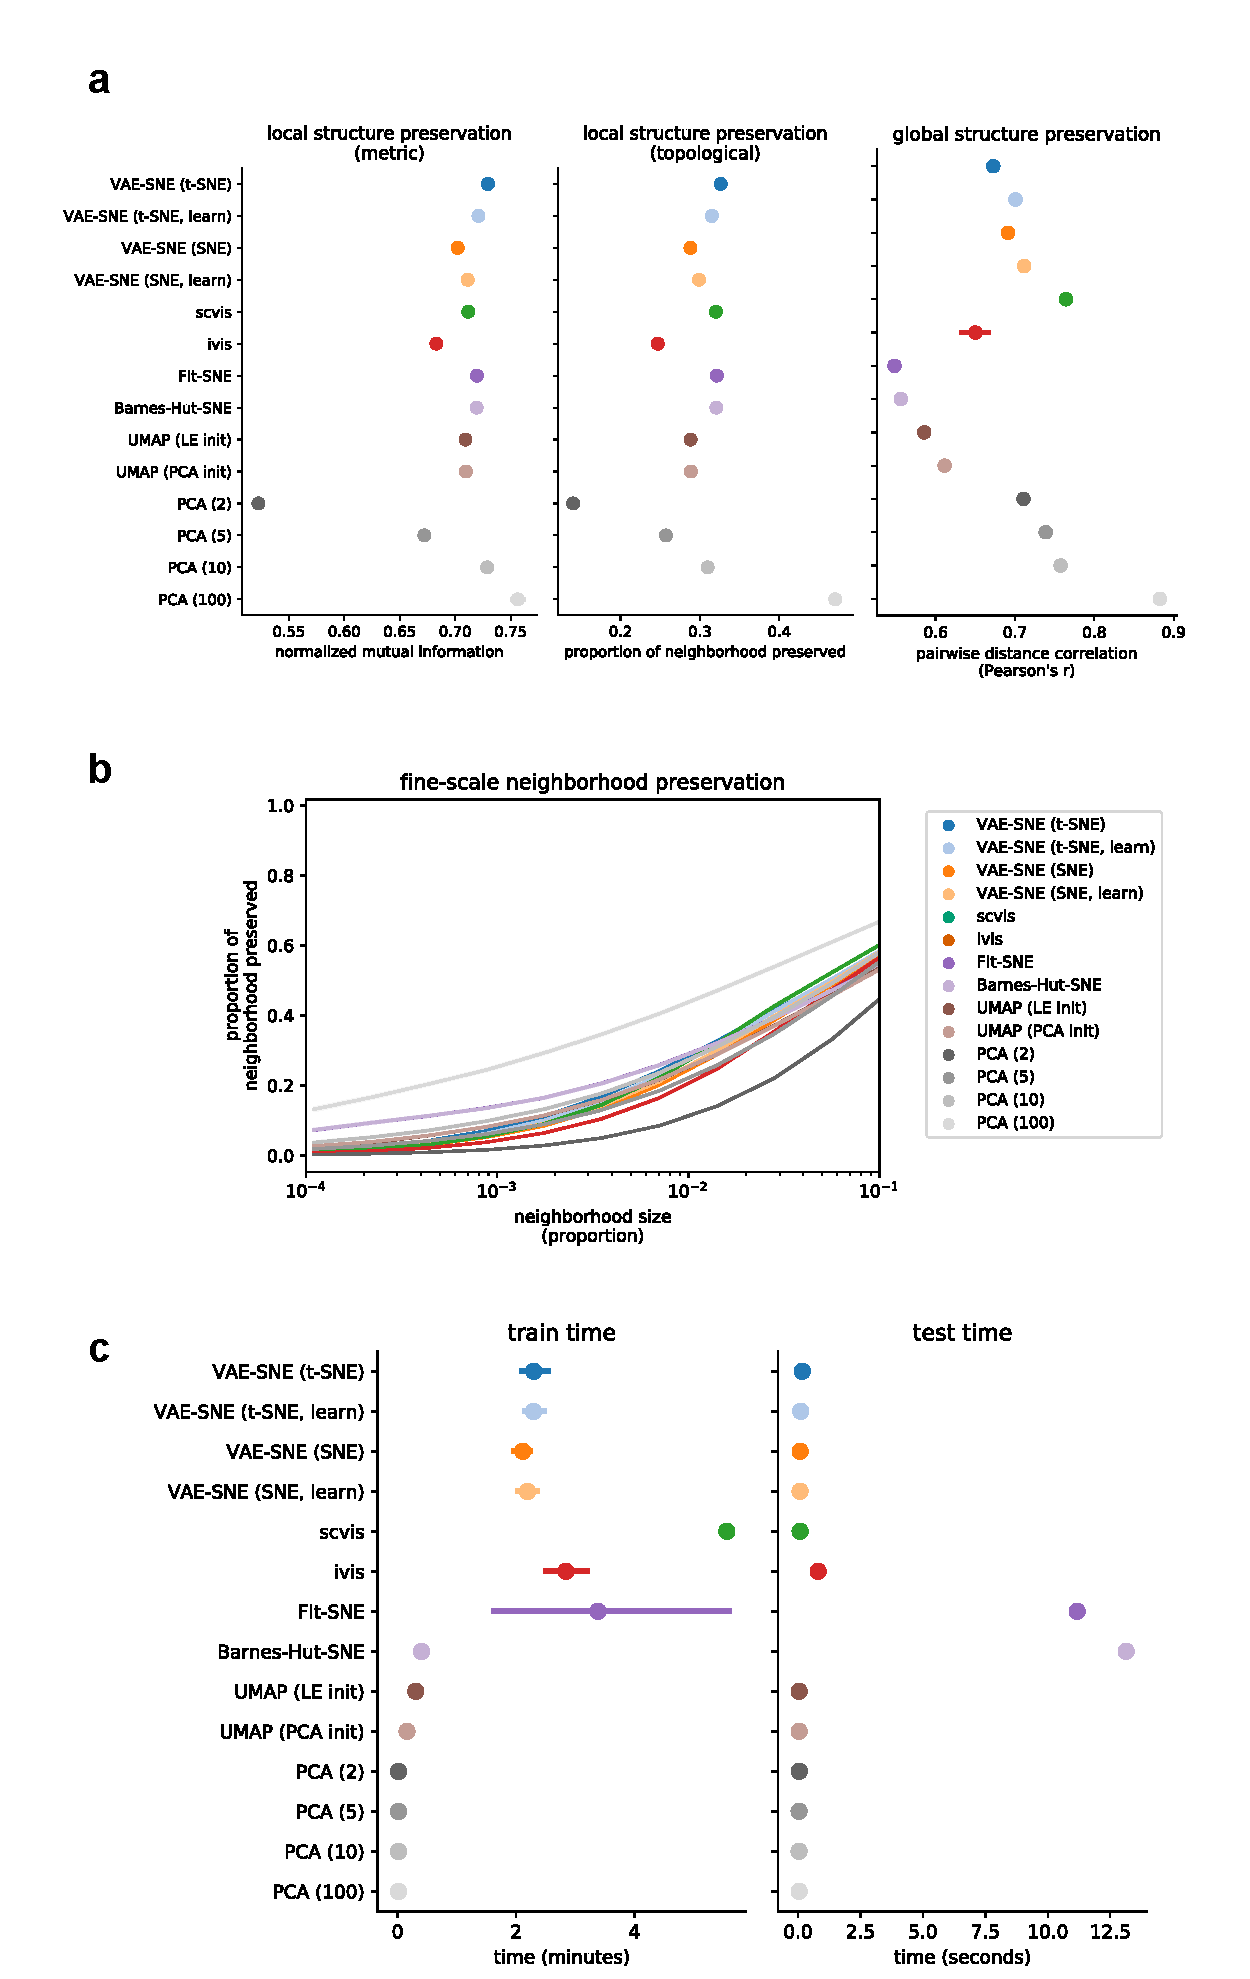
\includegraphics[width=0.7\textwidth]{Graving_IMPRS_Thesis/figures/rna_velocity_figure.pdf}
\end{center}

\caption{  \textbf{Dimension reduction performance for the single-cell RNA-seq dataset}. Plots show performance comparisons for the single-cell RNA-seq dataset from \cite{la2018rna} using the entire dataset. \textbf{a}, Mean and 95\% interval of the bootstrap distribution for local and global structure preservation (for each metric n = 5 trials $\times$ 5 replicates = 25 per algorithm). \textbf{b}, Mean and 95\% interval of the bootstrap distribution for fine-scale structure preservation across multiple neighbor sizes (as a proportion of the total embedding size; n = 14 neighborhood sizes $\times$ 5 trials $\times$ 5 replicates = 350 per algorithm). \textbf{c}, Elapsed time for embedding the training set and re-embedding the training set as a ``test" set with each algorithm (for each metric n = 5 trials $\times$ 5 replicates = 25 per algorithm).}

\label{fig:rna_velocity_figure} % \label works only AFTER \caption within figure environment

\end{figure}

\begin{figure}[!htb]
\begin{center}
    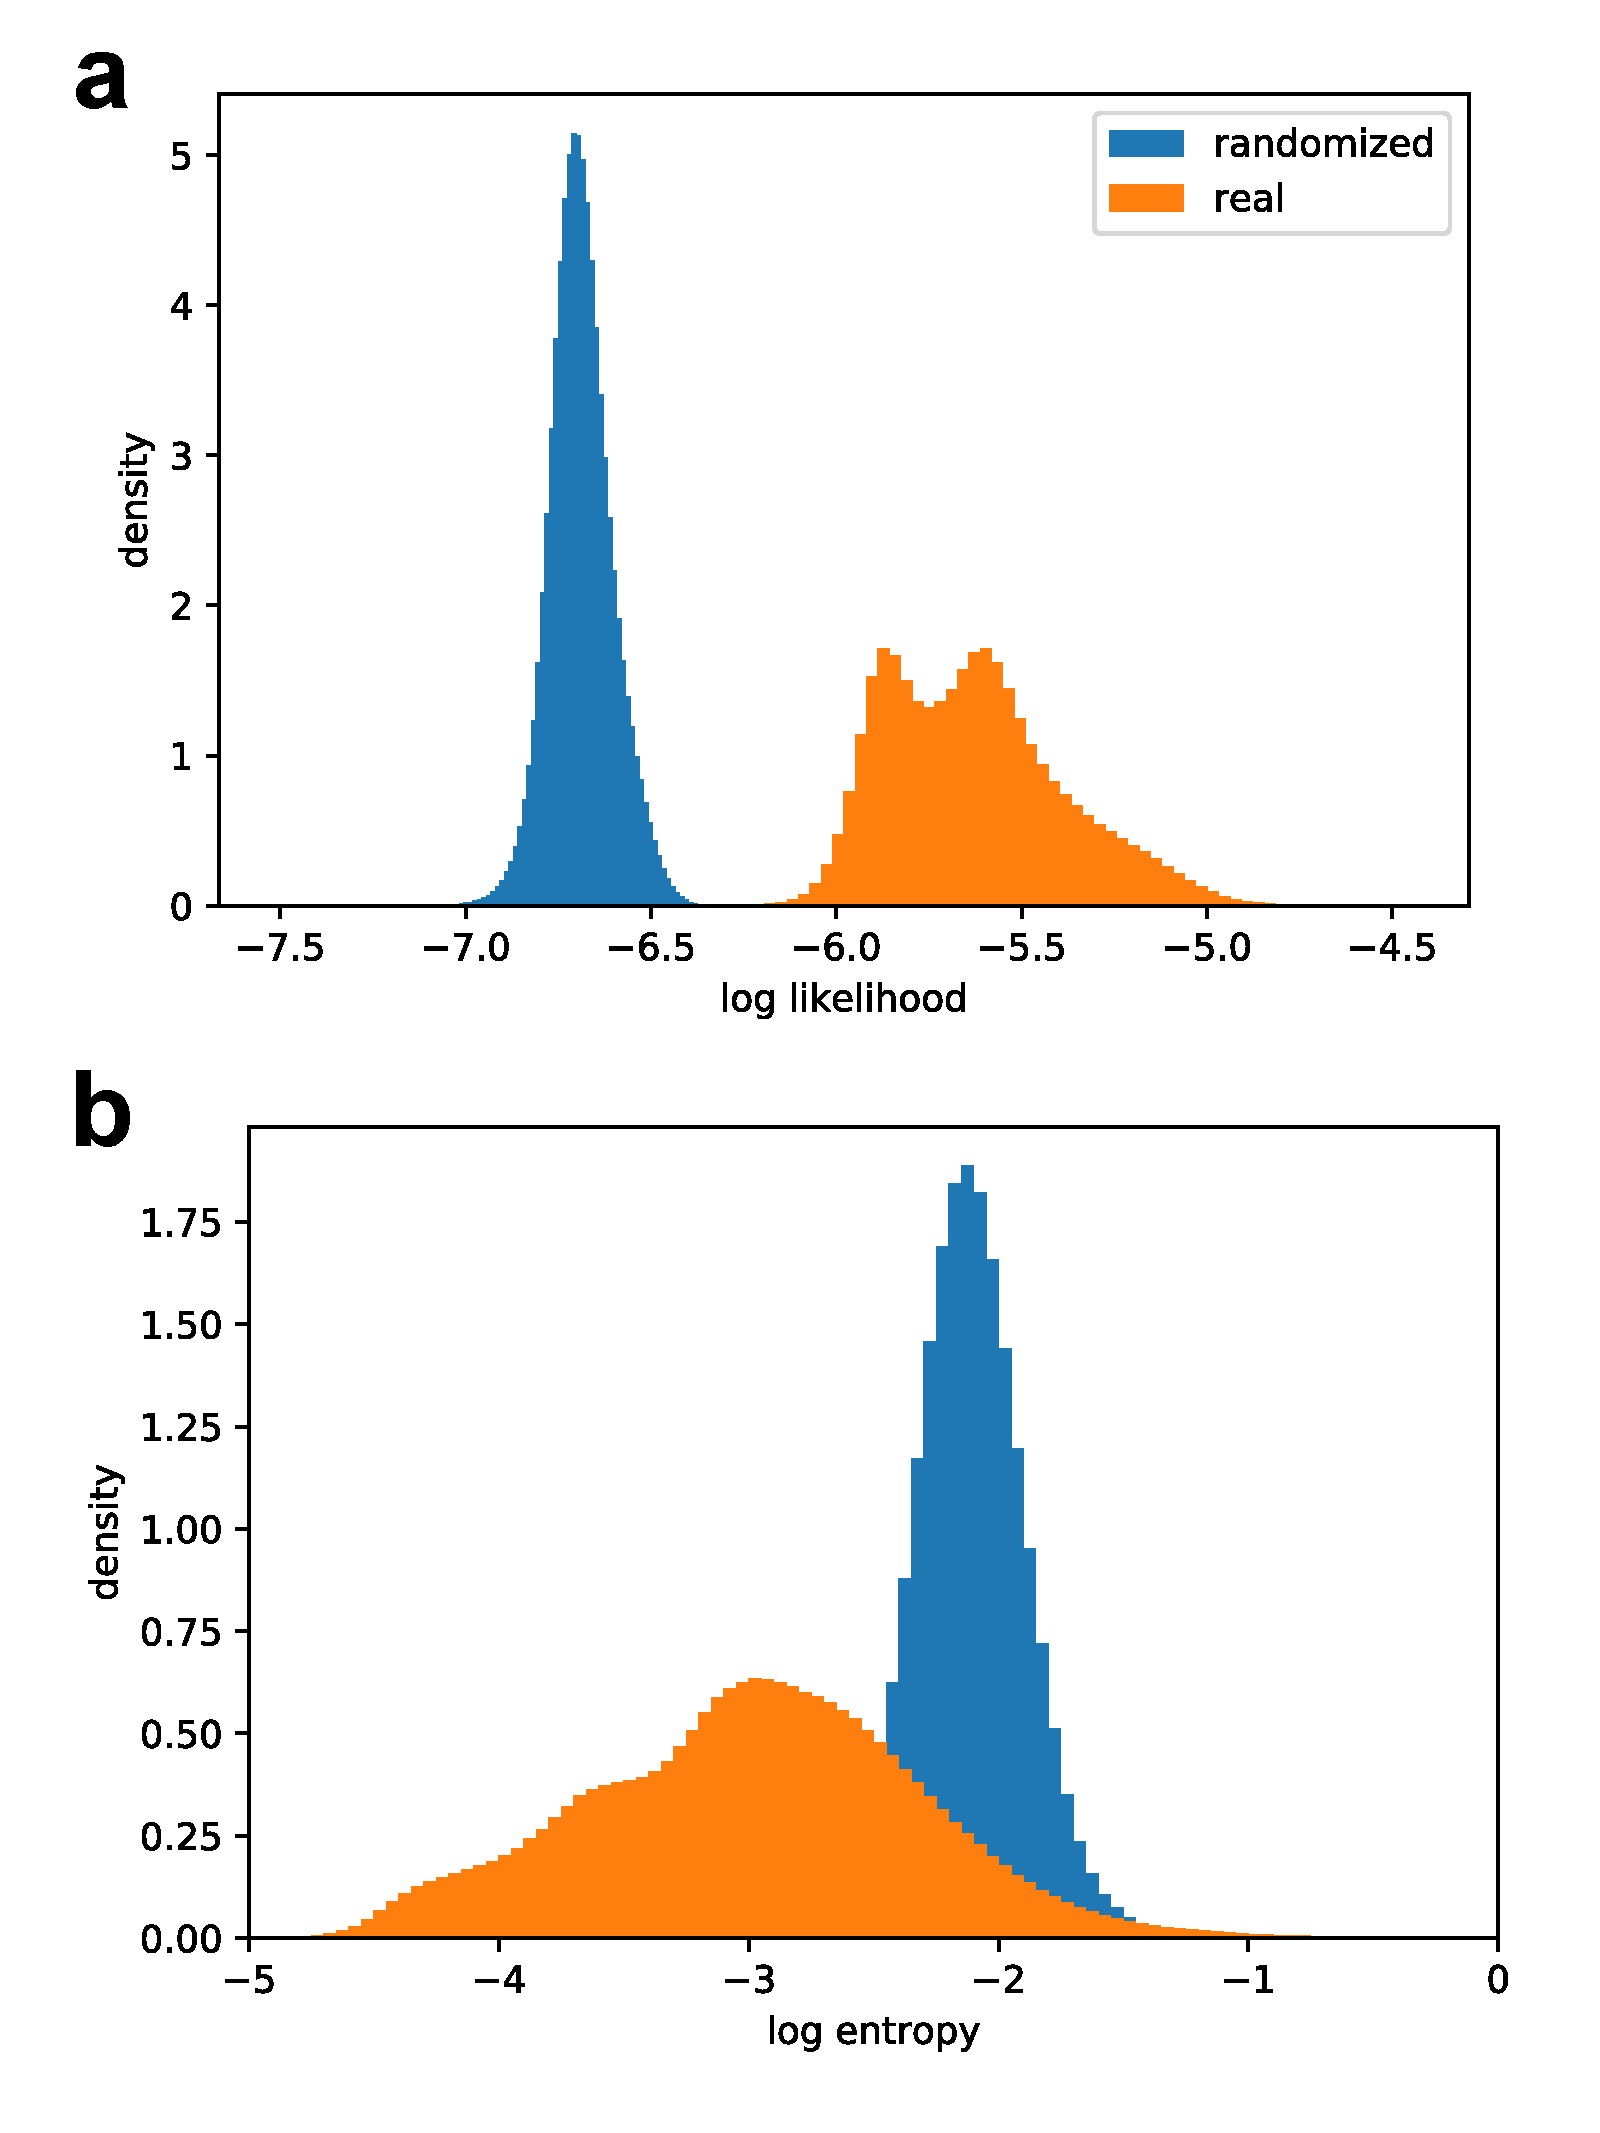
\includegraphics[width=0.5\textwidth]{Graving_IMPRS_Thesis/figures/likelihood_entropy_figure.pdf}
\end{center}

\caption{  \textbf{Likelihood and entropy distributions}. \textbf{a}, Histograms of the log likelihood scores from the decoder (Eq. \ref{eq:elbo}; distortion) for real and randomized data (n = 232,000 for each distribution). \textbf{b}, Histograms of the log entropy from the approximate posterior (Eq. \ref{eq:approx}) for real and randomized data (n = 232,000 for each distribution).}

\label{fig:likelihood_entropy_figure} % \label works only AFTER \caption within figure environment

\end{figure}

\begin{figure}[!htb]
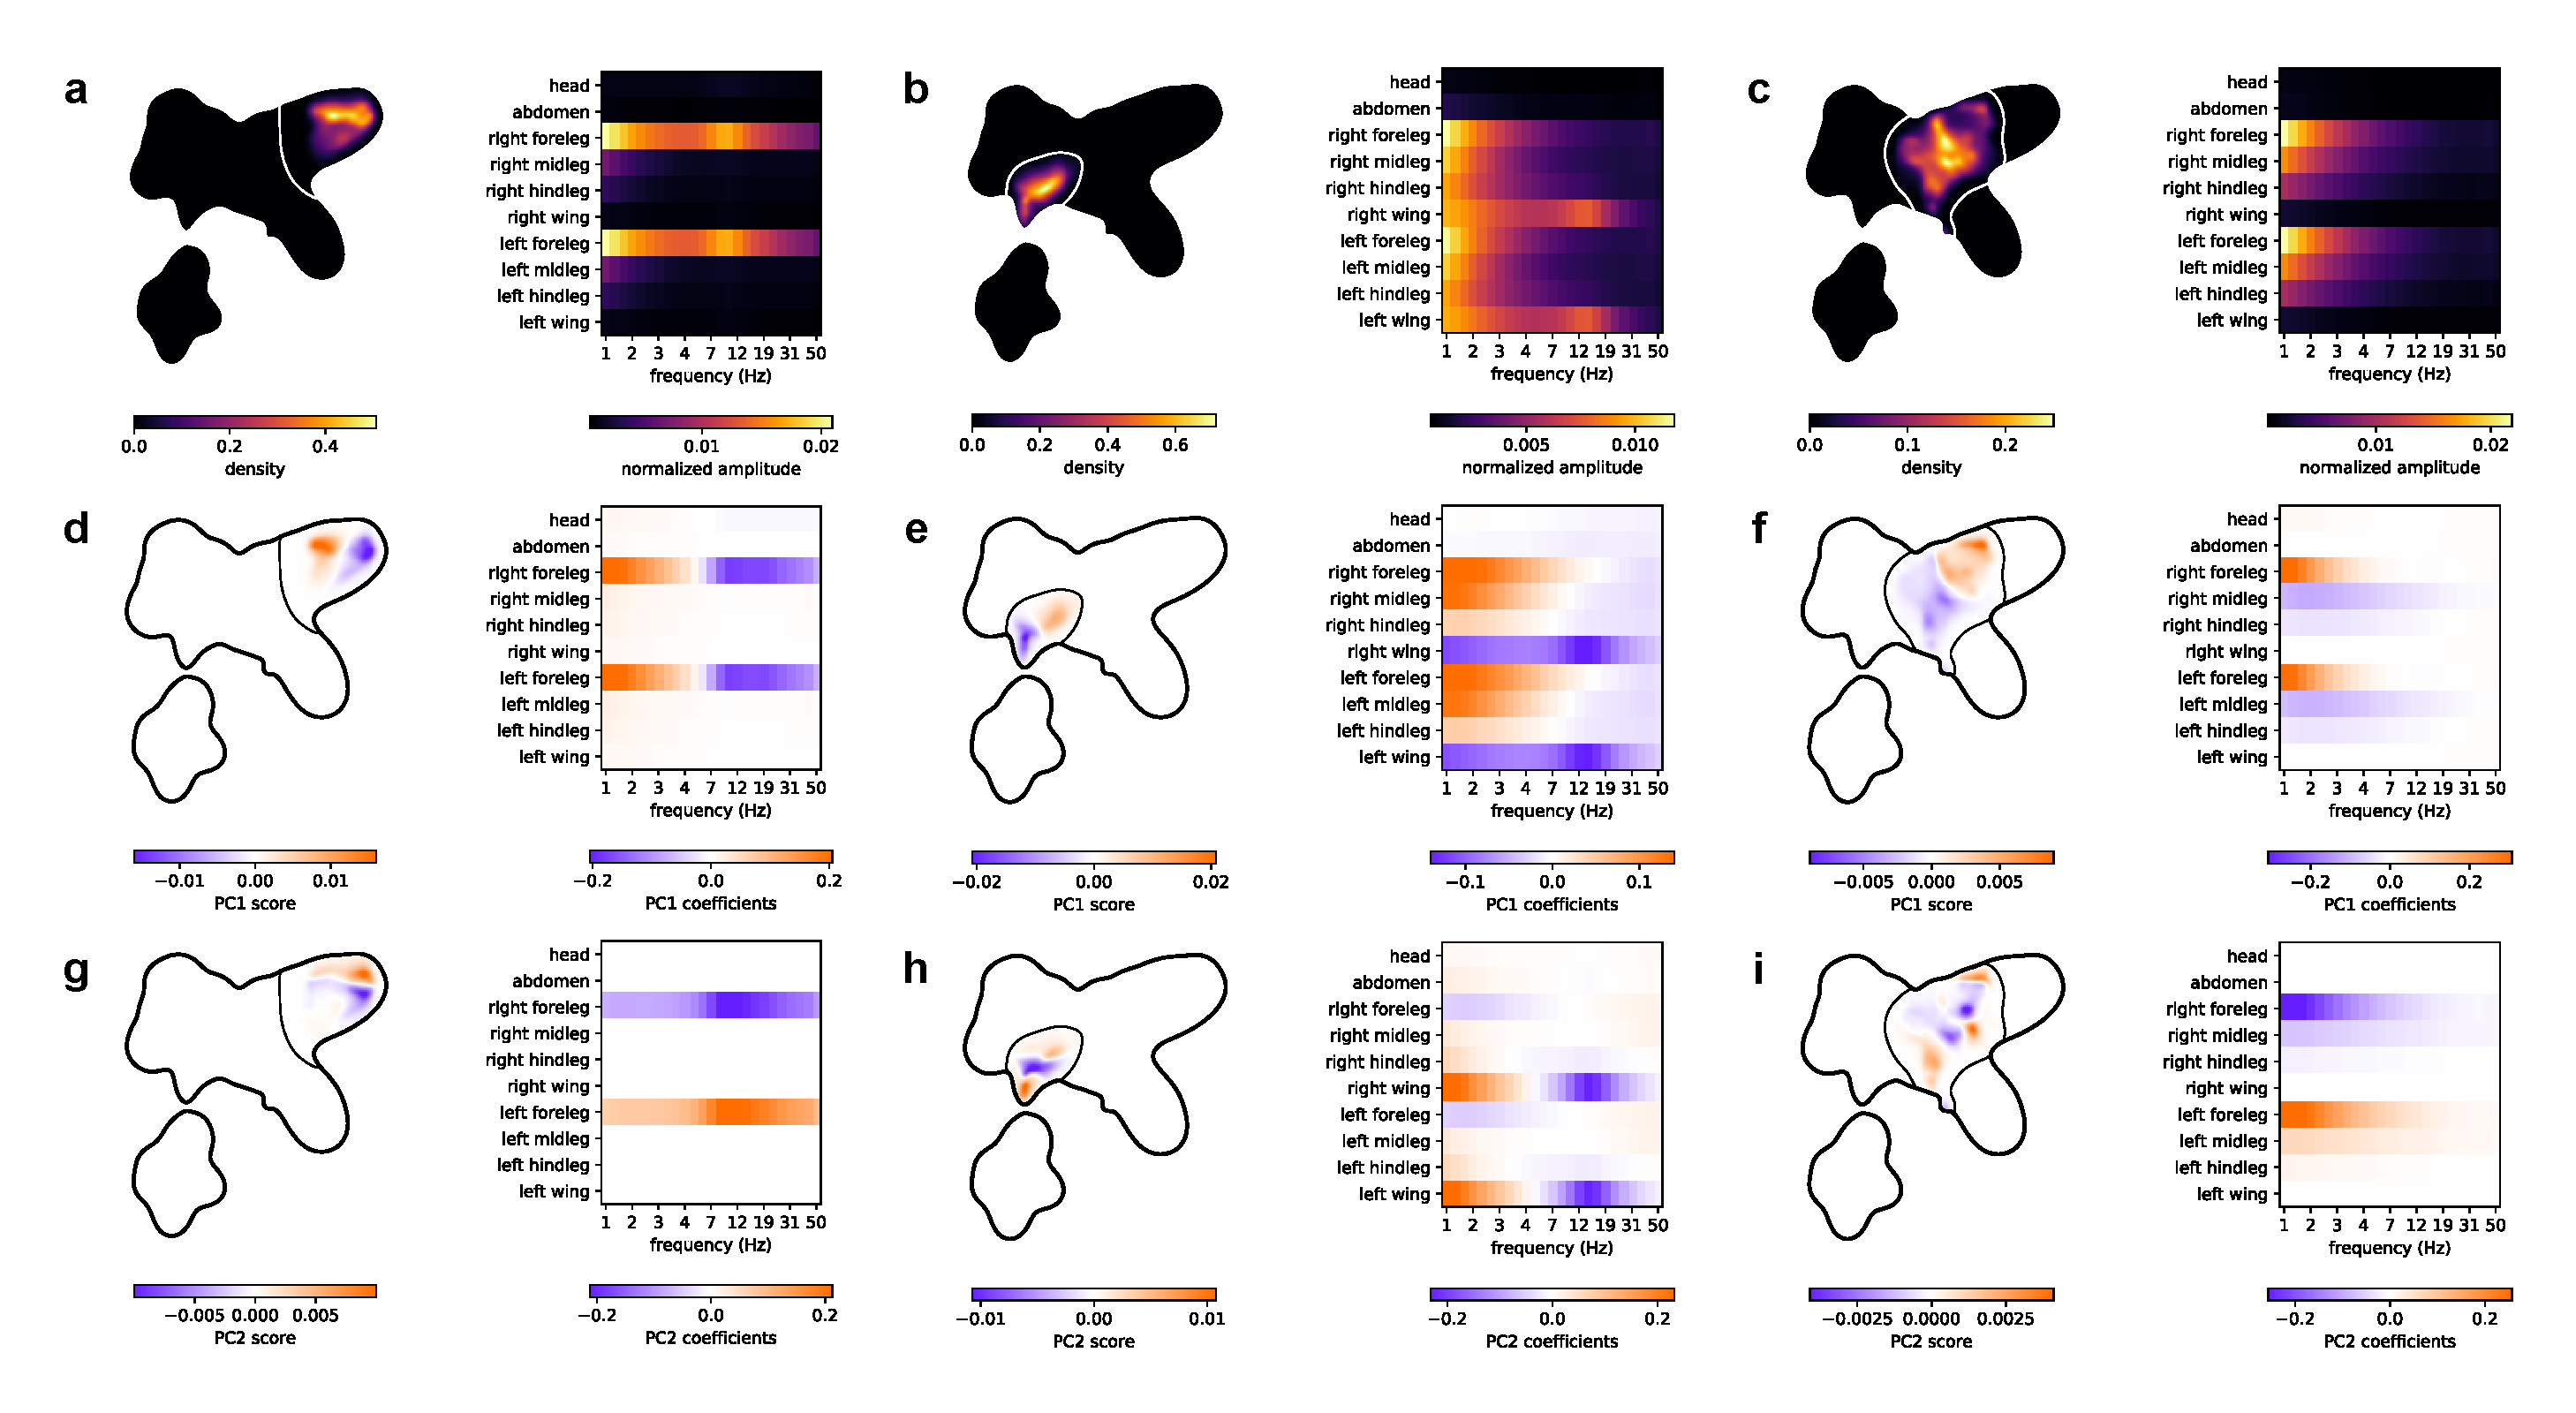
\includegraphics[width=1.0\textwidth]{Graving_IMPRS_Thesis/figures/cluster_appendix.pdf}

\caption{  \textbf{High-level behavioral clusters.} Visualizations describing the manually-grouped high-level clusters for anterior grooming (\textbf{a},\textbf{e},\textbf{g}), wing movements (\textbf{b},\textbf{e},\textbf{h}) and small/slow leg movements (\textbf{c},\textbf{f},\textbf{i}). \textbf{a-c}, The 2-D posterior probability density for each cluster (left), where contours are the largest 90\% probability density contour for each cluster distribution, and the mean spectrogram for each cluster (right). \textbf{d}-\textbf{i}, The principal component scores of the spectrograms assigned to each cluster visualized within the 2-D embedding (left) and the eigenvector coefficients describing the linear contribution of each spectrogram feature (right) for the principal component score.}

\label{fig:cluster_appendix_figure}

\end{figure}

\begin{figure}[!htb]
\centering
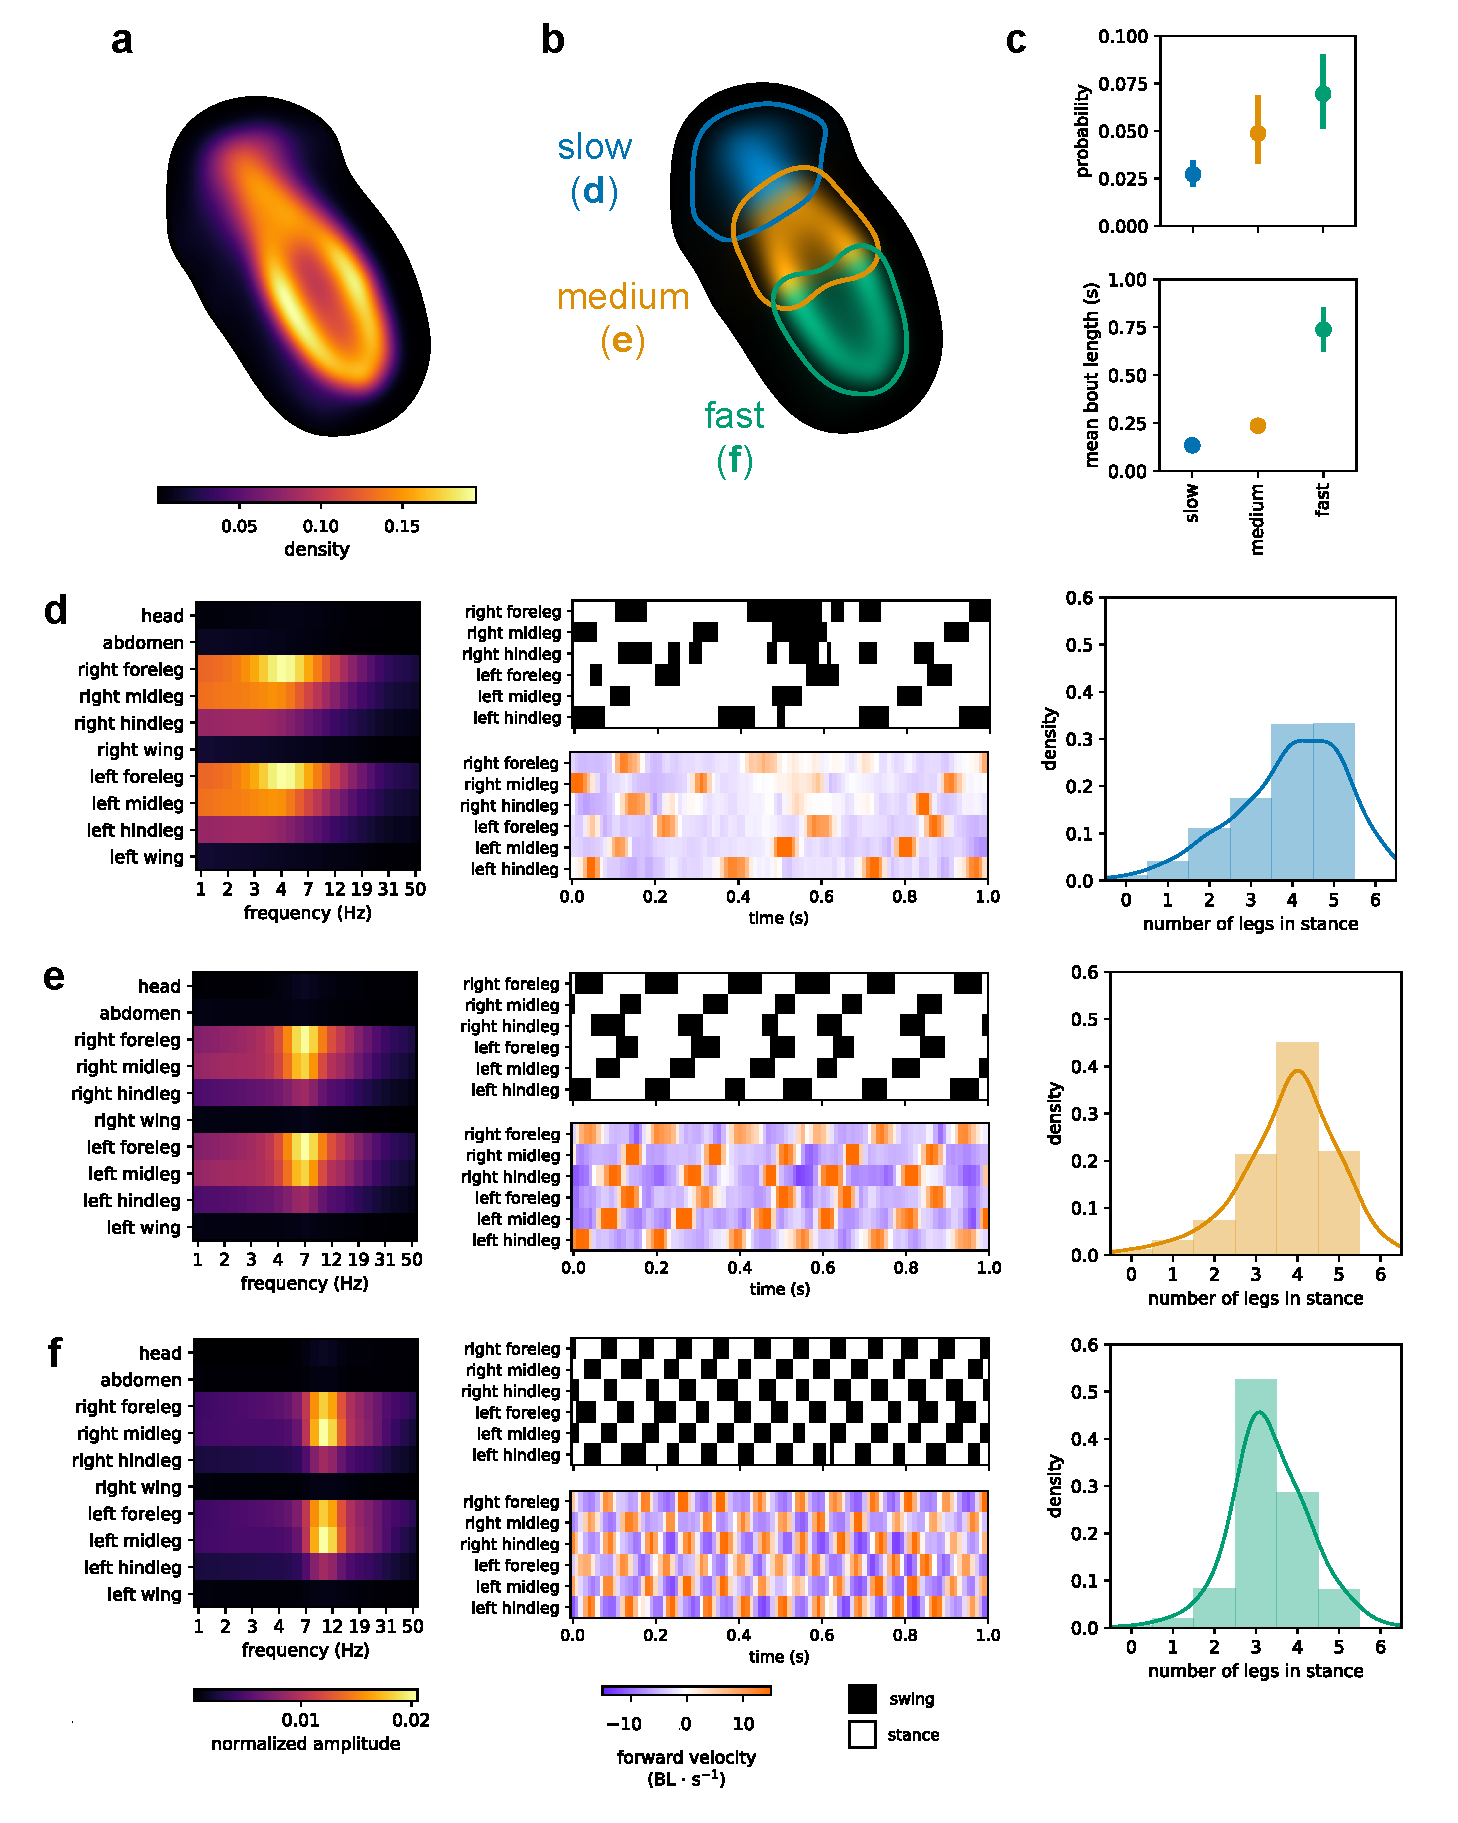
\includegraphics[width=0.9\textwidth]{Graving_IMPRS_Thesis/figures/locomotion_cluster_figure.pdf}
\bigskip
\caption{\textbf{Low-level locomotion clusters.} Visualizations describing the low-level clusters within the high-level locomotion cluster. \textbf{a-b}, The 2-D posterior probability density for the high-level cluster (\textbf{a}) and for each low-level cluster (\textbf{b}), where letters for each cluster label correspond to panels \textbf{d-f}. Contours are the largest 90\% probability density contour for each cluster distribution. \textbf{c}, Mean and 95\% bootstrap intervals of the marginal (stationary) probability and mean bout length for each low-level cluster (n = 59 per cluster). \textbf{d-f}, The mean spectrogram (left), example time segments (middle) showing forward velocity of each leg measured in body lengths (BL) per second and swing (forward velocity $> 0 \, \textrm{BL} \cdot \textrm{s}^{-1}$) or stance (forward velocity $\leq 0 \, \textrm{BL} \cdot \textrm{s}^{-1}$) classification, and histograms (right) showing the number of legs classified as stance in each timestep assigned to each cluster (n = 0.57 million for slow, \textbf{d}; n = 1.03 million for medium, \textbf{e}; and n = 1.47 million for fast, \textbf{f}) --- where the label for each panel in \textbf{d-f} corresponds to a cluster label in panel \textbf{b}. Example videos for these low-level clusters are shown in \ref{fig:locomotion_video}.}

\label{fig:locomotion_cluster_figure}

\end{figure}

\begin{figure}[!htb]
\centering
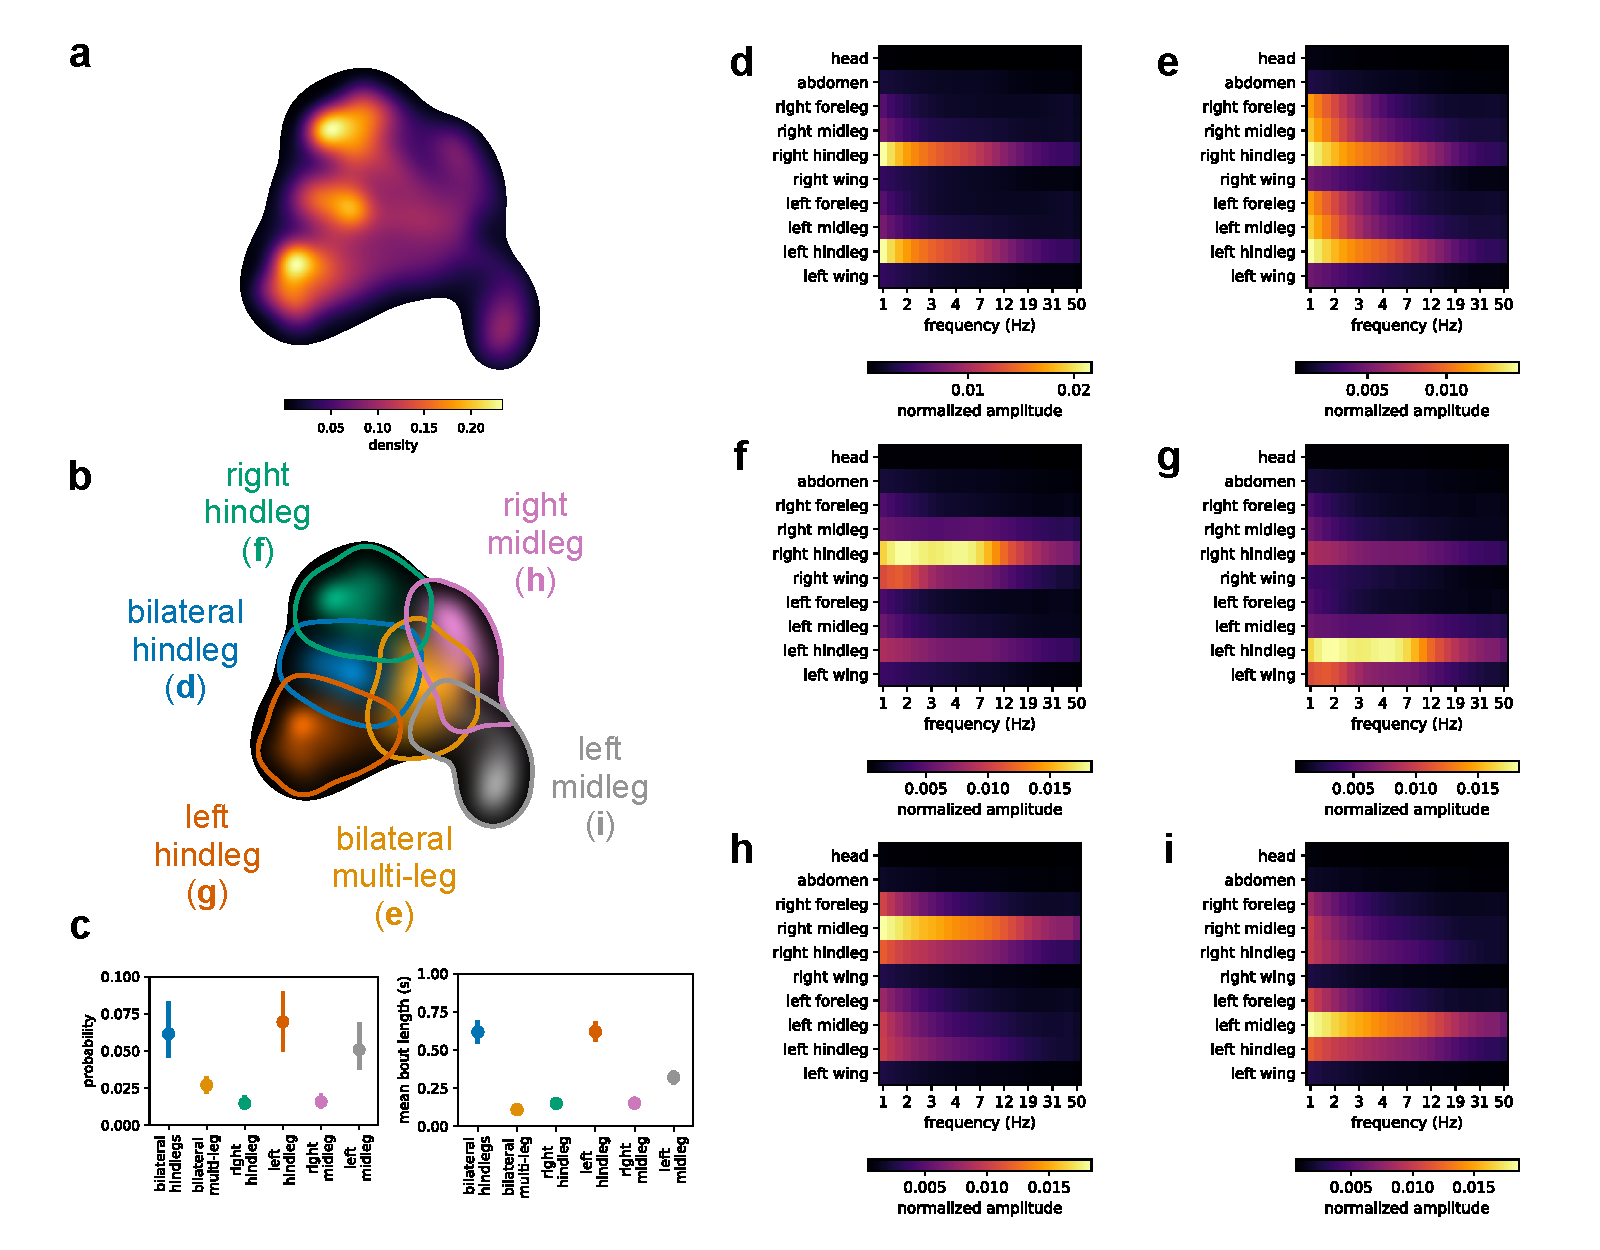
\includegraphics[width=1.0\textwidth]{Graving_IMPRS_Thesis/figures/posterior_cluster_figure.pdf}

\caption{  \textbf{Low-level posterior grooming clusters.} Visualizations describing the low-level clusters within the high-level posterior grooming cluster. \textbf{a-b}, The 2-D posterior probability density for the high-level cluster (\textbf{a}) and for each low-level cluster (\textbf{b}), where letters for each cluster label correspond to panels \textbf{d-i}. Contours are the largest 90\% probability density contour for each cluster distribution. \textbf{c}, Mean and 95\% bootstrap intervals of the marginal (stationary) probability and mean bout length for each low-level cluster (n = 59 per cluster). \textbf{d-i}, The mean spectrogram for each cluster --- where the label for each panel in \textbf{d-i} corresponds to a cluster label in panel \textbf{b}. Example videos for these low-level clusters are shown in \ref{fig:posterior_video}.}

\label{fig:posterior_cluster_figure}

\end{figure}


\begin{figure}[!htb]
\begin{center}
    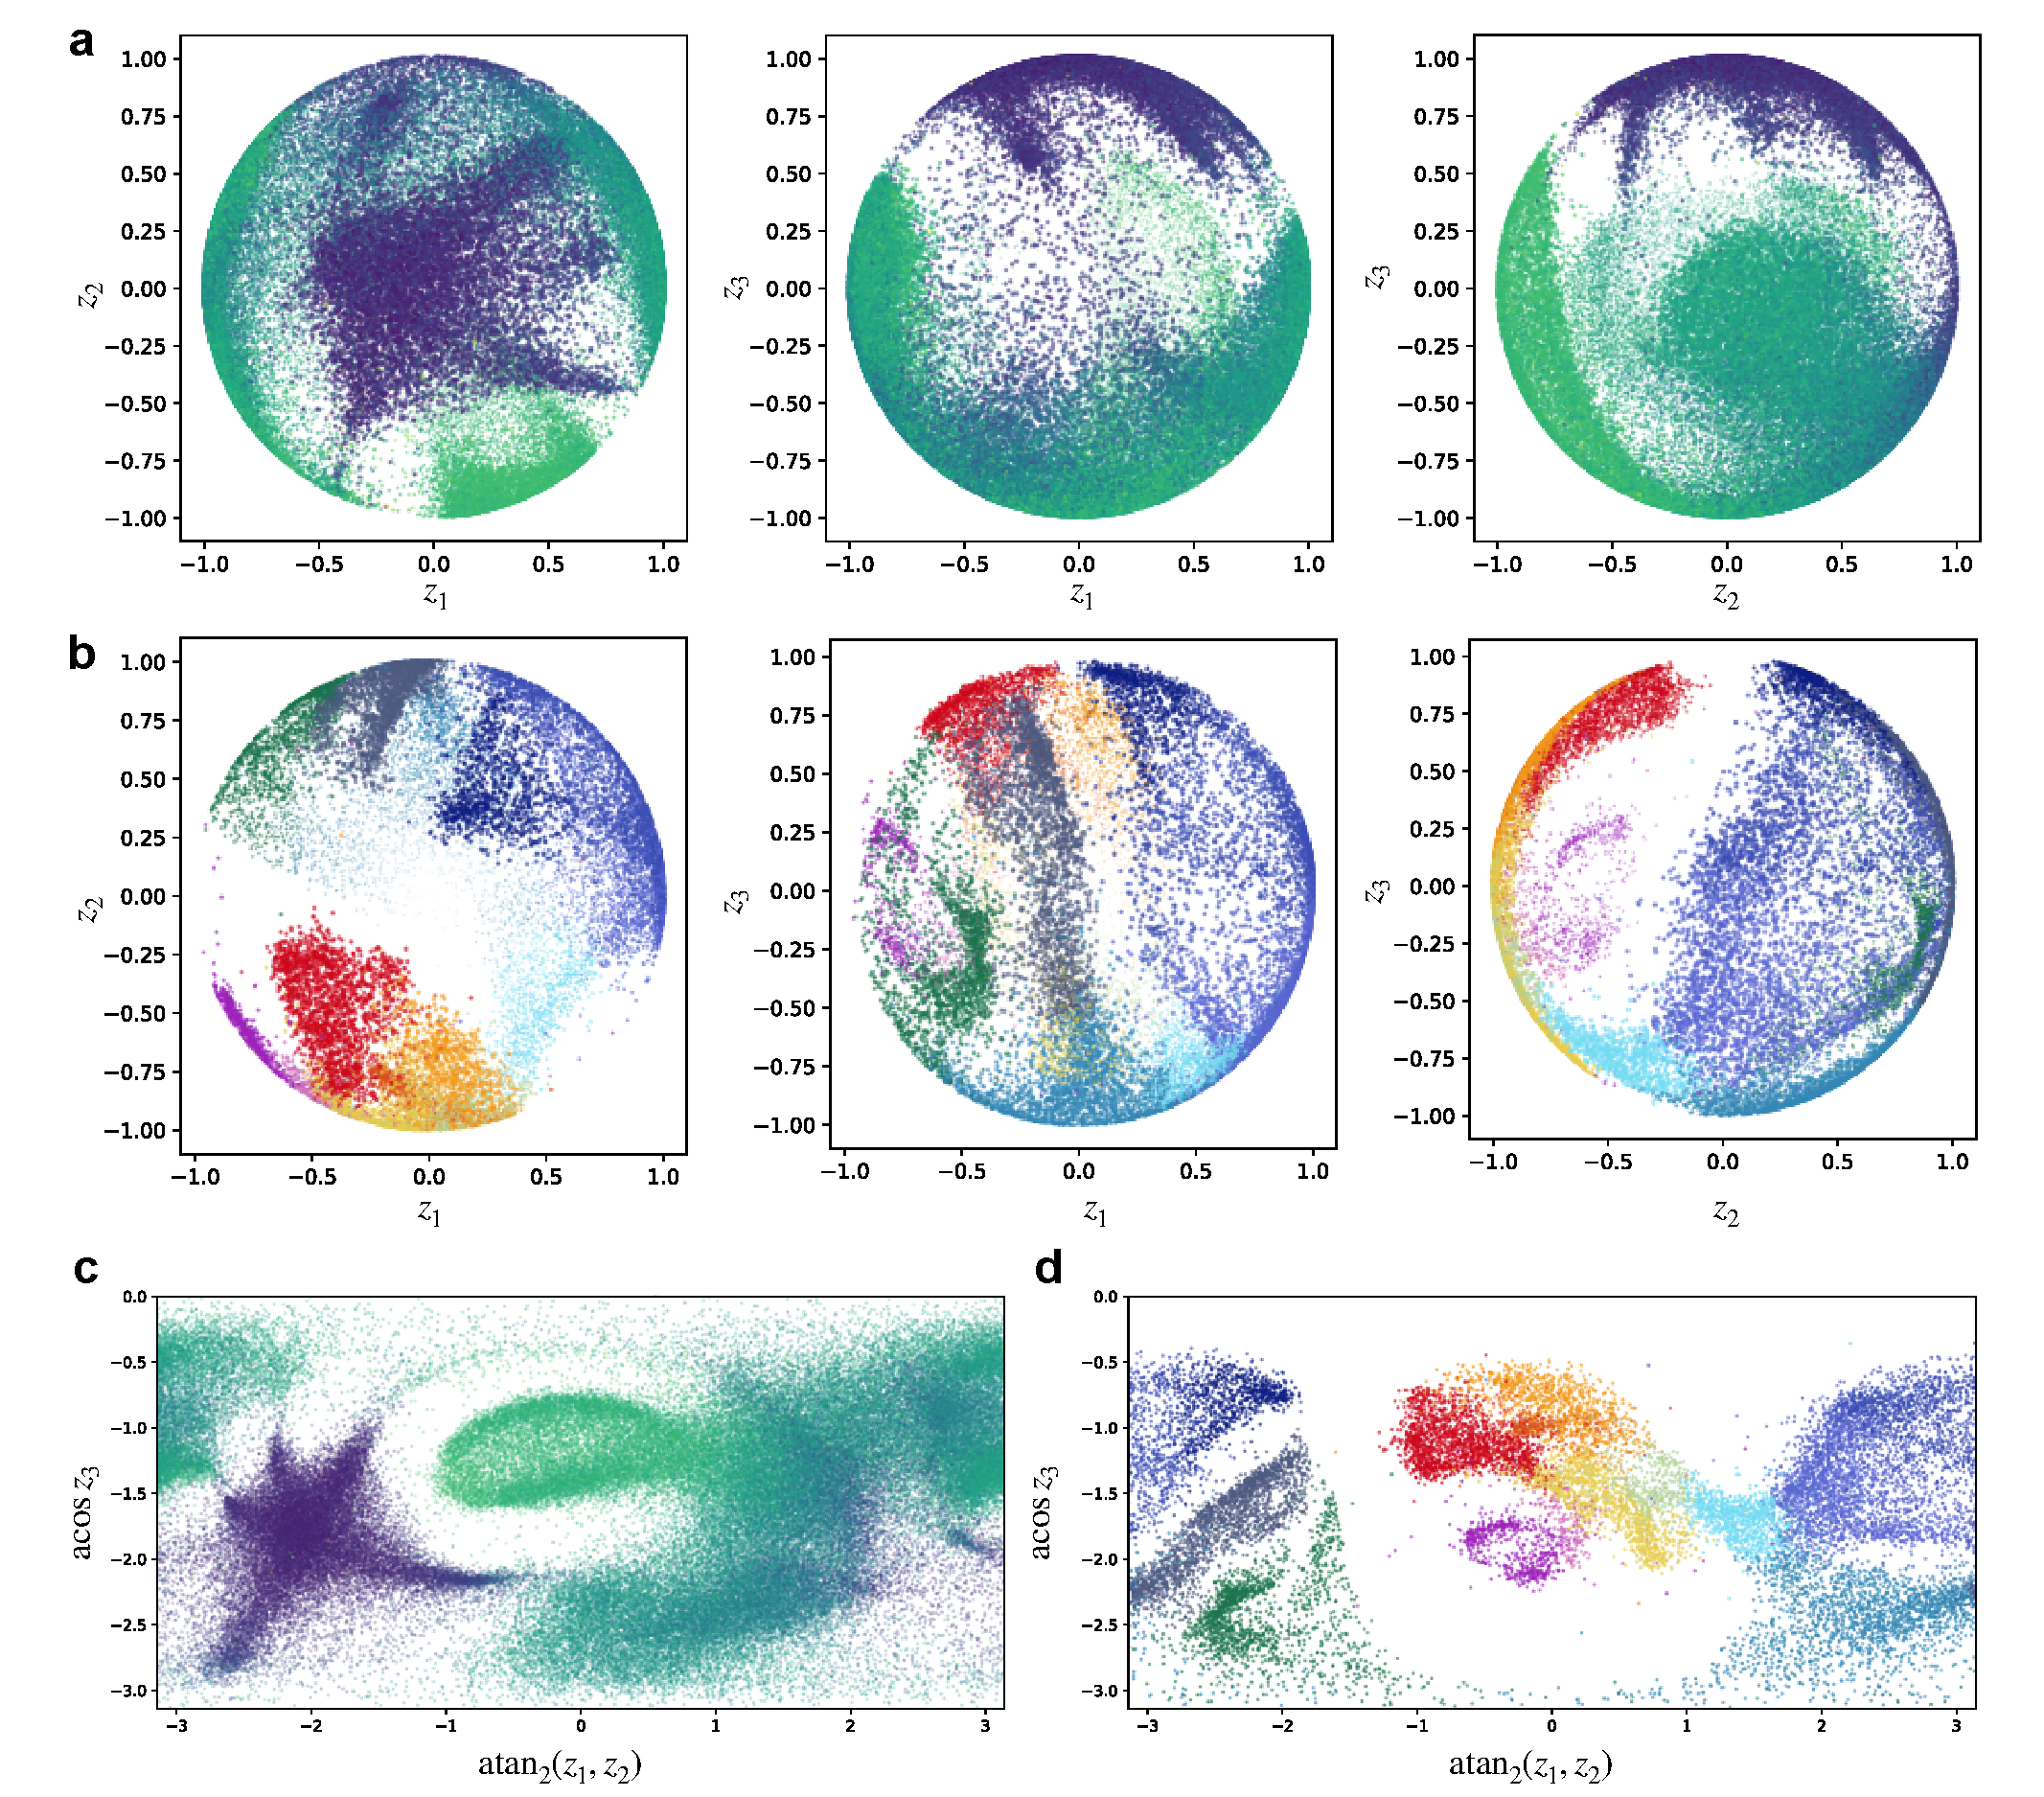
\includegraphics[width=\textwidth]{Graving_IMPRS_Thesis/figures/spherical_figure.pdf}
\end{center}

\caption{  \textbf{Spherical embeddings with von Mises-Fisher VAE-SNE}. \textbf{a-b}, Spherical embeddings using VAE-SNE with a von Mises-Fisher similarity kernel (Appendix \ref{appendix:spherical}) of the posture dynamics dataset (\textbf{a}; \ref{fig:spherical_embedding_posture_video}) from \cite{berman2014mapping, berman2016predictability, pereira2019fast} and the single-cell RNA-seq dataset (\textbf{b}; \ref{fig:spherical_embedding_rna_video}) from \cite{la2018rna}. \textbf{c-d}, Stereographic (planar) projections of the spherical embeddings from \textbf{a-b}. Colors for \textbf{a-d} are the same as in Fig. \ref{fig:embedded_data_figure} (total amplitude and cell type).}

\label{fig:spherical_figure} % \label works only AFTER \caption within figure environment

\end{figure}


\begin{figure}[!htb]
\begin{center}
    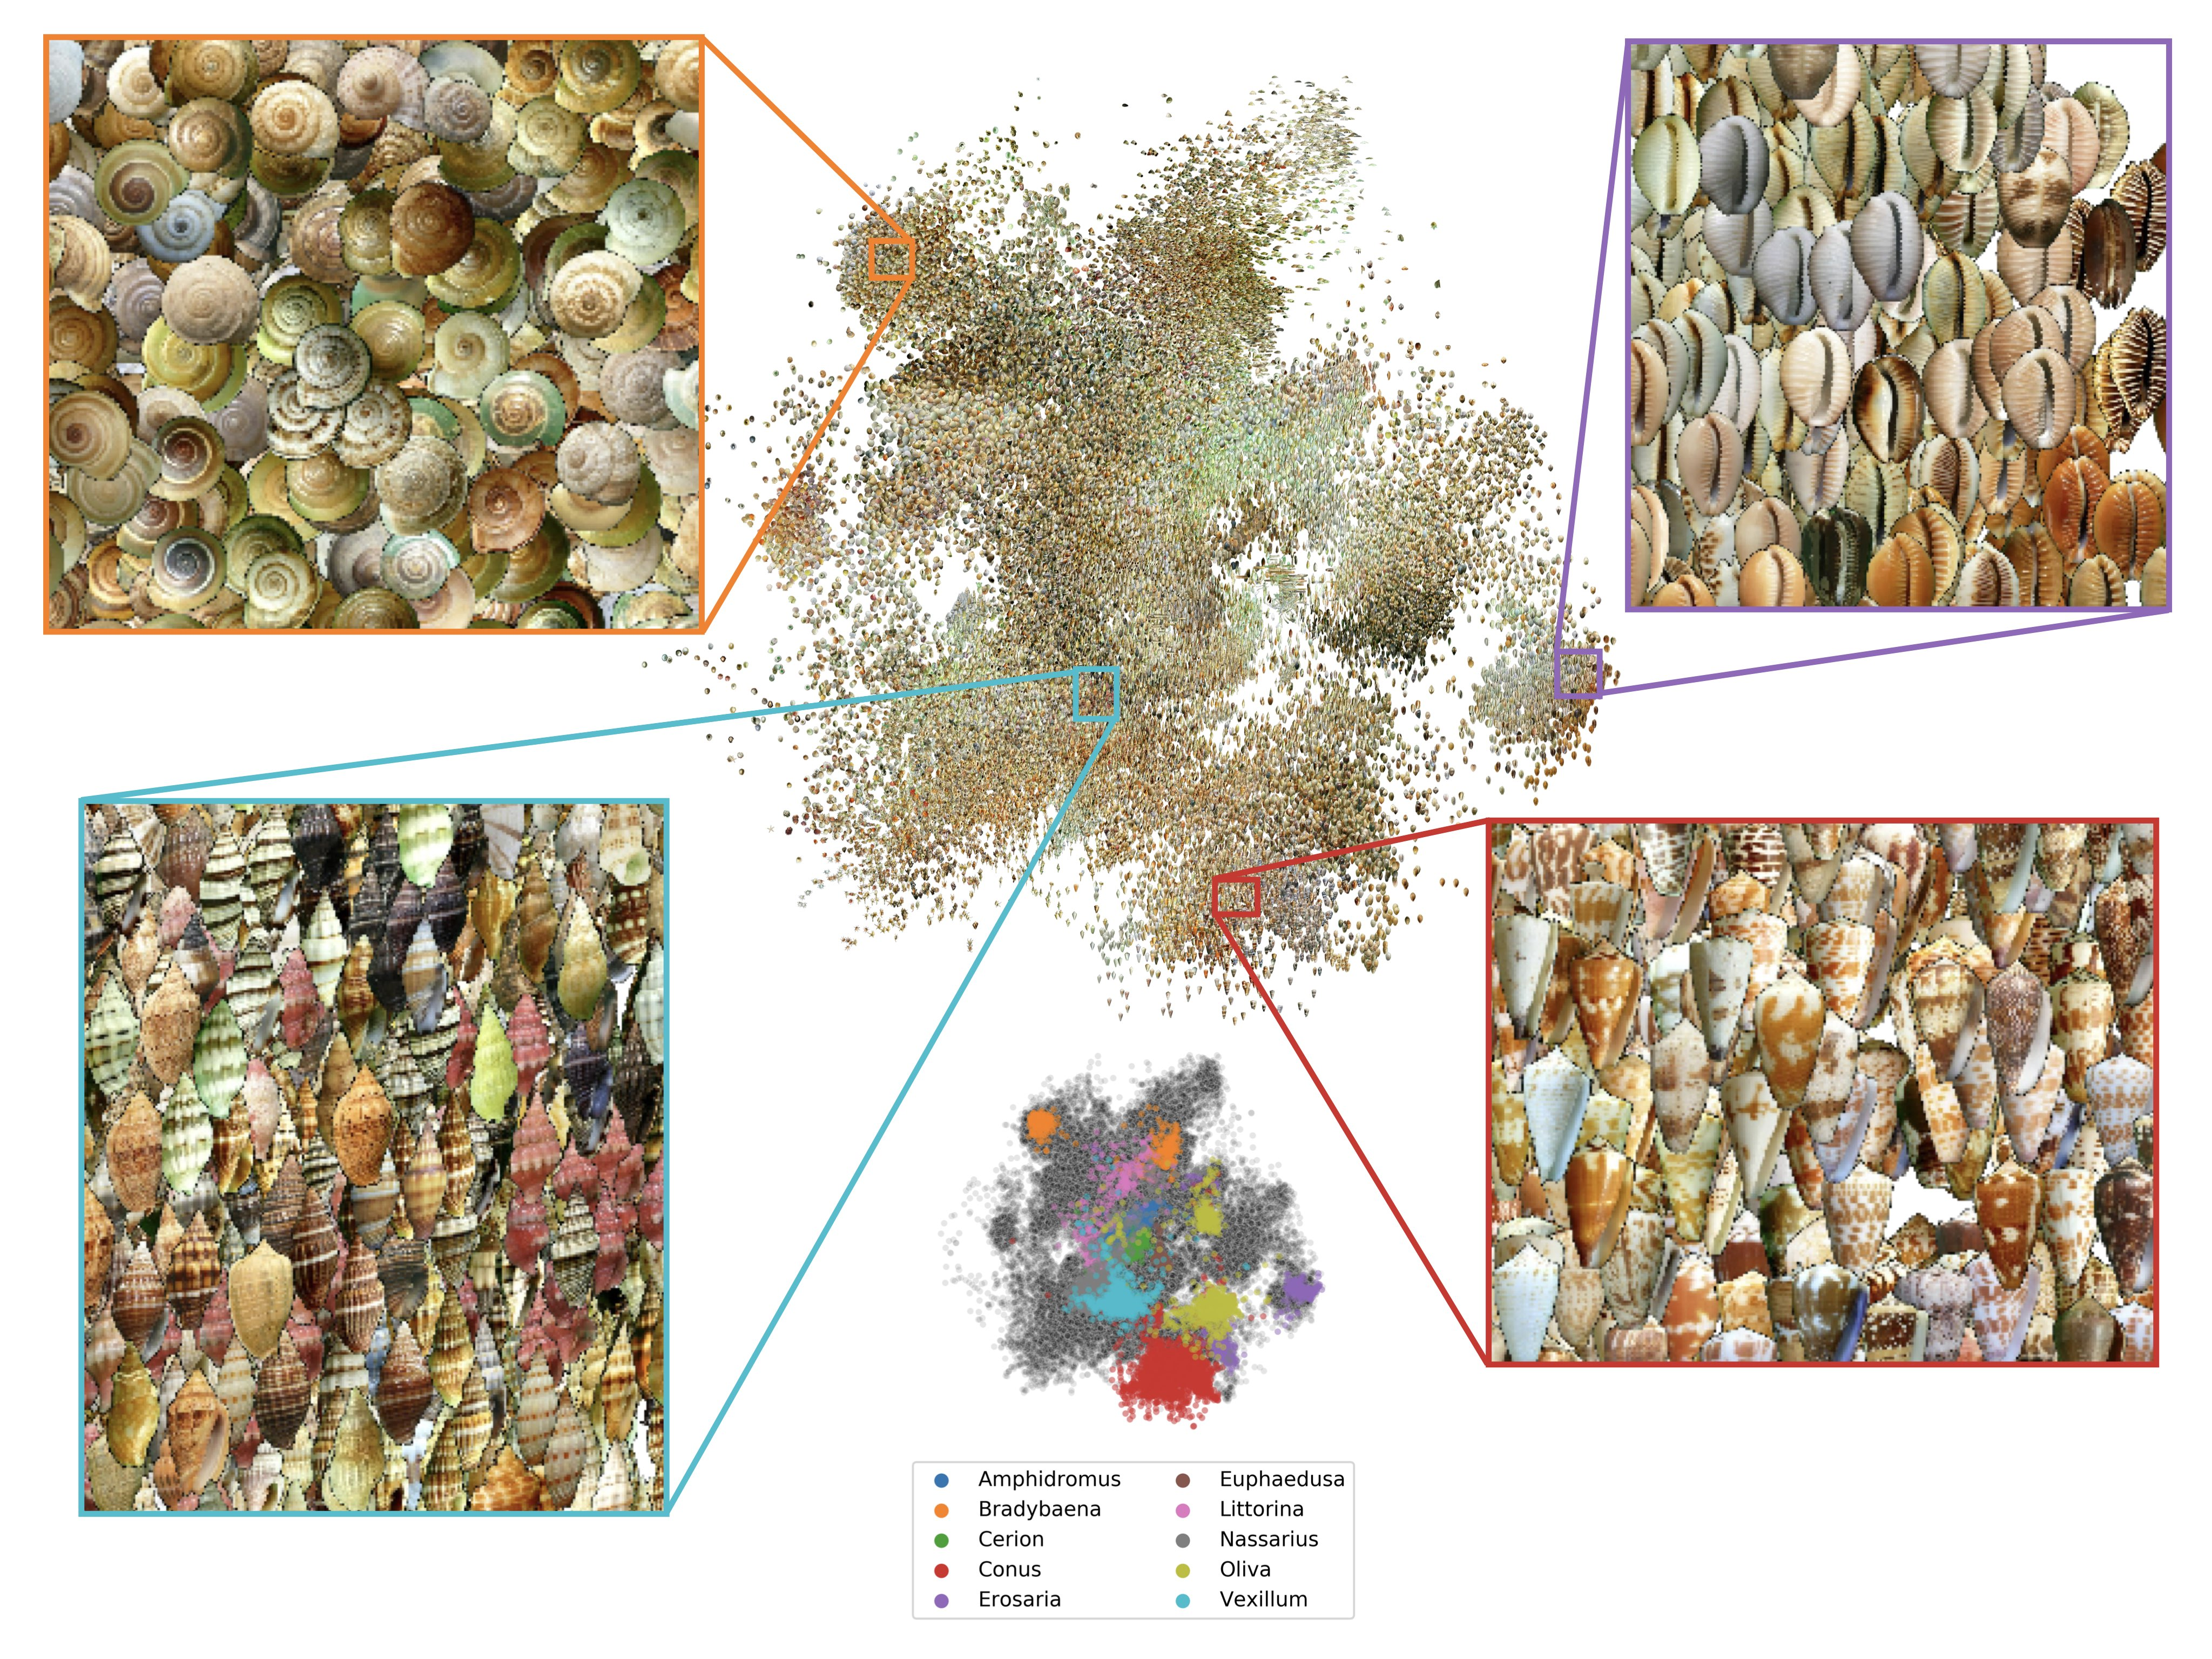
\includegraphics[width=\textwidth]{Graving_IMPRS_Thesis/figures/shell_figure.jpeg}
\end{center}

\caption{  \textbf{Embedding shell images}. Shell images from \cite{zhang2019shell} embedded in two dimensions using convolutional VAE-SNE. Insets illustrate example regions of perceptually similar images from the taxonomic genera \textit{Bradybaena} (land snails; top-left), \textit{Erosaria} (cowries; top-right), \textit{Vexillum} (sea snails; bottom-left), and \textit{Conus} (cone snails; bottom-right). Scatter plot (bottom-center) shows the 10 most common genera in the dataset.}

\label{fig:shell_figure} % \label works only AFTER \caption within figure environment

\end{figure}

\begin{figure}[!htb]
\begin{center}
    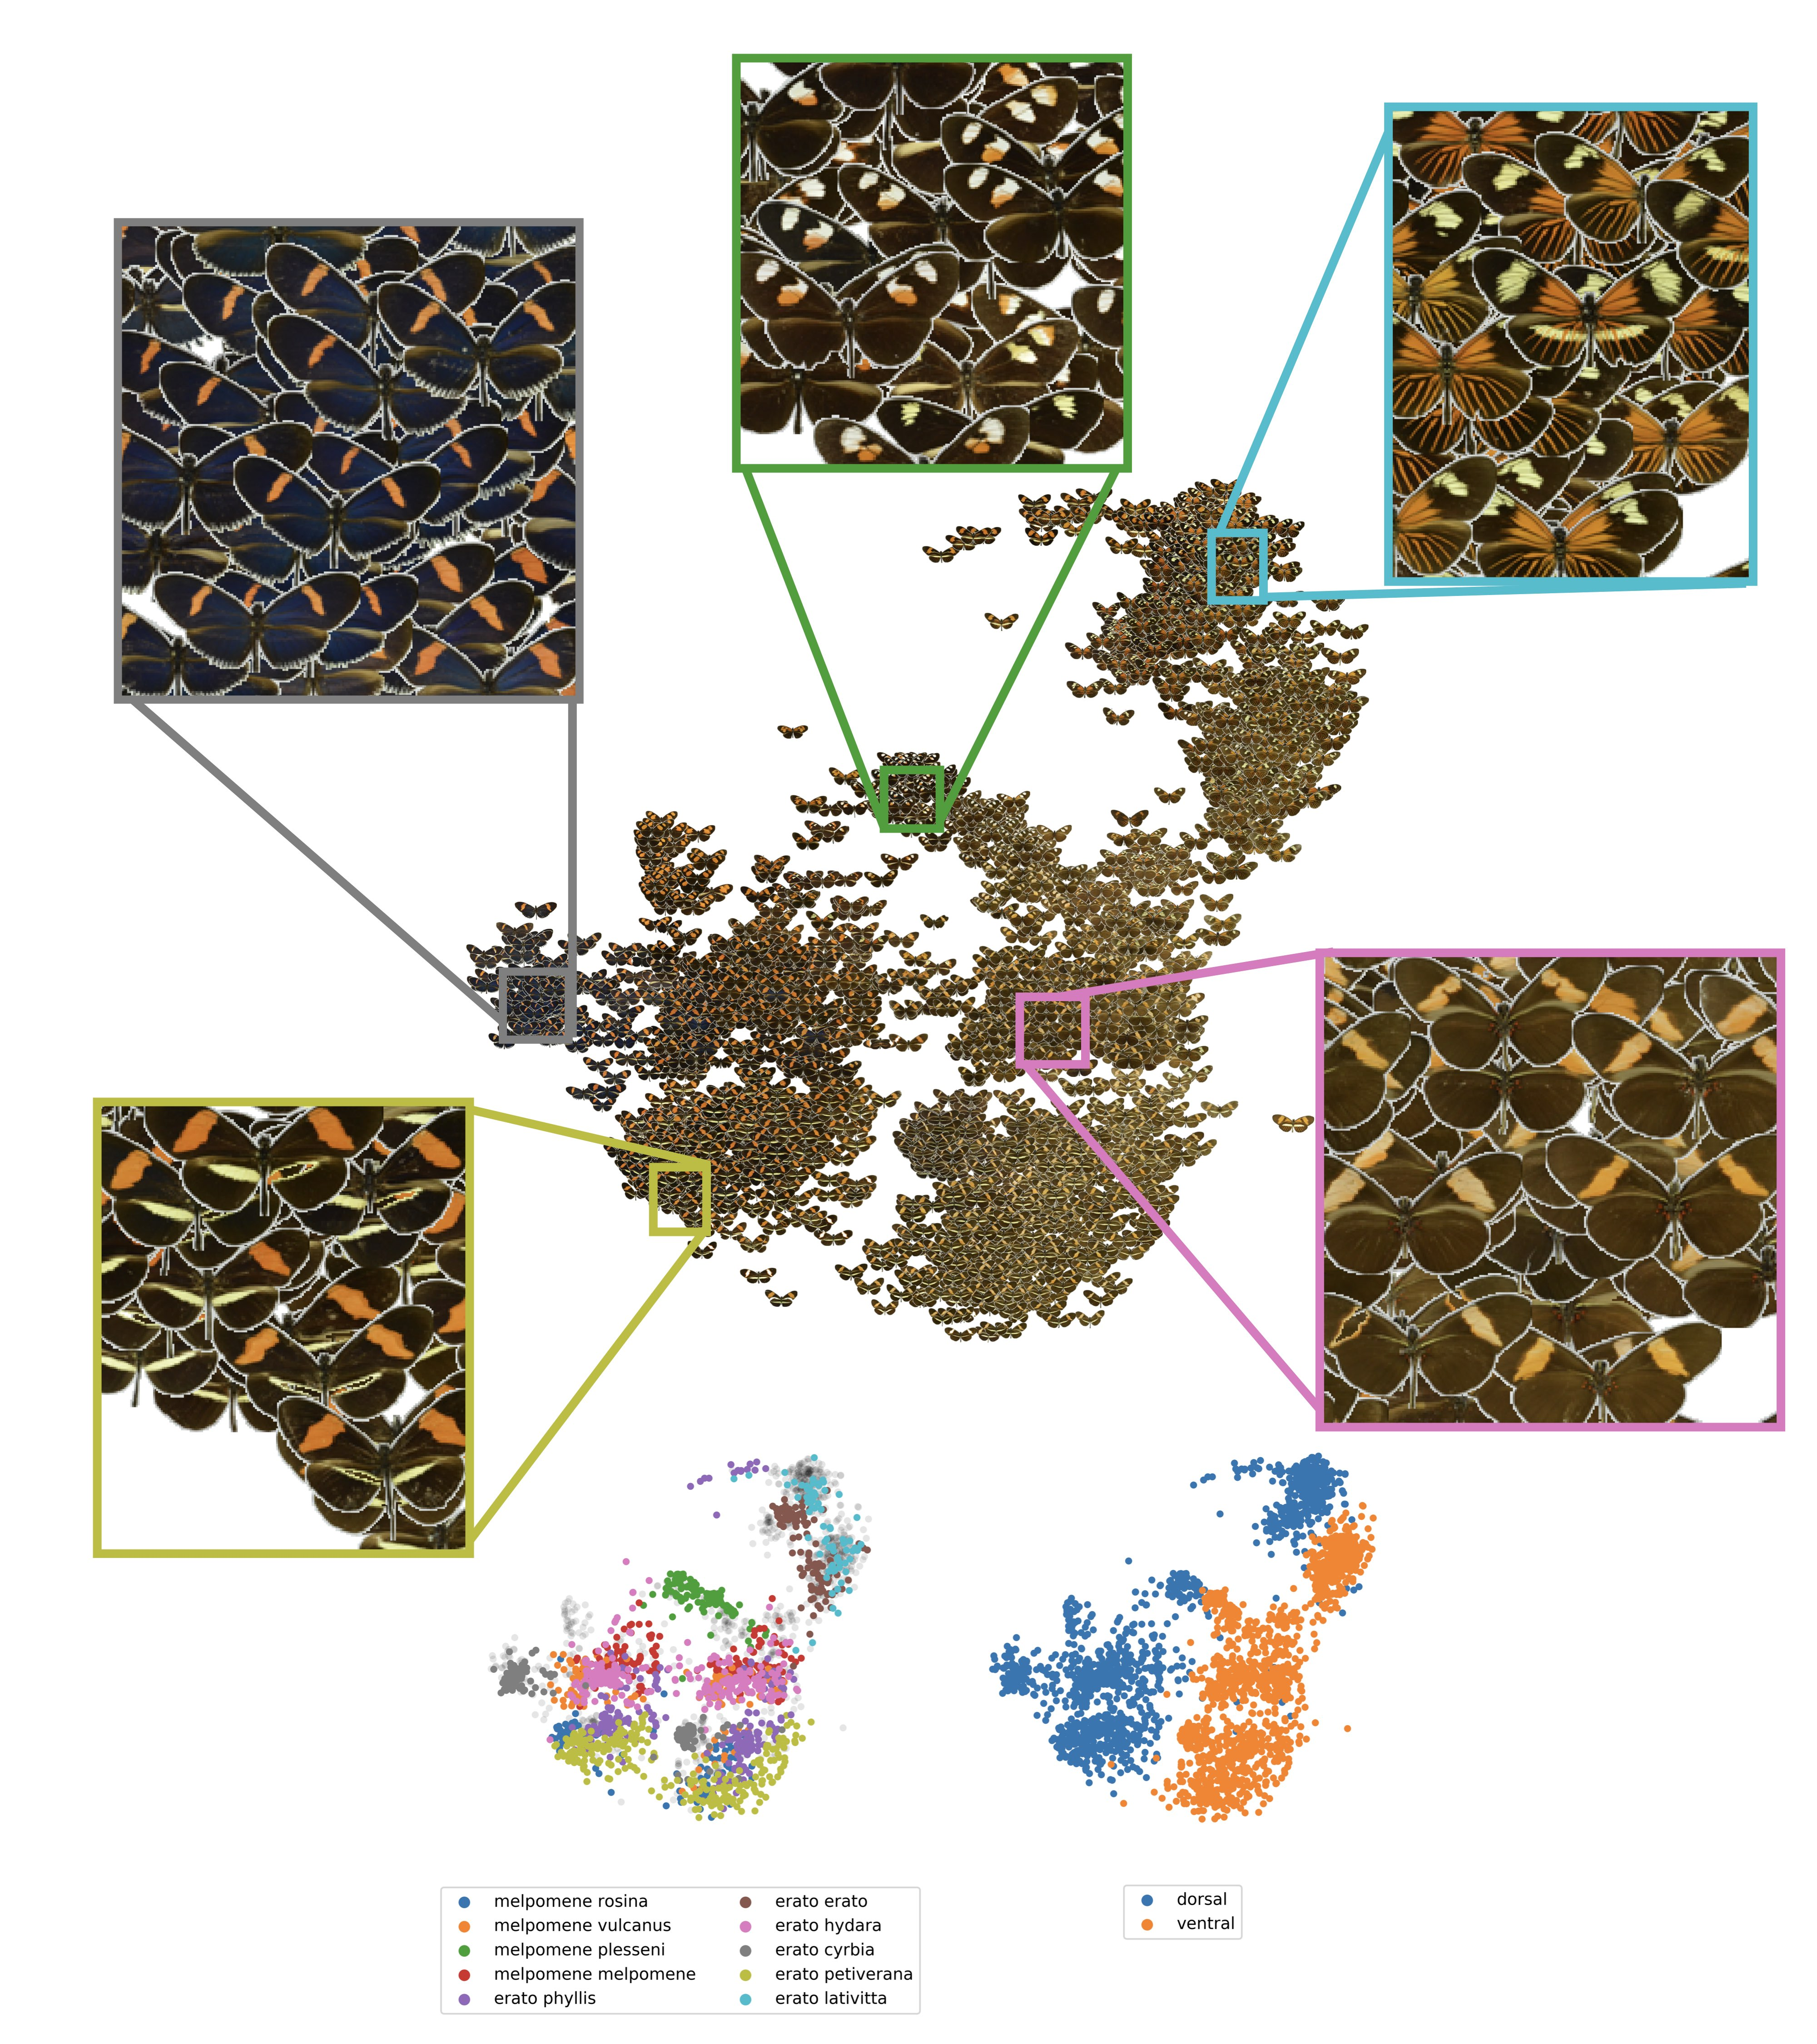
\includegraphics[width=\textwidth]{Graving_IMPRS_Thesis/figures/butterfly_figure.jpeg}
\end{center}

\caption{  \textbf{Embedding butterfly images}. Butterfly (\textit{Heliconius spp.}) images from \cite{cuthill2019deep} embedded in two dimensions using convolutional VAE-SNE. Insets show example regions of perceptually similar subspecies (top). Scatter plots (bottom) show labels for the 10 most common subspecies in the dataset (bottom-left) and the image viewpoint relative to the specimen's dorso-ventral body axis (bottom-right).}

\label{fig:butterfly_figure} % \label works only AFTER \caption within figure environment

\end{figure}

\clearpage
\setcounter{figure}{0}
\renewcommand{\thefigure}{Video S\arabic{figure}}

\begin{figure}[!htb]
\caption{
\textbf{Video segments labeled with VAE-SNE}. Randomly selected video segments ($1/2 \times$ speed) labeled with VAE-SNE illustrating the temporal dynamics of movements through the behavioral space and transitions between high-level clusters within the distribution. \textbf{a}, \href{https://youtu.be/JlbSdKzvLfk}{https://youtu.be/JlbSdKzvLfk}; \textbf{b}, \href{https://youtu.be/uWScG_UuzRQ}{https://youtu.be/uWScG\_UuzRQ}; \textbf{c}, \href{https://youtu.be/T8e_JSoCwMA}{https://youtu.be/T8e\_JSoCwMA}
}
\label{fig:sequences_video}
\end{figure}


\begin{figure}[!htb]
\caption{
\textbf{Samples from the locomotion cluster}. Randomly sampled videos ($1/3 \times$ speed) from the locomotion cluster showing: \textbf{a}, slow walking (\href{https://youtu.be/hB3JIRF2JGQ}{https://youtu.be/hB3JIRF2JGQ}); \textbf{b}, medium walking (\href{https://youtu.be/kNHGJypOGhs}{https://youtu.be/kNHGJypOGhs}); and \textbf{c}, fast walking (\href{https://youtu.be/A2sLtgYhHGc}{https://youtu.be/A2sLtgYhHGc}). Red lines show the posture tracking data for all 32 keypoints.
}
\label{fig:locomotion_video}
\end{figure}

\begin{figure}[!htb]
\caption{
\textbf{Samples from the anterior grooming cluster}. Randomly sampled videos ($1/3 \times$ speed) from one of the anterior grooming clusters (\href{https://youtu.be/0MT3lb2bJro}{https://youtu.be/0MT3lb2bJro}). Red lines show the posture tracking data for all 32 keypoints.
}
\label{fig:anterior_video}
\end{figure}

\begin{figure}[!htb]
\caption{
\textbf{Samples from the posterior grooming cluster}. Randomly sampled videos ($1/3 \times$ speed) from the posterior grooming cluster showing: \textbf{a}, bilateral hindleg grooming (\href{https://youtu.be/O_Tyf4pEQMo}{https://youtu.be/O\_Tyf4pEQMo}); \textbf{b}, right hindleg grooming (\href{https://youtu.be/VTIwZp6d6b4}{https://youtu.be/VTIwZp6d6b4}); \textbf{b}, left midleg grooming (\href{https://youtu.be/0vJvAINbfjw}{https://youtu.be/0vJvAINbfjw}). Red lines show the posture tracking data for all 32 keypoints. 
}
\label{fig:posterior_video}

\end{figure}

\begin{figure}[!htb]
\caption{
\textbf{Samples from the wing movements cluster}. Randomly sampled videos ($1/3 \times$ speed) from the wing movements cluster showing: \textbf{a}, wing extensions (\href{https://youtu.be/lE31SeJ7ehY}{https://youtu.be/lE31SeJ7ehY}); and \textbf{b}, wing flicks (\href{https://youtu.be/nsgnFbrk090}{https://youtu.be/nsgnFbrk090}). Red lines show the posture tracking data for all 32 keypoints.
}
\label{fig:wing_video}
\end{figure}

\begin{figure}[!htb]
\caption{
\textbf{Samples from the small/slow leg movements cluster}. Randomly sampled videos ($1/3 \times$ speed) from the small/slow leg movement cluster showing: \textbf{a}, small leg movements (\href{https://youtu.be/ARkH1uvPBnQ}{https://youtu.be/ARkH1uvPBnQ}); \textbf{b}, slow leg movements (\href{https://youtu.be/hwL7ovNjbBQ}{https://youtu.be/hwL7ovNjbBQ}); \textbf{c}, small left midleg movements (\href{https://youtu.be/o8vxtgwzx9Q}{https://youtu.be/o8vxtgwzx9Q}) Red lines show the posture tracking data for all 32 keypoints. 
}
\label{fig:slow_video}
\end{figure}

\begin{figure}[!htb]
\caption{
\textbf{Samples from the idle cluster}. Randomly sampled videos ($1/3 \times$ speed) from the idle cluster (\href{https://youtu.be/0wbdqmuCe_g}{https://youtu.be/0wbdqmuCe\_g}). Red lines show the posture tracking data for all 32 keypoints.}
\label{fig:idle_video}
\end{figure}

\begin{figure}[!htb]
\caption{
\textbf{Spherical embedding of the posture dynamics dataset}. Rotating view of the posture dynamics dataset (\href{https://youtu.be/QcDUlQUOvdo}{https://youtu.be/QcDUlQUOvdo}) from \cite{berman2014mapping, berman2016predictability, pereira2019fast} embedded on a 3-D sphere using von Mises-Fisher VAE-SNE. Colors are the same as in Fig. \ref{fig:embedded_data_figure} (total amplitude).
}
\label{fig:spherical_embedding_posture_video}
\end{figure}

\begin{figure}[!htb]
\caption{
\textbf{Spherical embedding of the single-cell RNA-seq dataset}. Rotating view of the single-cell RNA-seq dataset (\href{https://youtu.be/jyIWB6-qye0}{https://youtu.be/jyIWB6-qye0}) from \cite{la2018rna} embedded on a 3-D sphere using von Mises-Fisher VAE-SNE. Colors are the same as in Fig. \ref{fig:embedded_data_figure} (cell type).
}
\label{fig:spherical_embedding_rna_video}
\end{figure}

\section{Variational autoencoders and the evidence lower bound}


\subsection{VAEs as approximate Bayesian inference}
\label{appendix:vae}
As is common to most dimensionality reduction algorithms, we seek to model a high-dimensional data distribution $p(\mathbf{x})$ using a low dimensional latent distribution $p(\mathbf{z})$. Variational autoencoders (VAEs) are one such model that combines both modeling and inference by defining a joint distribution between a latent variable $\mathbf{z}$ and observed samples $\mathbf{x}$. We can accomplish this using a generative model that maps samples from the low-dimensional latent distribution to the high-dimensional data distribution using a set of shared parameters $\boldsymbol{\theta}$, which can take the form of a deep neural network model $p_{\boldsymbol{\theta}}(\mathbf{x} | \mathbf{z}) = \mathrm{DNN}_{\boldsymbol{\theta}}(\mathbf{z})$ with some prior over latent distribution $p_{\boldsymbol{\theta}}(\mathbf{z})$. We then wish to find the model parameters $\boldsymbol{\theta}$ that maximize the joint likelihood, which can be written as:

\begin{equation}
     \argmax_{\boldsymbol{\theta}} p_{\boldsymbol{\theta}}(\mathbf{x}, \mathbf{z}) = \argmax_{\boldsymbol{\theta}} p_{\boldsymbol{\theta}}(\mathbf{x} | \mathbf{z})p_{\boldsymbol{\theta}}(\mathbf{z}).
\end{equation}
Although, to compute the low-dimensional distribution for the data, we then need to derive the latent posterior for the model $p_{\boldsymbol{\theta}}(\mathbf{z} | \mathbf{x})$. This can be derived from the likelihood using Bayes' rule:

\begin{equation}
      p_{\boldsymbol{\theta}}(\mathbf{z}|\mathbf{x}) = \frac{p_{\boldsymbol{\theta}}(\mathbf{x} | \mathbf{z})p_{\boldsymbol{\theta}}(\mathbf{z})} {p_{\boldsymbol{\theta}}(\mathbf{x})}.
      \label{eq:intractable_integral}
\end{equation}
However, computing the integral in Eq. \ref{eq:intractable_integral} $p_{\boldsymbol{\theta}}(\mathbf{x}) = \int p_{\boldsymbol{\theta}}(\mathbf{x} | \mathbf{z})p_{\boldsymbol{\theta}}(\mathbf{z})\, d\mathbf{z}$ is not tractable in practice. Therefore, we require a way to approximate this latent posterior distribution, which is the exact problem for which VAEs provide a tractable solution.

Like other VAE models \citep{kingma2013vae, kingma2014semi, burda2015iwae, dilokthanakul2016gmvae, ding2018scvis, dieng2019avoiding}, VAE-SNE performs dimensionality reduction by nonlinearly mapping observed high-dimensional data vectors $\mathbf{x}$ to a low-dimensional embedding $\mathbf{z}$ using a deep neural network ($\mathrm{DNN}$) as an encoder function $\mathrm{DNN}_{\boldsymbol{\phi}} : \mathbf{x} \to \mathbf{z}$ (Eq. \ref{eq:encoder}) with the goal of learning an approximate posterior over the latent distribution $q_{\boldsymbol{\phi}}(\mathbf{z} | \mathbf{x})$ (Eq. \ref{eq:approx}), where the parameters of the approximate posterior are learned as a function of the data (Eq. \ref{eq:encoder}) and the encoder parameters $\boldsymbol{\phi}$ are then shared across observed samples --- known as \textit{amortization}. The model then maps latent vectors sampled from the low-dimensional embedding (Eq. \ref{eq:sample}) to reconstruct the original high-dimensional space $\mathrm{DNN}_{\boldsymbol{\theta}} : \mathbf{z} \to \tilde{\mathbf{x}}$ (Eq. \ref{eq:recon}) using a generative decoder function we defined earlier (rewritten in Eq. \ref{eq:likelihood}). More precisely:

\begin{subequations}
\begin{align}
    \tilde{\mathbf{x}} &\sim
    p_{\boldsymbol{\theta}}(\mathbf{x} | \mathbf{z}) \label{eq:recon}\\
    p_{\boldsymbol{\theta}}(\mathbf{x} | \mathbf{z}) &= \mathcal{L} \left( \mathbf{x} | \mathrm{DNN}_{\boldsymbol{\theta}}(\mathbf{z}) \right) \label{eq:likelihood}\\
    \mathbf{z} &\sim
    q_{\boldsymbol{\phi}}(\mathbf{z} | \mathbf{x})\label{eq:sample}\\
    q_{\boldsymbol{\phi}}(\mathbf{z} | \mathbf{x}) &= \mathcal{N}(\mathbf{z} | \boldsymbol{\mu}, \mathrm{diag}(\boldsymbol{\sigma}^2)) \label{eq:approx}\\
    (\boldsymbol{\mu}, \log \boldsymbol{\sigma}^2) &= \mathrm{DNN}_{\boldsymbol{\phi}}(\mathbf{x})\label{eq:encoder}
\end{align}
\end{subequations}
where $\mathcal{L}(\mathbf{x}| \cdot)$ is a user-selected likelihood function parameterized by the decoder function $\mathrm{DNN}_{\boldsymbol{\theta}}(\mathbf{z})$, and $\mathcal{N}(\cdot | \boldsymbol{\mu}, \mathrm{diag}(\boldsymbol{\sigma}^2))$ is a multivariate Gaussian whose parameters $\boldsymbol{\mu}$ and $\boldsymbol{\boldsymbol{\sigma}^2}$ are a specified by the encoder function $\mathrm{DNN}_{\boldsymbol{\phi}}(\mathbf{x})$. 

\subsection{Deriving the evidence lower bound}
\label{appendix:elbo}
After defining the generative model, we then wish to optimize the parameters of the encoder $\boldsymbol{\phi}$ and decoder $\boldsymbol{\theta}$ --- given a set of observed samples from a data distribution $\mathbf{x} \sim p(\mathbf{x})$ --- so that the approximate posterior distribution $q_{\boldsymbol{\phi}}(\mathbf{z} | \mathbf{x})$ matches closely with the true latent posterior from the generative decoder, or $q_{\boldsymbol{\phi}}(\mathbf{z} | \mathbf{x}) \approx p_{\boldsymbol{\theta}}(\mathbf{z} | \mathbf{x})$. In other words, we wish to minimize the divergence between the two distributions, or:

\begin{equation}
    \label{eq:posterior_divergence}
    \argmin_{\boldsymbol{\theta}, \boldsymbol{\phi}} \mathbb{KL}[q_{\boldsymbol{\phi}}(\mathbf{z} | \mathbf{x}) \| p_{\boldsymbol{\theta}}(\mathbf{z} | \mathbf{x})] = \argmin_{\boldsymbol{\theta}, \boldsymbol{\phi}} \int q_{\boldsymbol{\phi}}(\mathbf{z} | \mathbf{x}) \log \frac{q_{\boldsymbol{\phi}}(\mathbf{z} | \mathbf{x})}{p_{\boldsymbol{\theta}}(\mathbf{z} | \mathbf{x})} \, d{\mathbf{z}}.
\end{equation}
However, as we have already established, computing the true posterior is intractable, so researchers have derived a lower bound known as the evidence lower bound, or $\mathrm{ELBO}$ \citep{kingma2013vae}, to approximate this objective. The $\mathrm{ELBO}$ can be derived directly from Eq.\ref{eq:posterior_divergence} \citep{adams2020}, which is written as:

\begin{subequations}
    \begin{align}
    \mathbb{KL}[q_{\boldsymbol{\phi}}(\mathbf{z} | \mathbf{x}) \| p_{\boldsymbol{\theta}}(\mathbf{z} | \mathbf{x})] &= \int q_{\boldsymbol{\phi}}(\mathbf{z} | \mathbf{x}) \log \frac{q_{\boldsymbol{\phi}}(\mathbf{z} | \mathbf{x})}{p_{\boldsymbol{\theta}}(\mathbf{z} | \mathbf{x})} \, d\mathbf{z} \\
    &= \log p_{\boldsymbol{\theta}}(\mathbf{x}) + \int q_{\boldsymbol{\phi}}(\mathbf{z} | \mathbf{x}) \log \frac{q_{\boldsymbol{\phi}}(\mathbf{z} | \mathbf{x})}{p_{\boldsymbol{\theta}}(\mathbf{z} | \mathbf{x})} \, d{\mathbf{z}} - \log p_{\boldsymbol{\theta}}(\mathbf{x}) \\
    &= \log p_{\boldsymbol{\theta}}(\mathbf{x}) + \int q_{\boldsymbol{\phi}}(\mathbf{z} | \mathbf{x}) \log \frac{q_{\boldsymbol{\phi}}(\mathbf{z} | \mathbf{x})}{p_{\boldsymbol{\theta}}(\mathbf{z} | \mathbf{x})} \, d{\mathbf{z}} - \int \log q_{\boldsymbol{\phi}}(\mathbf{z} | \mathbf{x}) p_{\boldsymbol{\theta}}(\mathbf{x}) \, d{\mathbf{z}} \\
    &= \log p_{\boldsymbol{\theta}}(\mathbf{x}) + \int q_{\boldsymbol{\phi}}(\mathbf{z} | \mathbf{x}) \log \frac{q_{\boldsymbol{\phi}}(\mathbf{z} | \mathbf{x})}{p_{\boldsymbol{\theta}}(\mathbf{z} | \mathbf{x})p_{\boldsymbol{\theta}}(\mathbf{x})} \, d{\mathbf{z}} \\
    &= \log p_{\boldsymbol{\theta}}(\mathbf{x}) -\mathbb{E}_{    q_{\boldsymbol{\phi}}(\mathbf{z} | \mathbf{x})}\left[\log\frac{p_{\boldsymbol{\theta}}(\mathbf{x}, \mathbf{z})}{q_{\boldsymbol{\phi}}(\mathbf{z} | \mathbf{x})}\right]  \\
    &= \log p_{\boldsymbol{\theta}}(\mathbf{x}) -\mathrm{ELBO}(\boldsymbol{\theta}, \boldsymbol{\phi}).
\end{align}
\end{subequations}
Because the Kullback-Leibler divergence is strictly non-negative, the $\mathrm{ELBO}$ is then a lower bound on the log marginal likelihood. However, The $\mathrm{ELBO}$ can also be derived by applying Jensen's inequality, as is more common in the literature \citep{kingma2013vae}, to directly calculate a lower bound on the log marginal likelihood, or:

\begin{subequations}
\begin{align}
    \log p_{\boldsymbol{\theta}}(\mathbf{x}) &= \log \int p_{\boldsymbol{\theta}}(\mathbf{x}, \mathbf{z}) \, d\mathbf{z} \\
    &= \log \int p_{\boldsymbol{\theta}}(\mathbf{x}, \mathbf{z}) \frac{q_{\boldsymbol{\phi}}(\mathbf{z} | \mathbf{x})}{q_{\boldsymbol{\phi}}(\mathbf{z} | \mathbf{x})} \, d\mathbf{z} \\
    &= \log \mathbb{E}_{q_{\boldsymbol{\phi}}(\mathbf{z} | \mathbf{x})}\left[\frac{p_{\boldsymbol{\theta}}(\mathbf{x}, \mathbf{z})}{q_{\boldsymbol{\phi}}(\mathbf{z} | \mathbf{x})}\right] \\
    &\geq \mathbb{E}_{    q_{\boldsymbol{\phi}}(\mathbf{z} | \mathbf{x})}\left[\log\frac{p_{\boldsymbol{\theta}}(\mathbf{x}, \mathbf{z})}{q_{\boldsymbol{\phi}}(\mathbf{z} | \mathbf{x})}\right] = \mathrm{ELBO}(\boldsymbol{\theta}, \boldsymbol{\phi}).
\end{align}
\end{subequations}

To learn the latent distribution given the model and the data, the $\mathrm{ELBO}$ is then maximized to optimize the model parameters. Here we write this as a minimization of the negative $\mathrm{ELBO}$, which can be further decomposed into separate terms for the log-likelihood and the divergence between the approximate posterior and the prior over the latent distribution, or:

\begin{subequations}
\begin{align}
    \argmin_{\boldsymbol{\theta}, \boldsymbol{\phi}}-\mathrm{ELBO}(\boldsymbol{\theta}, \boldsymbol{\phi}) &= \argmin_{\boldsymbol{\theta}, \boldsymbol{\phi}} \mathbb{E}_{    q_{\boldsymbol{\phi}}(\mathbf{z} | \mathbf{x})}\left[ \log\frac{q_{\boldsymbol{\phi}}(\mathbf{z} | \mathbf{x})}{p_{\boldsymbol{\theta}}(\mathbf{x}, \mathbf{z})}\right] \\
    &= \argmin_{\boldsymbol{\theta}, \boldsymbol{\phi}} \mathbb{E}_{    q_{\boldsymbol{\phi}}(\mathbf{z} | \mathbf{x})}\left[ \log\frac{q_{\boldsymbol{\phi}}(\mathbf{z} | \mathbf{x})}{p_{\boldsymbol{\theta}}(\mathbf{z})p_{\boldsymbol{\theta}}(\mathbf{x} | \mathbf{z})}\right] \\ 
    &= \argmin_{\boldsymbol{\theta}, \boldsymbol{\phi}} -\mathbb{E}_{    q_{\boldsymbol{\phi}}(\mathbf{z} | \mathbf{x})}\left[ \log p_{\boldsymbol{\theta}}(\mathbf{x} | \mathbf{z})\right] + \mathbb{E}_{    q_{\boldsymbol{\phi}}(\mathbf{z} | \mathbf{x})}\left[ \log\frac{q_{\boldsymbol{\phi}}(\mathbf{z} | \mathbf{x})}{p_{\boldsymbol{\theta}}(\mathbf{z})}\right] \label{eq:expected_elbo}\\
    &= \argmin_{\boldsymbol{\theta}, \boldsymbol{\phi}} -\mathbb{E}_{q_{\boldsymbol{\phi}}(\mathbf{z} | \mathbf{x})}\underbrace{\left[\log p_{\boldsymbol{\theta}}(\mathbf{x} | \mathbf{z})\right]}_{\textrm{likelihood}} + \underbrace{\mathbb{KL}[q_{\boldsymbol{\phi}}(\mathbf{z} | \mathbf{x}) \| p_{\boldsymbol{\theta}}(\mathbf{z})]}_{\textrm{divergence}}. \label{eq:elbo_2}
\end{align}
\end{subequations}

The derivation of the $\mathrm{ELBO}$ has also been discussed at length elsewhere (e.g., \citealt{kingma2013vae, kingma2014semi, burda2015iwae, alemi2016deep, dilokthanakul2016gmvae, alemi2017fixing, ding2018scvis}; also see \citealt{kingma2019introduction} for a comprehensive introduction).


\subsection{Importance-weighted ELBO}
\label{appendix:iwae}
While we use only a single Monte Carlo sample from the approximate posterior per training batch, we also include a hyperparameter for multiple samples per training batch using the importance-weighted $\mathrm{ELBO}$ from \cite{burda2015iwae}, which modifies how the expectation in Eq. \ref{eq:expected_elbo} is calculated to produce a tighter bound on the loss by implicitly increasing the complexity of the posterior \citep{cremer2017reinterpreting}. However, we did not see any obvious performance improvements when using the importance-weighted objective, and increasing the number of Monte Carlo samples per batch also increases training time. The general utility of calculating a tighter bound is also unclear \citep{rainforth2018tighter} but this may be related to the generalization ability of the model. We leave further exploration of this hyperparameter for future work.
% You can use the \nameref{label} command to cite supporting items in the text.

\section{Stochastic neighbor regularization}
\label{appendix:sne}
By modeling local neighborhoods as probability distributions, known as pairwise similarity kernels, and then minimizing the divergence between the neighborhood distributions in high- and low-dimensional space, we preserve more local structure within the low-dimensional embedding than a standard VAE \citep{ding2018scvis}. To compute these pairwise similarities, we largely follow \cite{hinton2003stochastic} and \cite{maaten2008tsne} by modeling local neighborhoods as the probability of transitioning from a landmark point to its nearby neighbors when performing a random walk initialized from the landmark. 

\paragraph{High-dimensional transition probabilities} To accomplish this, pairwise transition probabilities in high-dimensional space $t(\mathbf{x}_j | \mathbf{x}_i)$ are modelled by applying a Gaussian kernel to convert the pairwise distances between data points $d(\mathbf{x}_i, \mathbf{x}_j)$ into conditional probabilities --- with self transitions set to $t(\mathbf{x}_i | \mathbf{x}_i) = 0$. While \cite{ding2018scvis} use these asymmetric conditional probabilities $t(\mathbf{x}_j | \mathbf{x}_i)$ directly for the high-dimensional similarities, \cite{maaten2008tsne} show that symmetrizing the pairwise similarities so that $p(\mathbf{x}_j | \mathbf{x}_i) = p(\mathbf{x}_i | \mathbf{x}_j)$ reduces susceptibility to outliers, which can become ill-determined in the low-dimensional embedding with an asymmetric kernel. Therefore, we use the symmetrized conditional probabilities, which are computed as:

\begin{subequations}
    \begin{align}
    p(\mathbf{x}_j | \mathbf{x}_i) &= \frac{t(\mathbf{x}_j | \mathbf{x}_i) + t(\mathbf{x}_i | \mathbf{x}_j)}{\sum_{n} t(\mathbf{x}_n | \mathbf{x}_i) + t(\mathbf{x}_i | \mathbf{x}_n)} \label{eq:highd_sim}\\
    t(\mathbf{x}_j | \mathbf{x}_i) &= \frac{\mathcal{N}(\mathbf{x}_j | \mathbf{x}_i, \varsigma_i^{2})}{\sum_{n} \mathcal{N}(\mathbf{x}_n | \mathbf{x}_i, \varsigma_i^{2})} = \frac{\exp \left(-d(\mathbf{x}_i, \mathbf{x}_j)^2 / 2 \varsigma_i^{2}\right)}{\sum_{n} \exp \left(-d(\mathbf{x}_i, \mathbf{x}_n)^2 / 2 \varsigma_i^{2}\right)} \label{eq:transition},
    \end{align}
\end{subequations}
for $n = 1, \dots ,N$ and $n \neq i$, where $d(\cdot, \cdot)$ is a user-selected distance metric, such as the Euclidean distance. The landmark data point $\mathbf{x}_i$ can then be considered the mean, and $\varsigma_i^{2}$ is the variance of the Gaussian kernel describing the local neighborhood around $\mathbf{x}_i$ --- thereby assigning more probability mass to nearby neighbors. 
The variance $\varsigma_i^{2}$ is selected for each data point via binary search such that $2^{\mathrm{H}_i} \approx \mathrm{P}$, where $\mathrm{P}$ is the desired perplexity (a user-defined hyperparameter), $2^{\mathrm{H}_i}$ is the perplexity of the kernel for the $i$th data point, which approximately corresponds to the number of nearest neighbors considered by the kernel, and $\mathrm{H}_i$ is the Shannon entropy in bits, or:

\begin{align}
\mathrm{H}_i = \sum_{j} t(\mathbf{x}_j | \mathbf{x}_i) \log_2 t(\mathbf{x}_j | \mathbf{x}_i).
\end{align}
\paragraph{Low-dimensional transition probabilities} The low-dimensional similarities $q_{\boldsymbol{\phi}}(\mathbf{z}_j | \mathbf{z}_i)$ are then calculated according to \cite{hinton2003stochastic} and \cite{maaten2008tsne} using a kernel function $w_{\boldsymbol{\phi}}(\mathbf{z}_j | \mathbf{z}_i)$ to convert pairwise distances into conditional probabilities:

\begin{align}
    q_{\boldsymbol{\phi}}(\mathbf{z}_j | \mathbf{z}_i) &=  \frac{w_{\boldsymbol{\phi}}(\mathbf{z}_j | \mathbf{z}_i)}{\sum_{n} w_{\boldsymbol{\phi}}(\mathbf{z}_n | \mathbf{z}_i)}\label{eq:lowd_sim}.
\end{align}
As in high-dimensional space, self transitions are set to $q_{\boldsymbol{\phi}}(\mathbf{z}_i|\mathbf{z}_i) = 0$. Here we test two kernel functions for preserving Euclidean similarities. 
\paragraph{t-SNE kernel} First is the heavy-tailed Student's \textit{t}-distributed kernel used for the t-SNE algorithm \citep{maaten2008tsne} with the log probability function written as:

\begin{subequations}
    \begin{align}
    \log w_{\boldsymbol{\phi}}(\mathbf{z}_j | \mathbf{z}_i) &= \log \mathcal{T}(\mathbf{z
    }_j | \mathbf{z}_i, \nu_i, \tau_i) = -\left(\frac{\nu_i + 1}{2}\right)\log \left(1+\frac{\left\|\mathbf{z}_{i} - \mathbf{z}_{j} \right\|^{2}}{\tau_i \nu_i}\right) - Z_i \label{eq:tsne_logp}\\
    Z_i &= \log\tau_i + \frac{\log(\nu_i\pi)}{2} + \log \mathrm{\Gamma}\left(\frac{\nu_i}{2}\right) + \log \mathrm{\Gamma}\left(\frac{\nu_i + 1}{2}\right)\label{eq:tsne_z},
\end{align}
\end{subequations}
where $\tau_i$ is the scale, $\nu_i$ is the degrees of freedom, which varies the heavy-tails of the kernel, and $\mathrm{\Gamma}(\cdot)$ is the gamma function. We write this as a log probability to more clearly show the relationship with the similarity loss term derived later in this section (Eq. \ref{eq:sim_decomp}). The Student's \textit{t}-distribution is used primarily to alleviate the ``crowding problem" \citep{maaten2008tsne} that can occur with other nonlinear embedding algorithms, including the original SNE algorithm \citep{hinton2003stochastic}, where points are too densely packed in the low-dimensional space and moderately distant points are ``crushed" together as an artifact of the embedding algorithm. 

\paragraph{SNE kernel} Secondly, we test a Gaussian kernel --- the kernel used for the original SNE algorithm \citep{hinton2003stochastic, maaten2008tsne} --- with the log probability function:

\begin{subequations}
    \begin{align}
        \log w_{\boldsymbol{\phi}}(\mathbf{z}_j | \mathbf{z}_i) &= \log \mathcal{N}(\mathbf{z}_j | \mathbf{z}_i, \eta_i^{2}) = \frac{-\left\|\mathbf{z}_{i} - \mathbf{z}_{j} \right\|^{2}}{2 \eta_i^{2}} + Z_i \label{eq:sne_logp}\\
        Z_i &= \log\eta_i + \log\sqrt{2 \pi} \label{eq:sne_z},
    \end{align}
\end{subequations}
where $\eta_i^2$ is the variance. 

\paragraph{Setting the kernel parameters} The kernel parameters for the low-dimensional similarities are typically set to a constant value, such as $\tau_i = \nu_i = \eta_i = 1$ \citep{maaten2008tsne}, or are scaled linearly with the dimensionality of the latent embedding \citep{van2009ptsne}, but we also test similarity kernels where these parameters are learned for each data point, parameterized by the encoder $\mathrm{DNN}_{\boldsymbol{\phi}}(\mathbf{x})$ --- an idea proposed by \cite{van2009ptsne}. When the kernel parameters are constant across all data points, the log normalization terms (Eqs. \ref{eq:tsne_z}, \ref{eq:sne_z}) used for calculating the log probabilities can be omitted as an additive constant that has no effect on the calculations after normalization. However, this term is potentially important for optimization when learning these parameters as a function of each data point, so we include it in our calculations.

\paragraph{Reinterpreting the similarity loss term} To maximize numerical stability when optimizing the similarity term, we substitute the cross-entropy between the high-dimensional and low-dimensional similarities $\mathrm{H}[p(\mathbf{x}_j | \mathbf{x}_i), q_{\boldsymbol{\phi}}(\mathbf{z}_j | \mathbf{z}_i)]$, which is proportional to the Kullback-Leibler divergence and, after dropping the expectation, can be derived as follows:

\begin{subequations}
    \begin{align}
    \sum_j \mathrm{SNE}_{j | i}(\mathbf{x}_i, \mathbf{x}_j, \boldsymbol{\phi}) &= \sum_{j} \mathbb{KL}[p(\mathbf{x}_j | \mathbf{x}_i) \| q_{\boldsymbol{\phi}}(\mathbf{z}_j | \mathbf{z}_i)] \\ 
    &= \sum_{j} p(\mathbf{x}_j | \mathbf{x}_i) \log \frac{p(\mathbf{x}_j | \mathbf{x}_i)}{q_{\boldsymbol{\phi}}(\mathbf{z}_j | \mathbf{z}_i)} \\ &= \underbrace{\sum_{j} p(\mathbf{x}_j | \mathbf{x}_i) \log p(\mathbf{x}_j | \mathbf{x}_i)}_{\mathrm{-entropy}} \underbrace{-\sum_{j} p(\mathbf{x}_j | \mathbf{x}_i) \log q_{\boldsymbol{\phi}}(\mathbf{z}_j | \mathbf{z}_i)}_{\mathrm{cross\;entropy}} \label{eq:kl_entropy}\\ &= \mathrm{constant} - \sum_{j} p(\mathbf{x}_j | \mathbf{x}_i) \log q_{\boldsymbol{\phi}}(\mathbf{z}_j | \mathbf{z}_i) \\ &\propto -\sum_{j} p(\mathbf{x}_j | \mathbf{x}_i) \log q_{\boldsymbol{\phi}}(\mathbf{z}_j | \mathbf{z}_i) = \sum_{j} \mathrm{H}[p(\mathbf{x}_j | \mathbf{x}_i), q_{\boldsymbol{\phi}}(\mathbf{z}_j | \mathbf{z}_i)].
\end{align}
\end{subequations}
Consequently, the Kullback-Leibler divergence for the similarity term can be reinterpreted as the cross-entropy between the pairwise similarities up to an additive constant (the negative entropy of the high-dimensional similarities), which can be omitted for the purposes of optimization. To further improve numerical stability for this computation, the cross-entropy is decomposed into attractive and repulsive forces using the unnormalized similarities (following \citealt{ding2018scvis, kobak2019art}), which is written as:

\begin{subequations}
    \begin{align}
-\sum_{j} p(\mathbf{x}_j | \mathbf{x}_i) \log q_{\boldsymbol{\phi}}(\mathbf{z}_j | \mathbf{z}_i) &= -\sum_{j} p(\mathbf{x}_j | \mathbf{x}_i) \log \frac{w_{\boldsymbol{\phi}}(\mathbf{z}_j | \mathbf{z}_i)}{\sum_{n} w_{\boldsymbol{\phi}}(\mathbf{z}_n | \mathbf{z}_i)} \\
&= -\sum_{j} p(\mathbf{x}_j | \mathbf{x}_i) \log w_{\boldsymbol{\phi}}(\mathbf{z}_j | \mathbf{z}_i) +  \sum_{j} p(\mathbf{x}_j | \mathbf{x}_i) \log \sum_{j} w_{\boldsymbol{\phi}}(\mathbf{z}_j | \mathbf{z}_i) \\
&= \underbrace{-\sum_{j} p(\mathbf{x}_j | \mathbf{x}_i) \log w_{\boldsymbol{\phi}}(\mathbf{z}_j | \mathbf{z}_i)}_{\mathrm{attract}} + \underbrace{\log\sum_{j} w_{\boldsymbol{\phi}}(\mathbf{z}_j | \mathbf{z}_i)}_{\mathrm{repel}} \label{eq:sim_decomp}.
\end{align}
\end{subequations}
This may also help to clarify why we wrote the low-dimensional kernels as log-probability functions in Eqs. \ref{eq:tsne_logp}, 
\ref{eq:sne_logp}. 

\section{Extensions of VAE-SNE}
\label{appendix:extensions}
\subsection{Spherical embeddings with a von Mises-Fisher kernel}
\label{appendix:spherical}
In addition to embeddings with Euclidean geometry, we introduce a version of VAE-SNE that uses polar geometry and embeds high-dimensional data on the surface of a 3D unit sphere. We calculate the high-dimensional similarities according to Appendix \ref{appendix:sne}, but we alter the calculations for the transition probabilities by using the cosine similarity for the high-dimensional pairwise metric. After normalization, this is equivalent to using a (hyper)spherical von Mises-Fisher distribution as the similarity kernel, or:

\begin{align}
     t(\mathbf{x}_j | \mathbf{x}_i) = \frac{\mathcal{F}(\mathbf{x}_j | \mathbf{x}_i, \kappa_i)}{\sum_{n} \mathcal{F}(\mathbf{x}_n | \mathbf{x}_i, \kappa_i)} = \frac{\exp \left(\mathbf{\hat{x}}_i \cdot \mathbf{\hat{x}}_j^{\mathrm{T}} \kappa_i \right)}{\sum_{n} \exp \left(\mathbf{\hat{x}}_i \cdot \mathbf{\hat{x}}_n^{\mathrm{T}} \kappa_i\right)},
\end{align}
where $\mathbf{\hat{x}}_i = \mathbf{x}_i / \|\mathbf{x}_i\|^2$ and $\kappa_i$ is the concentration parameter (the inverse variance $\kappa_i = \varsigma_i^{-2}$), which is selected using binary search to match the perplexity to a desired value (see Appendix \ref{appendix:sne} for details). We then calculate the low-dimensional similarities using a 3D von Mises-Fisher kernel to create a spherical embedding:

\begin{subequations}
    \begin{align}
        \log w_{\boldsymbol{\phi}}(\mathbf{z}_j | \mathbf{z}_i) &= \log \mathcal{F}(\mathbf{z}_j | \mathbf{z}_i, \rho_i) = \mathbf{\hat{z}}_i \cdot \mathbf{\hat{z}}_j^{\mathrm{T}} \rho_i + Z_i \label{eq:vmf_logp}\\
        Z_i &= \log\rho_i - \log\sinh{\rho_i} - \log4\pi \label{eq:vmf_z}
\end{align}
\end{subequations}
where $\mathbf{\hat{z}}_i = \mathbf{z}_i / \|\mathbf{z}_i\|^2$ and $\rho_i$ is the concentration parameter (inverse variance). The log normalization term (Eq. \ref{eq:vmf_z})  can be omitted when $\rho_i$ is set to a constant, but we include it for the purposes of optimizing $\rho_i$ as a function of each data point.

The idea of using spherical embeddings for dimensionality reduction has been explored previously with the von Mises-Fisher stochastic neighbor embedding (VMF-SNE) algorithm \citep{wang2016vmf} as well as more recent work by \cite{ding2019deep} who apply this type of embedding to visualize single-cell RNA-seq data. The UMAP algorithm \citep{mcinnes2018umap} has a similar option to embed data in polar coordinates, as well as other non-Euclidean spaces. VAEs with (hyper)spherical latent variables have also been explored extensively in the machine learning literature (\citealt{davidson2018hyperspherical}; reviewed by \citealt{ding2019deep}). This type of spherical representation can be useful for data analysis, as high-dimensional vectors are often more accurately represented in polar coordinates. Similar to a heavy-tailed Student's \textit{t} similarity kernel \citep{maaten2008tsne}, a spherical von Mises-Fisher similarity kernel can also prevent ``crowding" of the data toward the center of the latent coordinate system \citep{davidson2018hyperspherical, ding2019deep}, which is undesirable for visualizing data \citep{maaten2008tsne}. 
To test this extension, we use von Mises-Fisher VAE-SNE to embed the posture dynamics dataset from \cite{berman2014mapping, berman2016predictability, pereira2019fast} as well as the single-cell RNA-seq dataset from \cite{la2018rna} and visualize the embeddings across the three dimensions of the unit sphere (Fig. \ref{fig:spherical_figure}; \ref{fig:spherical_embedding_posture_video}; \ref{fig:spherical_embedding_rna_video}). We find that the results are qualitatively similar to 2-D Euclidean embeddings of the same data (Fig. \ref{fig:embedded_data_figure}), but are instead embedded across a 3-D sphere. Despite not using a heavy-tailed similarity kernel \citep{maaten2008tsne} these spherical embeddings naturally do not exhibit any crowding problems \citep{davidson2018hyperspherical, ding2019deep}, which may make this a useful visualization tool for some scenarios.


\subsection{Convolutional VAE-SNE for image data}
\label{appendix:conv}
We introduce a convolutional version of VAE-SNE for embedding image data from raw pixels. This version of VAE-SNE is modified by first applying a 2-D convolutional neural network $\mathrm{CNN}_{\boldsymbol{\phi}}$ --- a SqueezeNet v1.1 \citep{iandola2016squeezenet} pretrained on ImageNet \citep{deng2009imagenet} --- to each image and then calculating the pairwise similarity using spatially-pooled feature maps from the $\mathrm{CNN}_{\boldsymbol{\phi}}$ output. The high-dimensional transition probabilities (Appendix \ref{appendix:sne}) are then calculated using a Gaussian kernel:

\begin{align}
t(\mathbf{x}_j | \mathbf{x}_i) = \frac{\exp \left(-d(\hat{\mathbf{v}}_i, \hat{\mathbf{v}}_j)^2 / 2 \varsigma_i^{2}\right)}{\sum_{n} \exp \left(-d(\hat{\mathbf{v}}_i, \hat{\mathbf{v}}_n)^2 / 2 \varsigma_i^{2}\right)},
\end{align}
where $\hat{\mathbf{v}}_i$ is a vector of spatially-pooled feature maps from the $\mathrm{CNN}_{\boldsymbol{\phi}}$ output, or $\hat{\mathbf{v}}_i = \mathrm{CNN}_{\boldsymbol{\phi}}(\mathbf{x}_i)$.
The approximate posterior is then calculated as a nonlinear function of the pooled feature maps $\mathrm{DNN}_{\boldsymbol{\phi}}: \hat{\mathbf{v}}_i \to \mathbf{z}_i$, which is written as    $q_{\boldsymbol{\phi}}(\mathbf{z} | \mathbf{x}_i) = \mathcal{N}(\mathbf{z} | \mathrm{DNN}_{\boldsymbol{\phi}}(\hat{\mathbf{v}}_i))$.
For the decoder we use a feed-forward network $\mathrm{DNN}_{\boldsymbol{\theta}}: \mathbf{z}_i \to \mathbf{\tilde{v}}_i$ as before, where $\mathbf{\tilde{v}}_i$ is a reconstruction of the $\mathrm{CNN}_{\boldsymbol{\phi}}$ output $\hat{\mathbf{v}}_i$. We then apply mean squared error between the pooled feature maps and the reconstruction as the likelihood function for the distortion loss (Eq. \ref{eq:elbo}). A convolutional decoder could also be used to fully reconstruct the raw image pixels, but we found simply reconstructing the pooled feature maps to be effective for visualizing the distribution of images in two dimensions.
To demonstrate the utility of convolutional VAE-SNE, we embed natural history image datasets of both shells \citep{zhang2019shell} and (\textit{Heliconius spp.}) butterflies \citep{cuthill2019deep}. We then visualize these embeddings to qualitatively assess performance of this VAE-SNE variant (Figs. \ref{fig:shell_figure}, \ref{fig:butterfly_figure}). We find that perceptually similar images are grouped together in the embedding based on complex sets of image features --- rather than simple heuristics like color --- and these groupings correspond to taxonomic relationships within the dataset, which were not explicitly included as part of the training set. This variant of VAE-SNE is functionally similar to using the perceptual distance \citep{johnson2016perceptual, wham2019measuring} as a similarity metric and likelihood function except that the model can be trained end-to-end with small batches of images directly using raw pixels instead of first preprocessing images to produce feature activations. These results demonstrate that VAE-SNE can be used to analyze very large image datasets, by loading images in small batches, and can also be extended to images with variable resolution, by integrating across feature map outputs from the CNN to remove the spatial dimension --- both of which are typically not possible with other dimension reduction algorithms. 


\end{appendices}

\pagebreak
\nocite{*}
\bibliographystyle{apacite}
\renewcommand{\bibname}{References}
\bibliography{Graving_IMPRS_PhD_Proposal_Bib.bib}
\addcontentsline{toc}{chapter}{References}

\chapter*{Acknowledgements}
\addcontentsline{toc}{chapter}{Acknowledgements}
\markboth{ACKNOWLEDGEMENTS}{ACKNOWLEDGEMENTS}

\section*{Chapter 1}
We thank Jana Hörsch, Laila Darouich, Alex Bruttel, Daniel Zuñiga and the animal caretaker team at the Max Planck Institute for Ornithology in Radolfzell for assistance with data collection and monitoring animal health each day. We thank Iain Couzin, Andrew Straw and two anonymous reviewers for helpful comments on the manuscript. We also thank Iain Couzin for his support of the project. This work was funded by the Max Planck Society. D.R.F. and A.A.M.‐C. received additional funding from the German Research Foundation (DFG grant FA 1420/4‐1 awarded to D.R.F.).

\section*{Chapter 2}
We are indebted to Talmo Pereira et al. and A. Mathis et al. for making their software open-source and freely-available---this project would not have been possible without them. We also thank M. Mathis and A. Mathis for their comments, which greatly improved the manuscript. We thank Fran\c{c}ois Chollet, the Keras and TensorFlow teams, and Alexander Jung for their open source contributions, which provided the core programming interface for our work. We thank A. Strandburg-Peshkin, Vivek H. Sridhar, Michael L. Smith, and Joseph B. Bak-Coleman for their helpful discussions on the project and comments on the manuscript. We also thank M.L.S. for the use of his GPU. We thank Felicitas Oehler for annotating the zebra posture data and Chiara Hirschkorn for assistance with filming the locusts and annotating the locust posture data. We thank Alex Bruttel, Christine Bauer, Jayme Weglarski, Dominique Leo, Markus Miller and loobio GmbH for providing technical support. We acknowledge the NVIDIA Corporation for their generous donations to our research. This project received funding from the European Union's Horizon 2020 research and innovation programme under the Marie Sklodowska-Curie grant agreement No. 748549. B.R.C. acknowledges support from the University of Konstanz Zukunftskolleg's Investment Grant program. I.D.C. acknowledges support from NSF Grant IOS-1355061, Office of Naval Research Grants N00014-09-1-1074 and N00014-14-1-0635, Army Research Office Grants W911NG-11-1-0385 and W911NF14-1-0431, the Struktur-und Innovationsfonds fur die Forschung of the State of Baden-W\"urttemberg, the DFG Centre of Excellence 2117 “Centre for the Advanced Study of Collective Behaviour" (ID: 422037984), and the Max Planck Society.

\section*{Chapter 3}
We thank Gordon Berman and members of the Berman lab, Tim Landgraf, Ben Wild, David Dormagen, Conor Heins, Blair Costelloe, Ian Etheredge, and Ari Strandburg-Peshkin for their helpful comments on the manuscript. We are also grateful to Mike Costelloe for his creative advice on the figures, Einat Couzin-Fuchs and Dan Bath for their expert input, and Michael Smith for the use of his GPU. J.M.G. and I.D.C. acknowledge support from the Deutsche Forschungsgemeinschaft
(DFG, German Research Foundation) under Germany’s Excellence Strategy - EXC 2117 - 422037984. I.D.C. acknowledges support from NSF Grant IOS-1355061, Office of Naval Research Grant (ONR, N00014-19-1-2556), the Struktur-und Innovationsfonds f\"ur die Forschung of the State of Baden-W\"urttemberg, and the Max Planck Society.


\chapter*{Author Contributions}
\addcontentsline{toc}{chapter}{Author Contributions}
\markboth{AUTHOR CONTRIBUTIONS}{AUTHOR CONTRIBUTIONS}

\section*{Chapter 1}
D.R.F. conceived the project; G.A.‐N. and J.A.K.‐I. developed the backpack design and deployment procedure; IM monitored the health of the birds and impacts of the backpacks; G.A.‐N. tested image and video capture methods, and collected the data; J.M.G. developed the pinpoint software and assisted with the design of the image and video capture methods; A.A.M.‐C. and J.A.K.‐I. performed the example data analyses; G.A.‐N. and D.R.F. wrote the first draft of the manuscript. All authors contributed to editing and revising the final manuscript.

\section*{Chapter 2}
\begin{itemize}
\item \textbf{J.M.G.} --- Conceptualization, Data curation, Software, Formal analysis, Validation, Investigation, Visualization, Methodology, Writing--original draft, Project administration, Writing--review and editing
\item \textbf{D.C.} --- Data curation, Formal analysis, Investigation, Methodology, Software, Validation, Data curation, Writing-review and editing
\item \textbf{H.N.} --- Conceptualization, Methodology, Writing-review and editing
\item \textbf{L.L.} --- Validation, Investigation, Resources, Data curation, Writing-reviewing and editing
\item \textbf{B.K.} --- Validation, Investigation, Resources, Data curation, Writing-reviewing and editing
\item \textbf{B.R.C.} --- Validation, Investigation, Resources, Data curation, Writing-reviewing and editing, Project administration, Funding acquisition
\item \textbf{I.D.C.} --- Conceptualization, Resources, Writing-reviewing and editing, Supervision, Project administration, Funding acquisition
\end{itemize}

\section*{Chapter 3}
\begin{itemize}
\item \textbf{J.M.G.} --- Conceptualization, Data curation, Software, Formal analysis, Validation, Investigation, Visualization, Methodology, Writing--original draft, Project administration, Writing--review and editing
\item \textbf{I.D.C.} --- Conceptualization, Resources, Writing--reviewing and editing, Supervision, Project administration, Funding acquisition
\end{itemize}
\end{doublespace}


\end{document}